%
% ==========================
% TO REVIEWERS:
% ==========================
%
%
% - Feel free to use https://github.com/kongr45gpen/thesis-latex/ to post any
%   issues or do any other stuff
%
% - Do not edit main.tex, only main-el.tex. I don't think main.tex will even
%   work
%
% - Please keep track changes on since I don't know how well Github integration
%   works


\documentclass[a4paper,nobib]{tufte-book}

%%
% If they're installed, use Bergamo and Chantilly from www.fontsite.com.
% They're clones of Bembo and Gill Sans, respectively.
%\IfFileExists{bergamo.sty}{\usepackage[osf]{bergamo}}{}% Bembo
%\IfFileExists{chantill.sty}{\usepackage{chantill}}{}% Gill Sans

%\usepackage[protrusion=true,expansion,babel=true]{microtype}

%%
% Just some sample text
\usepackage{lipsum}

%%
% For nicely typeset tabular material
\usepackage{booktabs}
\usepackage{multirow}
\usepackage{adjustbox}
\usepackage{array}

\newcolumntype{L}[1]{>{\noindent\RaggedRight\arraybackslash\hspace{0pt}}p{#1}}
\newcolumntype{R}[1]{>{\noindent\RaggedLeft\arraybackslash\hspace{0pt}}p{#1}}
\newcolumntype{C}[1]{>{\noindent\Centering\arraybackslash\hspace{0pt}}p{#1}}

%%
% For graphics / images
\usepackage{graphicx}
\setkeys{Gin}{width=\linewidth,totalheight=\textheight,keepaspectratio}
\graphicspath{{media/}}

% What
\setcounter{secnumdepth}{3}
\setcounter{tocdepth}{3}

% Bibliography
\usepackage[
style=ieee,
citestyle=numeric-comp,
autocite=inline,
autopunct=true,
backend=biber,
maxbibnames=99,
maxcitenames=2,
mincitenames=1,
]{biblatex}
\addbibresource{bibliography.bib}


%%
% Maths
\usepackage{amsmath}

% Prints a trailing space in a smart way.
\usepackage{xspace}

% Inserts a blank page
\newcommand{\blankpage}{\newpage\hbox{}\thispagestyle{empty}\newpage}

% Referencing
\usepackage[unicode]{hyperref}
\usepackage[nameinlink]{cleveref}

\hypersetup{%
	bookmarksnumbered = true, % Show section numbering in the PDF table of contents. Allows easier browsing of the document
	colorlinks = true, % uncomment this line if you prefer colored hyperlinks (e.g., for onscreen viewing)
%	pdfborder = {0 0 0},
	bookmarksdepth = subsection,
%	citecolor = DarkGreen,
%	linkcolor = DarkBlue,
%	urlcolor = DarkGreen,
}

%\AtBeginDocument{%
%	\hypersetup{
%		pdfauthor={\plainauthor}
%		pdftitle={\plaintitle},
%	}%
%}

\usepackage[binary-units=true]{siunitx}

% Modifications to the default tufte template to make it more applicable to a thesis
% Credit goes to Tiffany Tseng, lalider, see https://github.com/lalider/tufte-latex-thesis

\usepackage[parfill]{parskip}

% remove paragraph indentation
\makeatletter
% Paragraph indentation and separation for normal text
\renewcommand{\@tufte@reset@par}{%
	\setlength{\RaggedRightParindent}{0.0pc}%
	\setlength{\JustifyingParindent}{0.0pc}%
	\setlength{\parindent}{0pc}%
	\setlength{\parskip}{\baselineskip}%
}
\@tufte@reset@par

% Paragraph indentation and separation for marginal text
\renewcommand{\@tufte@margin@par}{%
	\setlength{\RaggedRightParindent}{0.0pc}%
	\setlength{\JustifyingParindent}{0.0pc}%
	\setlength{\parindent}{0.0pc}%
	\setlength{\parskip}{10pt}%
}
\makeatother

\titleformat{\section}%
[hang]% shape
{\normalfont\Large}% format applied to label+text
{\thesection}% label
{1em}% horizontal separation between label and title body
{}% before the title body
[]% after the title body

%\titlespacing*{\section}{0pt}{3.5ex plus 1ex minus .2ex}{2.3ex plus .2ex}
%\titlespacing*{\subsection}{0pt}{3.25ex plus 1ex minus .2ex}{1.5ex plus.2ex}
\titlespacing*{\section}{0pt}{30pt}{20pt}
\titlespacing*{\subsection}{0pt}{20pt}{5pt}


% Disable adding empty pages without a purpose (not intended for printing in a book format...)
\makeatletter
\def\cleardoublepage{
	\clearpage%
}
\makeatother

% Acronyms
\usepackage{acro}
\acsetup{
	use-id-as-short,
	make-links=false,
	case-sensitive=false,
	patch/floats=false,
	patch/caption=false,
	patch/tabularx=false
}
\DeclareAcronym{FDIR}{short=FDIR,long={Fault Detection, Isolation and Recovery}}
\DeclareAcronym{ADCS}{short = ADCS, long = {Attitude Determination and Control Subsystem}}
\DeclareAcronym{COMMS}{short = COMMS, long = {Communications}}
\DeclareAcronym{EPS}{short = EPS, long = {Electrical Power Subsystem}}
\DeclareAcronym{OBC}{short = OBC, long = {On-Board Computer}}
\DeclareAcronym{OBDH}{short = OBDH, long = {On-Board Data Handling}}
\DeclareAcronym{OBSW}{short = OBSW, long = {On-Board Software}}
\DeclareAcronym{OPS}{short = OPS, long = {Operations}}
\DeclareAcronym{SYE}{short = SYE, long = {Systems Engineering}}
\DeclareAcronym{SU}{short = SU, long = {Science Unit}}
\DeclareAcronym{EMC}{short = EMC, long = {Electromagnetic Compatibility}}
\DeclareAcronym{CDR}{short = CDR, long = {Critical Design Review}}
\DeclareAcronym{GS}{short = GS, long = {Ground Station}}
\DeclareAcronym{TC}{short = TC, long = Telecommands}
\DeclareAcronym{TM}{short = TM, long = Telemetry}
\DeclareAcronym{RF}{short = RF, long = RadioFrequency}
\DeclareAcronym{CCSDS}{short = CCSDS, long = {The Consultative Committee for Space Data Systems}}
\DeclareAcronym{ISM}{short = ISM, long = {Industrial, Scientific, Medical}}
\DeclareAcronym{COTS}{short = COTS, long = {Commercial Off-The-Shelf}}
\DeclareAcronym{PCDU}{short = PCDU, long = {Power Conditioning \& Distribution Unit}}
\DeclareAcronym{MPPT}{short = MPPT, long = {Maximum Power Point Tracking}}
\DeclareAcronym{ECSS}{short = ECSS, long = {European Cooperation for Space Standardization}}
\DeclareAcronym{PUS}{short = PUS, long = {Packet Utilisation Standard}}
\DeclareAcronym{UHF}{short = UHF, long = {Ultra-High Frequency}}
\DeclareAcronym{LEO}{short = LEO, long = {Low Earth Orbit}}
\DeclareAcronym{PDMS}{short = PDMS, long = {Polydimethylsiloxane}}
\DeclareAcronym{PA}{short = PA, long = {Product Assurance}}
\DeclareAcronym{PCB}{short = PCB, long = {Printed Circuit Board}}
\DeclareAcronym{GMAT}{short = GMAT, long = {General Mission Analysis Tool}}
\DeclareAcronym{MRAM}{short = MRAM, long = {Magnetoresistive Random-Access Memory}}
\DeclareAcronym{CAN}{short = CAN, long = {Controller Area Network}}
\DeclareAcronym{MCU}{short = MCU, long = {microcontroller}, extra={MicroController Unit}}
\DeclareAcronym{RTOS}{short = RTOS, long = {Real-Time Operating System}}
\DeclareAcronym{SAVOIR}{short = SAVOIR, long = {Space AVionics Open Interface aRchitecture}}
\DeclareAcronym{YAMCS}{short = YAMCS, long = {Yet Another Mission Control System}}
\DeclareAcronym{COBS}{short = COBS, long = {Consistent Overhead Byte Stuffing}}
\DeclareAcronym{SRAM}{short = SRAM, long = {Static Random Access Memory}}
\DeclareAcronym{I2C}{short = {I\textsuperscript{2}C}, long = {Inter-Integrated Circuit}}
\DeclareAcronym{ETL}{short = ETL, long = {Embedded Template Library}}
\DeclareAcronym{HAL}{short = HAL, long = {Hardware Abstraction Library}}
\DeclareAcronym{IDE}{short = IDE, long = {Integrated Development Environment}}
\DeclareAcronym{USB}{short = USB, long = {Universal Serial Bus}}
\DeclareAcronym{UART}{short = UART, long = {Universal Asynchronous Serial Bus}}
\DeclareAcronym{FMEA}{short = FMEA, long = {Failure Mode and Effects Analysis}}
\DeclareAcronym{FMECA}{short = FMECA, long = {Failure Mode, Effects and Criticality Analysis}}
\DeclareAcronym{HSIA}{short = HSIA, long = {Hardware/Software Interaction Analysis}}
\DeclareAcronym{XTCE}{short = XTCE, long = {XML Telemetric and Command Exchange}}
\DeclareAcronym{RAMS}{short = RAMS, long = {Reliability, Availability, Maintainability and Safety}}
\DeclareAcronym{MAIV}{short = MAIV, long = {Maintenance, Assembly, Integration and Verification}}
\DeclareAcronym{IC}{short = IC, long = {Integrated Circuit}}
\NewDocumentCommand\draft{m}{%
	\textcolor[HTML]{bf616a}{#1}%
}

\makeatletter
\newcommand\footurl@[1]{\footnote{\url@{#1}}}
\DeclareRobustCommand{\footurl}{\hyper@normalise\footurl@}

\newcommand\foothref@[2]{\href@{#1}{#2}\footnote{\url@{#1}}}
\def\Hy@foothref#{%
	\hyper@normalise\foothref@
}
\DeclareRobustCommand*{\foothref}[1][]{%
	\begingroup
	\setkeys{href}{#1}%
	\@ifnextchar\bgroup\Hy@foothref{\hyper@normalise\foothref@}%
}
\makeatother

% Transitions
\AtBeginDocument{
\colorlet{invalid}{MaterialAmber900}
\colorlet{unexpected}{MaterialRed900}
}

\def\unchecked{\textcolor{MaterialGrey800}{\texttt{Unchecked}}}
\def\ok{\texttt{OK}}
\def\unexpected{\textcolor{unexpected}{\texttt{Unexpected\_Value}}}
\def\hilim{\textcolor{unexpected}{\texttt{Above\_High\_Limit}}}
\def\lolim{\textcolor{unexpected}{\texttt{Below\_Low\_Limit}}}
\def\invalid{\textcolor{invalid}{\texttt{Invalid}}}
\def\ar{ \( \rightarrow \) }

\makeatletter

\makeatother

\NewAcroTemplate[list]{glossary}{%
	\begin{description}
		\acronymsmapF{%
			\item[\sffamily\textbf{\acrowrite{short}}] \acrowrite{long}%
			\acroifanyT {foreign,extra} {~(}%
			\acrowrite {foreign}%
			\acroifallT {foreign,extra} {,~}%
			\acrowrite {extra}%
			\acroifanyT {foreign,extra} {)}%
			\acropagefill%
			\acropages%
				{ \acrotranslate {page} \nobreakspace }%
				{ \acrotranslate {pages} \nobreakspace }%
		}%
		{ \item \AcroRerun{list} }%
		\end {description}
	}

% Various utilities
\usepackage{tabularx}
\usepackage[singlelinecheck=false]{caption}
\usepackage{subcaption}
\usepackage{comment}

% Generates the index
\usepackage{makeidx}
\makeindex

\usepackage{tikz}
\usepackage{pgfplots}
\pgfplotsset{compat = 1.3}
\usetikzlibrary{pie}
\usepackage{physics}
\let\Re=\relax
\let\Im=\relax

% Colours
\definecolor{off}{HTML}{e53935}
\definecolor{on}{HTML}{43a047}
\usepackage{xcolor-solarized}
\usepackage{xcolor-material}
\usepackage{colortbl}

%\usepackage{todonotes}
\usepackage{enumitem}
\usepackage[absolute,overlay]{textpos}

% Code
\usepackage{minted}
\usepackage{xpatch,letltxmacro}
\LetLtxMacro{\cminted}{\minted}
\let\endcminted\endminted
\xpretocmd{\cminted}{\RecustomVerbatimEnvironment{Verbatim}{BVerbatim}{}}{}{}
\definecolor{mintedbg}{rgb}{0.95,0.95,0.93}
\setminted{
	bgcolor=mintedbg,
	tabsize=2
}
\setminted[text]{baselinestretch=0.8}

% Git magic
\makeatletter
\write18{git log --pretty='format:\@percentchar Creset\@percentchar s' --no-merges -1 > \jobname.git1.tmp}
\write18{git rev-parse --short HEAD > \jobname.git2.tmp}
\def\gitcommit{\input{\jobname.git2.tmp}\unskip}
\def\gitcommitmessage{\input{\jobname.git1.tmp}\unskip}
\makeatother

% Smart citations

\makeatletter

%\def\blx@imc@mkbibquote{\blx@enquote}

\newbibmacro*{cite:title}{%
  \printtext[bibhyperref]{%
    \printfield[citetitle]{labeltitle}}%
  \finentry}

\newbibmacro*{cite:shorthand}{%
	\printtext[bibhyperref]{\printfield{shorthand}}}

\newbibmacro*{cite:full}{%
	\iffieldundef{shorthand}
	{\printnames{labelname}%
		\setunit*{\printdelim{nametitledelim}}%
		\usebibmacro{cite:title}}%
	{\usebibmacro{cite:shorthand}}}

\newbibmacro*{cite:marginnote}{%
	\marginnote{%
		% \mkbibbrackets should be used here probably
		[%
			\printfield{labelprefix}%
			\printfield{labelnumber}%
		]
		\usebibmacro{cite:full}%
	}%
}

\DeclareCiteCommand{\dualcite}[\mkbibbrackets]
  {\usebibmacro{cite:init}%
   \usebibmacro{prenote}}
  {\usebibmacro{citeindex}%
   \usebibmacro{cite:marginnote}%
   \usebibmacro{cite:comp}}%
  {}
  {\usebibmacro{cite:dump}%
   \usebibmacro{postnote}}

\def\tuftecite{
	\iffootnote{footnote}{text}
}

% Patching commands that enter information in margins, so that we can detect which
% citation should be used
\newtoggle{inmargin}
\pretocmd{\marginpar}{\toggletrue{inmargin}}{}{}
\apptocmd{\@xympar}{\togglefalse{inmargin}}{}{}
\pretocmd{\@tufte@float}{\toggletrue{inmargin}}{}{}
\pretocmd{\end@tufte@float}{\togglefalse{inmargin}}{}{}
\pretocmd{\@tufte@margin@float}{\toggletrue{inmargin}}{}{}
\pretocmd{\end@tufte@margin@float}{\togglefalse{inmargin}}{}{}

\def\autocite{%
	\iftoggle{inmargin}\parencite\dualcite%
}

% Tufte disables subparagraphs. This brings them back.
\renewcommand\subparagraph{\@startsection{subparagraph}{5}{\parindent}%
	{3.25ex \@plus1ex \@minus .2ex}%
	{-1em}%
	{\hspace{1em}\normalfont\normalsize\itshape}}

% \acuse command that also adds the current page
%\NewAcroTemplate{fdirthesisempty}{}
%\NewAcroCommand\acusepage{m}{}
\let\acusepage\acuse

\makeatother

% Greek
\usepackage[utf8]{inputenc}
\usepackage[greek,english]{babel}
\usepackage{alphabeta}
\let\textlozenge\undefined
\usepackage{gfsartemisia-euler}
\NewDocumentCommand{\g}{m}{\foreignlanguage{greek}{#1}}
\NewDocumentCommand{\e}{m}{\foreignlanguage{english}{#1}}
%\usepackage{hyphenation-greek}
%\input{hyphenation-el.tex}
\DefineBibliographyStrings{english}{%
	page             = {σ\adddot},
	pages            = {σσ\adddot},
}
\DefineBibliographyExtras{USenglish}{%
	% d-m-y format for long dates
	\protected\def\mkbibdatelong#1#2#3{%
		\iffieldundef{#3}
		{}
		{\stripzeros{\thefield{#3}}%
			\iffieldundef{#2}{}{\nobreakspace}}%
		\iffieldundef{#2}
		{}
		{\mkbibmonth{\thefield{#2}}%
			\iffieldundef{#1}{}{\space}}%
		\iffieldbibstring{#1}{\bibstring{\thefield{#1}}}{\stripzeros{\thefield{#1}}}}%
	% d-m-y format for short dates
	\protected\def\mkbibdateshort#1#2#3{%
		\iffieldundef{#3}
		{}
		{\mkdatezeros{\thefield{#3}}%
			\iffieldundef{#2}{}{/}}%
		\iffieldundef{#2}
		{}
		{\mkdatezeros{\thefield{#2}}%
			\iffieldundef{#1}{}{/}}%
		\iffieldbibstring{#1}{\bibstring{\thefield{#1}}}{\mkdatezeros{\thefield{#1}}}}%
}


%%
% Book metadata
%\title{Design of Fault Detection, Isolation and Recovery in the AcubeSAT nanosatellite\thanks{AcubeSAT}}
\title{Σχεδιασμος μηχανισμου FDIR στον νανοδορυφορο AcubeSAT}
\author[Κωνσταντινος Καναβουρας]{Κωνσταντινος Καναβουρας}
\publisher{\ensuregreek{Αριστοτελειο Πανεπιστημιο Θεσσαλονικης}}

\hypersetup{
	pdftitle={Σχεδιασμός μηχανισμού FDIR στον νανοδορυφόρο AcubeSAT},
	pdfsubject={Σχεδιασμός μηχανισμού Ανίχνευσης, Απομόνωσης και Αντιμετώπισης Βλαβών στον Νανοδορυφόρο AcubeSAT},
	pdfauthor={Κωνσταντίνος Καναβούρας},
	addtopdfcreator={tufte-book class}
}

\DeclareAcronym{service}{
  long = υπηρεσία ,
  tag = glossary , no-index
}
\DeclareAcronym{parameter}{
  short = parameter,
  long = παράμετρος ,
  tag = glossary , no-index
}
\DeclareAcronym{event}{
  long = γεγονός,
  tag = glossary , no-index
}
\DeclareAcronym{event-action}{
  long = {γεγονός-αντίδραση},
  tag = glossary , no-index
}
\DeclareAcronym{monitoring definition}{
  long = ορισμός παρακολούθησης ,
  tag = glossary , no-index
}
\DeclareAcronym{beacon}{
  long = {ραδιοφάρος} ,
  tag = glossary , no-index
}
\DeclareAcronym{microcontroller}{
  long = {μικροελεγκτής} ,
  tag = glossary , no-index
}
\DeclareAcronym{requirement}{
	long = {προδιαγραφή} ,
	long-plural-form = {προδιαγραφές} ,
	tag = glossary , no-index
}
\DeclareAcronym{failure}{
	long = {αποτυχία} ,
	extra = {εναλλακτικές μεταφράσεις: βλάβη, αστοχία},
	tag = glossary , no-index
}
\DeclareAcronym{operator}{
	long = {χειριστής} ,
	long-plural-form = {χειριστές} ,
	tag = glossary , no-index
}
\DeclareAcronym{reliability}{
	long = {αξιοπιστία} ,
	tag = glossary , no-index
}
\DeclareAcronym{verification}{
	long = {επαλήθευση} ,
	tag = glossary , no-index
}
\DeclareAcronym{validation}{
	long = {επικύρωση} ,
	tag = glossary , no-index
}
\DeclareAcronym{standard}{
	long = {πρότυπο} ,
	tag = glossary , no-index
}
\DeclareAcronym{interface}{
	long = {διεπαφή} ,
	tag = glossary , no-index
}
\DeclareAcronym{bus}{
	long = {δίαυλος} ,
	tag = glossary , no-index
}
\DeclareAcronym{check validity condition}{
	long = {συνθήκη εγκυρότητας ελέγχου} ,
	tag = glossary , no-index
}
\DeclareAcronym{detection}{
	long = {εντοπισμός} ,
	tag = glossary , no-index
}
\DeclareAcronym{isolation}{
	long = {απομόνωση} ,
	tag = glossary , no-index
}
\DeclareAcronym{recovery}{
	long = {διόρθωση} ,
	tag = glossary , no-index
}
\DeclareAcronym{failure mode}{
	long = {τρόπος αποτυχίας} ,
	tag = glossary , no-index
}
\DeclareAcronym{enumeration}{
	long = {απαρίθμηση} ,
	tag = glossary , no-index
}
\DeclareAcronym{float}{
	long = {τιμή κινητής υποδιαστολής} ,
	tag = glossary , no-index
}
\DeclareAcronym{driver}{
	long = {οδηγός περιφερειακού} ,
	tag = glossary , no-index
}
\DeclareAcronym{server}{
	long = {διακομιστής} ,
	tag = glossary , no-index
}
\DeclareAcronym{voter}{
	long = {ψηφοφόρος} ,
	tag = glossary , no-index
}
\DeclareAcronym{cold redundancy}{
	long = {ψυχρός πλεονασμός} ,
	extra = {passive redundancy},
	tag = glossary , no-index
}
\DeclareAcronym{warm redundancy}{
	long = {θερμός πλεονασμός} ,
	tag = glossary , no-index
}
\DeclareAcronym{hot redundancy}{
	long = {ενεργός πλεονασμός} ,
	extra = {active redundancy},
	tag = glossary , no-index
}

\begin{document}

%\renewcommand*{\itemautorefname}{Στοιχείο}
%\renewcommand*{\figureautorefname}{Σχήμα}
%\renewcommand*{\chapterautorefname}{Κεφάλαιο}
%\renewcommand*{\sectionautorefname}{Ενότητα}
%\renewcommand*{\subsectionautorefname}{Ενότητα}
%\renewcommand*{\tableautorefname}{Πίνακα}
%\newcommand*{\algorithmautorefname}{Αλγόριθμος}
%\renewcommand{\appendixpagename}{Παραρτήματα}
%\newcommand{\Παράρτημαautorefname}{Παράρτημα}

\renewcommand*{\figurename}{Σχήμα}
\renewcommand*{\tablename}{Πίνακας}
\renewcommand*{\contentsname}{Περιεχόμενα}
\renewcommand*{\listfigurename}{Κατάλογος Σχημάτων}
\renewcommand*{\listtablename}{Κατάλογος Πινάκων}
\sisetup{range-phrase={ ως }}

\renewcommand{\crefpairconjunction}{ και\nobreakspace}%
\renewcommand{\creflastconjunction}{ και\nobreakspace}%
\renewcommand{\crefpairgroupconjunction}{ και\nobreakspace}%
\renewcommand{\creflastgroupconjunction}{, και\nobreakspace}%

\crefname{figure}{\g{Σχήματος}}{\g{Σχημάτων}}
\Crefname{figure}{\g{Σχή\-μα}}{\g{Σχήμα}}
\crefname{table}{\g{Πίνακας}}{\g{Πίνακες}}
\Crefname{table}{\g{Πίνακα}}{\g{Πίνακες}}
\crefname{enumi}{\g{Στοιχείου}}{\g{Στοιχείων}}
\Crefname{enumi}{\g{Στοιχείο}}{\g{Στοιχεία}}
\Crefname{chapter}{\g{Κεφάλαιο}}{\g{Κεφάλαια}}
\Crefname{section}{\g{Ενότητα}}{\g{Ενότητες}}
\Crefname{subsection}{\g{Ενότητα}}{\g{Ενότητες}}
\Crefname{appendix}{\g{Παράρτημα}}{\g{Παραρτήματα}}


% Front matter
%\frontmatter

% r.1 blank page
%\blankpage

% r.3 full title page
\makeatletter
\renewcommand{\maketitle}{%
	\newpage
	\global\@topnum\z@% prevent floats from being placed at the top of the page
	\begingroup
	\setlength{\parindent}{0pt}%
	\setlength{\parskip}{4pt}%
	\let\@@title\@empty
	\let\@@author\@empty
	\let\@@date\@empty
	\thispagestyle{empty}
	\begin{fullwidth}
		\vfill
		\begin{center}
			\href{https://www.auth.gr/}{
\includegraphics[width=.8\textwidth]{auth_logo_text}}\par
			\vspace{1cm}
			\LARGE\textsc{Διπλωματικη Εργασια}\par
			\vspace{6ex}
			\hrule
			\vspace{4ex}
			\Huge\textbf{Σχεδιασμός μηχανισμού Ανίχνευσης, Απομόνωσης και Αντιμετώπισης Βλαβών}\\[1ex]
			\LARGE\textbf{στον}\\
			\Huge\textbf{Νανοδορυφόρο AcubeSAT}\par
			\vspace{2.7ex}
			\hrule

			\vspace{4ex}

			\Large
			\begin{tabular}{ll}
				\emph{Συγγραφέας:} & \href{https://github.com/kongr45gpen}{Κωνσταντίνος \textsc{Καναβουρας} \normalsize (\fontfamily{pplx}\selectfont 8824)}
				\\[1.5ex]
				\emph{Επιβλέπων:} & \href{http://ee.auth.gr/en/school/faculty-staff/electronics-computers-department/hatzopoulos-alkiviadis/}{Καθ. Αλκιβιάδης \textsc{Χατζοπουλος}}
			\end{tabular}

			\vspace{6ex}

			\large \textit{Η διπλωματική εργασία κατατίθεται για την \\ εκπλήρωση των υποχρεώσεων για λήψη διπλώματος}\\[0.3cm] % University requirement text
			\textit{στην}\\[0.4cm]
			\href{https://www.eng.auth.gr/en/home.html}{Πολυτεχνική Σχολή}
			\\
			\href{https://ee.auth.gr/en/}{Τμήμα Ηλεκτρολόγων Μηχανικών \& Μηχανικών Υπολογιστών}
			\\[1cm] % Research group name and department name

			\vspace{6ex}

			{\large 30 Ιουνίου 2021}\\[4cm] % Date

		\end{center}
		\vfill
	\end{fullwidth}
	\endgroup
	\thispagestyle{plain}% suppress the running head
	\tuftebreak% add some space before the text begins
	\@afterindentfalse\@afterheading% suppress indentation of the next paragraph
}
\makeatother
\maketitle

% v.4 copyright page
\newpage
\begin{fullwidth}
~\vfill
\thispagestyle{empty}
\setlength{\parindent}{0pt}
\setlength{\parskip}{\baselineskip}
Copyright \copyright\ \the\year\ \thanklessauthor

\par\smallcaps{Δημοσιευτηκε απο το \thanklesspublisher}

\par\smallcaps{\href{https://github.com/kongr45gpen/thesis-latex}{Https://GitHub.com/Kongr45gpen/Thesis-Latex}}

\justify

\par Αυτή η εργασία χορηγείται με άδεια Creative Commons Αναφορά Δημιουργού 4.0 Διεθνές (CC BY 4.0 --- η ``Άδεια'')· το κείμενο του παρόντος δεν επιτρέπεται να χρησιμοποιηθεί παρά μόνο με βάση την Άδεια. Για να δείτε ένα αντίγραφο αυτής της άδειας, επισκεφτείτε το
\url{https://creativecommons.org/licenses/by/4.0/legalcode.el}, ή δείτε μια "αναγνώσιμη από άνθρωπο" σύνοψη στο \url{https://creativecommons.org/licenses/by/4.0/deed.el}.\index{license}

\par Το AcubeSAT project εκτελείται με την υποστήριξη του Education Office του \href{https://www.esa.int/}{Ευρωπαϊκού Οργανισμού Διαστήματος}, στα πλαίσια του \href{https://www.esa.int/Education/CubeSats_-_Fly_Your_Satellite/}{προγράμματος Fly Your Satellite!}

\par Οι απόψεις που εκφράζονται στο παρόν από τους συγγραφείς δεν μπορούν \smallcaps{σε καμια περιπτωση να θεωρηθει πως εκφραζουν} την επίσημη άποψη, ή υποστήριξη, του Ευρωπαϊκού Οργανισμού Διαστήματος.

\par\textit{Εκδόθηκε στις {\selectlanguage{greek}\today{}}  (\texttt{\gitcommit}: \gitcommitmessage)}
\end{fullwidth}

% r.5 contents
\tableofcontents

\begin{fullwidth}
\listoffigures

\listoftables

\chapter*{Μεταφράσεις ξενόγλωσσης ορολογίας}

\bgroup
\setlength\parskip{.8ex}
\acuseall
\printacronyms[include=glossary,template=glossary]%,template=glossary]
\acresetall  % Trick to print the glossary here, and reset acronym usage for the rest of the document
\egroup

%\chapter*{List of Acronyms}
%\acuseall%
\bgroup
\setlength\parskip{1ex}
\printacronyms[pages={display=all,seq/use=false},exclude = {glossary},name = {Ακρωνύμια}]
\egroup

\end{fullwidth}

% r.9 introduction
\cleardoublepage

\chapter*{Περίληψη}

%This sample book discusses the design of Edward Tufte's

\justify
Το διάστημα δεν είναι ένα φιλόξενο περιβάλλον: αν και η σημερινή τεχνολογία έχει επιτρέψει τη λειτουργία χιλιάδων τεχνητών δο\-ρυ\-φό\-ρων σε τροχιά γύρω από τη γη, οι νανοδορυφόροι που χαρακτηρίζονται ως “CubeSats” έχουν ένα ποσοστό αποτυχίας κοντά στο 50\%. Τα χαμηλά κόστη, η έλλειψη αυστηρών τεχνικών προδιαγραφών και η έλλειψη ανοιχτής τεχνικής βιβλιογραφίας συχνά αυξάνει τα ρίσκα για τα εκπαιδευτικά, επιστημονικά και εμπορικά CubeSat. Αυτή η εργασία ερευνά μία απλή παραμετροποιήσιμη αρχιτεκτονική Ανίχνευσης, Απομόνωσης και Αντιμετώπισης Βλαβών (“FDIR”) που βασίζεται σε Ευρωπαϊκά πρότυπα και πρωτόκολλα, ευρέως χρησιμοποιούμενα στον τομέα της αεροδιαστημικής. Αυτή η δομή διόρθωσης σφαλμάτων, μαζί με τη συνοδευόμενη υλοποίηση σε κώδικα, μπορεί να χρησιμοποιηθεί από οποιαδήποτε αποστολή CubeSat για να αυξηθεί η αξιοπιστία του σχεδιασμού και να μειωθεί η πιθανότητα αποτυχίας, μέσω της αυτόνομης αντιμετώπισης βλαβών κατά την πτήση. Η εργασία επίσης περιλαμβάνει γενικές πληροφορίες σχετικά με την αξιοπιστία των CubeSat, και εξερευνά το λογισμικό και υλικό που χρησιμοποιείται για να υλοποιηθεί το προτεινόμενο FDIR στην αποστολή AcubeSAT, η οποία βρίσκεται υπό σχεδιασμό από φοιτητές του Αριστοτελείου Πανεπιστημίου Θεσσαλονίκης.

\chapter*{Abstract}

%\begin{fullwidth}
\begin{center}
	\large Konstantinos Kanavouras
	\par
	\vspace{2ex}
	\Large\textbf{Design of Fault Detection, Isolation and Recovery}\\
	\large\textbf{in the}\\
	\Large\textbf{AcubeSAT NanoSatellite}\par
	\draft{university, supervisor etc.}
\end{center}
%\end{fullwidth}

%This sample book discusses the design of Edward Tufte's
%books\autocite{Tufte2001,Tufte1990,Tufte1997,Tufte2006}.
\justify
Space is not a welcoming environment; while the aerospace engineering community has managed to reliably operate thousands of satellites in orbit, CubeSats, the most popular class of nanosatellite, only have a 50\% success rate. Low costs, lack of strict technical requirements and scarcity of publicly available documentation often drives up the risks for educational, scientific and commercial CubeSats. This thesis investigates a configurable and modular Fault Detection, Isolation and Recovery (FDIR) architecture that uses the ECSS Packet Utilisation Standard. This FDIR concept, along with the provided open-source software implementation, can be used by CubeSat missions to increase the reliability of their design and chances of mission success, by autonomously responding to on-board errors. The thesis also includes background information regarding CubeSat reliability, and explores the software and hardware used to implement the proposed FDIR design on the AcubeSAT mission, currently under design by students of the Aristotle University of Thessaloniki.

\chapter*{Ευχαριστίες}
\draft{ευχαριστίες...}

%%
% Start the main matter (normal chapters)
\mainmatter


\chapter{Εισαγωγή}



%\newthought{The pages} of a book are usually divided into three major
%sections: the front matter (also called preliminary matter or prelim), the
%main matter (the core text of the book), and the back matter (or end
%matter).

%\newthought{The front matter} of a book refers to all of the material that
%comes before the main text.  The following table from shows a list of
%material that appears in the front matter of
%along with its page number.  Page numbers that appear in parentheses refer
%to folios that do not have a printed page number (but they are still
%counted in the page number sequence).

\section{Επιστημονική Περιοχή}

\begin{marginfigure}
	\centering
	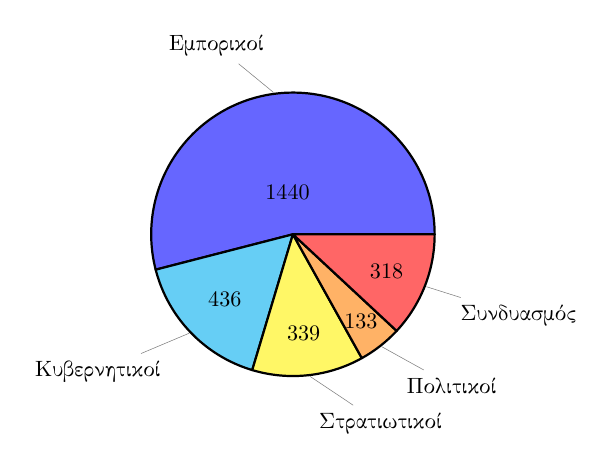
\begin{tikzpicture}[every node/.style={scale=.8}]
	\pie[
	sum=auto,after number=,radius={1.8},text=pin
	]{1440/Εμπορικοί,
		436/Κυβερνητικοί,
		339/Στρατιωτικοί,
		133/Πολιτικοί,
		318/Συνδυασμός
	}
	
	\end{tikzpicture}
	\caption{Είδη δορυφόρων σε λειτουργία το 2018 \autocite{wood_visualizing_all_2020}}
	\label{fig:satellite_types}
\end{marginfigure}

Η παρούσα εργασία ασχολείται με την Αεροδιαστημική Μηχανική, και πιο συγκεκριμένα την τεχνολογία κατασκευής και χειρισμού δορυφόρων. Ο πρώτος τεχνητός δορυφόρος "Sputnik 1" εκτοξεύτηκε το έτος 1957, και μέχρι το 2021 έχουν εκτοξευτεί περίπου \SI{8900}{} δορυφόροι, από τους οποίους περίπου \SI{4000}{} είναι λειτουργικοί και σε τροχιά \autocite{unionofconcernedscientists_satellite_database_2021,kelso_norad_twoline,wood_visualizing_all_2020}.

Οι εκτοξευμένοι δορυφόροι επιτελούν ένα σύνολο από διαφορετικές λειτουργίες, που μπορεί να περιλαμβάνουν τηλεπικοινωνίες, παρατήρηση γης, σήματα πλοήγησης (\acs{GNSS}), \g{επιστημονική έρευνα, ανάπτυξη τεχνολογίας ή άλλους σκοπούς, χωρίς να συμπεριλαμβάνονται σε αυτό το κομμάτι επανδρωμένες αποστολές, αποστολές εκτός της τροχιάς της γης, ή διαστημικοί σταθμοί. Τα δεδομένα που παράγει η διαστημική τεχνολογία, με επιδράσεις στις μεταφορές, στην πρόγνωση καιρού και στην τεχνολογία, έχουν εδώ και καιρό γίνει αναπόσπαστο κομμάτι του σύγχρονου πολιτισμού.}

\begin{figure}
	\centering
	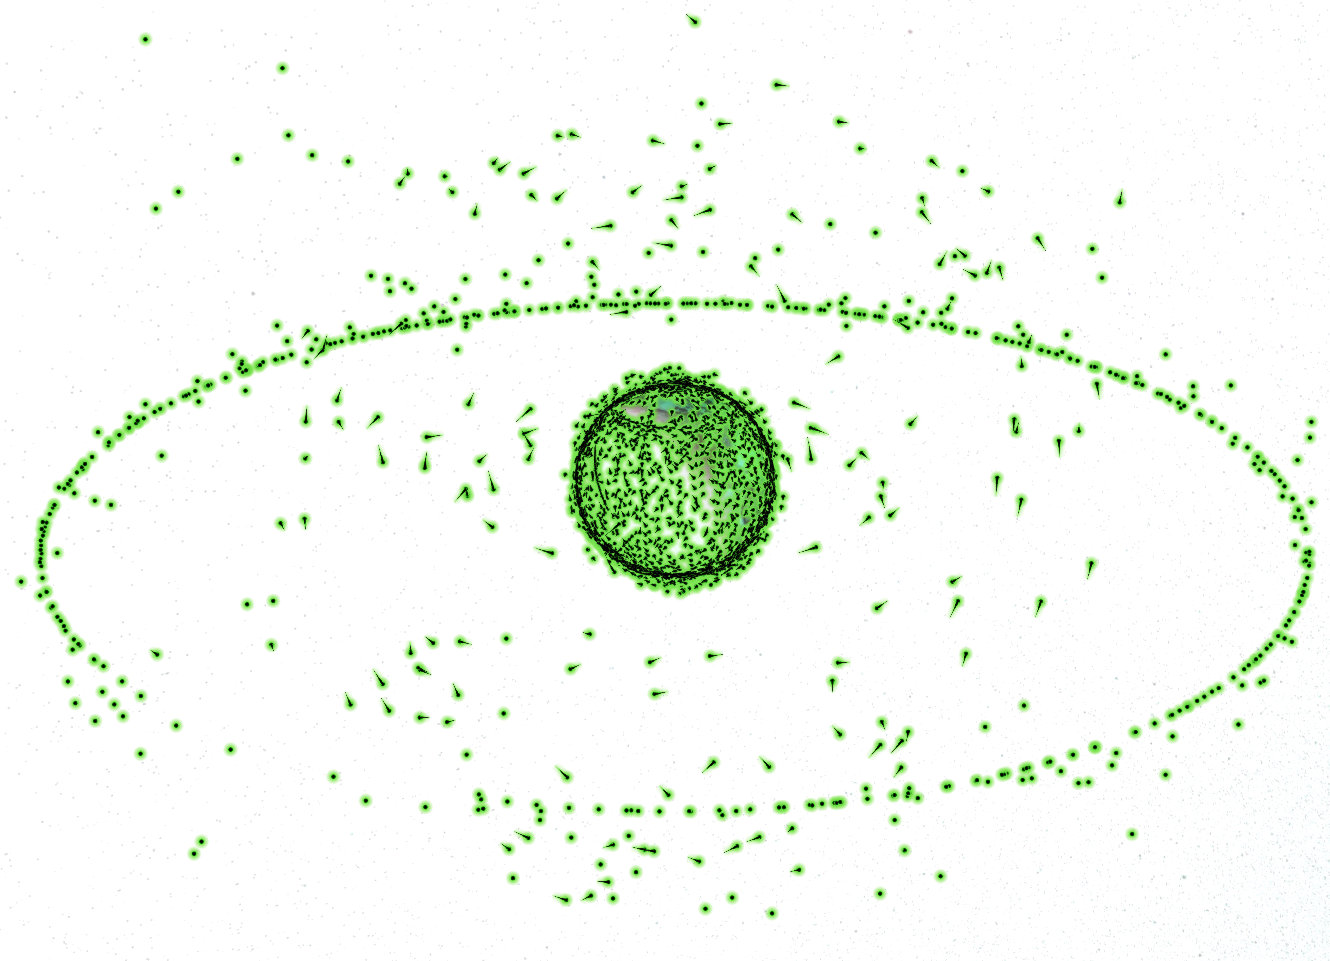
\includegraphics[width=.9\textwidth]{satellites}
	\caption[Ενεργοί δορυφόροι σε τροχιά γύρω από τη γη το 2021]{Ενεργοί τεχνητοί δορυφόροι σε τροχιά γύρω από τη γη το 2021. Κοντά στον πλανήτη βρίσκονται οι δορυφόροι Χαμηλής Γήινης Τροχιάς. Σε σταθερό υψόμετρο \SI{35786}{\kilo\meter} βρίσκονται οι δορυφόροι Γεωστατικής τροχιάς, και ανάμεσά τους κινούνται οι δορυφόροι Μέσης Γήινης Τροχιάς \autocite{agi:analyticalgraphics_satellite_viewer}}
	\label{fig:all_satellites}
	\setfloatalignment{t}
\end{figure}

Μετά την εκτόξευσή τους, οι δορυφόροι τυπικά παραμένουν στο διάστημα μέχρι την ολοκλήρωση της αποστολής τους μετά από κάποια χρόνια, οπότε και μπορούν να επιστρέψουν στη γη και να καούν στην ατμόσφαιρα, είτε να παραμείνουν στο διάστημα ως διαστημικά σκουπίδια.

\begin{marginfigure}
	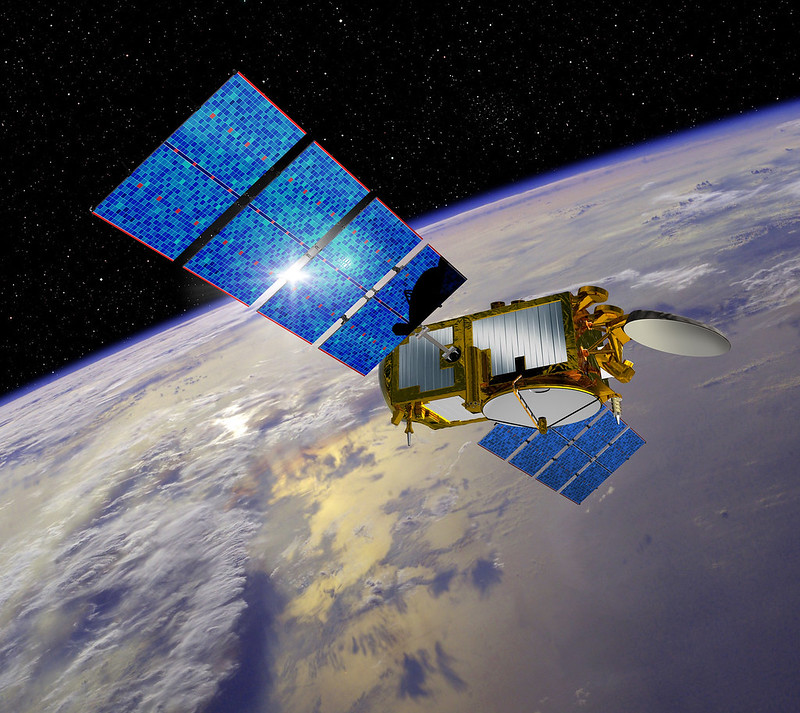
\includegraphics{cool_satellite}
	\caption[Γραφική αναπαράσταση του δορυφόρου Jason-3]{Γραφική αναπαράσταση του δορυφόρου \href{https://www.flickr.com/photos/noaasatellites/16979948568}{Jason-3}. %Στην εικόνα διακρίνονται τα ηλιακά πάνελς, οι δύο κατευθυντικές κεραίες και η θερμική μόνωση του δορυφόρου.
	}
\end{marginfigure}

\g{Η ανάπτυξη διαστημικής τεχνολογίας παρουσιάζει έναν σημαντικό βαθμό δυσκολίας, ο οποίος προέρχεται από τις ιδιαίτερα αυξημένες απαιτήσεις αξιοπιστίας στις δυσμενείς συνθήκες του διαστήματος. Πιο συγκεκριμένα, η μεγάλη απόσταση, οι ακραίες θερμοκρασίες, τα μηχανικά φορτία της εκτόξευσης, οι ακτινοβολίες υψηλών ενεργειών, το κενό αέρα,  και η αδυναμία αποκατάστασης βλαβών, έχουν εγείρει ένα ευρεί φάσμα προκλήσεων μπροστά στην εξερεύνηση του διαστήματος. Έτσι, πέρα από την τυπική ανάπτυξη τεχνολογίας, τα πρότζεκτ αεροδιαστημικής συνδέονται αναπόσπαστα με ένα σύνολο κλάδων της μηχανικής, όπως το} systems engineering (μηχανική συστημάτων), product assurance (διασφάλιση ποιότητας), reliability engineering (αξιοπιστία συστημάτων) και ζητήματα assembly, integration \& verification (κατασκευής, συναρμολόγησης και επαλήθευσης) \autocite{smad}. Η παρούσα εργασία εστιάζει στο κομμάτι \acf{FDIR}, δηλαδή στη δυνατότητα των διαστημικών συστημάτων να εντοπίζουν και να ανακάμπτουν αυτόματα από σφάλματα και λειτουργικές αστοχίες.

Παρά τις προαναφερθείσες δυσκολίες, η επιστήμη έχει προχωρήσει αρκετά ώστε το διάστημα να αποτελεί έναν εμπορικό στόχο. Στα πλαίσια της φιλοσοφίας "NewSpace", όλο και περισσότεροι κερδοσκοπικοί ή μη φορείς εκμεταλλεύονται τις δυνατότητες που προσφέρονται έξω από τη γη \autocite{denis_new_space_2020}. Start-ups, αστερισμοί δορυφόρων, εκπαιδευτικές αποστολές και εμπορικές υπηρεσίες είναι έννοιες που ήδη έγιναν συνηθισμένες τη δεκαετία του 2010, με περισσότερες χώρες ανά τον κόσμο να αρχίζουν όχι μόνον να έχουν πρόσβαση στο διάστημα, αλλά και να αποκτούν δυνατότητα εκτόξευσης.

\begin{marginfigure}
	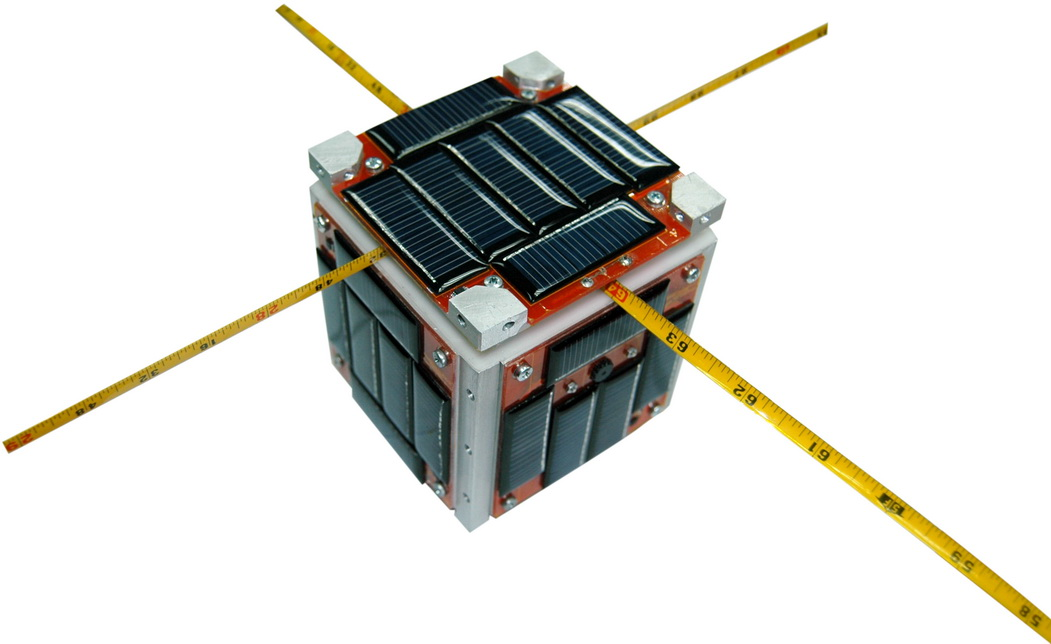
\includegraphics{f1_cubesat_fm}
	\caption{Το "F-1" CubeSat του FPT Πανεπιστημίου στο Βιετνάμ, μεγέθους 1U}
	\label{fig:cubesat}
\end{marginfigure}

Στα πλαίσια του παραπάνω μελετάται η τεχνολογία των όλο και πιο δημοφιλών \textbf{νανοδορυφόρων} \autocite{sweeting_modern_small_2018a}. Τα \textbf{CubeSats}, η πιο δημοφιλής κατηγορία νανοδορυφόρου που είναι και το αντικείμενο αυτής της εργασίας, δημιουργήθηκαν σαν ιδέα το 1999. Το χαμηλό τους κόστος και μέγεθος, καθώς και η μικρή σχετικά πολυπλοκότητα, έχουν επιτρέψει πανεπιστήμια και οργανισμούς παγκοσμίως να εκτοξεύσουν πάνω από \SI{1530}{} CubeSats \autocite{swartwout_cubesat_database_2021}.

Τα CubeSats κατασκευάζονται από δομικές μονάδες διαστάσεων \SI[product-units = single]{10 x 10 x 10}{\centi\metre} που ονομάζονται \textbf{Units}. Τυπικά μεγέθη δορυφόρων προκύπτουν "στοιβάζοντας" αυτά τα units, \g{με αποτέλεσμα δορυφόρους} 1U, 1.5U, 2U, 3U, 6U και 12U. Το κάθε Unit να μπορεί να ζυγίσει μέρχι \SI{2}{\kilogram}. Εσωτερικά, τα CubeSat αποτελούνται από εμπορικά ηλεκτρονικά εξαρτήματα χαμηλού κόστους, τα λεγόμενα \acf{COTS}. Τα CubeSats εκτοξεύονται συνήθως σε Χαμηλή Γήινη Τροχιά (\acs{LEO}) \autocite{anthopoulos_orbital_analysis_2020,riebeek_catalog_earth_2009}, \g{τοποθετούμενα ως δευτερεύοντα φορτία σε εκτοξεύσεις μεγαλύτερων δορυφόρων }("piggyback launch")\g{, και παραμένουν ενεργά για χρονικά διαστήματα περίπου 1 ως 3 χρόνια.}

\section{Σκοπός και Συνεισφορά της Εργασίας}

\begin{marginfigure}
	\centering
	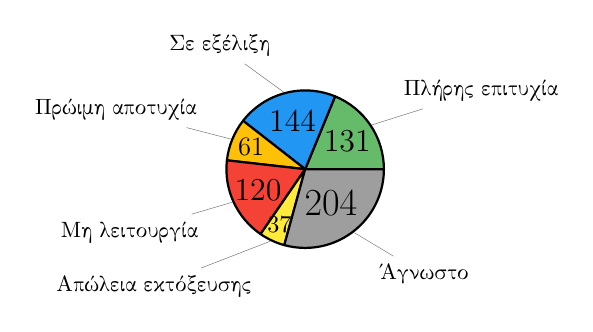
\begin{tikzpicture}[every node/.style={scale=0.8}]
	\pie[
	sum=auto,after number=,radius={1},text=pin,rotate=0,scale font,color={MaterialGreen400, MaterialBlue, MaterialAmber, MaterialRed, MaterialYellow, MaterialGrey}
	]{131/Πλήρης επιτυχία,
		144/Σε εξέλιξη,
		61/Πρώιμη αποτυχία,
		120/Μη λειτουργία,
		37/{Απώλεια εκτόξευσης},
		204/Άγνωστο
	}
	
	\end{tikzpicture}
	\caption{Κατάσταση αποστολών CubeSat από το 2000 \autocite{swartwout_cubesat_mission_2019}}
	\label{fig:cubesat_status}
\end{marginfigure}

\begin{marginfigure}
	\centering
	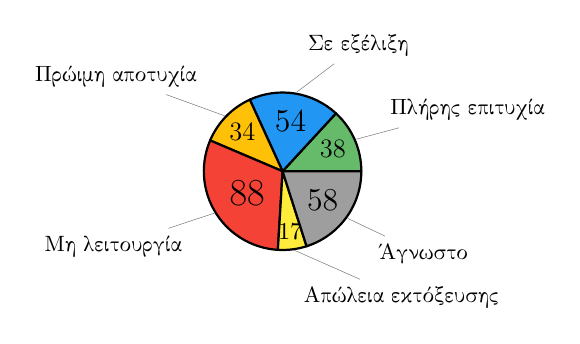
\begin{tikzpicture}[every node/.style={scale=0.8}]
	\pie[
	sum=auto,after number=,radius={1},text=pin,rotate=0,scale font,color={MaterialGreen400, MaterialBlue, MaterialAmber, MaterialRed, MaterialYellow, MaterialGrey}
	]{38/Πλήρης επιτυχία,
		54/Σε εξέλιξη,
		34/Πρώιμη αποτυχία,
		88/Μη λειτουργία,
		17/{Απώλεια εκτόξευσης},
		58/Άγνωστο
	}
	
	\end{tikzpicture}
	\caption[Κατάσταση αποστολών CubeSat από ανεξάρτητους κατασκευαστές]{Κατάσταση αποστολών CubeSat από "hobbyists" (πανεπιστήμια και άλλα ερευνητικά/εκπαιδευτικά πρότζεκτ) \autocite{swartwout_cubesat_database_2021}}
	\label{fig:cubesat_status_hobbyist}
\end{marginfigure}

Η παρούσα εργασία αφορά τη βελτίωση της \textbf{αξιοπιστίας} των νανοδορυφόρων και συστημάτων CubeSat. Αν και η πλειοψηφία των κλασικών δορυφόρων που έχουν εκτοξευτεί είχαν, έστω μερικώς, επιτυχημένες αποστολές \autocite{kattakuri_failures_spacecraft_2019,jacklin_smallsatellite_mission_2019}, το 39.6\% των εκτοξευμένων CubeSats έχουν αποτύχει να ολοκληρώσουν την αποστολή τους, ή δεν έχουν λειτουργήσει σε τροχιά. Το ποσοστό αποτυχίας αυξάνεται στο 57.0\% αν εστιάσουμε σε φορείς (όπως Πανεπιστήμια) που εκτοξεύουν τα πρώτα τους CubeSat, και δεν διαθέτουν το διαστημικό υπόβαθρο των μεγάλων κατασκευαστών και των εμπορικών δορυφόρων.

Οι λόγοι της υψηλής αποτυχίας των CubeSat σχετίζονται κυρίως με το συμπιεσμένο πρόγραμμα κατασκευής, το οποίο οδηγεί σε σφάλματα και προβλήματα που δεν εντοπίζονται κατά τη διάρκεια του σχεδιασμού. Πηγές βλαβών όπως περιβαλλοντική φθορά (θερμικοί κύκλοι, ακτινοβολία), έλλειψη περιθωρίων ασφαλείας στην ισχύ και τις τηλεπικοινωνίες, και προβλήματα λογισμικού, συνδυάζονται με τη γενικότερη έλλειψη εμπειρίας και αυστηρών διαδικασιών των νέων κατασκευαστών, για να μειώσουν το βαθμό αξιοπιστίας των νανοδορυφόρων \autocite{swartwout_cubesat_mission_2019,langer_reliability_estimation_2017}.

Η προσέγγιση που ακολουθείται για την αύξηση της αξιοπιστίας των CubeSat περιλαμβάνει:
\begin{compactitem}
	\item Μείωση του αριθμού πιθανών βλαβών από την φάση του σχεδιασμού, με συμπερίληψη ζητημάτων αξιοπιστίας στις πρώιμες φάσεις του πρότζεκτ
	\item Δομημένα εργαλεία εκτίμησης και βελτίωσης της αξιοπιστίας, όπως \textbf{\acf{FMEA}} και \textbf{\acf{FDIR}} \autocite{faure_lean_satellites_2017,menchinelli_reliability_engineering_2018}
	\item \g{Προσαρμογή και υιοθέτηση ανοιχτών προτύπων διαστημικής τεχνολογίας για το σχεδιασμό, την κατασκευή και την επαλήθευση} \autocite{scholz_handbook_free_2021}
\end{compactitem}

\begin{figure}
	\centering
	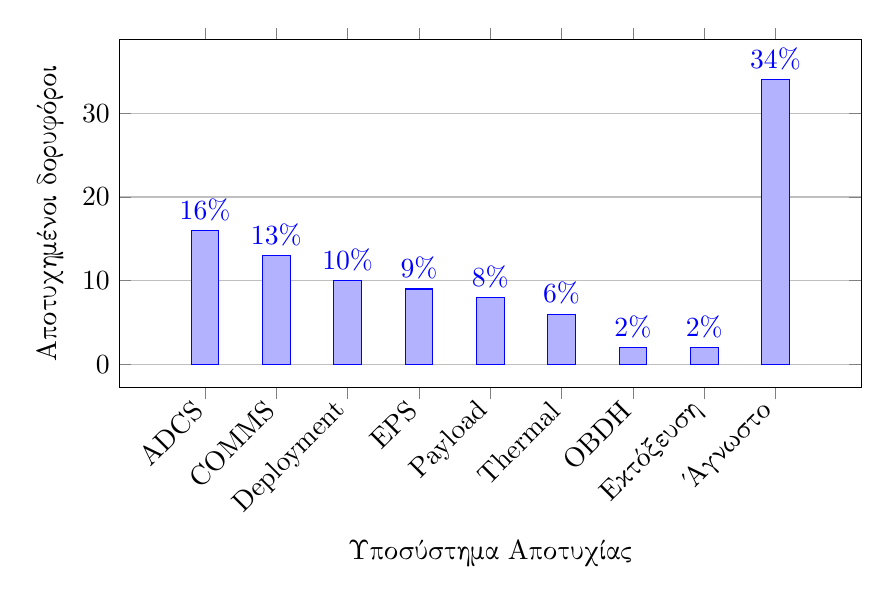
\begin{tikzpicture}
	\begin{axis}  
	[  
	ybar,  
	enlargelimits=0.15,  
	ylabel={Αποτυχημένοι δορυφόροι}, % the ylabel must precede a # symbol.  
	xlabel={Υποσύστημα Αποτυχίας},  
	symbolic x coords={ADCS, COMMS, Deployment, EPS, Payload, Thermal, OBDH, Launch, Unknown}, % these are the specification of coordinates on the x-axis.  
	xticklabels={ADCS, COMMS, Deployment, EPS, Payload, Thermal, OBDH, Εκτόξευση, Άγνωστο},
	xtick=data,  
	nodes near coords, % this command is used to mention the y-axis points on the top of the particular bar.  
	nodes near coords align={vertical},  
	ymajorgrids={true},
	width=11cm,
	height=6cm,
	x tick label style={rotate=45,anchor=east},
	nodes near coords={\pgfmathprintnumber\pgfplotspointmeta\%} 
	]  
	\addplot coordinates {(ADCS, 16) (COMMS, 13) (Deployment, 10) (EPS, 9) (Payload, 8) (Thermal, 6) (OBDH, 2) (Launch, 2) (Unknown, 34) };  
	
	\end{axis}  
	\end{tikzpicture}  
	\caption[Κύριοι λόγοι αποτυχίας αποστολών CubeSat]{Κύριοι λόγοι αποτυχίας αποστολών CubeSat (\(n=50\)) \autocite{bouwmeester_survey_implementation_2017}}
	\label{fig:whyfail}
\end{figure}


Η παρούσα εργασία σκοπεύει να εμπλουτίσει την εργαλειοθήκη των κατασκευαστών CubeSat αναλύοντας μία δομημένη προσέγγιση \ac{FDIR} που βασίζεται στα \textbf{ευρωπαϊκά πρότυπα \acs{ECSS}}, και στην εργασία της πρωτοβουλίας \textbf{\acs{SAVOIR}}\footurl{https://savoir.estec.esa.int/} της ευρωπαϊκής διαστημικής βιομηχανίας. Στις επόμενες σελίδες, θα αναλυθεί πως οι ιδέες αυτές μπορούν να προσαρμοστούν σε μία αποστολή CubeSat μικρού βεληνεκούς ώστε:
\begin{itemize}
	\item Να χρησιμοποιηθεί ένας δομημένος τρόπος για να ερευνηθούν οι πιθανές αποτυχίες ενός δορυφόρου, και τρόποι αντιμετώπισής τους
	\item Να προετοιμαστεί λογισμικό που θα μπορεί να ανταποκριθεί και να διαχειριστεί με ασφάλεια το σύνολο των κρίσιμων αποτυχιών σε τροχιά
	\item Να αναπτυχθεί μία \textbf{παραμετροποιήσιμη} αρχιτεκτονική, που θα επιτρέπει τους χειριστές να μεταβάλλουν εύκολα τη συμπεριφορά του συστήματος \acs{FDIR} και να το προσαρμόσουν σε διαφορετικά δεδομένα
\end{itemize}

Το προτεινόμενο σύστημα \acs{FDIR} στοχεύει στην αύξηση της σιγουριάς κατά την κατασκευή, αλλά και στη γρήγορη ενσωμάτωση νέων δεδομένων που προκύπτουν κατά τις δοκιμές και την εκτόξευση.

Πέρα από τη θεωρητική ανάλυση, περίληψη και σχολιασμό των προτύπων, η εργασία εστιάζει στην εφαρμογή της προαναφερθείσας δομής \acs{FDIR} στο νανοδορυφόρο \emph{AcubeSAT}, και περιλαμβάνει μία πειραματική υλοποίηση της σουίτας \acs{FDIR} σε υλικό \& λογισμικό.

% maybe some other inspiring stuff here? idk

\section{Διάρθωση και Δομή}

Η εργασία ξεκινάει με την περίληψη της αποστολής AcubeSAT, που αποτελεί την κύρια αφορμή και πλαίσιο συγγραφής της (\Cref{cap:acubesat}). Συνεχίζει με μία ανάλυση των κύριων προτύπων και της φιλοσοφίας \acs{FDIR}, με εστίαση στα κομμάτια που αφορούν τους κατασκευαστές CubeSat και τις ερευνητικές ή εκπαιδευτικές αποστολές (\Cref{cap:savoir}). Το επόμενο κομμάτι εξετάζει την εφαρμογή των προηγούμενων προτύπων στο σχεδιασμό του AcubeSAT, και σε μερικές σχεδιαστικές αποφάσεις και λεπτομέρειες υλοποίησης του \acs{FDIR} στο νανοδορυφόρο (\Cref{cap:acufdir}).

Το τελευταίο κεφάλαιο περιλαμβάνει την πρακτική επίδειξη του προτεινόμενου \acs{FDIR} \g{σε ένα απλό δοκιμαστικό σύστημα δύο αισθητήρων} (\Cref{cap:practical}). Το σύστημα αναπτύσσεται έτσι ώστε να μπορεί να εντοπίσει και να ανακάμψει από όλες τις προβλεπόμενες πιθανές αποτυχίες, χρησιμοποιώντας τις πλήρεις βιβλιοθήκες που καλύπτουν τα πρότυπα \acs{ECSS} και \acs{FDIR}. Μετά από την ανάπτυξη του συστήματος, γίνεται πλήρης δοκιμή της απόκρισής του στις αποτυχίες. Το σύστημα είναι διαμορφωμένο έτσι ώστε να εξομοιώσει το σύστημα του δορυφόρου, συμπεριλαμβανομένου του συστήματος μικροελεγκτή αλλά και του Σταθμού Βάσης.

\chapter{Η αποστολή AcubeSAT}
\label{cap:acubesat}

\begin{marginfigure}
	
\includegraphics{acubesat_patch}
	\caption{Λογότυπο της αποστολής AcubeSAT}
\end{marginfigure}

\begin{marginfigure}
	\centering
	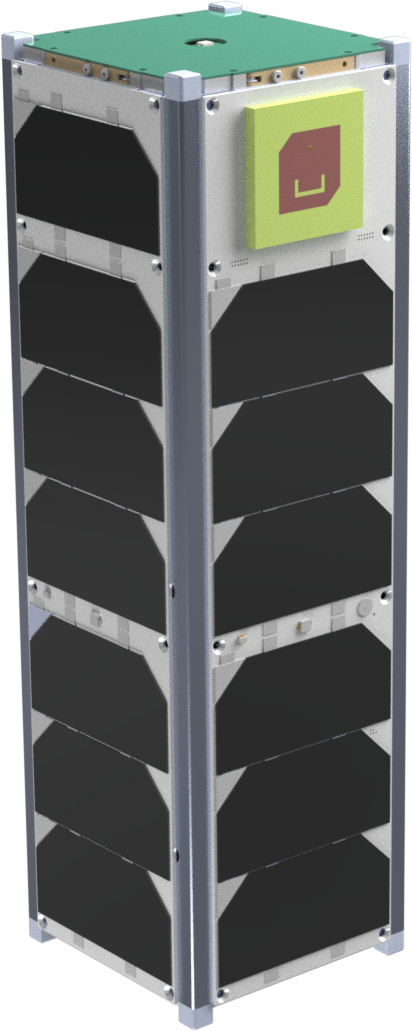
\includegraphics[width=.8\textwidth]{acubesat}
	\caption{Καλλιτεχνική προβολή του νανοδορυφόρου AcubeSAT}
\end{marginfigure}

Το πλαίσιο ανάπτυξης της παρούσας εργασίας είναι το πρότζεκτ του νανοδορυφόρου \textbf{"AcubeSAT"} που βρίσκεται υπό σχεδιασμό από φοιτητές του Αριστοτελείου Πανεπιστημίου Θεσσαλονίκης, και στοχεύει στην εκτέλεση ενός πειράματος βιολογικής φύσεως στο διάστημα.

Το πρότζεκτ ξεκίνησε σε ερευνητική μορφή το 2015, και το 2020 έγινε μέρος του προγράμματος \foothref{https://www.esa.int/Education/CubeSats_-_Fly_Your_Satellite}{Fly Your Satellite! 3} του Ευρωπαϊκού Οργανισμού Διαστήματος (European Space Agency), με ορίζοντα εκτόξευσης το 2023.

Το AcubeSAT έχει μέγεθος 3 κυβικών μονάδων (\textbf{3U}), διαστάσεις \SI[product-units = single]{10 x 10 x 34.05}{\centi\metre} και μάζα \SI{4.26}{\kilogram}. \g{Περιλαμβάνει το \emph{ωφέλιμο φορτίο} του πειράματος, που καλύπτει} 2U, \g{και τα υπόλοιπα υποστηρικτικά υποσυστήματα} (platform) στο υπόλοιπο 1U.

\g{Το πρότζεκτ είναι ανοιχτού κώδικα, με το λογισμικό και τις κατασκευές που έχει ετοιμάσει οι ομάδα να βρίσκονται στο διαδίκτυο για ελεύθερη χρήση από το κοινό.} \footurl{https://gitlab.com/acubesat/}

\section{Η αποστολή}


Η κύρια αποστολή του AcubeSAT είναι η μελέτη ευκαρυωτικών κυττάρων σε Χαμηλή Γήινη Τροχιά, και πιο συγκεκριμένα η εκτίμηση των αποτελεσμάτων της \emph{ακτινοβολίας} και \emph{μικροβαρύτητας} σε 190 διαφορετικά στελέχη του ζυμομύκητα \emph{Saccharomyces Cerevisiae}. Τα προηγούμενα επιτυγχάνονται με μία πρωτότυπη διάταξη "lab-on-a-chip", η οποία στο κέντρο της έχει ένα τσιπ \textbf{μικρορευστομηχανικής} (\Cref{fig:microfluidic_chip}) \autocite{volpetti_microfluidic_biodisplay_2017} που επιτρέπει την εξέταση της ρύθμισης της μοριακής συμπεριφοράς των κυττάρων σε πρωτοφανή κλίμακα.

Τα αποτελέσματα του πειράματος μεταφέρονται στη Γη σε μορφή φωτογραφιών, όπου συγκρίνονται με ένα όμοιο επίγειο πείραμα.



\begin{figure}[th]
	\centering
	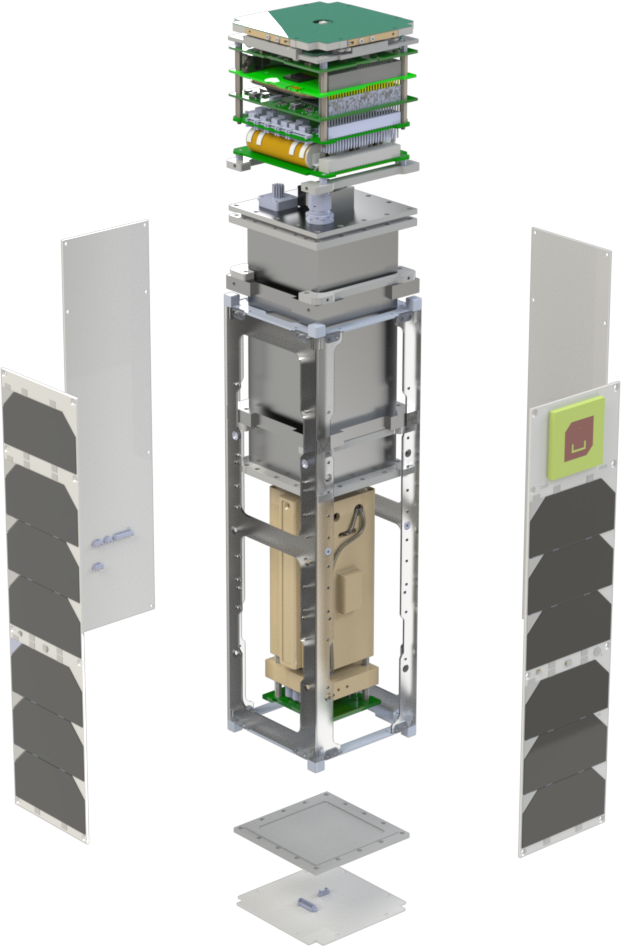
\includegraphics[width=.7\textwidth]{cubesat_exploded}
	\caption{Προβολή του εσωτερικού του AcubeSAT, όπου φαίνονται τα διαφορετικά υποσυστήματα και η πειραματική διάταξη}
\end{figure}

\section{Υποσυστήματα}

Ο νανοδορυφόρος AcubeSAT είναι τεχνικά και οργανωτικά χωρισμένος σε 11 διαφορετικές υποομάδες ή \textbf{υποσυστήματα}, κάθε μία από τις οποίες είναι υπεύθυνη για ένα διαφορετικό τμήμα του δορυφόρου, και αποτελείται από \SIrange{2}{9}{} αφοσιωμένα μέλη.
\begin{marginfigure}
	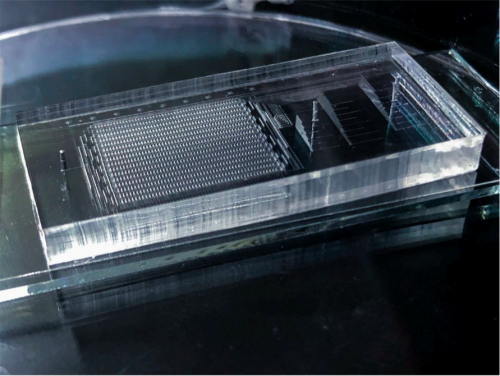
\includegraphics{microfluidic_chip}
	\caption{Δοκιμαστικό μοντέλο του τσιπ μικρορευστομηχανικής}
	\label{fig:microfluidic_chip}
\end{marginfigure}

Στις επόμενες ενότητες παρουσιάζεται μια σύντομη εισαγωγή στη λειτουργία και το σχεδιασμό κάθε υποσυστήματος. Καθώς η διαδικασία σχεδιασμού συστημάτων και \acl{PA} είναι %\ensuregreek{εγ\-γε\-νώς}
\g{εγγενώς}
συνδεδεμένη με τη λειτουργία όλων των υποσυστημάτων, \g{αναφέρονται} επίσης οι λεπτομέρειες που αφορούν το \acs{FDIR}. Για πιο λεπτομερείς πληροφορίες, ο αναγνώστης ενθαρρύνεται να ανατρέξει στην \foothref{https://acubesat.spacedot.gr/subsystems/}{ιστοσελίδα του AcubeSAT}, ή στα δημοσίως διαθέσιμα \foothref{https://gitlab.com/acubesat/documentation/cdr-public}{έγγραφα του \ac{CDR}}.

\subsection{Υποσύστημα Προσδιορισμού και Ελέγχου Προσανατολισμού (\acs{ADCS})}
\label{sec:adcs}

Η υποομάδα του \ac{ADCS} είναι υπεύθυνη για τον έλεγχο του \textbf{προσανατολισμού} του δορυφόρου σε τροχιά. Αυτό επιτυγχάνεται με τη χρήση μιας σειράς ενεργοποιητών, που προέρχονται έτοιμοι από την αγορά (\ac{COTS}): μία πλακέτα 3 αξόνων και έναν τροχός αντίδρασης 1 άξονα, σε συνδυασμό με αισθητήρες για τον προσδιορισμό της περιστροφής του δορυφόρου (1 γυροσκόπιο και 2 μαγνητόμετρα) και αλγορίθμους φιλτραρίσματος \& ελέγχου \autocite{DDJF_AOCS,velentzas_design_attitude_2021}.

Το \ac{ADCS} μπορεί να λειτουργήσει με τα εξής διαφορετικά ``προφίλ στόχευσης'' (pointing profiles) για να καλύψει διαφορετικές λειτουργικές ανάγκες:
\begin{enumerate}
	\item \textbf{Λειτουργία Σταθεροποίησης} (Detumbling), όπου ο δορυφόρος προσπαθεί να φτάσει τη γωνιακή του ταχύτητα κοντά στο 0, για να εξασφαλίσει μια αξιόπιστη ραδιοζεύξη, να αποτρέψει την αποκόλληση εξαρτημάτων και να επιτρέψει αργότερα την ευκολότερη ανάκτηση του επιθυμητού προσανατολισμού.
	
	Η λειτουργία Σταθεροποίησης υλοποιείται με τον απλούστερο δυνατό τρόπο, χρησιμοποιώντας μόνο το ένα από τα 2 μαγνητόμετρα και έναν απλό αλγόριθμο ελέγχου. Ενεργοποιείται όταν δεν υπάρχει ανάγκη εφαρμογής κάποιου άλλου ή όταν η γωνιακή ταχύτητα του νανοδορυφόρου είναι επικίνδυνα υψηλή.
	
	\item \textbf{Στόχευση στο Ναδίρ} (Nadir Pointing), όπου ο δορυφόρος \g{στρέ\-φει} την πλευρά \(+X\) ώστε να κοιτάζει προς τη Γη. Αυτό το προφίλ χρησιμοποιείται σε περάσματα πάνω από τον Σταθμό Βάσης, όπου η κατευθυντική κεραία χρειάζεται άμεση ορατότητα.
	
	\item \textbf{Στόχευση στον Ήλιο} (Sun Pointing), όπου ο δορυφόρος \g{στρέφεται} προς τον ήλιο, προ\-κει\-μέ\-νου να μεγιστοποιηθεί η είσοδος των ηλιακών πάνελ. Αυτό το προφίλ χρησιμοποιείται ανάμεσα στα περάσματα από το Σταθμό Βάσης, προκειμένου να εξασφαλιστεί θετικός προϋπολογισμός ισχύος.
\end{enumerate}

\begin{margintable}
	\centering
	\caption[Μέγιστες τιμές σφαλμάτων ADCS μετά τη σταθεροποίηση]{Μέγιστες τιμές σφαλμάτων \ac{ADCS} μετά τη σταθεροποίηση}
	\label{tab:adcsape}
	\begin{tabular}{@{}ll@{}}
		\toprule
		Σφάλμα                      & Τιμή                    \\ \midrule
		Απόλυτη Ακρίβεια Στόχευσης & \( < \SI{30}{\degree} \) \\
		Απόλυτη Ακρίβεια Γνώσης    & \( < \SI{1}{\degree} \) 
	\end{tabular}
\end{margintable}

%Οι επιδόσεις του \ac{ADCS} μπορούν να αξιολογηθούν με μετρικές όπως αυτές που παρουσιάζονται στον \Cref{tab:adcsape}.

\subsection{Υποσύστημα Τηλεπικοινωνιών (\acs{COMMS})}

Το υποσύστημα communications (τηλεπικοινωνιών) είναι υπεύθυνο για τη μετάδοση δεδομένων μεταξύ της Γης και του δορυφόρου σε τροχιά. Τα μεταδιδόμενα δεδομένα χωρίζονται σε 3 διαφορετικές κατηγορίες\autocite{DDJF_TTC}:
\begin{itemize}
	\item \textbf{\acf{TC}}: Εντολές από τη Γη προς το δορυφόρο. Μπορούν να χρησιμοποιηθούν για να ζητήσουν πληροφορίες ή για να εκτελέσουν συγκεκριμένες ενέργειες στο CubeSat.
	\item \textbf{\acf{TM}}: Πληροφορίες που αποστέλλονται από τον δορυφόρο προς τη Γη, που συνήθως περιλαμβάνουν ζωτικές πληροφορίες, όπως τιμές αισθητήρων, κατάσταση συστήματος, τρέχουσα ώρα και συμβάντα.
	\item \textbf{Επιστημονικά δεδομένα}: Τα επιστημονικά δεδομένα που παράγονται από το ωφέλιμο φορτίο (payload). Αυτά είναι τα δεδομένα με τον μεγαλύτερο όγκο και αντιπροσωπεύουν τα κύρια  αποτελέσματα της αποστολής.
\end{itemize}

Είναι σημαντικό να αναφερθεί ότι η τροχιά του δορυφόρου επιτρέπει μόνο μια πολύ μικρή διάρκεια ορατότητας από τον Σταθμό Βάσης (\acl{GS}) κάθε μέρα, αυξάνοντας τις ανάγκες για αυτονομία και τη σημασία μιας σωστά εφαρμοσμένης μεθόδου \acs{FDIR}.

\begin{marginfigure}
	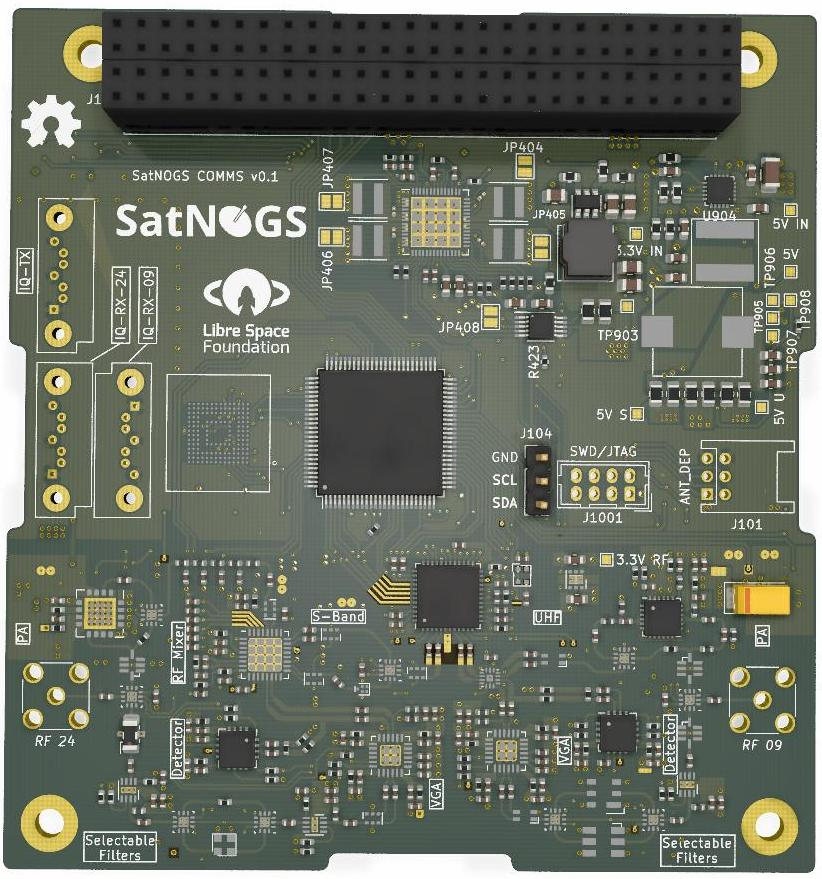
\includegraphics{satnogs-comms}
	\caption{Η πλακέτα SatNOGS COMMS}
\end{marginfigure}

Το κύριο συστατικό του υποσυστήματος \acs{COMMS} είναι η πλακέτα \textbf{SatNOGS COMMS} \autocite{surligas_satnogscomms_2021}, ένας \acs{RF} πομποδέκτης ανοικτού κώδικα που αναπτύσσεται από την \href{https://libre.space/}{LibreSpace Foundation}, βασισμένη στα τηλεπικοινωνιακά πρότυπα \acs{CCSDS}.

Η επικοινωνία πραγματοποιείται με τη χρήση 2 ζωνών συχνοτήτων στην περιοχή \acs{ISM}, \SI{436.5}{\mega\hertz} και \SI{2.425}{\giga\hertz}, μέσω μίας κεραίας διπόλων και μίας κατευθυντικής επιφανειακής κεραίας (patch antenna). Η χρήση των συχνοτήτων \acs{ISM} επιτρέπει την εύκολη ραδιοερασιτεχνική πρόσβαση στο δορυφόρο. Η πρώτη (\acs{UHF}) ζώνη εκπέμπει επίσης ένα περιοδικό σήμα \textbf{beacon} (ραδιοφάρος), που περιέχει κρίσιμες πληροφορίες σχετικά με την κατάσταση του \g{δορυφόρου}.

Το υποσύστημα τηλεπικοινωνιών είναι επίσης υπεύθυνο για την ανάλυση ηλεκτρομαγνητικής συμβατότητας (\acs{EMC}), καθώς και για το σχεδιασμό και την κατασκευή του Σταθμού Βάσης. Ο τελευταίος θα αποτελέσει μέρος του \textbf{SatNOGS}\autocite{white_overview_satellite_2018}, ενός παγκόσμιου δικτύου δορυφορικών επίγειων σταθμών που βασίζεται σε ανοικτές τεχνολογίες και ανοικτά δεδομένα.

\subsection{Υποσύστημα Ενέργειας (\acs{EPS})}

\begin{margintable}
	\caption{Προϋπολογισμός ισχύος AcubeSAT σε κανονική λειτουργία}
	\label{tab:power_budget}
	\begin{tabularx}{\linewidth}{@{}lX@{}}
		\toprule
		\textbf{Καταναλωτής}            & \textbf{Ισχύς}            \\ \midrule
		\acs{ADCS}          & \SI{1.10}{\watt} \\
		\acs{COMMS}         & \SI{0.85}{\watt} \\
		\acs{EPS}           & \SI{0.99}{\watt} \\
		\acs{OBC}           & \SI{0.12}{\watt} \\
		\acs{SU}            & \SI{0.25}{\watt} \\ \midrule
		Σύνολο               & \SI{3.30}{\watt} \\
		Μέση παραγόμενη ισχύς & \SI{4.24}{\watt} \\ \bottomrule
	\end{tabularx}
\end{margintable}

Το \ac{EPS} είναι το υποσύστημα υπεύθυνο για την παραγωγή, κατανομή και αποθήκευση ηλεκτρικής ενέργειας στον δορυφόρο. Είναι ένα κρίσιμο κομμάτι του CubeSat, λόγω της άμεσης εξάρτησης και των σχετικά αυξημένων ενεργειακών αναγκών πολλών υποσυστημάτων του, και θεωρείται πως είναι ο πιο πιθανός λόγος αποτυχίας των CubeSat σε τροχιά \autocite{langer_reliability_cubesats_2016}.

Το AcubeSAT έχει επιλέξει έναν συνδυασμό από \ac{COTS} προϊόντα για το \ac{EPS}: \autocite{DDJF_SYS}
\begin{itemize}
	\item Τα \textbf{ηλιακά πάνελ} (solar panels) αγοράζονται από την EnduroSat. 4 πάνελ διάστασης 3U καλύπτουν τις \(X\) και \(Y\) πλευρές, και ένα πάνελ 1U καλύπτει την \(-Z\) πλευρά.
	\item Η μονάδα \textbf{ελέγχου και διανομής ισχύος} (\acs{PCDU}) αγοράζεται από την NanoAvionics και προσφέρει 10 προστατευμένα κανάλια με 4 διαφορετικές τιμές τάσης, καθώς και 4 μετατροπείς \acs{MPPT}.
	\item Οι \textbf{μπαταρίες}, επίσης αγορασμένες από τη NanoAvionics, \g{αποτελούνται από 4 στοιχεία ιόντων λιθίου μορφής 18650.}
\end{itemize}


\FloatBarrier
\begin{comment}
A dynamic approach is taken with regards to power budget calculation:
\begin{compactenum}
	\item The in-orbit power generation is calculated for the duration of the mission using the \textbf{STK} software, taking into account satellite orientation, pointing profiles and eclipse, with a \SI{1}{\minute} resolution.
	\item The power consumption of the system is calculated on average for each different operational mode.
	\item \acs{MPPT} efficiencies and battery charge level are calculated for each timepoint, assuming worst-case thermal and electrical conditions
	\item A system-wide 10\% margin is applied to the results
\end{compactenum}


We have created a Python library consolidating the above steps\footurl{https://gitlab.com/acubesat/eps/power-budget} and producing the necessary outputs to prove the adequacy of the design.
\end{comment}


\begin{figure*}[h]
%	\begin{subfigure}[b]{.45\textwidth}
	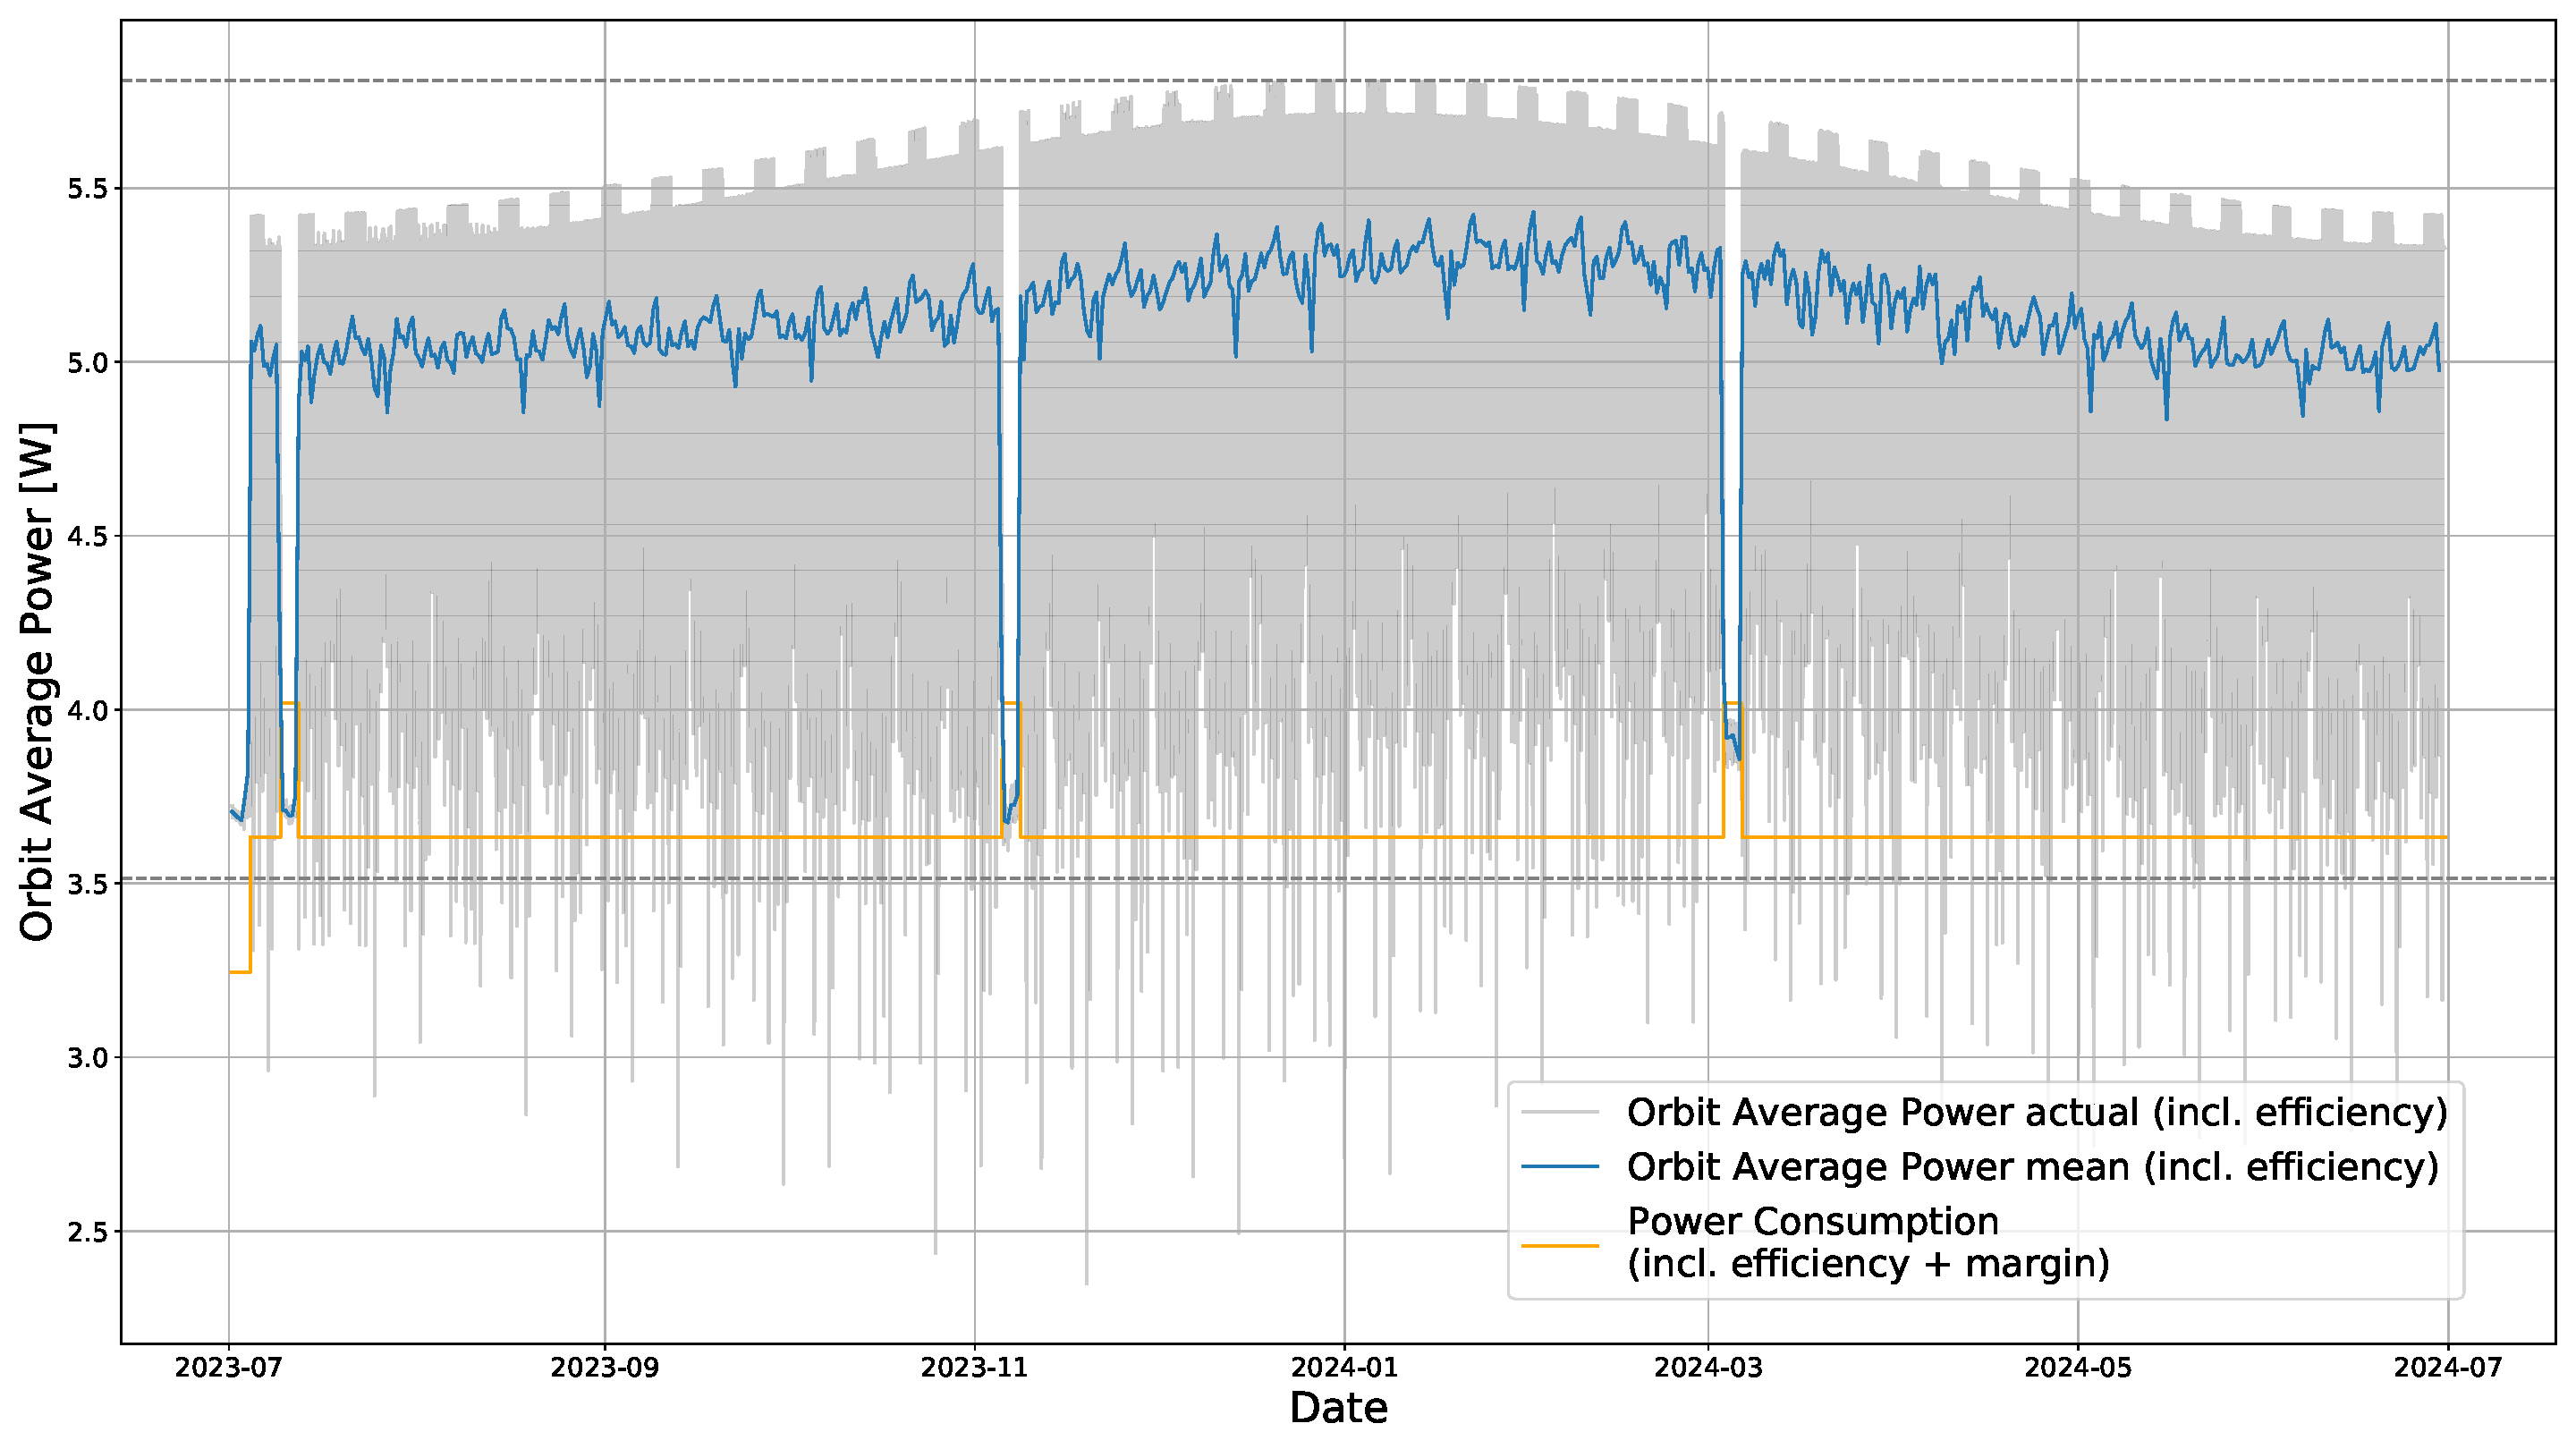
\includegraphics[height=4cm]{Sun Pointing 11:00.total.pdf}
%	\end{subfigure}
	\hfill
%	\begin{subfigure}[b]{.45\textwidth}
	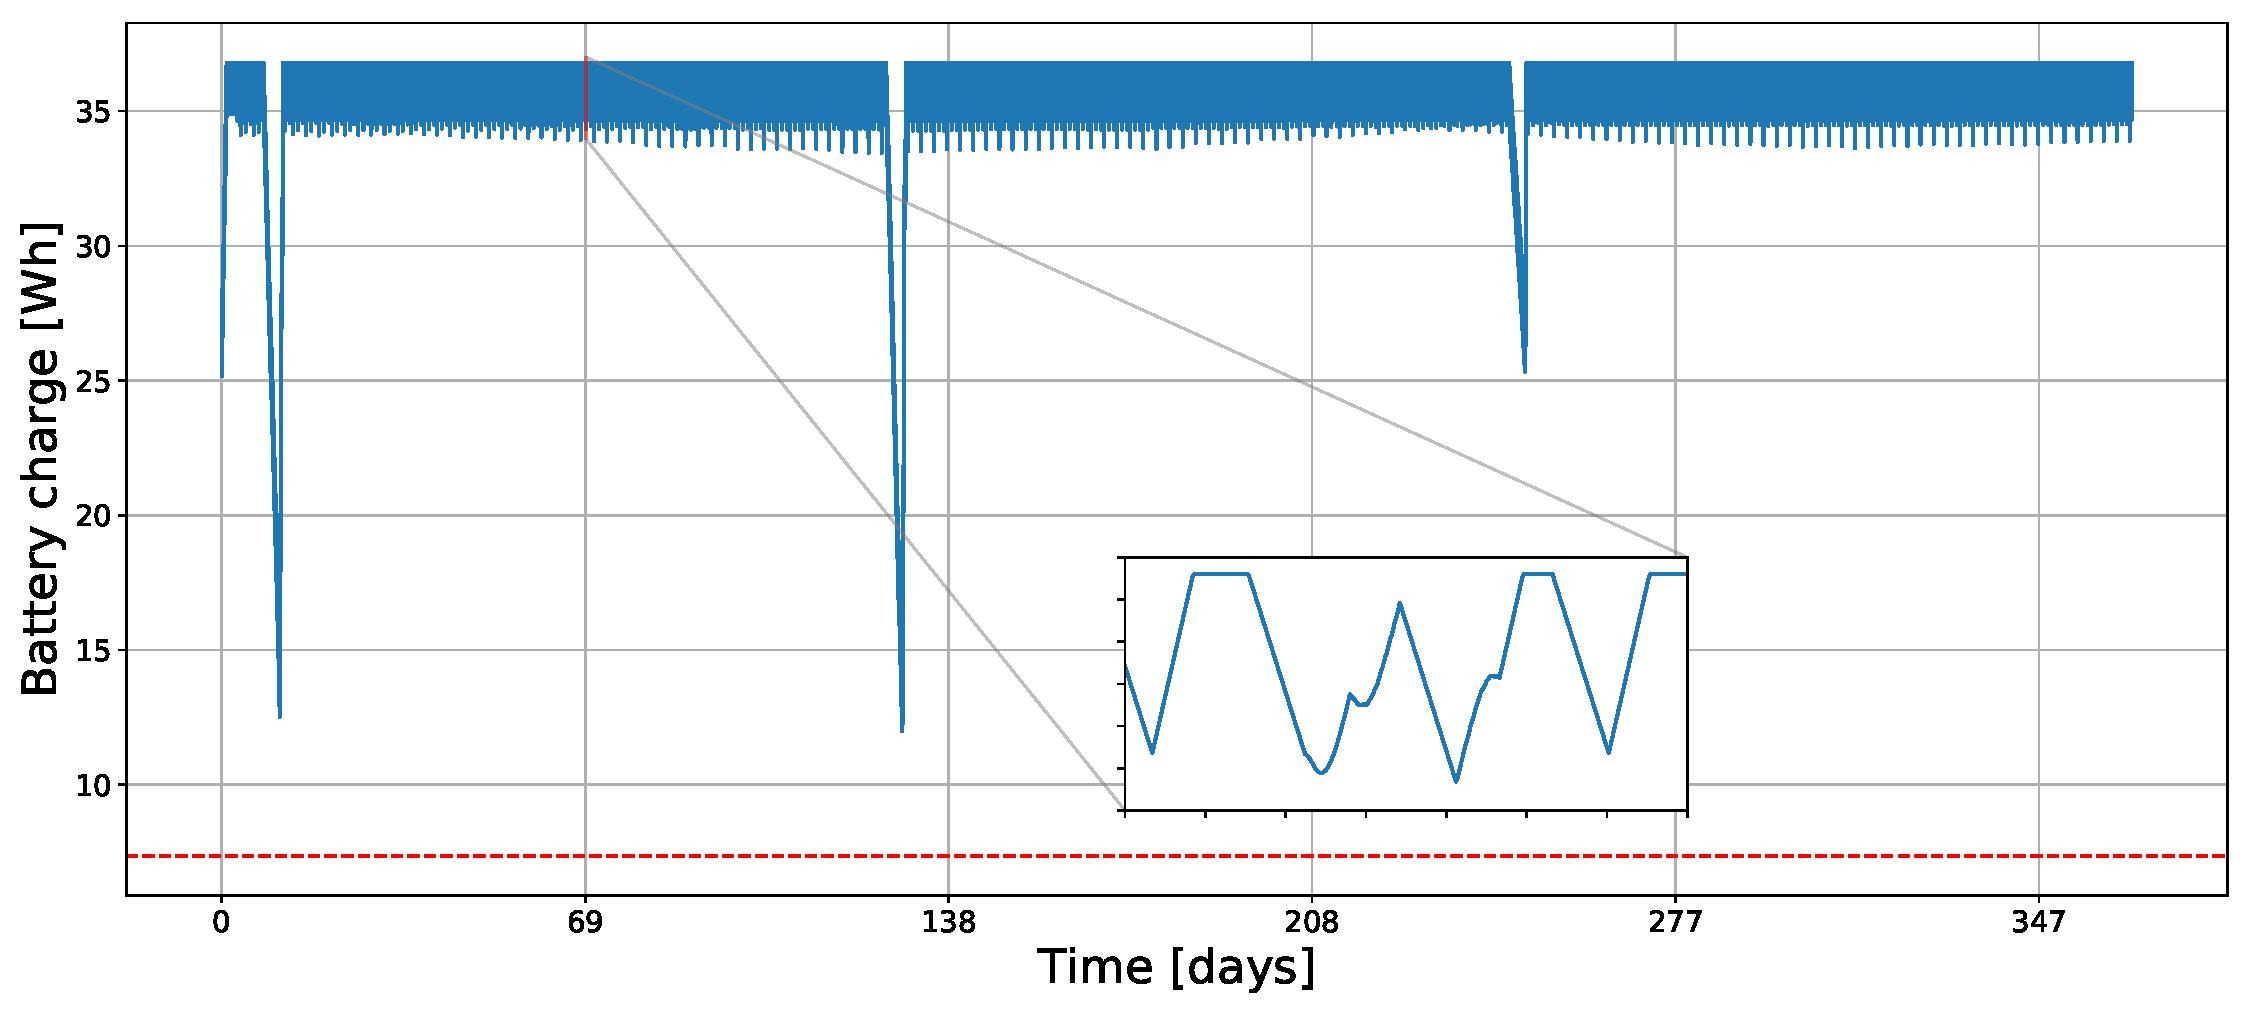
\includegraphics[height=4cm]{Sun Pointing 11:00.discharge.pdf}
%	\end{subfigure}
%	\includegraphics[width=.45\textwidth]{/home/kongr45gpen/Pictures/jeka8ara kapoglis.png}

	\caption[Δυναμική ανάλυση προϋπολογισμού ισχύος]{Δυναμική ανάλυση προϋπολογισμού ισχύος. Αριστερά: Κατανάλωση \& παραγωγή ισχύος στην τροχιά. Δεξιά: Επίπεδο εκφόρτισης μπαταρίας κατά τη διάρκεια της αποστολής}
\end{figure*}

\subsection{Υποσύστημα Διαχείρισης Δεδομένων (\acs{OBDH})}
\label{sec:obdh}

Το υποσύστημα \ac{OBDH} \g{είναι υπεύθυνο για το σχεδιασμό των διεπαφών δεδομένων του} CubeSat, \g{καθώς και για τον σχεδιασμό της πλακέτας} \textbf{\acf{OBC}}, \g{η οποία είναι επιφορτισμένη με τον έλεγχο των βασικών λειτουργιών του δορυφόρου} \autocite{DDJF_OBDH}.

Η πλακέτα \ac{OBC} περιέχει τα βασικά εργαλεία για την εξασφάλιση της αυτονομίας, και βασίζεται σε έναν ανθεκτικό στην ακτινοβολία μικροελεγκτή \foothref{https://www.microchip.com/wwwproducts/en/SAMV71Q21RT}{Microchip SAMV71Q21RT}, και μια μνήμη \acs{MRAM} που χρησιμοποιείται για την αποθήκευση κρίσιμων δεδομένων. Η πλακέτα φιλοξενεί επίσης τον μικροελεγκτή του υποσυστήματος \ac{ADCS}, ως μέτρο εξοικονόμησης χώρου.

\begin{marginfigure}
	\centering
	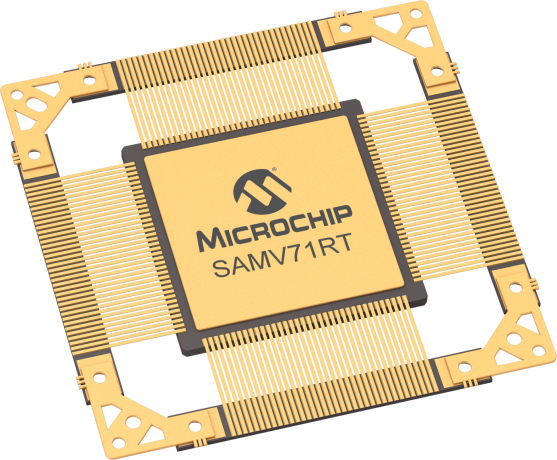
\includegraphics[width=.7\textwidth]{SAMV71Q21RT}
	\caption{Ο μικροελεγκτής \texttt{SAMV71Q21RT}}
	\label{fig:samv71}
\end{marginfigure}

Η διεπαφή δεδομένων μεταξύ των υποσυστημάτων του AcubeSAT χρησιμοποιεί ένα \ac{CAN} bus σε \textbf{ψυχρό πλεονασμό} (cold redundancy), το οποίο επιλέχθηκε λόγω της υψηλής αξιοπιστίας του \autocite{bouwmeester_survey_implementation_2017}. Οι πλακέτες του AcubeSAT ικανοποιούν τις μηχανικές απαιτήσεις του προτύπου PC/104 \autocite{PC104}.

\subsection{Υποσύστημα Λογισμικού (\acs{OBSW})}


Το υποσύστημα \ac{OBSW} είναι υπεύθυνο για το σχεδιασμό και την ανάπτυξη του λογισμικού του νανοδορυφόρου. Η γλώσσα που επιλέχθηκε να χρησιμοποιηθεί στους 4 μικροελεγκτές είναι μια περιορισμένη μορφή της \textbf{C++}, και ο κώδικας ελέγχεται από μια σειρά προτύπων, στατικών αναλυτών και unit tests \autocite{DDJF_OBSW}. Όλο το λογισμικό εκτελείται επάνω στο λειτουργικό σύστημα πραγματικού χρόνου Free\acs{RTOS}.


\subsection{Υποσύστημα Χειρισμού (\acs{OPS})}

Το υποσύστημα Operations \g{είναι υπεύθυνο για το σχεδιασμό των λειτουργιών \& διαδικασιών του σκάφους και για τη διασφάλιση της λειτουργικότητας, της δυνατότητας ελέγχου και της παρατηρησιμότητας του δορυφόρου πριν και κατά τη διάρκεια της τροχιάς του.}

Κατά τη διάρκεια της αποστολής, το AcubeSAT μπορεί να βρίσκεται σε μία από τις ακόλουθες \textbf{λειτουργίες συστήματος}: \autocite{MDO}
\begin{itemize}
	\item \textbf{Λειτουργία Εκτόξευσης} (Launch/Off mode): Ο δορυφόρος είναι πλήρως απενεργοποιημένος και κανένα υποσύστημα δεν λαβάνει ισχύ. Αυτή η λειτουργία αναπαριστά την κατάσταση του διαστημικού σκάφους μέσα στον "deployer", όπου δεν επιτρέπεται η ενεργοποίηση κανενός ηλεκτρονικού στοιχείου, \autocite[req. 3.3.3]{CDS13} και το CubeSat πρέπει να βρίσκεται σε πλήρη αδράνεια.
	
	\item \textbf{Λειτουργία Εκκίνησης} (Commissioning mode): Αυτή η λειτουργία ξεκινάει μόλις το CubeSat εξέλθει από τον deployer, δηλαδή όταν ολοκληρωθεί η εκτόξευση. Περιλαμβάνει τις αρχικές ενέργειες εκκίνησης του δορυφόρου, συμπεριλαμβανομένης της εκτύλιξης της κεραίας, και της μείωσης της γωνιακής ταχύτητας. Σε αυτήν τη λειτουργία δεν παράγονται επιστημονικά δεδομένα.
	
	\item \textbf{Κανονική Λειτουργία} (Nominal mode): Εδώ θα βρίσκεται ο δορυφόρος τον περισσότερο χρόνο. Εκτός από τις απαραίτητες λειτουργίες αυτονομίας και τη φόρτιση της μπαταρίας, το CubeSat θα μεταδίδει επίσης τηλεμετρία και επιστημονικά δεδομένα. Εδώ δεν πραγματοποιείται καμία επιστημονική εργασία, εκτός από τυχόν ελέγχους υγείας. %Η κανονική λειτουργία είναι επίσης η μόνη λειτουργία κατά την οποία ο δορυφόρος εκτελεί στόχευση στον ήλιο ή στο ναδίρ (\cref{sec:adcs}).
	
	\item \textbf{Επιστημονική Λειτουργία} (Science mode): \g{Εδώ πραγματοποιείται το κύριο πείραμα και παράγονται τα επιστημονικά δεδομένα. Αυτή η λειτουργία περιλαμβάνει τη δράση του υδραυλικού συστήματος, τη λειτουργία του τσιπ μι\-κρο\-ρευ\-στο\-μη\-χα\-νι\-κής, την καλλιέργεια των κυττάρων και την περιοδική λήψη εικόνων με τη χρήση του μικροσκοπίου.}
	
	Το AcubeSAT έχει χωρίσει την επιστημονική λειτουργία σε \textbf{3 διαφορετικές φάσεις}, που ονομάζονται υπο-πειράματα \(\alpha\), \(\beta\) και \(\gamma\), διαρκούν 72 ώρες το καθένα και εκτελούνται σε διαφορετικά χρονικά σημεία της αποστολής ώστε να διερευνηθεί η χρονική εξάρτηση των παρατηρούμενων αποτελεσμάτων.
	
	\item \textbf{Ασφαλής Λειτουργία} (Safe mode): Συνηθίζεται τα διαστημικά συστήματα να περιλαμβάνουν μια \emph{ασφαλή λειτουργία} \autocite[385]{aguirre_introduction_space_2013}, όπου ο δορυφόρος απενεργοποιεί όλα τα μη απαραίτητα συστήματα και διαδικασίες, προκειμένου να ανταποκριθεί σε σημαντικές δυσλειτουργίες που δεν μπορούν να διορθωθούν αυτομάτως. Η ασφαλής λειτουργία προορίζεται ως μια καλά καθορισμένη και καλά δοκιμασμένη λειτουργία, η οποία είναι εύκολη στη συντήρηση και μειώνει τον κίνδυνο οποιασδήποτε καταστροφικής βλάβης.
\end{itemize}


Κάθε λειτουργία συνδέεται με ένα διάγραμμα \textbf{λειτουργικής ροής}, το οποίο δείχνει μια υψηλού επιπέδου περιγραφή των διαδικασιών που εκτελούνται κατά τη διάρκειά της \autocite{acubesat_functional_2021}.

%\begin{figure}
%	\centering
%	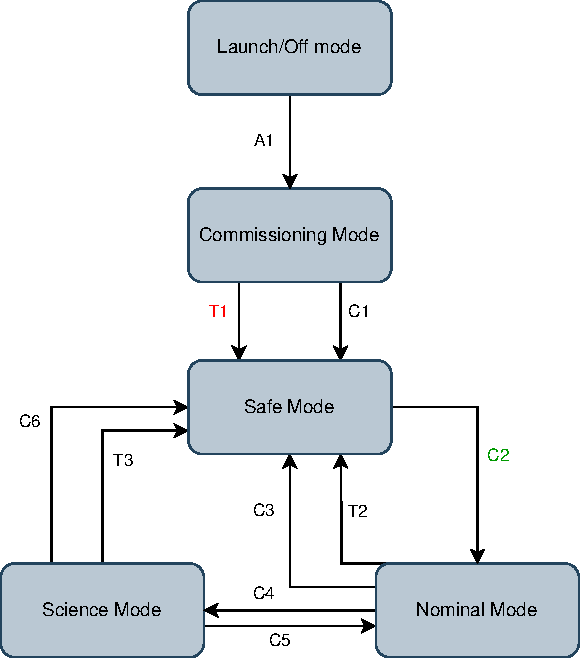
\includegraphics[width=.6\textwidth]{AcubeSAT_System_Modes}
%	\caption[][3cm]{Όλες οι μεταβάσεις μεταξύ των Λειτουργιών Συστήματος}
%	\label{fig:transitions}
%\end{figure}


\subsection{Υποσύστημα Δομής (Structural)}

Το υποσύστημα Structural έχει αναλάβει:
\begin{itemize}
	\item Την ανάλυση και η διαμόρφωση του \ac{COTS} σκελετού 3U (\Cref{fig:structure}) \g{που στεγάζει όλα τα εξαρτήματα του CubeSat και είναι κατασκευασμένος από αλουμίνιο. Οι αναλύσεις δονήσεων είναι ιδιαίτερα σημαντικές, καθώς διερευνούν κατά πόσο ο CubeSat μπορεί να αντέξει τα μηχανικά φορτία κατά την εκτόξευση.}
	\item Τον πλήρη σχεδιασμό, κατασκευή και συναρμολόγηση του \textbf{δοχείου πειράματος} (\Cref{fig:container}).
\end{itemize}

\begin{marginfigure}
	\centering
	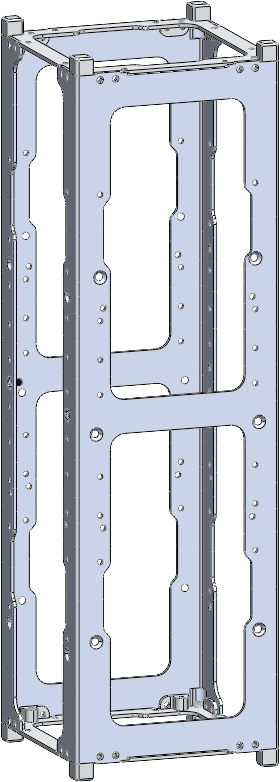
\includegraphics[width=.5\textwidth]{structure}
	\caption{Ο \acs{COTS} σκελετός του CubeSat}
	\label{fig:structure}
\end{marginfigure}

\subsection{Μηχανική Συστήματος (\acs{SYE})}

Η υποομάδα του \acl{SYE} λειτουργεί ως τεχνική αρχή του δορυφόρου. Είναι υπεύθυνη για το συντονισμό των εργασιών και της επικοινωνίας μεταξύ των υποσυστημάτων, τη συμμόρφωση με τα πρότυπα και τις τεχνικές προδιαγραφές, καθώς και τον εντοπισμό \& την επίλυση όλων των ζητημάτων που προκύπτουν από τον πολύπλοκο σχεδιασμό ενός δορυφορικού συστήματος.

Επιπλέον, η ομάδα \ac{SYE} είναι υπεύθυνη για ορισμένα τεχνικά κομμάτια που δεν ανήκουν σε κανένα από τα άλλα υποσυστήματα, όπως την ανάλυση αξιοπιστίας (\acs{RAMS}), την ανάλυση αποτυχιών \& αποτελεσμάτων τους (\ac{FMEA}), την καλωδίωση και το πλάνο κατασκευής \& δοκιμών (\acs{MAIV}).

\subsection{Επιστημονική Μονάδα (\acs{SU})}

Η υποομάδα \acl{SU} είναι υπεύθυνη για τη σχεδίαση και την υλοποίηση του επιστημονικού φορτίου της αποστολής, δηλαδή τη μελέτη της επιδράσεων του περιβάλλοντος Χαμηλής Γήινης Τροχιάς (\ac{LEO}) σε ζυμομύκητες.

\begin{marginfigure}
	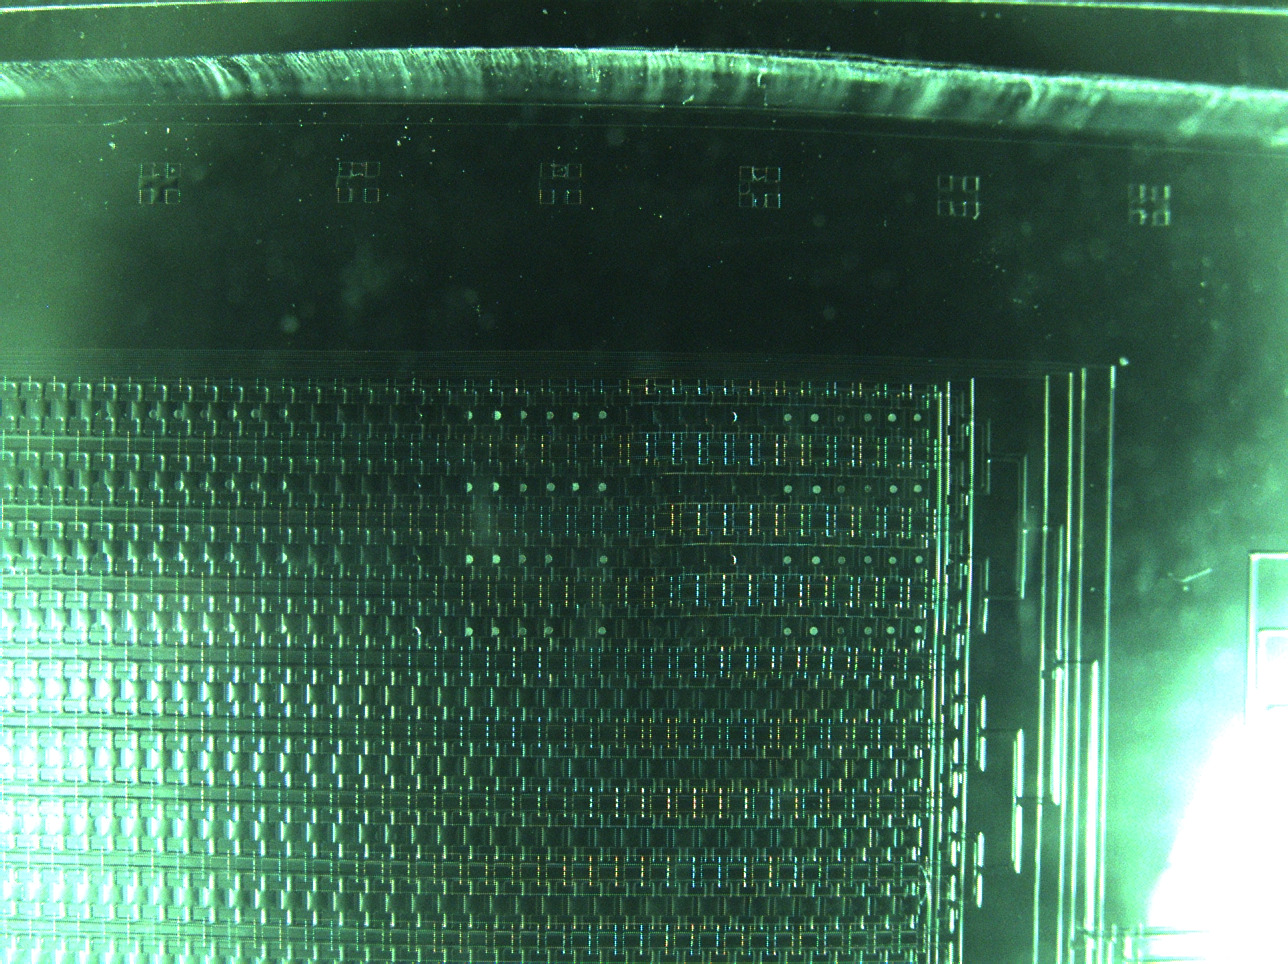
\includegraphics{chipFluor}
	\caption[Παράδειγμα παραγόμενης εικόνας]{Παράδειγμα παραγόμενης εικόνας \autocite{DDJF_PL}}
	\label{fig:chip_fluor}
\end{marginfigure}

Το επιστημονικό φορτίο αποτελείται από τα ακόλουθα λειτουργικά μέρη: \autocite{DDJF_PL}
\begin{compactitem}
	\item Το \textbf{δοχείο πειράματος}, μια δομή αλουμινίου μεγέθους σχεδόν 2U, σε τυπική ατμοσφαιρική πίεση και σχεδιασμένη να φιλοξενεί όλα τα όργανα του πειράματος. Το δοχείο φιλοξενεί επίσης ένα μονόσωμα (\textbf{"unibody"}) που στηρίζει μηχανικά όλα τα εξαρτήματα.
	\begin{marginfigure}
		\centering
		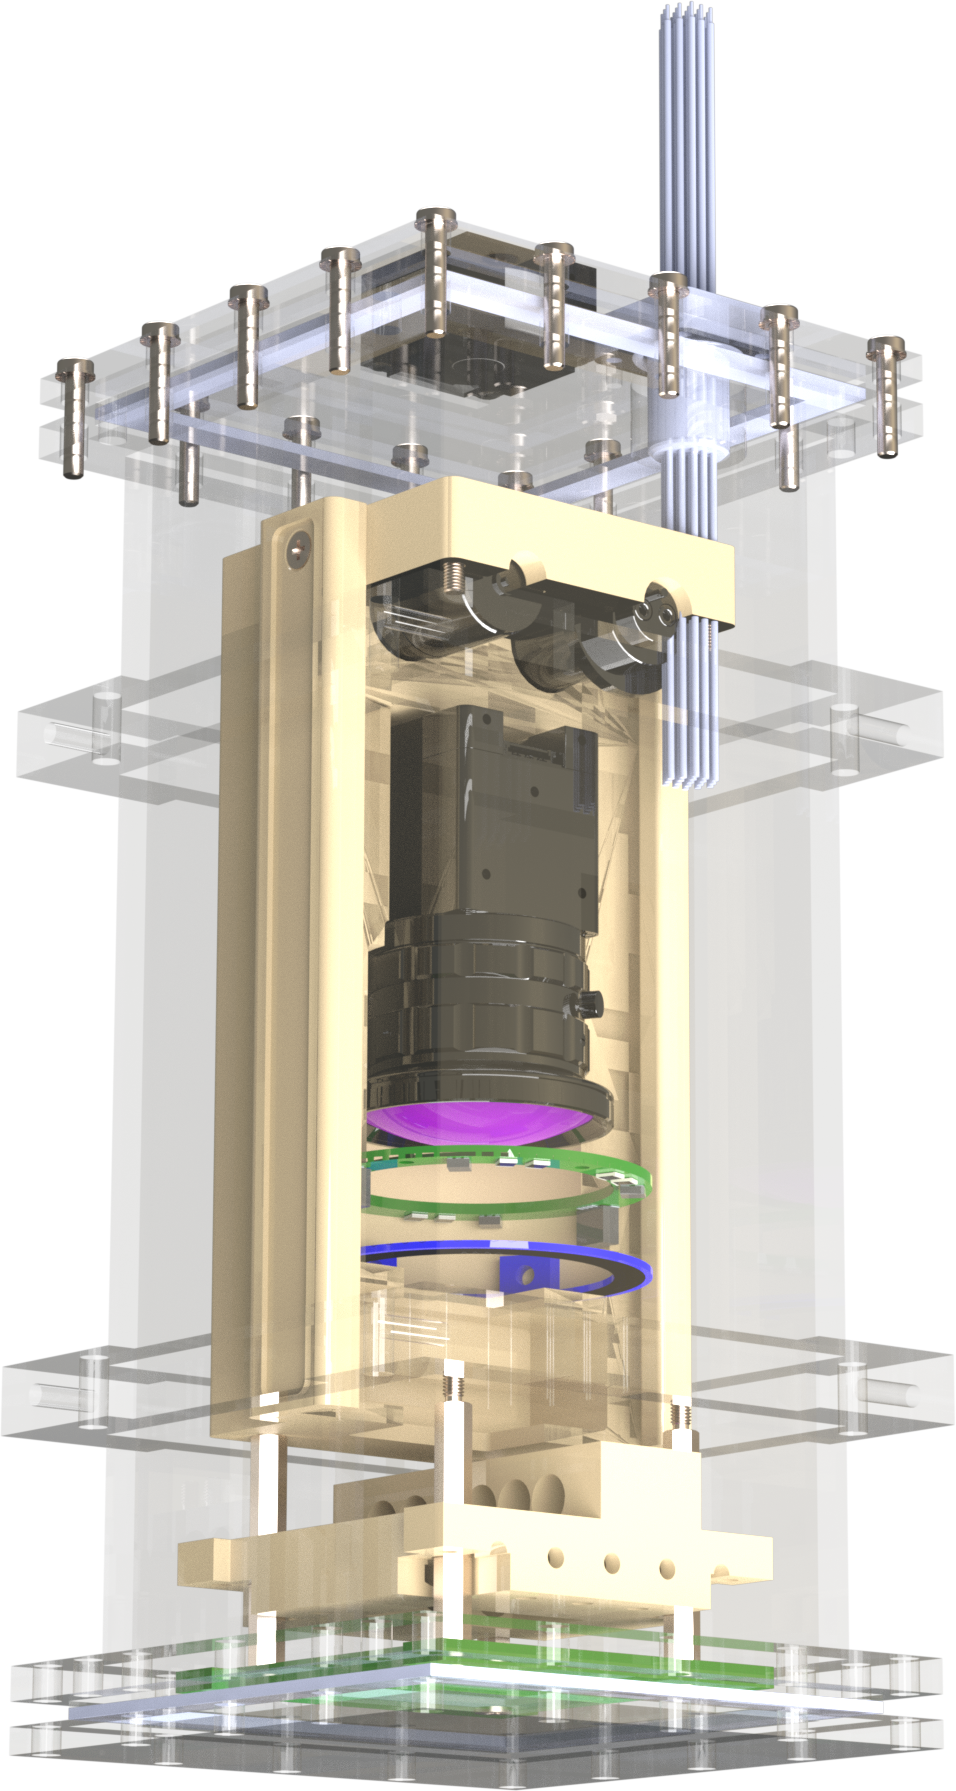
\includegraphics[width=.9\textwidth]{Glass_Payload}
		\caption{Διαφανής προβολή του δοχείου πειράματος και του εσωτερικού του}
		\label{fig:container}
	\end{marginfigure}
	\item Ένα \textbf{τσιπ μικρορευστομηχανικής} (microfluidic chip) βασισμένο στο υλικό \acs{PDMS}, που φιλοξενεί 384 θαλάμους ικανούς να εξετάσουν 190 διαφορετικά στελέχη των μυκητών \emph{Saccharomyces Cerevisiae} για κάθε υποπείραμα.
	\item Ένα \textbf{υδραυλικό σύστημα} που αποτελείται από 2 αντλίες, 14 ηλεκτρικές βαλβίδες και 3 σακούλες υγρών.
	\item Ένα \textbf{οπτικό σύστημα} που λειτουργεί ως μικροσκόπιο, το οποίο περιέχει μια κάμερα και μια σειρά από λαμπτήρες, φίλτρα και ένα φακό
	\item Έναν αριθμό \textbf{θερμαντικών σωμάτων} για τον αυστηρό έλεγχο των θερμοκρασιών λειτουργίας των εξαρτημάτων
	\item Έναν αριθμό πλεοναζόντων \textbf{αισθητήρων} για περιβαλλοντικές μετρήσεις
	\item Μία πλακέτα που περιέχει τον μικροελεγκτή και τα υπόλοιπα εξαρτήματα ελέγχου
\end{compactitem}

\begin{figure}
	\centering
	\caption[Το τσιπ μικρορευστομηχανικής]{Το τσιπ μικρορευστομηχανικής και ο διαχωρισμός του σε 3 επιμέρους υποπειράματα και 1 γραμμή δοκιμής. Οι είσοδοι των υγρών φαίνονται στην αριστερή πλευρά του τσιπ, ενώ οι έξοδοι στα δεξιά. \emph{Πράσινο:} στρώμα ροής. \emph{Μπλε:} στρώμα ελέγχου.}
	\label{fig:chip}
	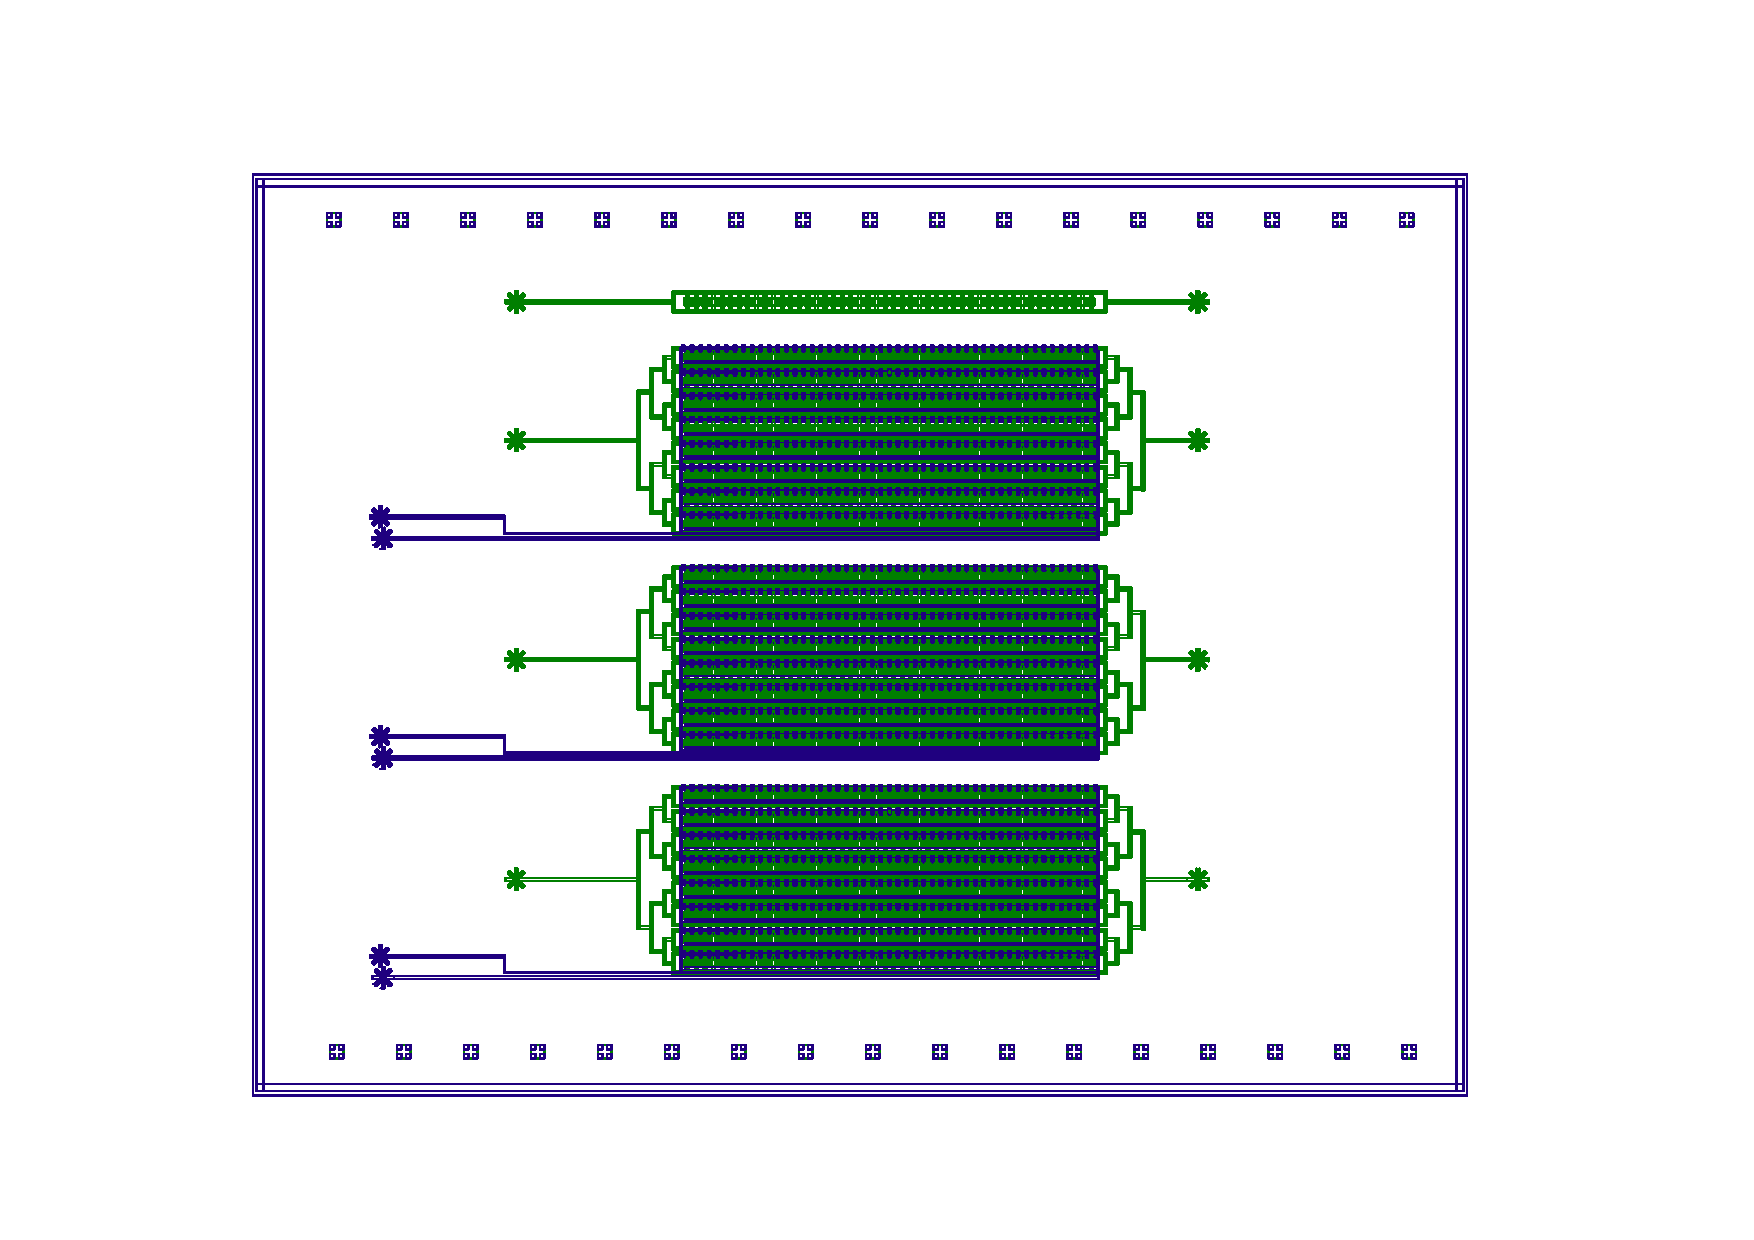
\includegraphics{final_chip.pdf}
	\begin{tikzpicture}[overlay,scale=0.668]
	\draw[very thick,dashed,solarized-base01] (5,10.9) rectangle (-7,11.5) node[below right,scale=.65] {Δοκιμαστική};
	\draw[very thick,dashed,solarized-green] (5,7.85) rectangle (-7,10.8) node[below right] {Υποπείραμα $\alpha$};
	\draw[very thick,dashed,solarized-blue] (5,5) rectangle (-7,7.8) node[below right] {Υποπείραμα $\beta$};
	\draw[very thick,dashed,solarized-red] (5,2) rectangle (-7,4.95) node[below right] {Υποπείραμα $\gamma$};
	\end{tikzpicture}
	\setfloatalignment{b}
\end{figure}

Το πείραμα επιβάλλει κάποιους περιορισμούς στο σχεδιασμό του \ac{FDIR}:
\phantomsection\label{sec:su_fdir}
\begin{enumerate}
	\item \textbf{Διακοπή} \g{ενός από τα τρία 72ωρα υποπειράματα κατά τη διάρκεια της εκτέλεσης μπορεί να σημαίνει πλήρη απώλεια του υποπειράματος. Ο αντίκτυπος ενός τέτοιου γεγονότος εξαρτάται από τη διάρκεια και τη χρονική στιγμή της εμφάνισής του. Σε κάθε περίπτωση, επαρκής παρατηρησιμότητα θα επιτρέψει στο επίγειο πείραμα να μιμηθεί όσο το δυνατόν περισσότερο τις συνθήκες εντός τροχιάς.}
	\item \textbf{Το πάγωμα} των υγρών στο εσωτερικό του τσιπ και των σωλήνων μπορεί να οδηγήσει σε μόνιμη βλάβη της διάταξης. Ως εκ τούτου, μπορεί να απαιτηθεί η ενεργή θέρμανση ακόμη και κατά τη διάρκεια της ασφαλούς λειτουργίας, μετά την εκτέλεση του πρώτου υπο-πειράματος και την εισροή υγρού στο σύστημα. Αυτά τα χαρακτηριστικά επιβάλλουν περαιτέρω περιορισμούς στην ελάχιστη διαθεσιμότητα του συστήματος, ανάλογα με τις περιβαλλοντικές συνθήκες.
\end{enumerate}

\subsection{Υποσύστημα Θερμικού Ελέγχου (Thermal)}


Η υποομάδα Thermal είναι υπεύθυνη για τη θερμική ανάλυση του δορυφόρου, όπου η εισερχόμενη ηλιακή ακτινοβολία συνδυάζεται με την απαγωγή θερμότητας των υποσυστημάτων, με σκοπό τον προσδιορισμό των χειρότερων θερμοκρασιών που αντιμετωπίζει ο δορυφόρος, σε θερμές και ψυχρές συνθήκες.

Τα αποτελέσματα της θερμικής ανάλυσης οδηγούν συνήθως στην εφαρμογή παθητικών ή ενεργητικών μεθόδων θερμικού ελέγχου. Ειδικότερα στο AcubeSAT, χρησιμοποιούνται 3 ηλεκτρονικά ελεγχόμενα θερμαντικά σώματα για τις μπαταρίες, το πειραματικό τσιπ και τις βαλβίδες.

\subsection{Ανάλυση Τροχιάς (Trajectory)}

Η υποομάδα Trajectory είναι υπεύθυνη για την ανάλυση της τροχιάς του διαστημικού σκάφους, την αποτίμηση των επιπτώσεων της ακτινοβολίας, τη συμμόρφωση του δορυφόρου με τους κανονισμούς για τα διαστημικά σκουπίδια και την εκτίμηση της διάρκειας ζωής του σε τροχιά.

\begin{figure}
	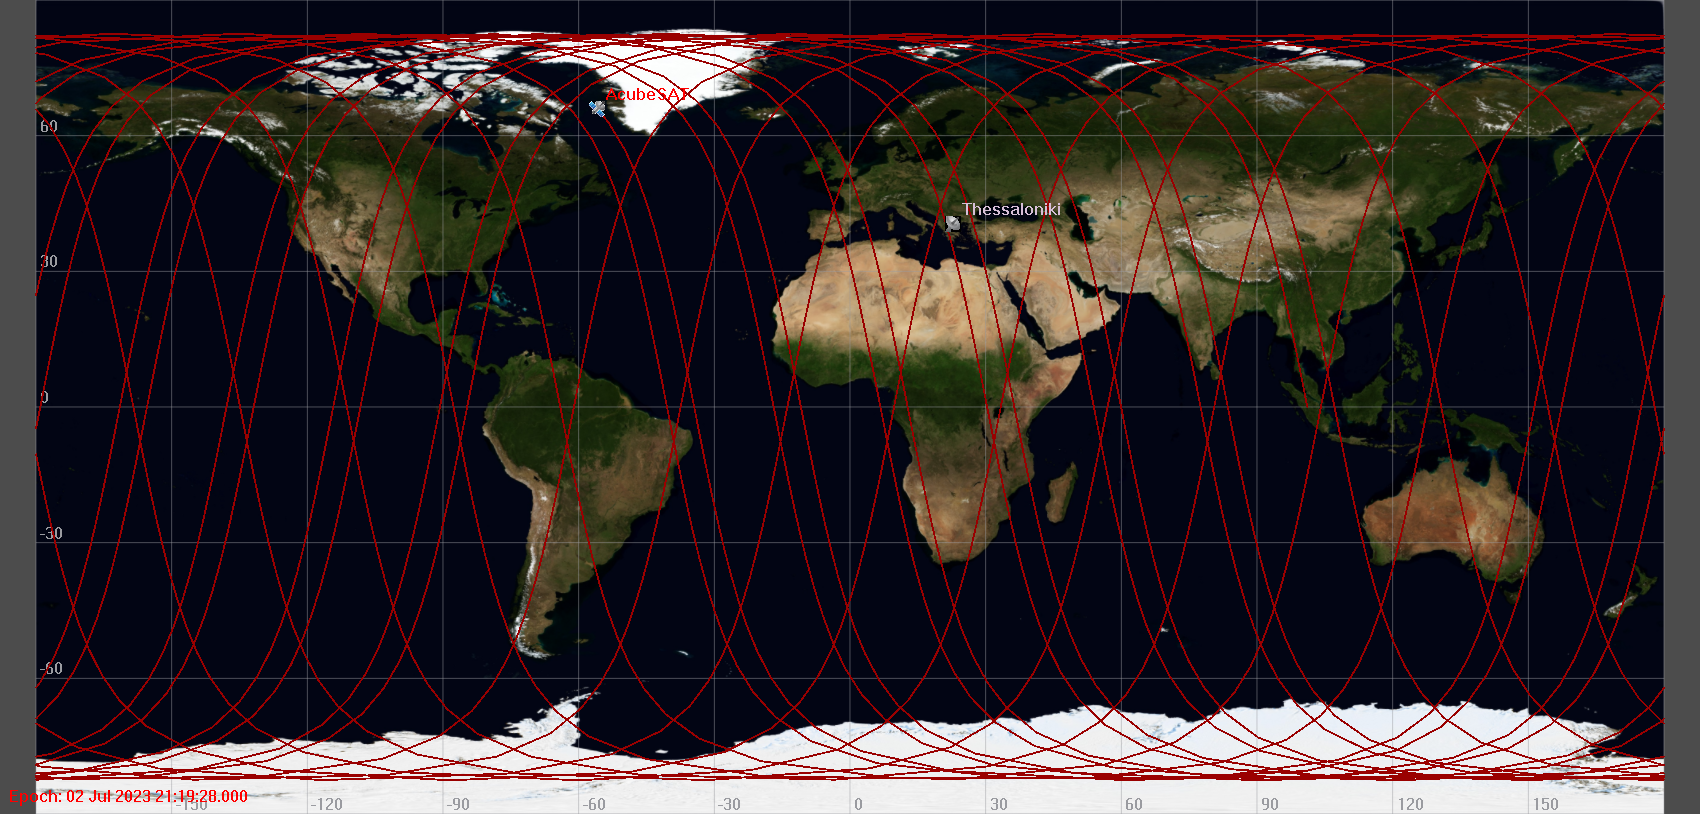
\includegraphics{GmatScreenShot_002}
	\caption[Επίγειο ίχνος μιας πιθανής τροχιάς του AcubeSAT]{Επίγειο ίχνος μιας πιθανής τροχιάς του AcubeSAT, σχεδιασμένο με χρήση του εργαλείου \acl{GMAT} της NASA}
	\label{fig:gmat}
\end{figure}

\g{Οι απαιτήσεις του AcubeSAT δεν υπαγορεύουν τη χρήση προωθητήρων, πράγμα που σημαίνει ότι η τροχιά του δορυφόρου καθορίζεται αποκλειστικά από την εκτόξευση και δεν μπορεί να τροποποιηθεί κατά την πτήση. Καθώς πληροφορίες για την εκτόξευση είναι άγνωστες μέχρι κάποιο χρονικό διάστημα πριν από την παράδοση του δορυφόρου, εκτελείται ένα σύνολο αναλύσεων ευαισθησίας για τον προσδιορισμό των επιτρεπόμενων τροχιών} \autocite{MDO,anthopoulos_orbital_analysis_2020}.

% Maybe add some info about the sensitivity results and LTAN value?
% No

\section{Χρησιμοποιούμενα εργαλεία}

Ως ένα περίπλοκο πρότζεκτ, το AcubeSAT χρησιμοποιεί ένα σύνολο βοηθητικών εργαλειών, έτοιμων ή κατασκευασμένων στην ομάδα, για την εκπλήρωση των τεχνικών και οργανωτικών εργασιών του. Ενδεικτικά παραθέτουμε τα:
\begin{compactitem}
	\item \foothref{https://gitlab.com/acubesat}{GitLab}, για διαμοιρασμό κώδικα αλλά και οργάνωση εργασιών \& καθηκόντων
	\item \foothref{https://ocdt.esa.int/}{Open Concurrent Design Tool}, μία πλατφόρμα για διαμοιρασμό τεχνικών δεδομένων και τιμών για τα εξαρτήματα του δορυφόρου
	\item  \foothref{https://www.latex-project.org/}{\LaTeX} και \foothref{https://www.overleaf.com/}{Overleaf}, για συγγραφή της τεχνικής βιβλιογραφίας και τεκμηρίωσης
	\item \foothref{https://acubesat.spacedot.gr/requirements-tree}{Requirements Tree}, μία διαδραστική προβολή των τεχνικών προδιαγραφών του δορυφόρου
	\item \foothref{https://gitlab.com/acubesat/utilities/mattermost-documentation-bot}{Documentation List}, \g{πλατφόρμα για καταλογοποίηση και πλοήγηση στα έγγραφα που έχει παράξει η ομάδα}
\end{compactitem}

\chapter{Η φιλοσοφία \acs{FDIR} της πρωτοβουλίας SAVOIR}
\label{cap:savoir}

Στην παρούσα ενότητα θα εξετάσουμε συνοπτικά τον συνδυασμό δύο φιλοσοφιών που χρησιμοποιούνται από ευρωπαϊκούς φορείς με δράση στο χώρο του διαστήματος. Η πρώτη φιλοσοφία συνδέεται με το \textbf{πρότυπο \texttt{ECSS-E-ST-70-41C}} \autocite{ECSS-E-ST-70-41C} του οργανισμού \acf{ECSS}, το οποίο ορίζει το βασικό σύνολο τηλεμετρίας (\acs{TM}) και τηλεεντολών (\acs{TC}) που χρειάζεται η πλατφόρμα ενός δορυφόρου για να ελεγθεί από τον σταθμό βάσης.

Η δεύτερη φιλοσοφία βασίζεται στο εγχειρίδιο \textbf{\texttt{SAVOIR-HB-003} "\citetitle{SAVOIR-HB-003}"} \autocite{SAVOIR-HB-003} της πρωτοβουλίας \textbf{\acf{SAVOIR}}. Το εγχειρίδιο αυτό βασίζεται στις λειτουργίες του προτύπου \texttt{ECSS-E-ST-70-41C}, και προτείνει μία λεπτομερή μεθοδολογία για την ανάπτυξη του \ac{FDIR} σε ένα διαστημικό πρότζεκτ. Το εγχειρίδιο είναι η βάση της φιλοσοφίας που ακολουθείται στη συνέχεια της εργασίας.

\section{Το Πρότυπο Αξιοποίησης Πακέτων \acs{ECSS}}
\label{sec:pus}


Το πρότυπο \texttt{ECSS-E-ST-70-41C}, ή εν συντομία \textbf{\acs{PUS}} (\acl{PUS}) ορίζει ένα σύνολο από δομημένες \textbf{τηλεεντολές} και \textbf{τηλεμετρία} που μπορεί να χρησιμοποιήσει ένα διαστημικό σκάφος για να επικοινωνήσει με τη γη. Μπορεί να παρομοιαστεί με μία "γλώσσα" που χρησιμοποιεί ένα σύστημα ώστε οι χειριστές να έχουν πλήρη επίγνωση και πλήρη έλεγχο των λειτουργιών του. Ταυτόχρονα, ορίζει τις βασικές λειτουργίες που πρέπει να πραγματοποιεί ένα αυτόνομο σύστημα με αυστηρούς όρους, και καθορίζει τις έννοιες των \textbf{εφαρμογών}, των \textbf{παραμέτρων} και των \textbf{γεγονότων}.

\begin{marginfigure}
	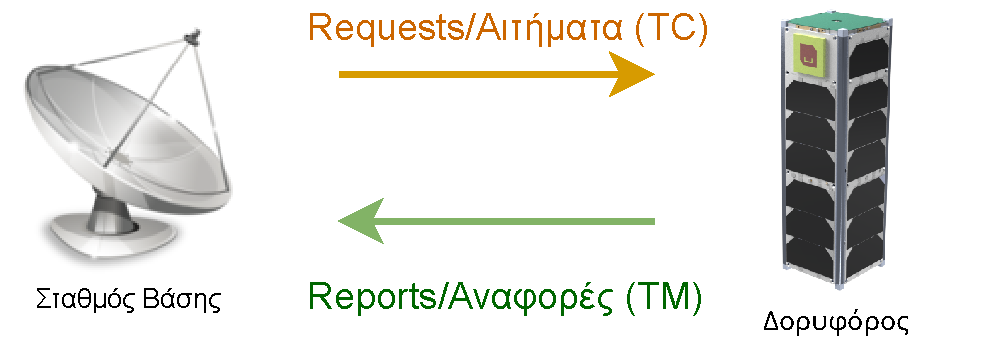
\includegraphics{ECSS-rq-el}
	\caption[]{Το μοντέλο μεταφοράς δεδομένων του \ac{PUS}}
	\label{fig:pusmodel}
\end{marginfigure}

Το πρότυπο αυτό μπορεί να χρησιμοποιηθεί σε οποιαδήποτε διαστημική αποστολή, και από τους συγγραφείς του συνιστάται η προσαρμογή και επιλογή των πιο χρήσιμων "υπηρεσιών" (\textbf{services}) \g{από αυτές που προσφέρει. Συνοπτικά, παρέχει τις εξής 20 υπηρεσίες:} \autocite{ECSS-E-ST-70-41C,ECSS-E-70-41A,kaufeler_esa_standard_1994}

\marginnote{
	\item \textbf{Εφαρμογή} (application process): Κάθε οντότητα (υλικού ή λογισμικού) που μπορεί να λάβει τηλεεντολές και να παράγει τηλεμετρία
	
	\item \textbf{Γεγονός} (events): Αξιοσημείωτο συμβάν που λαμβάνει χώρα στο δορυφόρο, όπως:
	\begin{compactitem}
		\item Αυτόνομη ενέργεια
		\item Ανιχνευμένη βλάβη ή ανωμαλία
		\item Προκαθορισμένο βήμα μιας διαδικασίας
	\end{compactitem}

	\item \textbf{Παράμετρος} (parameter): Μεταβλητός και αναγνώσιμος περιέκτης δεδομένων που μπορεί να αντιπροσωπεύει:
	\begin{itemize}
		\item Βασικές ρυθμίσεις του συστήματος ή άλλων στοιχείων
		\item Μετρήσεις αισθητήρων και άλλες τιμές τηλεμετρίας
		\item Αποτελέσματα και διαγνωστικά του \ac{FDIR}
	\end{itemize}

%	\item \textbf{Μήνυμα} (message): 
}

\begin{compactitem}
	\item \textbf{\texttt{ST[01]}: Request verification}
	
	Παρέχει αναφορές επιβεβαίωσης ή αποτυχίας για εκτελούμενες εντολές. Αυτή η υπηρεσία ουσιαστικά ενημερώνει τους χειριστές για την (επιτυχημένη ή μη) κατάσταση των \ac{TC} που αποστέλλονται στον δορυφόρο.
	
	\item \textbf{\texttt{ST[02]}: Device access}
	
	Επιτρέπει την ενεργοποίηση, τον έλεγο και τη ρύθμιση των περιφερειακών συσκευών που βασίζονται σε απλά πρωτόκολλα επικοινωνίας.
	
	\item \textbf{\texttt{ST[03]}: Housekeeping}
		
		Παράγει περιοδικές αναφορές που περιέχουν τιμές παραμέτρων. Η υπηρεσία αυτή ουσιαστικά συνθέτει τους περιοδικούς ραδιοφάρους (\textbf{\acs{RF} beacons}) του δορυφόρου, χωρίς προηγούμενο ερέθισμα.
		
		\item \textbf{\texttt{ST[04]}: Parameter statistics reporting}
		
		Επιτρέπει την αναφορά στατιστικών στοιχείων (ελάχιστο, μέγιστο, μέσος όρος, τυπική απόκλιση) για παραμέτρους σε καθορισμένα χρονικά διαστήματα.
		
		\item \textbf{\texttt{ST[05]}: Event reporting}
		
		Ενημερώνει τους χειριστές όταν λαμβάνουν χώρα γεγονότα.
		
		\item \textbf{\texttt{ST[06]}: Memory management}
		
		\g{Επιτρέπει την απευθείας ανάγνωση και εγγραφή σε μονάδες μνήμης. Αυτό μπορεί να είναι χρήσιμο για σκοπούς αποσφαλμάτωσης, ανάκτησης δεδομένων της αποστολής, ή φόρτωσης εντελώς νέου λογισμικού. Η υπηρεσία παρέχει επίσης τη δυνατότητα κατεβάσματος και ανεβάσματος αρχείων σε ένα σύστημα αρχείων.}
		
		\item \textbf{\texttt{ST[07]}: Task management} \emph{(καταργημένη)}
		
		Επιτρέπει τη διακοπή, την αναστολή ή την επανάληψη διεργασιών σε περίπτωση έκτακτης ανάγκης. Η υπηρεσία αυτή έχει αφαιρεθεί από το πρότυπο και παρατίθεται για ιστορικούς λόγους.
		
		\item \textbf{\texttt{ST[08]}: Function management}
		
		Παρέχει τη δυνατότητα εκτέλεσης προκαθορισμένων ενεργειών που μπορούν να λάβουν περαιτέρω παραμέτρους. Οι ενέργειες αυτές μπορεί να αντιστοιχούν σε πειραματικές διαδικασίες ή γενικότερες λειτουργίες.
		
		\item \textbf{\texttt{ST[09]}: Time management}
		
		Επιτρέπει την περιοδική αναφορά της τιμής του ρολογιού του CubeSat, για σκοπούς παρατηρησιμότητας και συσχέτισης.
		
		\item \textbf{\texttt{ST[10]}: Time packet} \emph{(καταργημένο)}
		
		Χρησιμοποιήθηκε στο παρελθόν για την παροχή πληροφοριών ρολογιού. Η υπηρεσία αυτή έχει αφαιρεθεί από το πρότυπο και παρατίθεται για ιστορικούς λόγους.
		
		\item \textbf{\texttt{ST[11]}: Time-based scheduling}
		
		Επιτρέπει στους χειριστές να προγραμματίζουν ("time-tag") \g{τηλεεντολές για εκτέλεση σε μελλοντικές χρονικές στιγμές, αντί για αμέσως.}
		
		\item \textbf{\texttt{ST[12]}: On-board monitoring}
		
		Επιτρέπει τον έλεγχο των τιμών των παραμέτρων για να διασφαλιστεί ότι παραμένουν εντός ρυθμιζόμενων ορίων. Κάθε φορά που τα όρια παραβιάζονται, δημιουργείται ένα γεγονός (\texttt{ST[05]}) για περαιτέρω επεξεργασία.
		
		\item \textbf{\texttt{ST[13]}: Large packet transfer}
		
		Παρέχει μια μέθοδο τμηματοποίησης (segmentation) μηνυμάτων, για συμβολοσειρές που είναι πολύ μεγάλες για να χωρέσουν στο μέγιστο επιτρεπόμενο μήκος για \ac{TC} ή \ac{TM}.
		
		\item \textbf{\texttt{ST[14]}: Real-time forwarding control}
		
		Αυτή η υπηρεσία είναι υπεύθυνη για τον έλεγχο της παραγόμενης τηλεμετρίας που εκπέμπεται άμεσα προς το Σταθμό Βάσης.
		
		\item \textbf{\texttt{ST[15]}: On-board storage and retrieval}
		
		Επιτρέπει την αποθήκευση των παραγόμενων αναφορών, καθώς και την ανάκτησή τους όταν ο δορυφόρος περνάει επάνω από το Σταθμό Βάσης.
		
		\item \textbf{\texttt{ST[16]}: On-board traffic management} \emph{(deprecated)}
		
		Επιτρέπει την παρακολούθηση της κατάστασης και του φόρτου ενός διαύλου δεδομένων. Η υπηρεσία αυτή έχει αφαιρεθεί από το πρότυπο και παρατίθεται για ιστορικούς λόγους.
		
		\item \textbf{\texttt{ST[17]}: Test}
		
		Η υπηρεσία αυτή παρέχει απλές εντολές για ελέγχους υγείας του δορυφόρου.
		
		\item \textbf{\texttt{ST[18]}: On-board operations procedure}
		
		Επιτρέπει τη φόρτωση, τον έλεγχο (εκκίνηση, αναστολή, συνέχιση, διακοπή) και τη ρύθμιση των "operations procedures", δλδ. ακολουθιών εντολών σε κάποια ερμηνευμένη γλώσσα προγραμματισμού.
		
		\item \textbf{\texttt{ST[19]}: Event-action}
		
		Παρέχει τη δυνατότητα αυτόνομης εκτέλεσης \acp{TC} όταν λαμβάνει χώρα ένα συμβάν \texttt{ST[05]}.
		
		\item \textbf{\texttt{ST[20]}: On-board parameter management}
		
		\g{Παρέχει τη δυνατότητα ανάγνωσης και αλλαγής τιμών των παραμέτρων του δορυφόρου.}
		
		\item \textbf{\texttt{ST[21]}: Request sequencing}
		
		Επιτρέπει στους χειριστές να φορτώνουν \acp{TC} για να εκτελεστούν με διαδοχική σειρά.
		
		\item \textbf{\texttt{ST[22]}: Position-based scheduling}
		
		Παρέχει τη δυνατότητα εκτέλεσης \ac{TC} σε συγκεκριμένα σημεία της τροχιάς.
		
		\item \textbf{\texttt{ST[23]}: File management}
		
		Επιτρέπει την εκτέλεση διαχειριστικών εντολών σε συστήματα αρχείων στον δορυφόρο, όπως \emph{αντιγραφή}, \emph{μετακίνηση}, \emph{διαγραφή}, ή \emph{κλείδωμα}.
\end{compactitem}

\section{Το Εγχειρίδιο \acs{FDIR} του \acs{SAVOIR}}

Το εγχειρίδιο \texttt{SAVOIR-HB-003} \g{περιγράφει με λεπτομέρεια τη διαδικασία και μεθοδολογίες για εφαρμογή του \acs{FDIR}, βασισμένο σε αποτελέσματα \& διδάγματα από προηγούμενες ευρωπαϊκές αποστολές. Σε αυτό το κεφάλαιο θα σχολιαστούν τα κομμάτια που αφορούν μία αποστολή} CubeSat χαμηλού κόστους.

\subsection{Βήματα σχεδιασμού \acs{FDIR}}
Το εγχειρίδιο αναλύει τα βήματα του σχεδιασμού του \acs{FDIR}, άρρηκτα συνδεδεμένα με τις φάσεις μιας τυπικής διαστημικής αποστολής. Έχει σημασία να τονιστεί πως ο σχεδιασμός του \acs{FDIR} ξεκινάει πριν την υλοποίηση και επαλήθευσή του, από γενικό σε πιο λεπτομερές επίπεδο. Αυτή η λογική "καταρράκτη" που ακολουθείται από τα διαστημικά πρότζεκτ αντιτίθεται στην πιο σύγχρονη και ευέλικτη "agile" λογική των πρότζεκτ μικρού βεληνεκούς. Παρ' όλα αυτά, οι ιδέες του εγχειριδίου μπορούν να εφαρμοστούν σε οποιαδήποτε λογική ανάπτυξης ενός πρότζεκτ.

Τα βήματα της διαδικασίας \acs{FDIR} ορίζονται ως τα εξής:
\begin{enumerate}
	\setcounter{enumi}{-1}
	\item \textbf{Τεχνικές προδιαγραφές} (requirements): \g{Εδώ, με βάση τις απαιτήσεις της κάθε αποστολής, αναλύονται αντίστοιχα οι απαιτήσεις του συστήματος για αξιοπιστία \& διαθεσιμότητα, και εξάγονται οι βασικές προδιαγραφές για το σύστημα} \acs{FDIR}. Σε αυτό το στάδιο δεν λαμβάνονται σχεδιαστικές αποφάσεις και δεν επιλέγονται λύσεις, αλλά καθορίζονται τα προβλήματα που πρέπει να λυθούν και τα βασικά κριτήρια επιτυχίας του συστήματος.
	\label{itm:fdir_reqs}
	
	Αν και η διατύπωση τεχνικών προδιαγραφών σε τυχαία γεγονότα και βλάβες για τις οποίες δεν υπάρχει αρκετή διαθέσιμη πληροφορία είναι δύσκολη, το εγχειρίδιο προτείνει ένα σύνολο από τεχνικές προδιαγραφές \autocite[42]{SAVOIR-HB-003} που μπορούν να χρησιμοποιηθούν από αποστολές. Ένα μεγάλο σύνολο των προδιαγραφών αυτών καλύπτεται και από τη σχεδίαση που παρουσιάζουμε στις επόμενες ενότητες.
	\item \textbf{Ορισμός ιδέας} (concept): Εδώ γίνεται σύγκριση των διαθέσιμων γενικών στρατηγικών του \acs{FDIR} που θα πληρούν τις προδιαγραφές του \cref{itm:fdir_reqs}. Αναλύονται λύσεις όπως πλεονασμός, διασταυρωμένες συνδέσεις, συστήματα τριπλής ψηφοφορίας ή εγγενώς αξιόπιστα (και υψηλού κόστους) εξαρτήματα.
	\label{itm:fdir_concept}
	\item \textbf{Ορισμός αρχιτεκτονικής} (architecture): Σε αυτό το βήμα ορίζεται σε ένα γενικό επίπεδο ο τρόπος λειτουργίας του \acs{FDIR} με βάση τις δυνατότητες του συστήματος, χωρίς τις λεπτομέρειες υλοποίησης αλλά με αρκετή πληροφορία για τη δομή του συστήματος και τις διεπαφές των στοιχείων του.
	\item \textbf{Λεπτομερής σχεδιασμός} (detailed design): Προτού ολοκληρωθεί ο πλήρης σχεδιασμός του \acs{FDIR}, απαιτείται η κατάστρωση του \textbf{\acf{FMEA}} \autocite{carlson_effective_fmeas_2012} για το σύστημα και τα υποσυστήματα. Το \acs{FMEA} πρόκειται για τον \textbf{κατάλογο όλων των πιθανών αποτυχιών} για ένα εξάρτημα του δορυφόρου, όπου καταλογοποιούνται με δομημένο τρόπο οι πιθανές βλάβες και η σοβαρότητά τους.
	
	Στη συνέχεια, για κάθε σημαντικό αντικείμενο του καταλόγου \acs{FMEA} αναλύεται το \textbf{\acf{HSIA}} \autocite{ECSS-Q-ST-30-02C}. Πρακτικά, για κάθε βλάβη ορίζονται σε όρους λογισμικού τα \textbf{παρακολουθούμενα δεδομένα} και οι \textbf{ενέργειες απομόνωσης \& επιδιόρθωσης}.
	
	Πέρα από τα παραπάνω, διατυπώνεται ο ακριβής τρόπος και η ροή λειτουργίας του \acs{FDIR} για κάθε λειτουργία του δορυφόρου, με ιδιαίτερη έμφαση στην Ασφαλή Λειτουργία (\Cref{itm:safe_mode}).
	\label{itm:fdir_cdr}
	\item \textbf{Υλοποίηση \& επαλήθευση}: Σε αυτό το στάδιο κατασκευάζεται το υλικό και συγγράφεται το λογισμικό που εκτελούν το \acs{FDIR}. Ακόμα, για τα αντικείμενα της λίστας \acs{HSIA}, πραγματοποιείται \textbf{επαλήθευση} μέσω ανάλυσης ή δοκιμής. Πιο συγκεκριμένα, πρέπει να προσομοιωθεί ή κάθε επίφοβη αποτυχία (feared event), και να επαληθευθεί πως το σύστημα μπορεί να την αντιμετωπίσει με αναμενόμενο τρόπο.
	\label{itm:fdir_valid}
	\item \textbf{Επικύρωση} (validation): Σε αυτό το στάδιο πραγματοποιούνται δοκιμές του \acs{FDIR} σε επίπεδο συστήματος, ως μέρος της δοκιμαστικής καμπάνιας\footnote{Μπορεί να περιέχει τις λειτουργικές δοκιμές συστήματος (ambient tests), ή τις δοκιμές περιβάλλοντος (environmental tests) όπου προσομοιώνονται συνθήκες διαστήματος} ολόκληρης της αποστολής, και πραγματοποιούνται οι τελικές μικρορυθμίσεις.
	\item \textbf{Προετοιμασία για χειρισμό} (operations preparation): \g{Στο τελευταίο βήμα πραγματοποιούνται οι τελικές αλλαγές στη βιβλιογραφία \& τεκμηρίωση για τον απομακρυσμένο χειρισμό της αποστολής.}
\end{enumerate}

\g{Αν και όλα τα παραπάνω βήματα έχουν σημασία, για "λιτές" αποστολές πρέπει να εστιαστεί προσοχή στις τεχνικές προδιαγραφές (\Cref{itm:fdir_reqs}), στον ορισμό ιδέας (\Cref{itm:fdir_concept}), στον λεπτομερή σχεδιασμό (\Cref{itm:fdir_cdr}) και στην επαλήθευση (\Cref{itm:fdir_valid}). Ένα παράδειγμα εφαρμογής της παραπάνω διαδικασίας βρίσκεται στο \Cref{cap:practical}.}

Σε αυτό το σημείο θα πρέπει να τονιστεί πως η διαδικασία σχεδιασμού του \acs{FDIR} και γενικότερα της μελέτης αξιοπιστίας του συστήματος είναι κάτι που πρέπει να λαμβάνεται υπ' όψιν καθ' όλη τη διάρκεια σχεδιασμού ενός διαστημικού συστήματος, και όχι μόνο στον λεπτομερή σχεδιασμό ή στην επαλήθευση. Ο τομέας του \acf{RAMS} συνδέεται άμεσα με όλα τα υπόλοιπα υποσυστήματα, λαμβάνοντας τις απαραίτητες εισόδους αλλά και επηρεάζοντας σε μεγάλο βαθμό το σχεδιασμό. Ειδικότερα σε νέα CubeSat projects, ο τομέας της αξιοπιστίας τείνει να μη λαμβάνει τη δέουσα σημασία \autocite{langer_reliability_estimation_2017}.

\subsection{Προτεινόμενη αρχιτεκτονική}

Το εγχειρίδιο προτείνει κάποιες αρχές για την αρχιτεκτονική ενός συστήματος \acs{FDIR}, η πρώτη από τις οποίες το εξετάζει ως ένα \textbf{ιεραρχικό} σύστημα, όπου μικρής σημασίας αποτυχίες ξεκινούν από \textbf{εσωτερικά εξαρτήματα} και διορθώνονται σε επίπεδο εξαρτήματος, ή διαδίδονται στο υπόλοιπο σύστημα και απαιτούν σημαντικότερες ενέργειες ανάκαμψης (\Cref{fig:FDIR-levels}).

\begin{figure}
	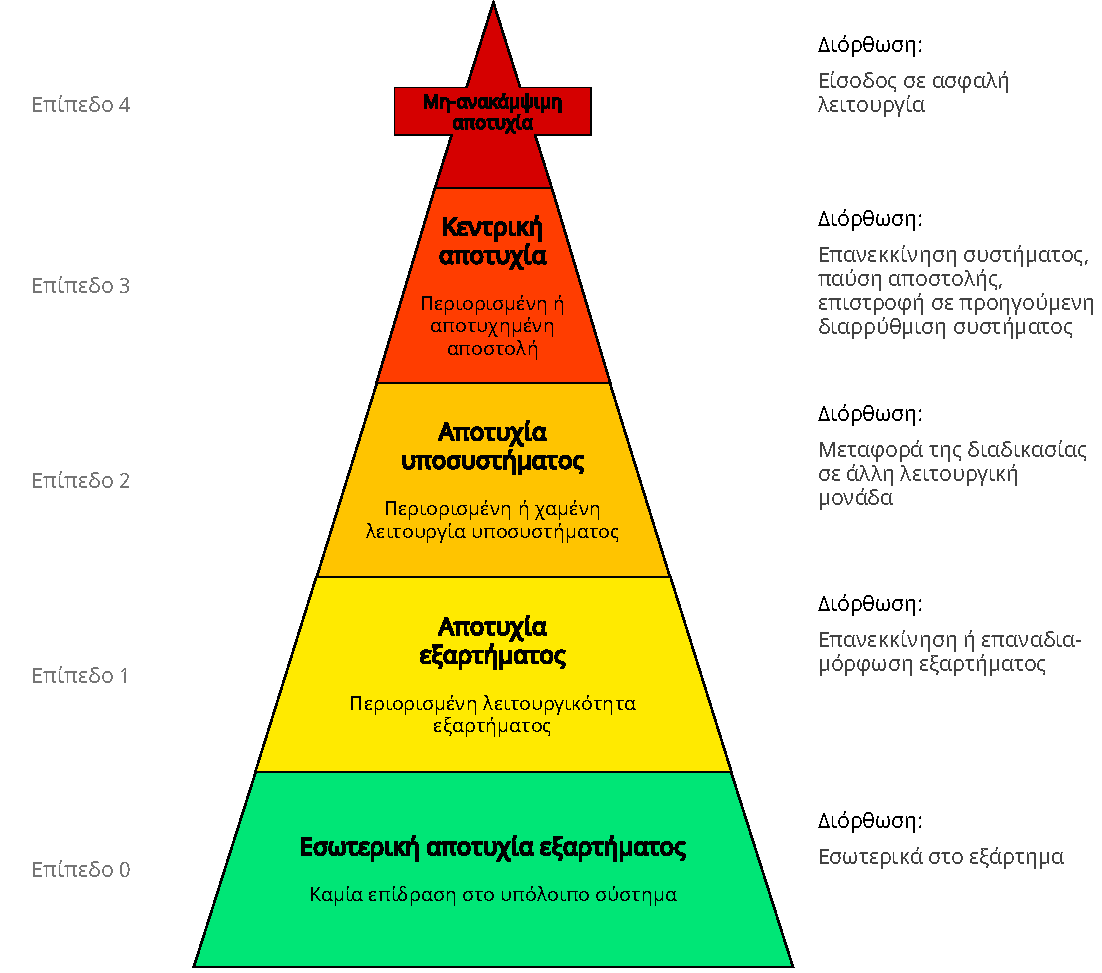
\includegraphics{FDIR-levels}
	\caption[Προτεινόμενη ιεραρχία των διαφορετικών επιπέδων FDIR από το SAVOIR]{Προτεινόμενη ιεραρχία των διαφορετικών επιπέδων \acs{FDIR} από το \acs{SAVOIR}. Η κάθε αποστολή μπορεί να επιλέξει διαφορετικά επίπεδα για να απλοποιήσει την υλοποίηση του συστήματος.}
	\label{fig:FDIR-levels}
\end{figure}

\g{Συνεχίζοντας, παρουσιάζεται μία \textbf{προσαρμόσιμη} υλοποίηση που εκμεταλλεύεται τη \textbf{βάση δεδομένων} του συστήματος και την επικοινωνία με τα} \textbf{\acs{PUS} services} \g{ώστε να καλυφθούν πλήρως οι ανάγκες του \acs{FDIR}. Η λογική αυτή προϋποθέτει τα ακόλουθα:}
\begin{compactenum}
	\item \g{Δεδομένα αξιοπιστίας αποθηκεύονται σε \textbf{παραμέτρους} (π.χ. τιμές αισθητήρων, κατάσταση περιφερειακών)}
	\item \g{Οι παράμετροι αυτές \textbf{παρακολουθούνται} από την υπηρεσία} on-board monitoring. \g{Όταν κάποια παράμετρος αποκτήσει τιμή εκτός ορίων, σημαίνει πως έχει εμφανιστεί κάποια αποτυχία.}
	\item \g{Κάθε έξοδος από τα όρια δημιουργεί ένα \textbf{γεγονός} που τηλεμετράται} (\acs{TM}) \g{στους χειριστές.}
	\item \g{Κάθε γεγονός είναι συνδεδεμένο με μία \textbf{αντίδραση}, αποθηκευμένη στην υπηρεσία} event-action.
	\item \g{Η αντίδραση αυτή μπορεί να είναι μία ή περισσότερες \textbf{διαδικασίες} που διορθώνουν την βλάβη.}
\end{compactenum}

\begin{figure*}[h]
	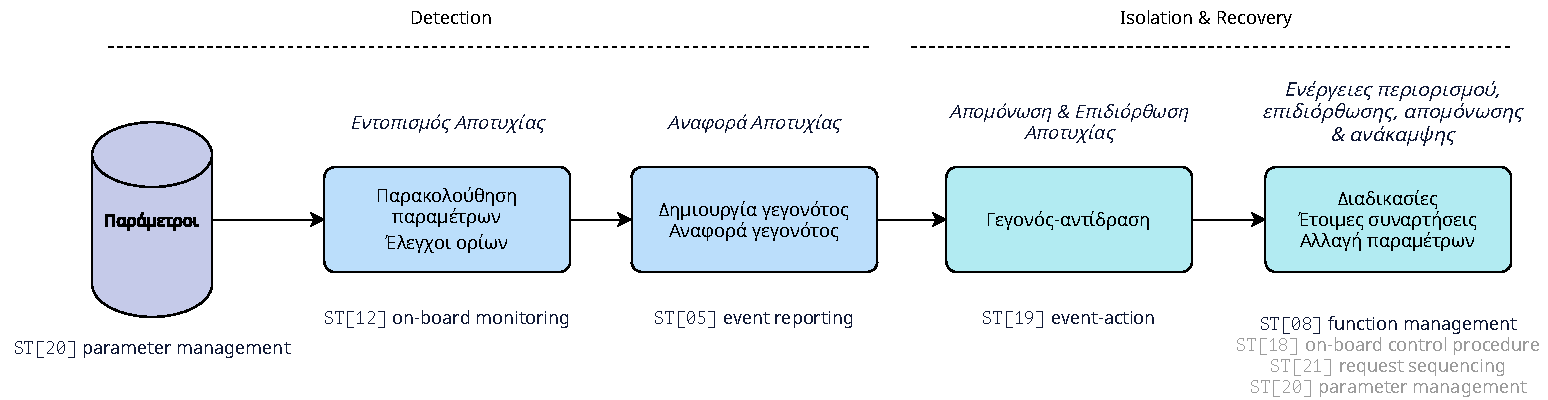
\includegraphics{FDIRpus}
	\caption{Η ροή δεδομένων για τον εντοπισμό της αποτυχίας}
	\label{fig:fdirpus}
\end{figure*}

Η παραπάνω λογική συνοψίζεται στο \Cref{fig:fdirpus}. Η σημασία της έγκειται στο ότι προσφέρει έναν \textbf{δομημένο} τρόπο το σύστημα να διαχειριστεί οποιοδήποτε πρόβλημα προβλεφθεί, αλλά ταυτόχρονα να δίνει τη δυνατότητα στους χειριστές \& κατασκευαστές:
\begin{compactitem}
	\item Να λάβουν όλες τις πληροφορίες για τη λειτουργική κατάσταση των εξαρτημάτων και τιμές των αισθητήρων
	\item Να παρέμβουν με ασφάλεια εξ' ολοκλήρου στη λειτουργία του \acs{FDIR} χωρίς μεταβολή του πηγαίου κώδικα
	\item Να απενεργοποιήσουν εν μέρει ή εντελώς το \acs{FDIR} αν χρειαστεί για διαγνωστικούς σκοπούς
	\item Να χρησιμοποιήσουν μία έτοιμη και δοκιμασμένη σουίτα λογισμικού των υπηρεσιών \acs{ECSS} για να υλοποιήσουν όλα τα παραπάνω, μειώνοντας το κόστος και τον χρόνο ανάπτυξης
	\item Να αποφευχθεί το ανεξέλεγκτο "hard-coding" διαδικασιών \acs{FDIR} σε διάφορα σημεία του κώδικα
\end{compactitem}


\chapter{\acs{FDIR} στο AcubeSAT}
\label{cap:acufdir}

Στο παρακάτω κεφάλαιο γίνεται ανάλυση περίπτωσης (case study) για την εφαρμογή των παραπάνω (\Cref{cap:savoir}) στην αποστολή του AcubeSAT (\Cref{cap:acubesat}). Πιο συγκεκριμένα, μελετώνται οι σχεδιαστικές αποφάσεις που λήφθηκαν, τα κομμάτια των προτύπων που εφαρμόστηκαν, και οι συγκεκριμένες ενέργειες που εξαρτώνται από την αποστολή \autocite{FMEA}.

\section{Βασικές αρχές του \acs{FDIR}}
\label{sec:fdirbaspri}

Οι απαιτήσεις του \acs{FDIR} του AcubeSAT προέρχονται κυρίως από τις δυνατότητες του σχεδιασμού του συστήματος (\Cref{cap:acubesat}) και του πειράματος (\Cref{sec:su_fdir}). Πιο συγκεκριμένα, οι βασικές αρχές είναι:

\begin{enumerate}
	\item \textbf{Αρθρωτή δομή} (modularity): Το \acs{FDIR} δεν θα πρέπει να είναι κλειδωμένο (hard-coded) στο λογισμικό, αλλά θα πρέπει να επιτρέπει τις εύκολες μεταβολές και να βασίζεται σε μία δομημένη βάση δεδομένων.
	\item \textbf{Αυτονομία}: Ο δορυφόρος θα πρέπει να μπορεί να επιβιώσει σε τροχιά για πάνω από \SI{24}{\hour} χωρίς επικοινωνία με το σταθμό βάσης, και να μπορεί να συντηρήσει οποιαδήποτε λειτουργία συστήματος, και ειδικότερα το επιστημονικό πείραμα.
	\item \textbf{Διαμορφωσιμότητα} σε τροχιά: Είναι πολύ δύσκολο να προβλεφθεί η ακριβής συμπεριφορά του δορυφόρου σε τροχιά. Ως εκ τούτου, θα πρέπει να δίνεται η δυνατότητα στους χειριστές για πλήρη διαμόρφωση και ρύθμιση του \acs{FDIR} αν χρειαστεί. Η διαμορφωσιμότητα αυτή μπορεί να περιλαμβάνει απενεργοποίηση ελέγχων, αλλαγές επικίνδυνων ορίων, ή ακόμα και εγκαστάσταση νέων ελέγχων.
	\item \textbf{Παρατηρησιμότητα}, προσφέροντας έναν μεγάλο όγκο πληροφορίας στο σταθμό βάσης για τη διάγνωση των προβλημάτων.
	\item \textbf{Καμία υπόθεση} για λειτουργικότητα εξοπλισμού. Κάθε κατάσταση σφάλματος στο λογισμικό και κάθε μη έγκυρη είσοδος λογισμικού θα πρέπει να θεωρείται πιθανή.
	\item \textbf{Διαθεσιμότητα}: Το AcubeSAT \g{επωφελείται από μεγαλύτερους χρόνους σε τροχιά, αφού αυτό επιτρέπει το κατέβασμα μεγαλύτερου όγκου δεδομένων και περισσότερα επιστημονικά αποτελέσματα.} Επιπλέον, σύντομη διακοπή κάποιου από τα υποπειράματα μπορεί εγγενώς να οδηγήσει σε πλήρη αποτυχία του. Ως εκ τούτου, το AcubeSAT ακολουθεί μία \emph{λειτουργική} (fail-operational) και όχι \emph{ακίνδυνη} (fail-safe) λογική, και προσπαθεί να διορθώσει βλάβες χωρίς να διακόψει τη ροή των λειτουργιών του.
	\item \textbf{Σχεδιασμός} βασισμένος στις αποτυχίες: Το AcubeSAT προσπαθεί να συμπεριλάβει πιθανές αποτυχίες στα βασικά κομμάτια του σχεδιασμού, αυξάνοντας την αξιοπιστία ακόμα και πριν την εφαρμογή του συστήματος \acs{FDIR}.
\end{enumerate}

Οι παραπάνω απαιτήσεις καλύπτονται από τη λογική του \acs{SAVOIR} που παρουσιάστηκε στο \Cref{cap:savoir}, η οποία υλοποιείται και στο AcubeSAT.

Τα επίπεδα του \acs{FDIR} στο AcubeSAT είναι τα εξής 3:
\begin{enumerate}[label=Επίπεδο \arabic*]
	\item \textbf{Μονάδα}/\textbf{Εξάρτημα}: Εδώ γίνεται εντοπισμός και διόρθωση των αποτυχιών σε επίπεδο ενός εξαρτήματος (π.χ. \g{αισθητήρα θερμοκρασίας}). Οι απλές αποτυχίες στο επίπεδο αυτό δεν επηρεάζουν το παραπάνω επίπεδο, και μπορούν να διορθωθούν τυπικά με απλές ενέργειες (π.χ. επανεκκίνηση εξαρτήματος).
	
	Το επίπεδο αυτό το αναλαμβάνει συνήθως ο μικροελεγκτής του κάθε υποσυστήματος. Παρ' όλο που οι αποτυχίες εδώ μπορεί να μη γίνουν αντιληπτές από τα υπόλοιπα υποσυστήματα, η αντίστοιχη τηλεμετρία πρέπει να παραχθεί ώστε για να υπάρχει η κατάλληλη παρατηρησιμότητα από το σταθμό βάσης, ή να προβλεφθούν άλλες βλάβες που δεν έγιναν αντιληπτές από το δορυφόρο.
	\item \textbf{Υποσύστημα}: Εδώ ανήκουν σοβαρές αποτυχίες που επηρεάζουν την πλήρη λειτουργία ενός υποσυστήματος (π.χ. υπερθέρμανση, καμία απάντηση από το υποσύστημα κλπ.). Οι αποτυχίες αυτές δεν οδηγούν το δορυφόρο απαραίτητα σε παύση, αλλά μπορούν να διορθωθούν με επανεκκινήσεις ή αλλαγές των ρυθμίσεων του υποσυστήματος.
	
	Οι αποτυχίες σε επίπεδο υποσυστήματος και πάνω αναλαμβάνονται από τον μικροελεγκτή του \acf{OBC}, που περιέχει το λογισμικό για τον εντοπισμό και επιδιόρθωσή τους. Σε περίπτωση όμως αποτυχίας του \acf{OBC}, το \acf{ADCS} αναλαμβάνει την ευθύνη του \acf{FDIR}.
	\item \textbf{Σύστημα}: Εδώ ανήκουν αποτυχίες οι οποίες δεν μπορούν να διορθωθούν αυτόνομα από το σύστημα (π.χ. ελλιπής ισχύς, υπερβολικά μεγάλη γωνιακή ταχύτητα). Ο τρόπος επιδιόρθωσης εδώ είναι συνήθως η είσοδος σε \emph{ασφαλή λειτουργία}, όπου πραγματοποιούνται μόνο οι πιο βασικές και ζωτικές διαδικασίες του δορυφόρου, μέχρι το σφάλμα να επιδιορθωθεί από τον σταθμό βάσης.
\end{enumerate}

\section{Μελέτη διαφορετικών αρχιτεκτονικών}

Προτού μελετήσουμε τη δομή του \acs{FDIR}, έχει νόημα να μελετήσουμε διαφορετικές αρχιτεκτονικές αποφάσεις που μπορούν να ληφθούν κατά το σχεδιασμό ενός μικρού δορυφορικού συστήματος. Πιο συγκεκριμένα, θα συγκρίνουμε τις δομές \autocite{birolini_reliability_engineering_2004}:

\begin{enumerate}
	\item \textbf{Απλού εξαρτήματος}
	\item \textbf{Διπλού πλεονασμού}, όπου έχουμε δύο όμοια εξαρτήματα που πραγματοποιούν την ίδια λειτουργία, και το ένα μπορεί να αντικαταστήσει το άλλο.Η συνδεσμολογία αυτή μπορεί να ακολουθεί με τη λογική του \textbf{ψυχρού πλεονασμού} ή του \textbf{ενεργού πλεονασμού}.
	
	Στον \textbf{ψυχρό πλεονασμό}, μόνο ένα από τα εξαρτήματα λειτουργεί κάθε φορά, και ένα εξωτερικό κύκλωμα\footnote{Ή τα ίδια τα εξαρτήματα, στην περίπτωση του θερμού πλεονασμού \autocite[20]{SAVOIR-HB-003}} ελέγχει ποιό από τα δύο δεν βρίσκεται σε κατάσταση σφάλματος, για να του παραδώσει τον έλεγχο.
	
	Στον \textbf{ενεργό πλεονασμό}, και τα δύο εξαρτήματα είναι λειτουργικά ταυτόχρονα, πραγματοποιώντας τις ίδιες διαδικασίες, και το ένα εξάρτημα μπορεί να αναλάβει τις λειτουργικές ευθύνες σε περίπτωση βλάβης του άλλου.
	
	\item \textbf{Τριπλού πλεονασμού με ψηφοφορία} (triple modular redundancy), όπου έχουμε τρία εξαρτήματα που πραγματοποιούν συνεχώς τους ίδιους υπολογισμούς, και ένα κύκλωμα ψηφοφορίας επιλέγει την έξοδο που έχει την πλειοψηφία από τα 3 εξαρτήματα.
\end{enumerate}

\begin{figure}[h]
	\centering
	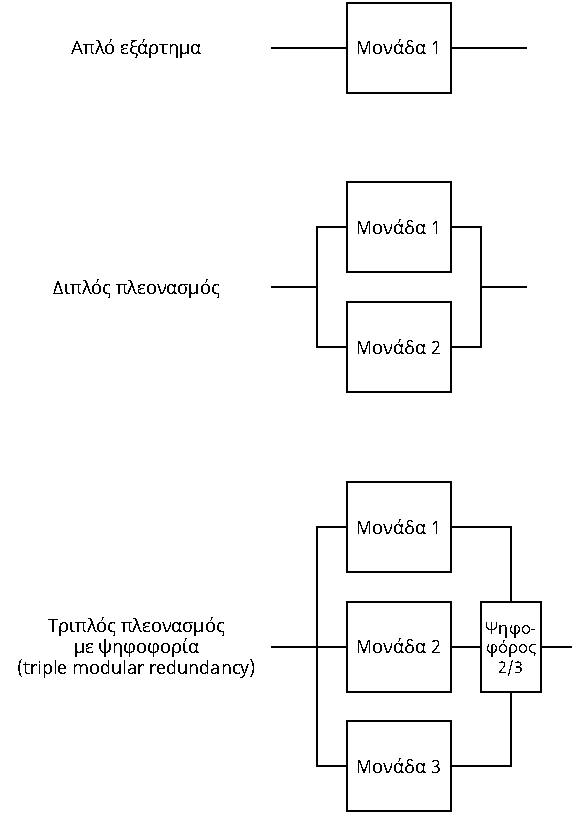
\includegraphics[width=.6\textwidth]{RedunSchemes-el}
	\caption{Οπτική απεικόνιση των διαφορετικών μορφών σύνδεσης που θα εξεταστούν}
\end{figure}

Η σύγκριση των συστημάτων αυτών θα γίνει σε επίπεδο μόνιμων και προσωρινών βλαβών:

\begin{itemize}
	\item \g{Στις \textbf{μόνιμες βλάβες} εξετάζουμε συμβάντα (π.χ. ακτινοβολία, απώλεια μνήμης) τα οποία δεν μπορούν να διορθωθούν και οδηγούν σε απώλεια της αποστολής. Η μελέτη εδώ γίνεται με βάση την έννοια της αξιοπιστίας (\e{reliability}) \( R \), δηλαδή της πιθανότητας το σύστημα να επιζήσει εντός μιας χρονικής περιόδου \( t \).}
	\item Στις \textbf{προσωρινές βλάβες} εξετάζουμε συμβάντα (π.χ. αλλαγές bit, bugs λογισμικού, λάθη στη μεταφορά μηνυμάτων) που είναι παροδικά και επηρεάζουν συνήθως μόνο μία μέτρηση, μία ενέργεια ή ένα αποτέλεσμα. Εδώ η μελέτη γίνεται με βάση την έννοια του ρυθμού βλαβών (failure rate) \( \lambda \), δηλαδή της συχνότητας των αποτυχιών.
\end{itemize}

\selectlanguage{greek}

Στην παρούσα ανάλυση δεν είναι εύκολο να χρησιμοποιηθούν ακριβείς τιμές αξιοπιστίας και ρυθμού αποτυχιών για τα εξαρτήματα, καθώς δεν υπάρχουν στη βιβλιογραφία διαθέσιμα στοιχεία μεγάλης κλίμακας για τις αποτυχίες εξαρτημάτων στο διάστημα \e{\autocite{esatec-qqd_effective_reliability_2016}}. Επομένως, η ανάλυση θα γίνει σε ένα εύρος τιμών αξιοπιστίας και ρυθμού σφαλμάτων.

Ενδεικτικά, αναφέρουμε ότι η τάξη μεγέθους του ρυθμού αποτυχιών μιας συσκευής λόγω ακτινοβολίας μπορεί να εκτείνεται μεταξύ \SIrange{1e-8}{1e3}{} \(\frac{\text{αποτυχίες}}{\text{ημέρα}}\), εξαρτώμενη από το περιβάλλον ακτινοβολίας, τη σοβαρότητα της βλάβης, και την κατασκευή της κάθε συσκευής \e{\autocite[158-159]{gupta_analysis_single_2017}}.

Ο κώδικας που χρησιμοποιήθηκε για όλα τα παρακάτω παραδείγματα βρίσκεται στο \Cref{app:analysisjl}.

\subsection{Μόνιμες βλάβες (ανάλυση αξιοπιστίας)}

\paragraph{Ιδεατός ψηφοφόρος}

Αν θεωρήσουμε ότι η αξιοπιστία ενός εξαρτήματος είναι \(R\), η αξιοπιστία \emph{δύο εξαρτημάτων} συνδεδεμένων παράλληλα είναι \e{\autocite[31]{birolini_reliability_engineering_2004}}:
\begin{equation}
R_2 = 2R - R^2 = 1 - (1 - R)^2 \label{eq:dual_redun}
\end{equation}

\marginnote{Σε όλες τις αναλύσεις υποθέτουμε ότι τα ευάλωτα εξαρτήματα είναι πανομοιότυπα και έχουν τα ίδια χαρακτηριστικά αξιοπιστίας.}
Η \eqref{eq:dual_redun} ισχύει τόσο στον ψυχρό, όσο και στον ενεργό πλεονασμό, καθώς θεωρούμε ότι το σύστημα μπορεί να ανακάμψει από μόνιμες βλάβες και στις δύο περιπτώσεις, μετακινώντας τη "δικαιοδοσία" ελέγχου στο ανεπηρέαστο εξάρτημα.

Η αξιοπιστία του συστήματος \emph{τριπλής ψηφορορίας} είναι \e{\parencite[31]{birolini_reliability_engineering_2004}}:
\begin{align}
R_3 &= \sum_{i=k}^{n} \binom{n}{i} R^i (1-R)^{n-i}\nonumber\\
&= \sum_{i=2}^{3} \binom{3}{i} R^i (1-R)^{3-i} \nonumber\\
&= \binom{3}{2} R^2 (1-R) + \binom{3}{3} R^3 (1-R)^0 \nonumber\\
&= 3R^2 - 3R^3 + R^3 = 3R^2 - 2R^3
\label{eq:tmr}
\end{align}

Εδώ αξίζει να σημειωθεί πως το σύστημα τριπλής ψηφοφορίας θεωρεί έναν απλό ψηφοφόρο, και σε περίπτωση \emph{μόνιμης βλάβης και των δύο ευάλωτων εξαρτημάτων}, το σύστημα θεωρείται πως δεν μπορεί να ανακάμψει.

\begin{figure}
	\centering
	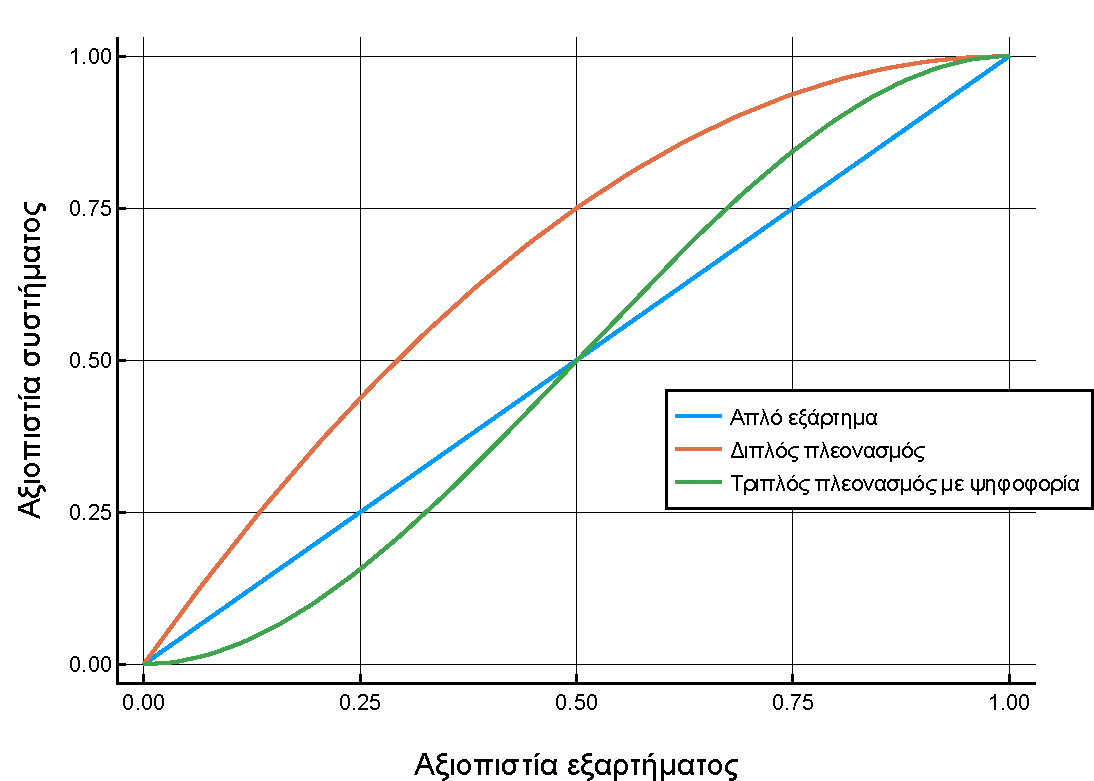
\includegraphics{analysis/reliability_norepair}
	\caption{Ανθεκτικότητα σύνθετου συστήματος σε μόνιμες βλάβες (θεωρώντας αλάνθαστο ψηφοφόρο)}
	\label{fig:reliability_norepair}
\end{figure}

Τα αποτελέσματα εφαρμογής των \eqref{eq:dual_redun} και \eqref{eq:tmr} φαίνονται στο \Cref{fig:reliability_norepair}. Μπορεί να διακριθεί πως η χρήση δύο πλεονάζοντων εξαρτημάτων αυξάνει σε έναν βαθμό την αξιοπιστία του συστήματος, σε σχέση με το απλό εξάρτημα, καθώς οι βλάβες του ενός εξαρτήματος μπορούν να διορθωθούν, αλλά οι βλάβες και στα δύο είναι καταστροφικές. Αντίθετα, \textbf{ο τριπλός πλεονασμός εισάγει περισσότερα σημεία αποτυχίας}. Καθώς η αποτυχία οποιουδήποτε συνδυασμού 2 εκ των 3 εξαρτημάτων είναι καταστροφική, ο τριπλός πλεονασμός υστερεί στις μόνιμες βλάβες σε σχέση με τον διπλό.

\paragraph{Ευάλωτος ψηφοφόρος}

Ιδιαίτερο ενδιαφέρον έχει η μελέτη της περίπτωσης του ευάλωτου κυκλώματος ψηφοφορίας, το οποίο συνδέεται 

\subsection{Προσωρινές βλάβες (ανάλυση ρυθμού βλαβών)}

\selectlanguage{english}


\begin{figure}
	\centering
	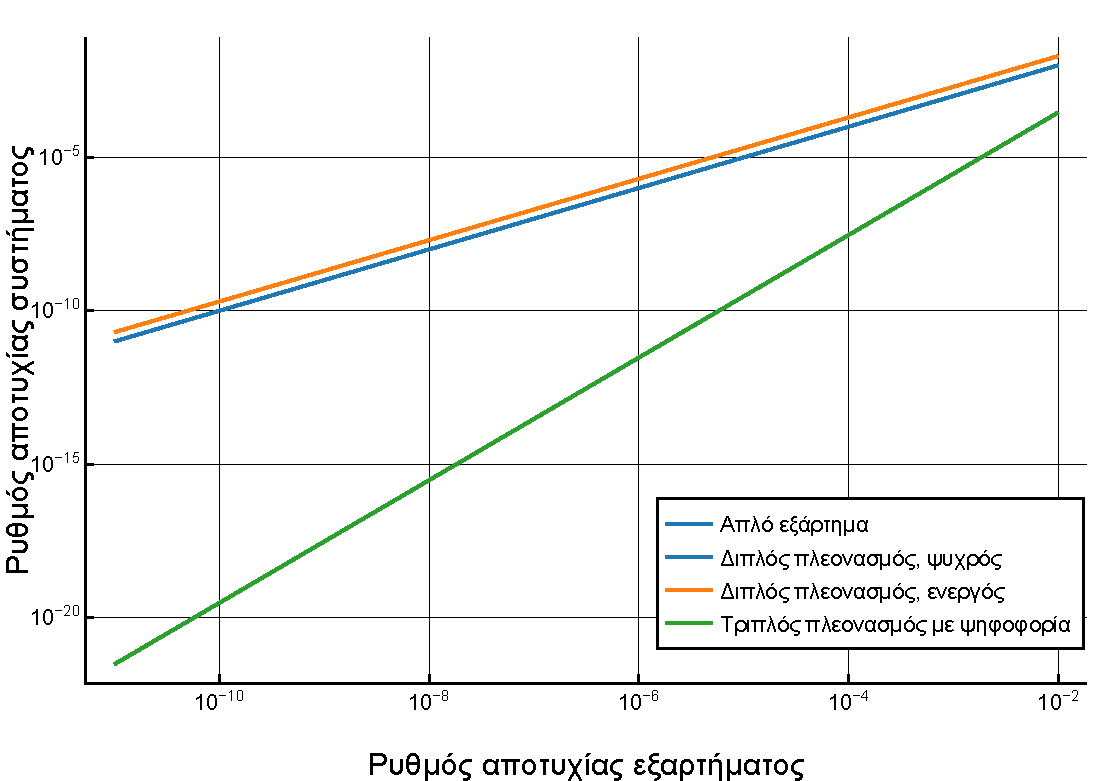
\includegraphics{analysis/reliability_repair}
	\caption{\g{Ανθεκτικότητα σύνθετου συστήματος σε παροδικά σφάλματα (θεωρώντας αλάνθαστο ψηφοφόρο)}}
	\label{fig:reliability_repair}
\end{figure}

\draft{επεξήγηση \& συμπεράσματα}

\FloatBarrier
\section{Λεπτομερείς Ενέργειες του FDIR}

Στην παρακάτω ενότητα παρουσιάζεται η λίστα με τους πιθανούς τρόπους εντοπισμού, πρόληψης και αντιμετώπισης των σφαλμάτων που εμφανίζονται στον δορυφόρο. Για την κάθε πιθανή αποτυχία που εντοπίζεται στο \acs{FMEA} \autocite{retselis_acubesat_fmea_2020}, επιλέγεται ένας ή περισσότεροι τρόποι εντοπισμού και διόρθωσης από αυτούς τους πίνακες, και προσαρμόζονται στο εκάστοτε στοιχείο.

\clearpage
\subsection{Τρόποι εντοπισμού αποτυχιών}
\begin{table*}[h]
	\centering
	\caption[][10pt]{Τρόποι εντοπισμού αποτυχιών \acs{FDIR} του AcubeSAT}
	\label{tab:fdir_detect}
	\renewcommand{\arraystretch}{1.3}
	\begin{tabularx}{\textwidth}{@{}cL{5cm}X@{}}
		\toprule
		Επίπεδο & Μέθοδος & Περιγραφή \\ \midrule
		Μονάδα & \textbf{Αυτο-δοκιμή δεν επιστρέφει σωστή τιμή} & Τα συνδεδεμένα περιφερειακά μπορεί να διαθέτουν δυνατότητες αυτο-δοκιμής (self-test) ή να έχουν αποθηκευμένες προκαθορισμένες τιμές που δεν μπορούν να μεταβληθούν. \\
		Μονάδα & \textbf{Τιμή εκτός ορίων} & Μη αναμενόμενες τιμές των αισθητήρων μπορεί να σημαίνουν επικίνδυνες περιβαλλοντικές συνθήκες, ή απλά ελαττωματικούς (π.χ. \acs{SEFI}) αισθητήρες. Ο διπλός ή τριπλός πλεονασμός μπορεί να αυξήσει την παρατηρησιμότητα σε αυτή την περίπτωσ \\
		Μονάδα & \textbf{Τιμές κοντινών αισθητήρων πολύ διαφορετικές} &  \\
		Μονάδα & \textbf{Καμία απάντηση ή ασυνάρτητες τιμές} & Η μονάδα ή η διεπαφή μπορεί να είναι ελαττωματική \\
		Μονάδα & \textbf{Υπερβολικά μεγάλη κατανάλωση ρεύματος} & Μπορεί να παρατηρηθεί σε μονάδες που πάσχουν από βραχυκυκλώματα ή \acs{SEL} \\
		Μονάδα & \textbf{Λάθος σε αλγόριθμο εντοπισμού \& διόρθωσης σφαλμάτων} &  \\
		Υποσύστημα & \textbf{Καμία απάντηση σε εντολές \acs{CAN}} & Μπορεί να οφείλεται σε αποτυχία του υποσυστήματος, ή του πομποδέκτη \acs{CAN} \\
		Σύστημα & \textbf{Καμία τηλεεντολή δεν έχει ληφθεί για κάποιο χρονικό διάστημα} & Ο \acs{GS} στέλνει περιοδικές εντολές "ανανέωσης" στον δορυφόρο σε κάθε πέρασμα. Η μη λήψη σημαίνει απώλεια επικοινωνίας. \\
		Λογισμικό & \textbf{Εξαίρεση υλικού} & Μπορεί να οφείλεται σε διαίρεση με το 0, προσπάθεια πρόσβασης σε μη προσβάσιμη μνήμη κλπ. \\
		Λογισμικό & \textbf{Αποτυχημένος έλεγχος ορισμάτων} &  \\
		Λογισμικό & \textbf{Μη αναμενόμενη επανεκκίνηση μικροελεγκτή} &  \\
		Λογισμικό & \textbf{Διαφορά στις τιμές μεταβλητών με πλεονασμό} &  \\ \bottomrule
	\end{tabularx}
\end{table*}

\clearpage
\subsection{Προληπτικές δράσεις}

\begin{table*}[h]
	\centering
	\caption[][10pt]{Προληπτικές δράσεις \acs{FDIR} του AcubeSAT}
	\label{tab:fdir_preventive}
	\renewcommand{\arraystretch}{1.5}
	\begin{tabularx}{\textwidth}{@{}lcX@{}}
		\toprule
		\# & Επίπεδο & Δράση \\ \midrule
		1 & Υλικό & Μικροελεγκτής ανθεκτικός στην ακτινοβολία \\
		2 & Υλικό & Κυκλώματα παρακολούθησης μικροελεγκτή (watchdogs) \\
		3 & Υλικό & Κυκλώματα παρακολούθησης συστήματος (watchdogs) \\
		4 & Υλικό & Αλγόριθμοι εντοπισμού \& διόρθωσης σφαλμάτων \\
		5 & Υλικό & Διπλός πλεονασμός στη μνήμη λογισμικού \\
		6 & Υλικό & Κυκλώματα περιορισμού ρεύματος \\
		7 & Υλικό & Προστασία υπέρτασης και υπερέντασης υποσυστημάτων \\
		8 & Υλικό & Χρήση προσωρινής μνήμης \acs{MRAM} ανθεκτικής στην ακτινοβολία \\
		9 & Υλικό & Διπλός πλεονασμός στους αισθητήρες \\
		10 & Υλικό & Υποβιβασμός προδιαγραφών σε ηλεκτρονικά ισχύος \\
		11 & Υλικό & Τοποθέτηση ευάλωτων εξαρτημάτων στο κέντρο, ώστε να μειωθεί η επίδραση της ακτινοβολίας \\
		12 & Υλικό & Επιλογή εξαρτημάτων με αποτελέσματα δοκιμών ακτινοβολίας \\
		13 & Υλικό & Διπλός πλεονασμός στον δίαυλο \acs{CAN} \\
		14 & Υλικό & Bit ισοτιμίας στον δίαυλο \acs{CAN} \\
		15 & Λογισμικό & Αλγόριθμοι εντοπισμού \& διόρθωσης σφαλμάτων \\
		16 & Λογισμικό & Σύστημα αρχείων ανθεκτικό σε βλάβες και απώλεια ισχύος \\
		17 & Λογισμικό & Φιλτράρισμα εισόδων \acs{ADCS} \\
		18 & Διαχειριστικά & Αυτόματες περιοδικές επανεκκινήσεις \\
		19 & Διαχειριστικά & Αποφυγή επικίνδυνων διεργασιών σε περιοχές με υψηλό υπόβαθρο ακτινοβολίας \\
		20 & Διαχειριστικά & Αξιολόγηση των διαθέσιμων πόρων \& προϋπολογισμών πριν από την έναρξη υποπειράματος \\ \bottomrule
	\end{tabularx}
\end{table*}

\clearpage
\subsection{Διορθωτικές δράσεις}

\begin{table*}[h]
	\centering
	\caption[][10pt]{Διορθωτικές δράσεις \acs{FDIR} του AcubeSAT}
	\label{tab:fdir_corrective}
	\renewcommand{\arraystretch}{1.5}
	\begin{tabularx}{\textwidth}{@{}lL{3cm}X@{}}
		\toprule
		Επίπεδο & Δράση & Περιγραφή \\ \midrule
		& \textbf{Καμία} & Πολλές φορές υπάρχουν προβλήματα τα οποία διορθώνονται αυτόνομα, ή δεν υπάρχει τρόπος διόρθωσής τους (και δεν επηρεάζουν σημαντικά τη λειτουργία του υπόλοιπου δορυφόρου). \\
		Μονάδα & \textbf{Επανεκκίνηση μονάδας} & Αυτή η μέθοδος ανάκαμψης συνδέεται με προσωρινά προβλήματα που μπορεί να εμφανιστούν στο λογισμικό ή το υλικό μιας συσκευής. Τέτοιες βλάβες μπορεί να προέρχονται από λάθη σχεδιασμού (bugs) που δεν δοκιμάστηκαν εκτενώς, ή από αλλαγές κατάστασης των τρανζίστορ που οφείλονται σε ακτινοβολία. \\
		Μονάδα & \textbf{Διακοπή και ανάκτηση ρεύματος} & Μερικά προβλήματα μπορεί να μην διορθώνονται παρά μόνον αν διακοπεί η παροχή ρεύματος στην πληγείσα μονάδα. Φαινόμενα όπως SEL μπορούν να απαιτούν τέτοιες δράσεις. \\
		Μονάδα & \textbf{Απομόνωση μονάδας} & Αν μία μονάδα δεν μπορεί να επιδιορθωθεί, το επόμενο βήμα είναι να αγνοηθούν οι τιμές της ή να αποσυνδεθεί από το ρεύμα, ώστε να μην επηρεαστεί το υπόλοιπο σύστημα από τις λανθασμένες ενέργειές της. \\
		Υποσύστημα & \textbf{Επανεκκίνηση υποσυστήματος} & Φαινόμενα ακτινοβολίας ή άλλες αποτυχίες μπορεί να οδηγήσουν ένα υποσύστημα σε μη αναμενόμενη κατάσταση, από την οποία να μπορεί να ξεφύγει μόνο με επανεκκίνηση. \\
		Υποσύστημα & \textbf{Αναδιαμόρφωση υποσυστήματος} & Αν υπάρχει μια μόνιμη βλάβη που δεν μπορεί να διορθωθεί με επανεκκίνηση, ο δορυφόρος πρέπει να προσπαθήσει να συνεχίσει την κανονική λειτουργία. Αυτό μπορεί να γίνει αλλάζοντας τις προεπιλεγμένες ρυθμίσεις ενός υποσυστήματος, π.χ. μέσω επιλογής διαφορετικών αισθητήρων, μέσω αλλαγής της λειτουργίας του υποσυστήματος, ή μέσω ανάθεσης των καθηκόντων του σε μια άλλη λειτουργική μονάδα. \\
		Σύστημα & \textbf{Διακοπή τρέχουσας λειτουργίας} & Μπορεί να διακοπεί η εκτελούμενη διαδικασία (π.χ. έναρξη ενός πειράματος, αποστολή TM), εφ' όσον δεν επηρεάζει την ασφάλεια του συστήματος. \\
		Σύστημα & \textbf{Είσοδος σε ασφαλή λειτουργία (safe mode)} & Αυτό είναι το τελευταίο βήμα στις διορθωτικές προσπάθειες. Ο δορυφόρος εισέρχεται στην ασφαλή λειτουργία ώστε να αποτρέψει περαιτέρω διάδοση της βλάβης. \\ \bottomrule
	\end{tabularx}
\end{table*}

\FloatBarrier
\section{Λειτουργική ροή του \acs{FDIR}}
\label{sec:fdir_operating_modes}

Σε αυτήν την ενότητα παρουσιάζονται οι ροές και διαδικασίες του \acs{FDIR} που εκτελούνται σε τροχιά. Αν και η διαδικασία για την κάθε δομική μονάδα και την κάθε διαδικασία είναι διαφορετική, ακολουθείται ένας γενικότερος ιεραρχικός κανόνας που ξεκινάει από τη χαμηλότερη βαθμίδα (μονάδας/εξαρτήματος), και προχωρά στο επίπεδο συστήματος, αν η εξεταζόμενη βλάβη συνεχίζει να το επηρεάζει.

Μετά από την επιδιόρθωση (ή προσπάθεια επιδιόρθωσης) της βλάβης, η ευθύνη μεταφέρεται πλέον στους χειριστές, που πρέπει να εντοπίσουν την βασική πηγή του προβλήματος, και να πραγματοποιήσουν τις απαραίτητες ενέργειες, αν χρειάζεται, για τη μόνιμη επιδιόρθωσή του.

\begin{figure*}[h]
	\includegraphics{FDIRgeneric-el}
	\caption{Γενική ροή του \acs{FDIR} σε λειτουργικές καταστάσεις του δορυφόρου}
	\label{fig:generalflow}
\end{figure*}

Η γενική ροή που παρουσιάζεται στο \Cref{fig:generalflow} περιγράφει την τυπική διαδικασία επίλυσης μιας αποτυχίας στο δορυφόρο. Η διαδικασία που ακολουθείται είναι ιεραρχική, ξεκινάει από το χαμηλό επίπεδο, και μπορεί να καταλήξει μέχρι και το επίπεδο συστήματος. Πιο συγκεκριμένα:
\begin{enumerate}
	\item Αν μια παρατηρούμενη παράμετρος είναι εκτός ορίων, πρώτα επιχειρείται επιδιόρθωση σε επίπεδο μονάδας με \textbf{απλές ενέργειες} (π.χ. reset, επανεκκίνηση).
	\item Αν η αποτυχία συνεχίσει να υφίσταται, τότε γίνεται προσπάθεια επίλυσής της σε επίπεδο υποσυστήματος. Για κρίσιμα εξαρτήματα, αυτό μπορεί να σημαίνει επανεκκίνηση ολόκληρου του υποσυστήματος· διαφορετικά, μπορεί να γίνει απλή απενεργοποίηση της μονάδας.
	
	\marginnote{Μία εναλλακτική μέθοδος υλοποίησης είναι να οριστεί μια παράμετρος που δείχνει την κατάσταση ή το τρέχον βήμα του \acs{FDIR} για την κάθε μονάδα, και οι ορισμοί παρακολούθησης να πυροδοτούνται ανάλογα με την τιμή αυτής της παραμέτρου.}
	Τεχνικά, ο διαχωρισμός μεταξύ των επιπέδων μονάδας και υποσυστήματος επιτυγχάνεται με κατάλληλη αξιοποίηση του \textbf{\texttt{ST[12]} on-board monitoring service} (\Cref{sec:pus}). Με την παράμετρο \textbf{repetition number} (αριθμός επαναλήψεων), ο χειριστής μπορεί να ορίσει το κατώφλι στη διάρκεια ύπαρξης της αποτυχίας που σηματοδοτεί απλή επιδιόρθωση ή βαρύτερα μέτρα. Για παράδειγμα, \( 2 \) μετρήσεις εκτός ορίων οδηγούν σε επανεκκίνηση του αισθητήρα, ενώ \( 5 \) μετρήσεις εκτός ορίων μπορεί να οδηγήσουν σε πλήρη απομόνωση/απενεργοποίησή του.
	\item Αν η αποτυχία συνεχίσει να υφίσταται αλλά δεν είναι κρίσιμη, απενεργοποιείται η μονάδα μόνιμα, καθώς και οι έλεγχοι του \acs{FDIR} για αυτήν, και αναδιαμορφώνεται αν χρειάζεται το υποσύστημα.
	
	Σε αυτό το σημείο πρέπει να τονιστεί πως η απενεργοποιημένη μονάδα δεν μπορεί να συνεισφέρει σε οποιαδήποτε λειτουργία του δορυφόρου. Η υπηρεσία \texttt{ST[12]} επιτρέπει τη χρήση των \textbf{check validity conditions} (συνθηκών εγκυρότητας ελέγχου), που μπορούν να απενεργοποιήσουν έναν έλεγχο αν αυτός αναφέρεται σε απενεργοποιημένη συσκευή ή άλλες συνθήκες που τον αποτρέπουν.
	\item Αν η αποτυχία συνεχίσει να υφίσταται, είναι κρίσιμη και δεν υπάρχει άλλος τρόπος διόρθωσής της, το σύστημα εισέρχεται σε \textbf{Ασφαλή Λειτουργία}.
\end{enumerate}

Όλα τα παραπάνω εκτελούνται στο υπόβαθρο του κάθε μικροελεγκτή σαν μία διεργασία του \acs{RTOS}, και, βασισμένα στις υπηρεσίες \acs{PUS}, είναι πλήρως προσαρμόσιμα από τον σταθμό βάσης.

\begin{table*}[h]
	\centering
	\caption{Σύνοψη της λειτουργικότητας του AcubeSAT σε διαφορετικές Λειτουργίες Συστήματος}
	\label{tab:acubesatmodes}
	\begin{tabular}{@{}llllll@{}}
		\toprule
		Υποσύστημα    & Εκτόξευση & Εκκίνηση & Κανονική                 & Επιστημονική        & Ασφαλής             \\ \midrule
		\acs{ADCS}  & \color{off} Off    & Σταθεροποίηση     & \color{on} Στόχευση                & Σταθεροποίηση     & Σταθεροποίηση       \\
		\acs{COMMS} & \color{off} Off    & \acs{UHF} μόνο & \color{on} \acs{UHF} και S-Band    & \acs{UHF} μόνο & \acs{UHF} μόνο   \\
		\acs{EPS}   & \color{off} Off    & \color{on} On             & \color{on} On                      & \color{on} On             & \color{on} On               \\
		\acs{OBC}   & \color{off} Off    & \color{on} On             & \color{on} On                      & \color{on} On             & \color{on} On               \\
		\acs{SU}    & \color{off} Off    & \color{off} Off            & Συντήρηση \& δεδομένα & \color{on} On             & Συντήρηση \\ \bottomrule
	\end{tabular}
	\vspace{1em}
\end{table*}

\subsection{Ασφαλής Λειτουργία}
\label{itm:safe_mode}

\begin{figure*}[h]
	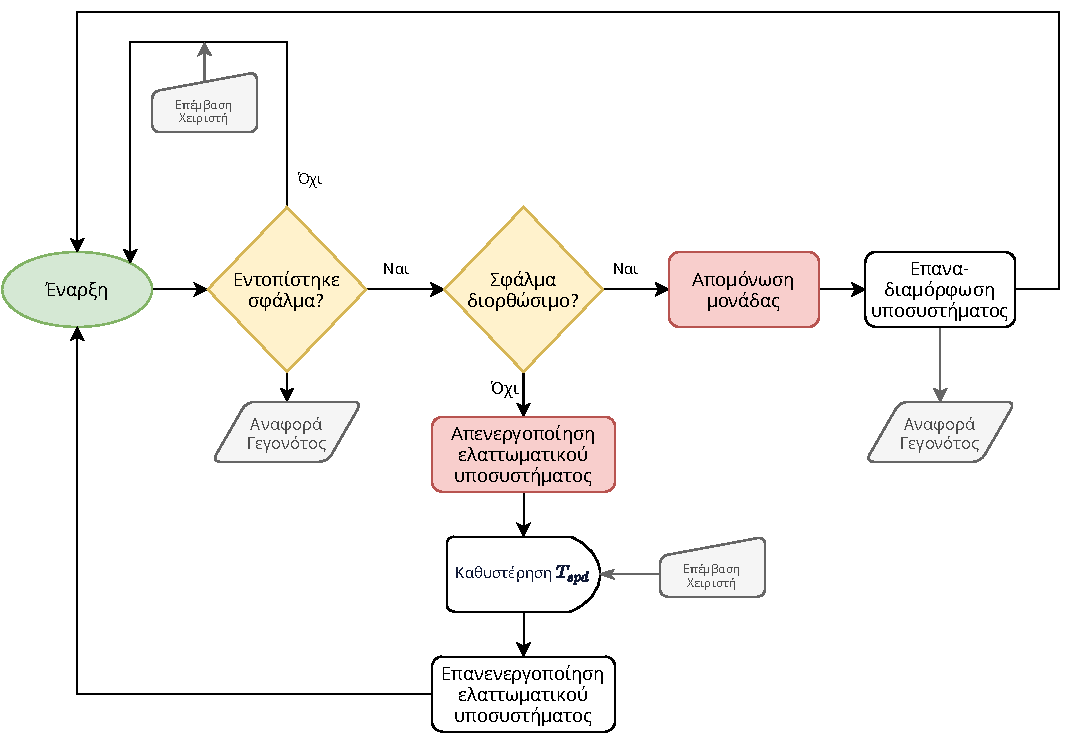
\includegraphics{FDIRsafe-el}
	\caption{Ροή του \acs{FDIR} στην Ασφαλή Λειτουργία}
	\label{fig:safeflow}
\end{figure*}

Ο στόχος της ασφαλούς λειτουργίας είναι να παρέχει μια ισχυρή, καλά δοκιμασμένη και ντετερμινιστική κατάσταση, όπου ο δορυφόρος μπορεί να λειτουργήσει αυτόνομα, μέχρι οι χειριστές μπορέσουν να αποκαταστήσουν την απειλητική για την αποστολή βλάβη. Το \acs{FDIR} της Ασφαλούς Λειτουργίας ακολουθεί επίσης το πρότυπο \acs{PUS} και τις προδιαγραφές του AcubeSAT (\Cref{sec:fdirbaspri}), συνεχίζοντας να επιτρέπει τις αλλαγές από τους χειριστές.
%Σε αυτή τη λογική, το \acs{FDIR} κατά τη διάρκεια της Ασφαλούς Λειτουργίας έχει σχεδιαστεί με βάση σκληρά κωδικοποιημένους ελέγχους και διαδικασίες ανάκτησης, για τον μικρό αριθμό ενεργών στοιχείων και λειτουργιών. Προβλέπεται επίσης να υλοποιηθεί η δυνατότητα απενεργοποίησης αυτών των ελέγχων μέσω εντολών εδάφους.

Στο AcubeSAT, η λειτουργικότητα του δορυφόρου είναι σημαντικά μειωμένη: το προφίλ στόχευσης προσπαθεί να πετύχει μόνο σταθεροποίηση, δεν εκτελούνται περίπλοκες λειτουργίες, και τα υποσυστήματα πραγματοποιούν μόνο συντήρηση. Ωστόσο, η επικοινωνία \ac{UHF} και η μετάδοση του περιοδικού ραδιοφάρου (beacon) εξακολουθούν να είναι ενεργές για λόγους παρατηρησιμότητας, και για να επιτραπεί η διόρθωση του εντοπισμένου προβλήματος.

\newthought{Η γενικη αρχιτεκτονικη} του \acs{FDIR} για την ασφαλή λειτουργία παρουσιάζεται στο \Cref{fig:safeflow}. Οι ενέργειες αποκατάστασης περιλαμβάνουν:
\begin{itemize}
	\item Απενεργοποίηση ολόκληρων \textbf{προβληματικών} υποσυστημάτων. Στην περίπτωση των \acs{ADCS} και \acs{OBC}, η ενέργεια αυτή συνοδεύεται από σημαντικά μειωμένη λειτουργικότητα, αλλά δεν επηρεάζει τη δυνατότητα ελέγχου του δορυφόρου. Από την άλλη πλευρά, η απενεργοποίηση των υποσυστημάτων \acs{COMMS} και \acs{EPS} εμποδίζει οποιαδήποτε επικοινωνία του σταθμού βάσης με το CubeSat. Η μόνη δράση που μπορεί να γίνει είναι η προσπάθεια επανεκκίνησης των υποσυστημάτων μετά από μία προκαθορισμένη χρονική καθυστέρηση, μέχρι ο δορυφόρος να βρεθεί για παράδειγμα σε πιο ευνοϊκές περιβαλλοντικές συνθήκες.
	\item Απομόνωση εξαρτημάτων και ανάλογη αναδιαμόρφωση των υποσυστημάτων. Ο μικρότερος αριθμός ενεργών εξαρτημάτων σε Ασφαλή Λειτουργία σημαίνει μια πιο ασφαλή διαδικασία σχεδιασμού και δοκιμών.
\end{itemize}


Οι χειριστές του AcubeSAT είναι υπεύθυνοι για τον προσδιορισμό της αιτίας της βλάβης και των διορθωτικών ενεργειών αμέσως μόλις λάβουν την τηλεμετρία που ανακοινώνει το σφάλμα, και πρέπει να επέμβουν άμεσα αφού αποφασιστεί μια ασφαλής πορεία δράσης. Η έξοδος από την ασφαλή λειτουργία μπορεί να γίνει \emph{μόνο μετά από εντολή του χειριστή}, και μόνο αφού διορθωθεί το αρχικό σφάλμα και δεν είναι ορατά άλλα σφάλματα (λόγω π.χ. διάδοσης της βλάβης). Οι δράσεις που μπορούν να λάβουν οι χειριστές είναι:
\begin{compactitem}
	\item Αλλαγή των ρυθμίσεων του δορυφόρου μέσω των υπηρεσιών \acs{ECSS}
	\item Πιο συχνά, αλλαγή του \textbf{λογισμικού} του δορυφόρου, ανεβάζοντας ανανεωμένες εικόνες δυαδικής μορφής\footnote{Η διαδικασία αυτή απαιτεί την εκτέλεση πλήρους καμπάνιας δοκιμών λογισμικού στη γη, και μία αξιόπιστη διαδικασία επαναπρογραμματισμού του δορυφόρου σε τροχιά \autocite[45]{DDJF_OBSW}}
	\item Μόνιμη απενεργοποίηση ελαττωματικών μονάδων
	\item Αναμονή μέχρι ο δορυφόρος να βρεθεί σε ευνοϊκή κατάσταση
	\item Καμία, αν η βλάβη εντοπίστηκε από λάθος, ή διορθώθηκε αυτόματα
\end{compactitem}

\section{Επόμενα βήματα}
Ο συνδυασμός \acs{FMEA} και \acs{HSIA} του AcubeSAT περιέχει 928 πιθανές αποτυχίες, εκ των οποίων οι 185 θεωρούνται υψηλής κρισιμότητας \autocite{retselis_acubesat_fmea_2020}.

Μετά από τη διατύπωση της αρχιτεκτονικής και του σχεδιασμού του \acs{FDIR}, έπεται η υλοποίησή του. Για αυτόν τον σκοπό, η ομάδα έχει αναπτύξει μία βιβλιοθήκη που υλοποιεί τις υπηρεσίες \acs{PUS}\footurl{https://gitlab.com/acubesat/obc/ecss-services} και μπορεί να καλύψει τις ανάγκες της παρούσας ενότητας.

Η επαλήθευση του \acs{FDIR} είναι το τελευταίο κομμάτι της διαδικασίας, και περιλαμβάνει έλεγχο της κάθε επίφοβης αποτυχίας, μέσω προσομοίωσης με υλικό ή λογισμικό.

\chapter{\g{Πρακτική επίδειξη του} \acs{FDIR}}
\label{cap:practical}

Ως πείραμα "proof-of-concept" για την υλοποίηση του \ac{FDIR} του AcubeSAT, προετοιμάσαμε μια πρακτική διάταξη για την προσομοίωση της συμπεριφοράς του δορυφόρου (\Cref{fig:block}). Η διάταξη αποτελείται από:
\begin{compactitem}
	\item Έναν Cortex-M7 \textbf{μικροελεγκτή}, που χρησιμοποιείται για την προσομοίωση ενός \textbf{υποσυστήματος δορυφόρου}
	\item Έναν αριθμός πλεονάζοντων \textbf{αισθητήρων} θερμοκρασίας, που προσομοιώνουν πιθανά σημεία \textbf{αστοχίας}.
	\item Το συνοδευτικό \textbf{λογισμικό} που περιλαμβάνει την υλοποίηση των υπηρεσιών \ac{ECSS} και της λογικής \ac{SAVOIR} \ac{FDIR}.
	\item Έναν υπολογιστή, που χρησιμεύει ως \textbf{σταθμός βάσης} για την παροχή των απαραίτητων δυνατοτήτων ελέγχου και παρατήρησης.
\end{compactitem}

\begin{figure*}[h]
	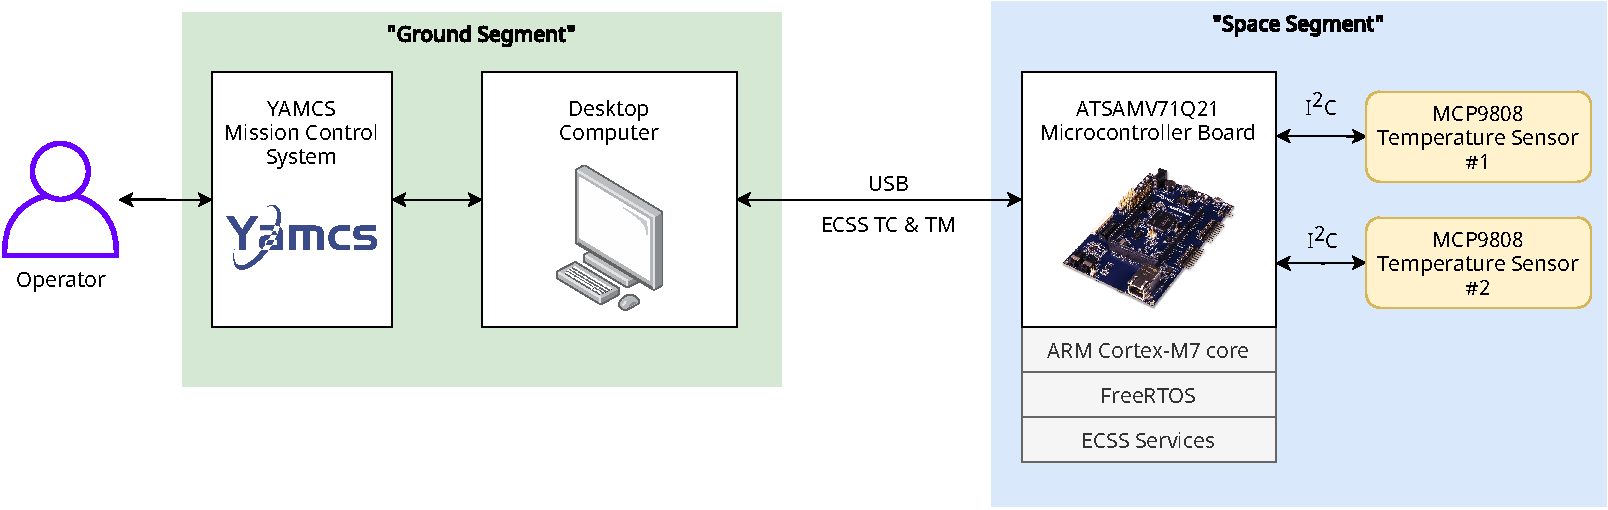
\includegraphics{SystemDescription}
	\caption{Μπλοκ διάγραμμα υψηλού επιπέδου της πειραματικής διάταξης}
	\label{fig:block}
\end{figure*}
\section{Περιγραφή Συστήματος}

\subsection{Λειτουργικότητα}
\label{sec:tsvcd}

Προκειμένου να εξομοιώσουμε τις πιο βασικές λειτουργίες ενός υποσυστήματος διαστημικού σκάφους, υλοποιήσαμε ένα σύστημα με μία μόνο λειτουργική προδιαγραφή:
\begin{quote}
	\texttt{RQ-010}: Το σύστημα πρέπει να μετρά και να μεταδίδει τη θερμοκρασία περιβάλλοντος.
\end{quote}

Προκειμένου να δικαιολογήσουμε μια υλοποίηση \ac{FDIR} για αυτό το σύστημα, θα εισάγουμε μια προδιαγραφή αξιοπιστίας:
\begin{quote}
	\texttt{RQ-020}: Καμία μεμονωμένη αποτυχία σε κάποιο μετρητικό στοιχείο δεν πρέπει να οδηγήσει σε απώλεια της λειτουργικότητας του συστήματος
\end{quote}

Ο λεπτομερής σχεδιασμός αυτού του απλού συστήματος επίδειξης παρουσιάζεται στις επόμενες ενότητες, και καταστρώθηκε έτσι ώστε να ταιριάζει όσο το δυνατόν περισσότερο με τη λειτουργικότητα, τις διεπαφές, το σχεδιασμό και το λογισμικό του νανοδορυφόρου AcubeSAT.

\begin{figure}
	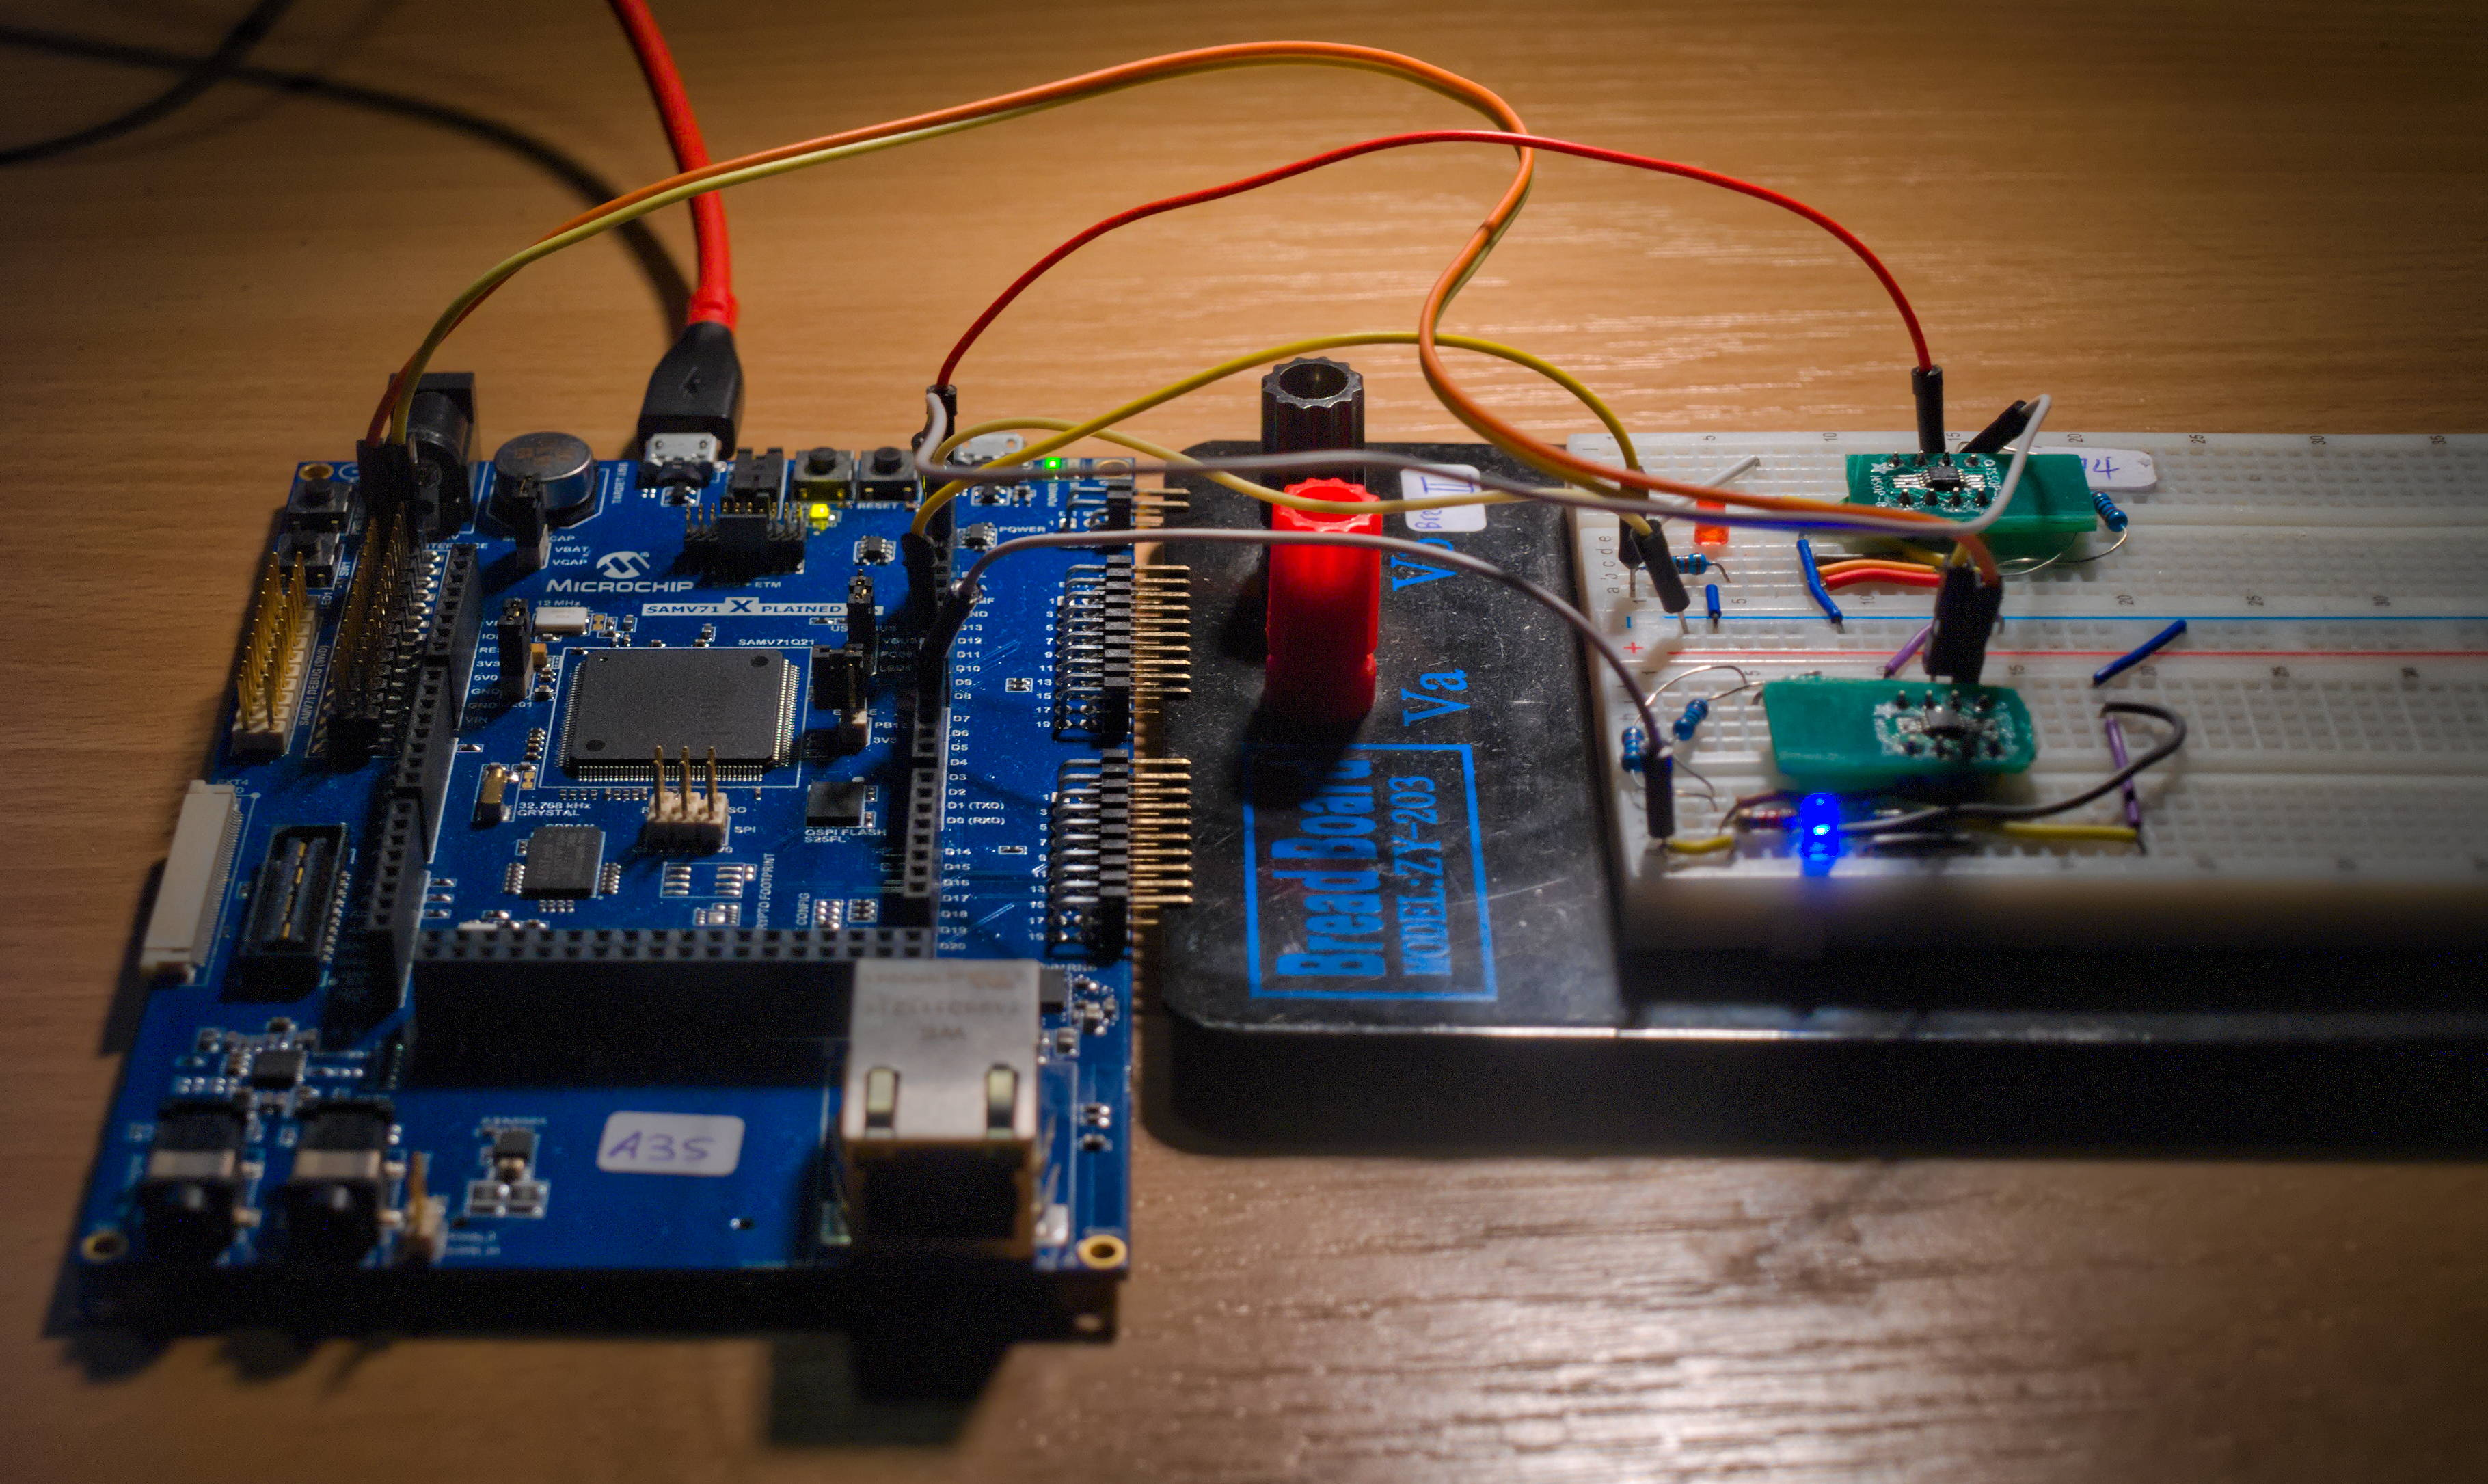
\includegraphics{test-system}\par
	\vspace*{3ex}
	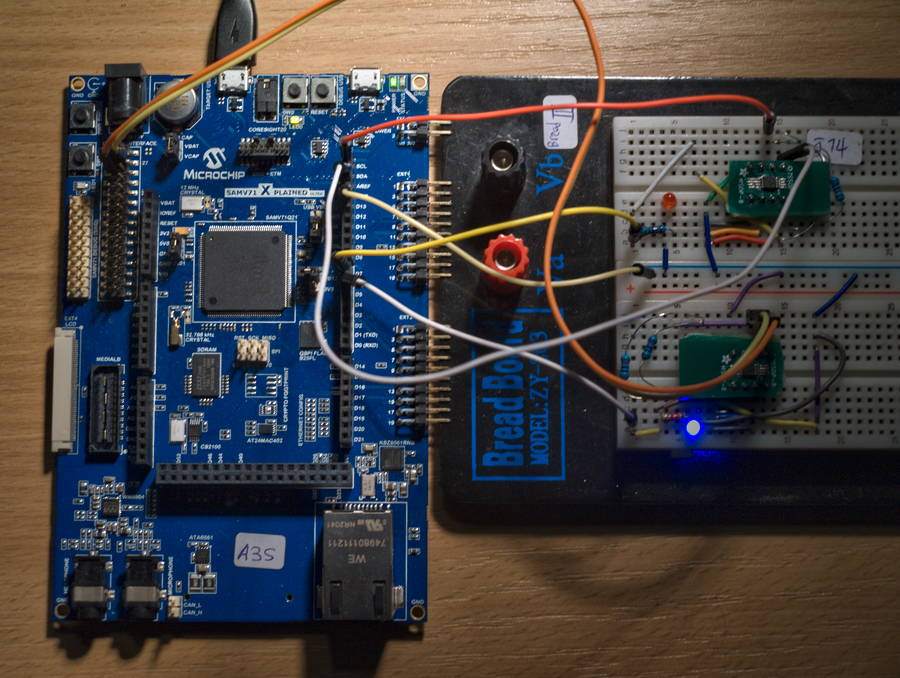
\includegraphics{system_top}
	\caption[Το πλήρες αναπτυξιακό σύστημα]{Το πλήρες δοκιμαστικό σύστημα. Αριστερά, διακρίνεται η μπλε αναπτυξιακή πλακέτα του μικροελεγκτή. Δεξιά βρίσκεται το breadboard, όπου οι είναι συνδεδεμένοι οι δύο αισθητήρες θερμοκρασίες. Διακρίνεται ακόμα η καλωδίωση από την πλακέτα προς το breadboard. Οι δύο ενδεικτικές λυχνίες δίνουν μία οπτική ένδειξη του αν το εξάρτημα λαμβάνει ισχύ ή όχι.}
\end{figure}

\subsection{Υλικό}

\begin{figure}
	\centering
	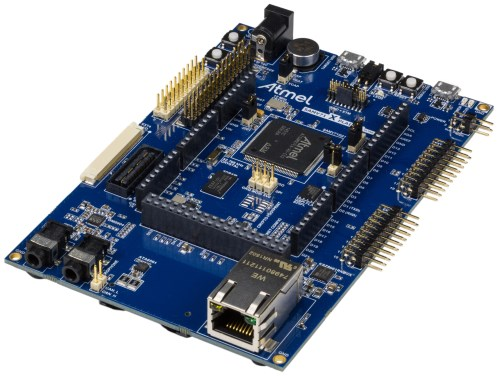
\includegraphics[width=.7\textwidth]{atsamv71xult}
	\caption{Επίσημη φωτογραφία της αναπτυξιακής πλακέτας ATSAMV71-XULT}
\end{figure}

Το κέντρο του συστήματος επίδειξης είναι ο \textbf{μικροελεγκτής} (\ac{MCU}) που χρησιμοποιείται για την προσομοίωση του σχεδιασμού και της λειτουργικότητας ενός από τα υποσυστήματα του AcubeSAT (\Cref{sec:obdh}). Ο επιλεγμένος μικροελεγκτής είναι ο Atmel \texttt{ATSAMV71Q21} που φιλοξενείται στην αναπτυξιακή πλακέτα \foothref{https://www.microchip.com/Developmenttools/ProductDetails/ATSAMV71-XULT}{\texttt{ATSAMV71-XULT}}. Αυτός ο μικροελεγκτής είναι λειτουργικά πανομοιότυπος με αυτόν που θα χρησιμοποιηθεί στην τροχιά, διαθέτοντας έναν 32-bit πυρήνα ARM Cortex-M7 με μνήμες \SI{2}{\mebi\byte} flash και \SI{384}{\kibi\byte} \acs{SRAM}, και μέγιστη ταχύτητα ρολογιού \SI{300}{\mega\hertz}.

\begin{marginfigure}
	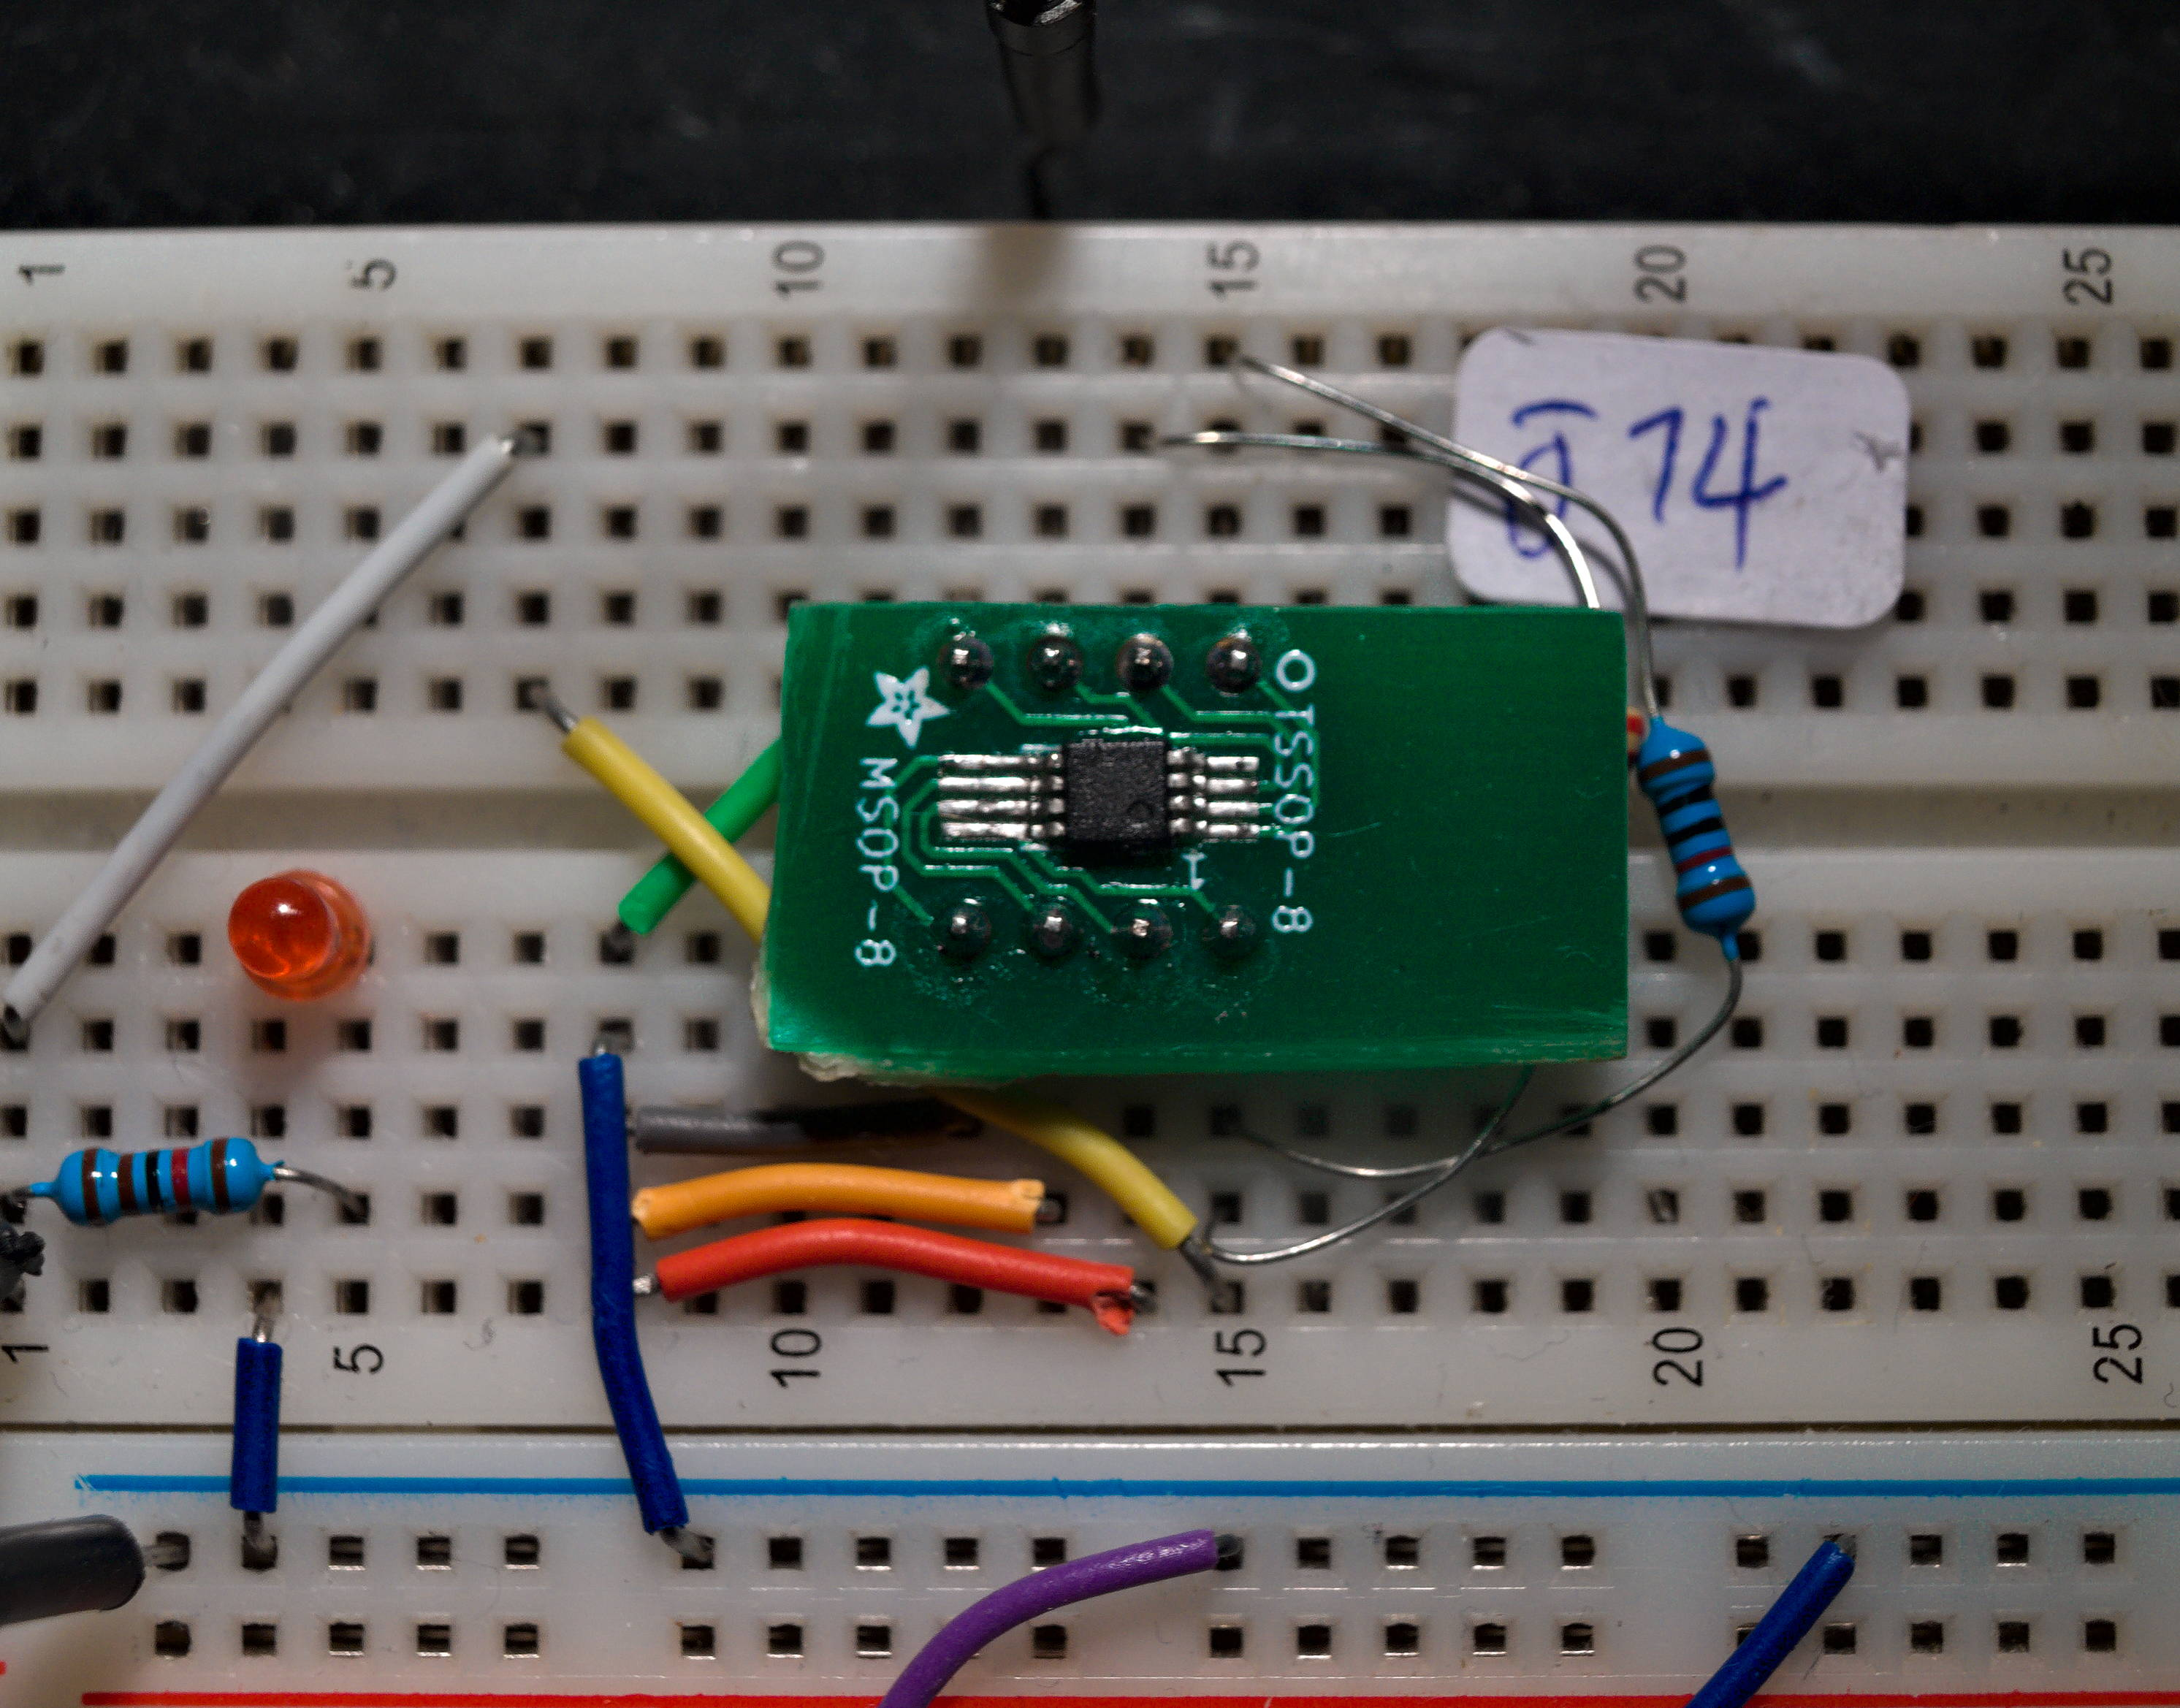
\includegraphics{mcp9808}
	\caption{Ο αισθητήρας θερμοκρασίας MCP9808, κολλημένος επάνω στην πλακέτα του πειράματος}
\end{marginfigure}

Ο μικροελεγκτής συνδέεται με δύο \textbf{αισθητήρες θερμοκρασίας} οι οποίοι χρησιμοποιούνται για την προσομοίωση εξαρτημάτων του υποσυστήματος που είναι επιρρεπή σε βλάβες. Οι επιλεγμένοι αισθητήρες είναι οι \foothref{https://www.microchip.com/wwwproducts/en/MCP9808}{\texttt{MCP9808}} της Microchip, οι οποίοι προσφέρουν ακριβή και ταχεία ανάγνωση της θερμοκρασίας μέσω ενός διαύλου \ac{I2C}. Η μέγιστη δυνατή περίοδος δειγματοληψίας για τον αισθητήρα είναι \SI{250}{\milli\second}.

\marginnote{%
\textbf{Ψυχρός πλεονασμός} (cold redundancy): Μόνο το ένα εξάρτημα λειτουργεί, ενώ τα άλλα όχι.

\textbf{Θερμός πλεονασμός} (warm redundancy): Ένα εξάρτημα λειτουργεί πλήρως, ενώ τα άλλα έχουν μειωμένη λειτουργικότητα.

\textbf{Ενεργός πλεονασμός} (hot redundancy): Δύο ή περισσότερα ταυτόχρονα ενεργά εξαρτήματα λειτουργούν παράλληλα \autocite{SAVOIR-HB-003}.
}

Οι δύο αισθητήρες είναι συνδεδεμένοι σε διάταξη \textbf{ενεργού πλεονασμού}, λόγω της εξαιρετικά χαμηλής ισχύος λειτουργίας τους. Οι δύο αισθητήρες είναι συνδεδεμένοι σε διαφορετικούς διαύλους \ac{I2C}, έτσι ώστε πιθανή βλάβη του ενός διαύλου να μην επηρεάζει τη λειτουργία του άλλου αισθητήρα.

\paragraph{Διεπαφή \acs{USB}} Για τη λήψη \acl{TM} και τη μετάδοση \acl{TC} στο υποσύστημα επίδειξης, ο σχεδιασμός περιλαμβάνει μια σύνδεση \acl{USB} με έναν τυπικό υπολογιστή. Η σύνδεση αυτή χρησιμοποιεί το περιφερειακό \acs{UART} του μικροελεγκτή, το οποίο μεταφέρει αποκλειστικά μηνύματα \acs{ECSS} \g{μεταξύ του μικροελεγκτή και του υπολογιστή. Τα μηνύματα αυτά περιλαμβάνουν τις τυπικές αναφορές} \acs{TM} και τα αιτήματα \acs{TC}, αλλά και μηνύματα καταγραφής που προορίζονται για διαγνωστικούς σκοπούς.

Καθώς το πρωτόκολλο \acs{UART} δεν προσφέρει κάποιο μηχανισμό για διαχωρισμό πακέτων, εφαρμόζουμε κωδικοποίηση \acs{COBS} \autocite{cheshire_consistent_overhead_1997} για όλα τα μεταδιδόμενα μηνύματα.

\begin{figure*}[h]
	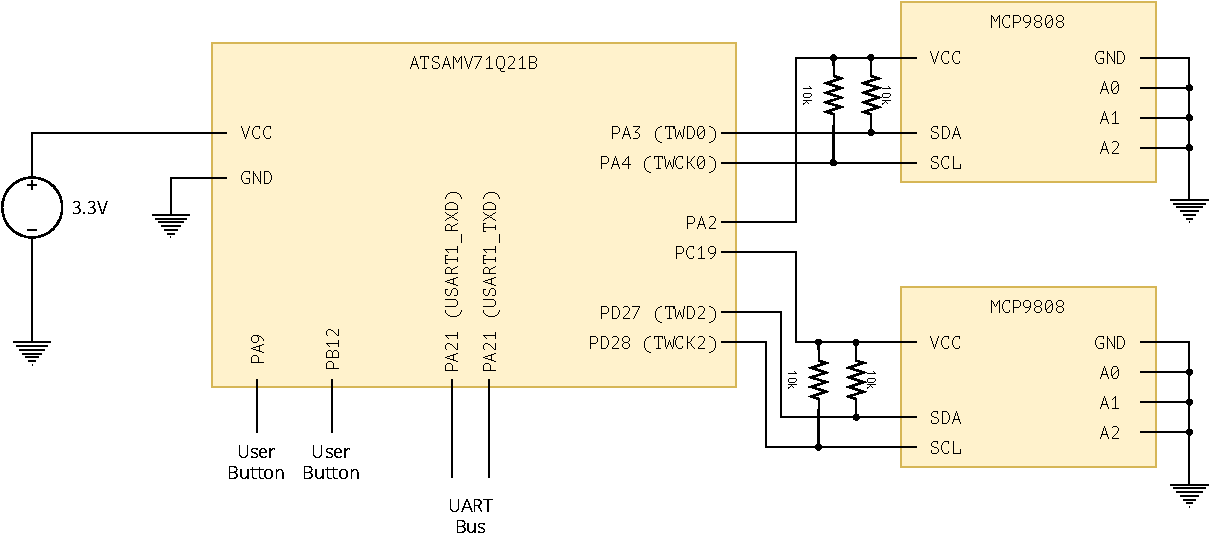
\includegraphics{ElectricalSchematic}
	\caption[Απλοποιημένο σχήματικό της εφαρμογής]{\g{Απλοποιημένο σχηματικό της εφαρμογής. Οι δύο αισθητήρες είναι συνδεδεμένοι μέσω} \ac{I2C} \g{με τις απαραίτητες αντιστάσεις ανύψωσης στα \SI{3.3}{\volt}. Η τροφοδοσία τους ελέγχεται απευθείας από τις εξόδους του μικροελεγκτή, επιτρέποντας στο χρήστη να τους αποσυνδέσει εντελώς αν χρειαστεί. Οι ακροδέκτες} \texttt{A} \g{των αισθητήρων ρυθμίζονται αυθαίρετα ώστε να επιλέγεται η διεύθυνση} \ac{I2C} \g{της κάθε συσκευής. Χρησιμοποιήσαμε την ίδια διεύθυνση, καθώς οι δύο δίαυλοι} \ac{I2C} \g{είναι πλήρως ανεξάρτητοι. Πυκνωτές αποσύζευξης, κρύσταλλοι και άλλα παθητικά εξαρτήματα δεν φαίνονται, καθώς περιλαμβάνονται ήδη στην έτοιμη αναπτυξιακή πλακέτα.}}
	\label{fig:schematic}
\end{figure*}

\paragraph{Συνδέσεις}
Η πλακέτα ανάπτυξης και οι αισθητήρες τοποθετήθηκαν και συνδέθηκαν χρησιμοποιώντας ένα breadboard. Τα ολοκληρωμένα κυκλώματα κολλήθηκαν επάνω σε απλές πλακέτες μικρού μεγέθους, που κατασκευάστηκαν με βάση το σχέδιο του Jaroslav Sýkora.\footnote[][9cm]{\url{https://bit.ly/3vZwuh1}}

\section{Λογισμικό}

\subsection{Δορυφορικό Κομμάτι}

Όλες οι λειτουργίες του \ac{FDIR} αναπτύχθηκαν χρησιμοποιώντας τη γλώσσα \textbf{C++}.

Επιλέχθηκε το μοντέρνο πρότυπο \texttt{C++17}. Ολόκληρη η εργασία βασίζεται σε ελεύθερο και ανοικτό λογισμικό το οποίο διατίθεται ελεύθερα για λήψη και τροποποίηση. Όλος ο κώδικας αναπτύχθηκε σε \foothref{https://git-scm.com/}{Git}.
	
	Η λειτουργικότητα του \ac{FDIR} \g{είναι δομημένη γύρω από την υλοποίηση του} \textbf{ECSS-E-ST-70-41C \ac{PUS} που γράφτηκε από την ομάδα AcubeSAT}\footnote{\url{https://gitlab.com/acubesat/obc/ecss-services}}, η οποία προσφέρει μια παραμετροποιήσιμη υλοποίηση του προτύπου χρησιμοποιώντας σύγχρονη C++.
	
	Το λογισμικό του μικροελεγκτή και η βασική λογική βασίζονται στο \textbf{\foothref{https://www.freertos.org/}{Free\acs{RTOS}}}, ένα λειτουργικό σύστημα πραγματικού χρόνου με χαμηλές απαιτήσεις που απευθύνεται σε ενσωματωμένες συσκευές. Το FreeRTOS παρέχει ανεξάρτητες διεργασίες και δομές που επιτρέπουν τον ασφαλή συγχρονισμού δεδομένων μεταξύ παράλληλων παραγωγών \& καταναλωτών.
\begin{figure*}[h]
	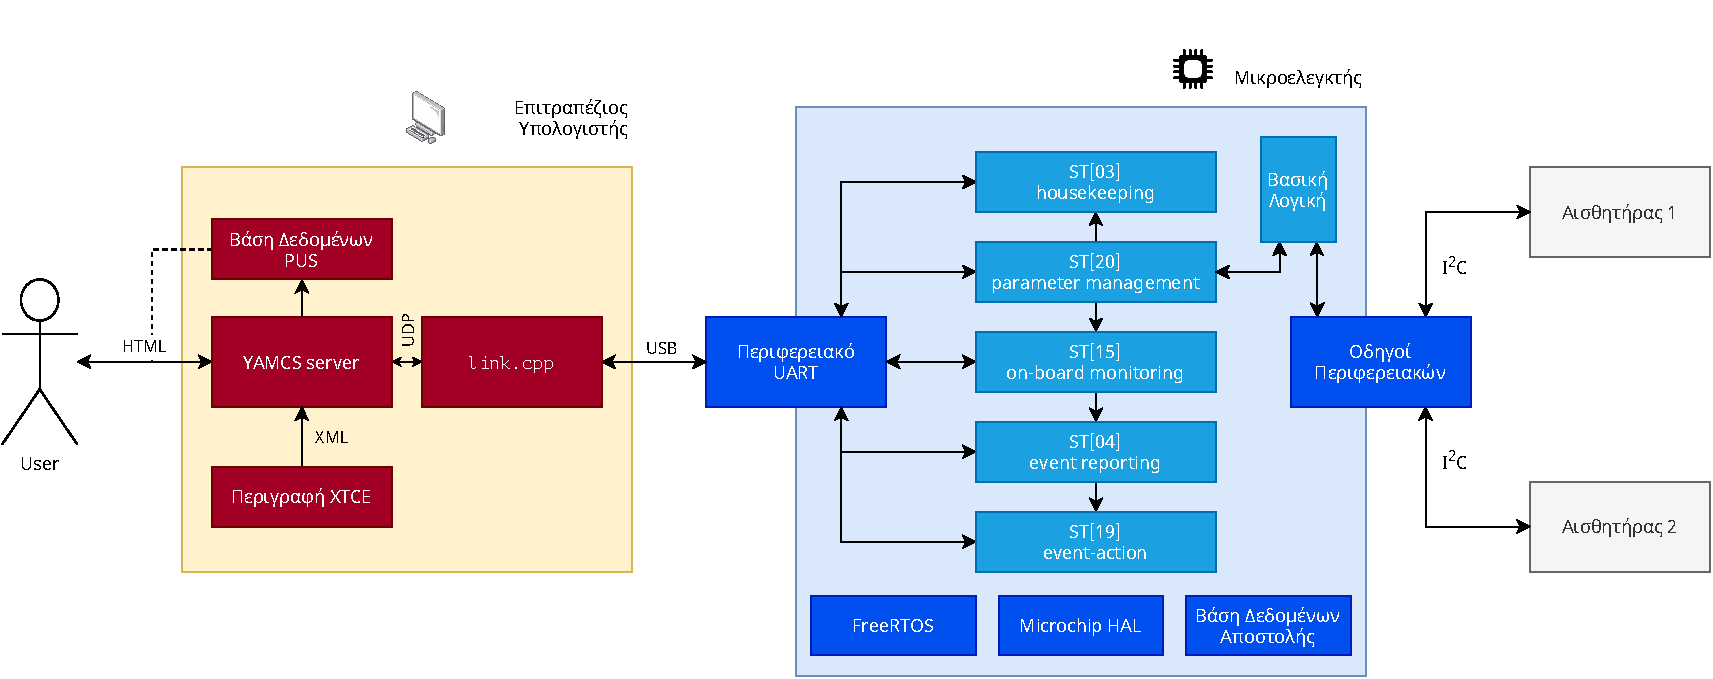
\includegraphics{SoftwareFlow-el}
	\caption{Η ροή δεδομένων μεταξύ των διαφορετικών κομματιών του λογισμικού}
	\label{sec:softwareflow}
\end{figure*}

\begin{table*}[h]
	\centering
	\caption[][5pt]{Λίστα διεργασιών του Free\acs{RTOS} που υλοποιούν την πειραματική διάταξη}
	\label{tab:rtos-tasks}
	\renewcommand{\arraystretch}{1.5}
	\begin{tabularx}{\textwidth}{@{}llX@{}}
		\toprule
		Όνομα & Μέγεθος στοίβας & Επεξήγηση \\ \midrule
		\texttt{Internal\_Temp} & \SI{2.5}{\kilo\byte} & Λαμβάνει διαγνωστικές μετρήσεις από τον εσωτερικό αισθητήρα θερμοκρασίας του μικροελεγκτή, και αναβοσβήνει ένα LED για σκοπούς παρατηρησιμότητας. \\
		\texttt{ECSS} & \SI{3}{\kilo\byte} & Εκτελεί τις περιοδικές διαδικασίες που ορίζουν οι υπηρεσίες \acs{ECSS}. Αυτό περιλαμβάνει την εκπομπή ραδιοφάρων και τον έλεγχο των ορισμών παρακολούθησης. Αυτή η διεργασία υλοποιεί το \acs{FDIR}. \\
		\texttt{\acs{UART}\_Tx} & \SI{3}{\kilo\byte} & Αποστολή μηνυμάτων προς τον υπολογιστή. Η διεργασία αυτή λειτουργεί ως "gatekeeper task", δηλαδή είναι η μόνη διεργασία που μπορεί να στείλει μηνύματα \acs{UART}. Όλες οι άλλες διεργασίες επικοινωνούν με αυτήν μέσω μίας στοίβας. \\
		\texttt{\acs{UART}\_Rx} & \SI{6}{\kilo\byte} & Λήψη μηνυμάτων \acs{UART} από τον υπολογιστή. Για απλότητα, αυτή η διεργασία, πέρα από λήψη τηλεεντολών, πραγματοποιεί και την άμεση εκτέλεσή τους. \\
		\texttt{T1} & \SI{1.5}{\kilo\byte} & Επικοινωνία με τον αισθητήρα θερμοκρασίας 1, και ενημέρωση των αντίστοιχων παραμέτρων \\
		\texttt{T2} & \SI{1.5}{\kilo\byte} & Επικοινωνία με τον αισθητήρα θερμοκρασίας 2, και ενημέρωση των αντίστοιχων παραμέτρων \\ \bottomrule
	\end{tabularx}
\end{table*}

Για να διασφαλιστεί υψηλή αξιοπιστία και χαμηλή κατανάλωση πόρων, οι ακόλουθοι \textbf{περιορισμοί} λαμβάνονται υπ' όψιν την ανάπτυξη σε C++:
\begin{compactenum}
	\item Η δυναμική κατανομή μνήμης\footnote{Χρήση των \mintinline{cpp}{malloc}, \mintinline{cpp}{new} κλπ.} απαγορεύεται εντελώς.
	\label{itm:malloc}
	\item Το \Cref{itm:malloc} σημαίνει ότι οι κλασικές δομές δεδομένων της C++\footnote{\mintinline{cpp}{std::vector}, \mintinline{cpp}{std::string}, \mintinline{cpp}{std::map} κλπ.} δεν μπορούν να χρησιμοποιηθούν. Αντίθετα, η βιβλιοθήκη \foothref{https://www.etlcpp.com/}{\acf{ETL}} περιλαμβάνει δομές που αποθηκεύονται σε στατική μνήμη, ή στην στοίβα.
	\item "Ακριβά" χαρακτηριστικά, όπως το \emph{Run-Time Type Inference}, οι δυναμικές μετατροπές τύπων (dynamic casts) ή οι εξαιρέσεις (exceptions) απαγορεύονται επίσης.
\end{compactenum}

Η βιβλιοθήκη \ac{HAL} και η σουίτα λογισμικού \foothref{https://www.microchip.com/en-us/development-tools-tools-and-software/embedded-software-center/mplab-harmony-v3}{MPLAB Harmony}  χρησιμοποιούνται για την επικοινωνία με όλα τα ενσωματωμένα περιφερειακά του μικροελεγκτή. Το \foothref{https://www.jetbrains.com/clion/}{CLion} έχει επιλεγεί ως το \acs{IDE}, μαζί με το σύστημα "χτισίματος" κώδικα \foothref{https://cmake.org/}{CMake}.

Όλο το λογισμικό που αναπτύχθηκε στο πλαίσιο της παρούσας διατριβής είναι διαθέσιμο στο διαδίκτυο και έχει καταγραφεί στον \Cref{tab:new_software}. Τα πιο κρίσιμα μέρη του λογισμικού που αναπτύχθηκε έχουν αναπαραχθεί στο \Cref{sec:source_code}. Μια λίστα των έτοιμων ή τροποποιημένων βιβλιοθηκών που χρησιμοποιήθηκαν μπορεί επίσης να βρεθεί στον \Cref{tab:old_software}.


\begin{table*}[h]
	\centering
	\caption[][5pt]{Λίστα του νέου λογισμικού που αναπτύχθηκε για την παρούσα εργασία}
	\label{tab:new_software}
	\begin{tabularx}{\textwidth}{@{}lXp{6cm}@{}}
		\toprule
		Όνομα & Περιγραφή & URL \\ \midrule
		\textbf{\texttt{fdir-demo}} & Πλήρης κώδικας για τον μικροελεγκτή  & \small \url{https://github.com/kongr45gpen/fdir-demo} \\
		\textbf{\texttt{fdir-demo-yamcs}} & Λογισμικό Σταθμού Βάσης: \begin{enumerate}
			\item Διεπαφή με το \acs{YAMCS}
			\item Περιγραφή \acs{ECSS} πακέτων, αναγνώσιμη από μηχανή
			\item Διεπαφή \acs{UART}--\acs{USB} με τον μικροελεγκτή
			\item Πρόγραμμα εμφάνισης της βάσης δεδομένων \acs{PUS}\vspace*{-2ex}
			\end{enumerate} & \small \url{https://github.com/kongr45gpen/fdir-demo-yamcs} \\
		\bottomrule
	\end{tabularx}
\end{table*}

\begin{table*}[h]
	\centering
	\vspace{2em}
	\caption[][5pt]{Λίστα των έτοιμων βιβλιοθηκών που χρησιμοποιήθηκαν}
	\renewcommand{\arraystretch}{1.5}
	\label{tab:old_software}
	\begin{tabularx}{\textwidth}{@{}lp{6cm}X@{}}
		\toprule
		Όνομα & Περιγραφή & Μεταβολές \\ \midrule
		\href{https://www.freertos.org/}{FreeRTOS} & Λειτουργικό σύστημα πραγματικού χρόνου & \\
		\href{https://gitlab.com/acubesat/obc/ecss-services}{\texttt{ecss-services}} & C++ υλοποίηση του προτύπου ECSS-E-ST-70-41C %\autocite{ECSS-E-ST-70-41C} 
		& \small
		Προστέθηκαν υλοποιήσεις υπηρεσιών που δεν υπήρχαν, και βελτιώθηκαν συναρτήσεις διεπαφής με τον μικροελεγκτή\newline\small\url{https://gitlab.com/kongr45gpen/ecss-services/-/tree/fdir}
		 \\
		 \href{https://www.etlcpp.com/}{\acs{ETL}}  & Βιβλιοθήκη C++ (περιλαμβάνει δομές δεδομένων, αλγορίθμους και άλλα εξαρτήματα) για κρίσιμες εφαρμογές με περιορισμένη μνήμη &
		 \\
 		\href{https://github.com/yamcs/yamcs}{\acs{YAMCS}}  & Σουίτα λογισμικού για έλεγχο διαστημικών αποστολών& %\autocite{cheshire_consistent_overhead_1997}
 		\\
		\href{https://github.com/cmcqueen/cobs-c}{\texttt{cobs-c}}  & Υλοποίηση του πρωτοκόλλου \ac{COBS} %\autocite{cheshire_consistent_overhead_1997}
		 & \\
		 \href{https://getmdl.io/}{Material Design Lite}  & Σουίτα έτοιμων σχεδιαστικών στοιχείων σε γλώσσα CSS (για σταθμό βάσης)
		 & \\
		 \href{https://lodash.com/}{\texttt{lodash}}  & Βοηθητικές συναρτήσεις σε Javascript (για σταθμό βάσης)
		 & \\
		\bottomrule
	\end{tabularx}
\end{table*}

\FloatBarrier
\subsection{Μέγεθος Λογισμικού}
\g{Καθώς αναπτύσουμε ένα ενσωματωμένο σύστημα σε μικροελεγκτή με περιορισμούς χώρου, έχει νόημα η ανάλυση του μεγέθους του κώδικα που παράγεται. Ο μεταγλωττιστής \texttt{gcc} παρέχει τη δυνατότητα μέτρησης των καταναλισκόμενων πόρων. Το συνολικό μέγεθος του προγράμματος παρουσιάζεται στον \Cref{tab:resusage}, και τα αρχεία} C++ με την μεγαλύτερη κατανάλωση μνήμης λογισμικού και μνήμης δεδομένων φαίνονται στους \Cref{tab:ramusage,tab:romusage}.\footnote{Τα δεδομένα παρήχθησαν με χρήση της βιβλιοθήκης \href{https://github.com/PromyLOPh/linkermapviz}{\texttt{linkermapviz}}.}

\begin{table}[h]
	\centering
	\caption{Μέγεθος του παραχθέντος κώδικα με διαφορετικές ρυθμίσεις μεταγλωττιστή}
	\label{tab:resusage}
	\begin{tabular}{@{}llll@{}}
		\toprule
		\multicolumn{4}{l}{Κώδικας χωρίς βελτιστοποίηση (\texttt{-O0})} \\ \midrule
		Περιοχή μνήμης &        Χρησιμοποιημένη & Συνολικό μέγεθος &  Ποσοστό \\[1ex]
		\acs{ROM}   &   \SI{254324}{\byte}   &    \SI{  2}{\mega\byte} &     12.13\% \\
		\acs{RAM}   &   \SI{205992}{\byte}   &    \SI{384}{\kilo\byte} &     52.39\% \\ \midrule
		\multicolumn{4}{l}{Βελτιστοποίηση ελάχιστου μεγέθους (\texttt{-Ofast})} \\ \midrule
		Περιοχή μνήμης &        Χρησιμοποιημένη & Συνολικό μέγεθος &  Ποσοστό \\[1ex]
		\acs{ROM}   &   \SI{228384}{\byte}   &    \SI{  2}{\mega\byte} &     10.89\% \\
		\acs{RAM}   &   \SI{205992}{\byte}   &    \SI{384}{\kilo\byte} &     52.39\% \\ \bottomrule
	\end{tabular}
	\vspace{2ex}
	\setfloatalignment{b}
\end{table}

\begin{table}[h]
	\centering
	\caption[Τα αρχεία που καταναλώνουν την περισσότερη μνήμη ROM]{Τα αρχεία που καταναλώνουν την περισσότερη μνήμη \acs{ROM} (δεν περιλαμβάνονται βιβλιοθήκες συστήματος)}
	\label{tab:romusage}
	\begin{tabularx}{\textwidth}{@{}S[table-format=5.0]X@{}}
		\toprule
		Μέγεθος (\si{\byte}) & Αρχείο \\ \midrule
		22515 & \texttt{ServicePool.cpp} \\
		12350 & \texttt{main.cpp} \\
		9271 & \texttt{TimeBasedSchedulingService.cpp} \\
		8684 & \texttt{SystemParameters.cpp} \\
		7708 & \texttt{EventActionService.cpp} \\
		6546 & \texttt{OnBoardMonitoringService.cpp} \\
		5952 & \texttt{ECSSTask.cpp} \\
		4451 & \texttt{FreeRTOS\_tasks.c} \\
		4404 & \texttt{MCP9808-internal.cpp} \\
		3281 & \texttt{Logger.cpp} \\
		\bottomrule
	\end{tabularx}
	\vspace{2ex}
	\setfloatalignment{b}
\end{table}

\begin{table}[h]
	\centering
	\caption[Τα αρχεία που καταναλώνουν την περισσότερη μνήμη RAM]{Τα αρχεία που καταναλώνουν την περισσότερη μνήμη \acs{RAM} (δεν περιλαμβάνονται βιβλιοθήκες συστήματος)}
	\label{tab:ramusage}
	\begin{tabularx}{\textwidth}{@{}S[table-format=5.0]X@{}}
		\toprule
		Μέγεθος (\si{\byte}) & Αρχείο \\ \midrule
		131104 & \texttt{heap\_4.c} \\
		38088 & \texttt{ServicePool.cpp} \\
		11192 & \texttt{UARTTask.cpp} \\
		1064 & \texttt{SystemParameterMonitoring.cpp} \\
		340 & \texttt{UARTRXTask.cpp} \\
		260 & \texttt{FreeRTOS\_tasks.c} \\
		200 & \texttt{sys\_time.c} \\
		188 & \texttt{SystemParameters.cpp} \\
		50 & \texttt{main.cpp} \\
		\bottomrule
	\end{tabularx}
\end{table}

\vspace{2ex}

\g{Να σημειωθεί πως δεν έχει γίνει καμία προσπάθεια για βελτιστοποίηση της κατανάλωσης μνήμης ή γενικότερα των επιδόσεων του συστήματος. Επίσης, να τονιστεί πως λόγω της χρήσης της βιβλιοθήκης} \acs{ETL} \g{και της έλλειψης δυναμικής κατανάλωσης μνήμης, οι καταναλώσεις του \Cref{tab:ramusage} αναφέρονται στην πλειοψηφία σχεδόν της κατανάλωσης μνήμης} \acs{RAM}. \g{Μάλιστα, η στοίβα} (stack) \g{όπου αρχικοποιούν μεταβλητές οι διεργασίες του} FreeRTOS, \g{είναι καταχωρημένη εξ' ολοκλήρου στο αρχείο} \texttt{heap\_4.c}.

\FloatBarrier
\subsection{Εντοπισμός Αποτυχιών \acs{I2C}}
\label{sec:howcani2cfail}


Έχει ενδιαφέρον να μελετήσουμε πώς το περιφερειακό \ac{I2C} \g{του μικροελεγκτή μπορεί να χρησιμοποιηθεί για τον εντοπισμό διαφόρων ειδών σφαλμάτων στον δίαυλο και τα περιφερειακά:}

\begin{enumerate}
	\item \textbf{Σφάλματα περιφερειακού}
	
	\marginnote{Για να εξασφαλιστεί ο εντοπισμός των σφαλμάτων του περιφερειακού, είναι σημαντικό να βεβαιωθούμε ότι η κατάσταση σφάλματος του περιφερειακού αναγιγνώσκεται μετά από κάθε επικοινωνία. Τα interrupts του μικροελεγκτή και η εντολή \href{https://en.cppreference.com/w/cpp/language/attributes/nodiscard}{\mintinline{cpp}{[[nodiscard]]}} της C++ συνδυάζονται για να διασφαλιστεί ότι όλα τα σφάλματα του υλικού λαμβάνονται υπ' όψιν.}
	Το περιφερειακό \ac{I2C} του μικροελεγκτή είναι ικανό να παράγει σφάλμα κάθε φορά που \emph{το συνδεδεμένο περιφερειακό δεν θέτει το bit "acknowledge"}. Η αποτυχία να θέσει αυτό το bit μπορεί να είναι αποτέλεσμα αποσύνδεσης των γραμμών ρολογιού (\acs{SCL}) ή δεδομένων (\acs{SDA}), βλάβης του διαύλου ή κακής λειτουργίας του ίδιου του περιφερειακού.
	
	\item \textbf{Χρονικό περιθώριο απάντησης}
	
	Σε ορισμένες δυσμενείς για το \ac{I2C} ηλεκτρικές συνθήκες, που μπορεί να προκληθούν από λανθασμένα επιλεγμένες τιμές αντίστασης pull-up ή μεγάλο χωρητικό φορτίο, η ακεραιότητα του σήματος \ac{I2C} μπορεί να χαθεί (\Cref{subfig:i2c_clean}). Αυτό το σφάλμα δεν ανιχνεύεται άμεσα από το περιφερειακό του μικροελεγκτή, αλλά μπορεί να διαγνωστεί με την προσθήκη ενός χρονικού ορίου (timeout) στις αναγνώσεις δεδομένων του αισθητήρα.
	
	\item \textbf{Chip ID}
	
	\begin{margintable}
		\centering
		\caption{Μη εγγράψιμοι καταχωρητές του MCP9808}
		\label{tab:mcp9808readonly}
		\begin{tabularx}{\linewidth}{@{}lXl@{}}
			\toprule
			Διεύ/ση & Καταχωρητής & Τιμή \\ \midrule
			\texttt{0x06} & Manufacturer ID & \texttt{0x0054} \\
			\texttt{0x07} & Device ID & \texttt{0x0400} \\ \bottomrule
		\end{tabularx}
	\end{margintable}

	Είναι πιθανό ο αισθητήρας να υποστεί σοβαρή βλάβη, αλλά να είναι ακόμα σε θέση να ανταποκριθεί στις εντολές \ac{I2C} ή να θέσει το bit \emph{acknowledge}. Για τον λόγο αυτό, πριν από κάθε ανάγνωση της θερμοκρασίας, πραγματοποιείται ένας πιο αυστηρός έλεγχος της κατάστασης του αισθητήρα: οι \emph{μόνιμοι} καταχωρητές του περιφερειακού περιέχουν τιμές οι οποίες, υπό κανονικές συνθήκες, δεν μπορούν να αλλάξουν εκτός αν υπάρξει βλάβη υλικού. Εάν επιστραφεί οποιαδήποτε τιμή διαφορετική από την αναμενόμενη, θεωρείται ότι το περιφερειακό ή ο δίαυλος έχει εμφανίσει σφάλμα.
\end{enumerate}

\begin{figure}[h]
	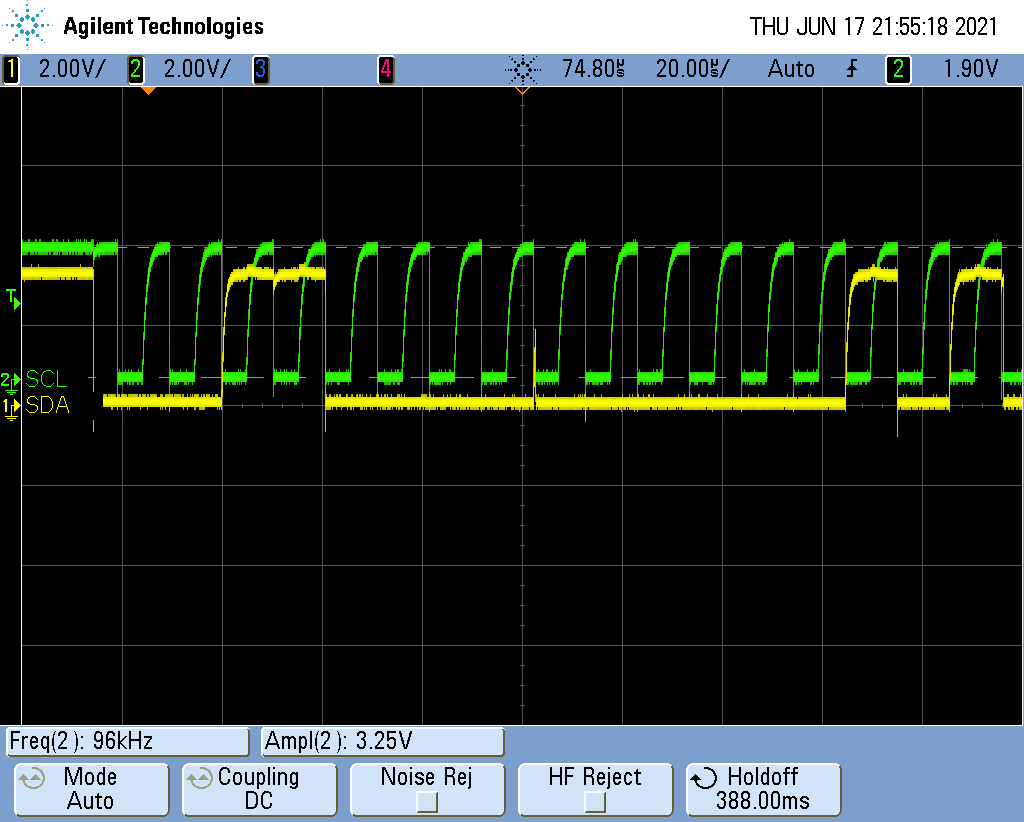
\includegraphics[trim={0 10cm 0 1.8cm},clip]{scope_1}
	\caption[Καθαρό σήμα \acs{I2C}]{Καθαρό σήμα \acs{I2C}. Η πράσινη κυματομορφή (\acf{SCL}) έχει σχήμα όπου μπορούν εύκολα να ξεχωριστούν οι παλμοί, και τα δεδομένα της κίτρινης κυματομορφής (\acf{SDA}) συνδέονται αντίστοιχα με τους παλμούς ρολογιού. Το πλάτος των κυματομορφών είναι περίπου \SI{3.3}{\volt}}
	\label{subfig:i2c_clean}
\end{figure}

\begin{figure}[h]
	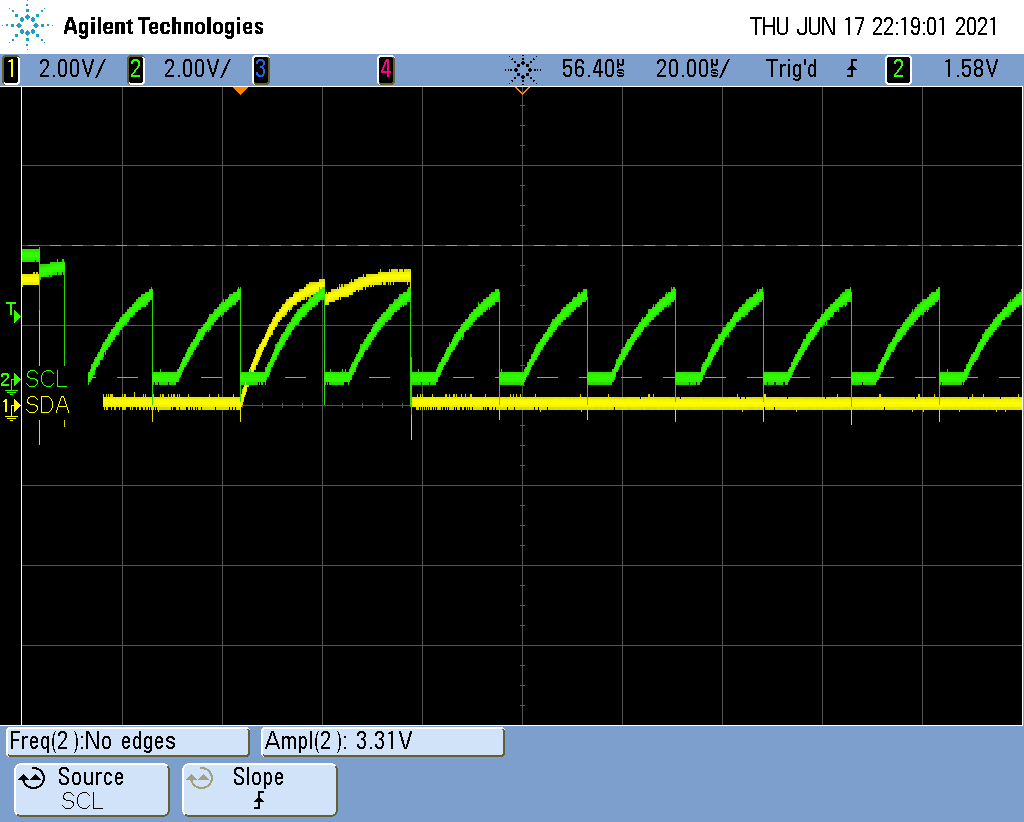
\includegraphics[trim={0 10cm 0 1.8cm},clip]{scope_5}
	\caption[Σήμα σε ένα ελαττωματικό δίκτυο \acs{I2C}]{Σήμα σε ένα ελαττωματικό δίκτυο \acs{I2C}, όπου υπάρχει πολύ μεγάλο χωρητικό φορτίο. Ο χρόνος ανόδου και των δύο σημάτων είναι υπερβολικά μεγάλος, και η επικοινωνία στη συγκεκριμένη συχνότητα δεν είναι δυνατή. Το σήμα δεν προλαβαίνει να φτάσει την τιμή των \SI{3.3}{\volt}. Σε αυτήν την περίπτωση, δεν είναι δυνατή η μεταφορά δεδομένων στον δίαυλο, και το δίκτυο ή το εξάρτημα θεωρείται πως έχει αποτύχει.}
	\label{subfig:i2c_dirty}
\end{figure}

\FloatBarrier

\subsection{Έλεγχος Αποστολής}

Ο υπολογιστής του επίγειου τμήματος πρέπει να αναλύει τα λαμβανόμενα πακέτα και να στέλνει εντολές, καθώς και να εμφανίζει πληροφορίες σχετικά με τις μετρήσεις των αισθητήρων, την κατάσταση του \ac{FDIR}, \g{και την υγεία του συνδεδεμένου συστήματος πτήσης.}

Η σουίτα λογισμικού \acs{YAMCS} \autocite{sela_yamcs_lightweight_2012} \g{επιλέχθηκε για να καλύψει τις παραπάνω ανάγκες, και προσαρμόστηκε ώστε να παρέχει τις δυνατότητες που απαιτούνται για την παρούσα επίδειξη}.

Το πρωτόκολλο \ac{ECSS} \autocite{ECSS-E-ST-70-41C} \g{δεν υποστηρίζεται εγγενώς από το \linebreak[4]}\acs{YAMCS}\g{. Ωστόσο, οι απαραίτητες εντολές έχουν εισαχθεί στο σύστημα μέσω αρχείων μορφής} \ac{XTCE} \autocite{simon_xtce_standard_2004}. Ο πηγαίος κώδικας της ενσωμάτωσης μπορεί να βρεθεί στο \Cref{app:xtce}.

\begin{figure}[h]
	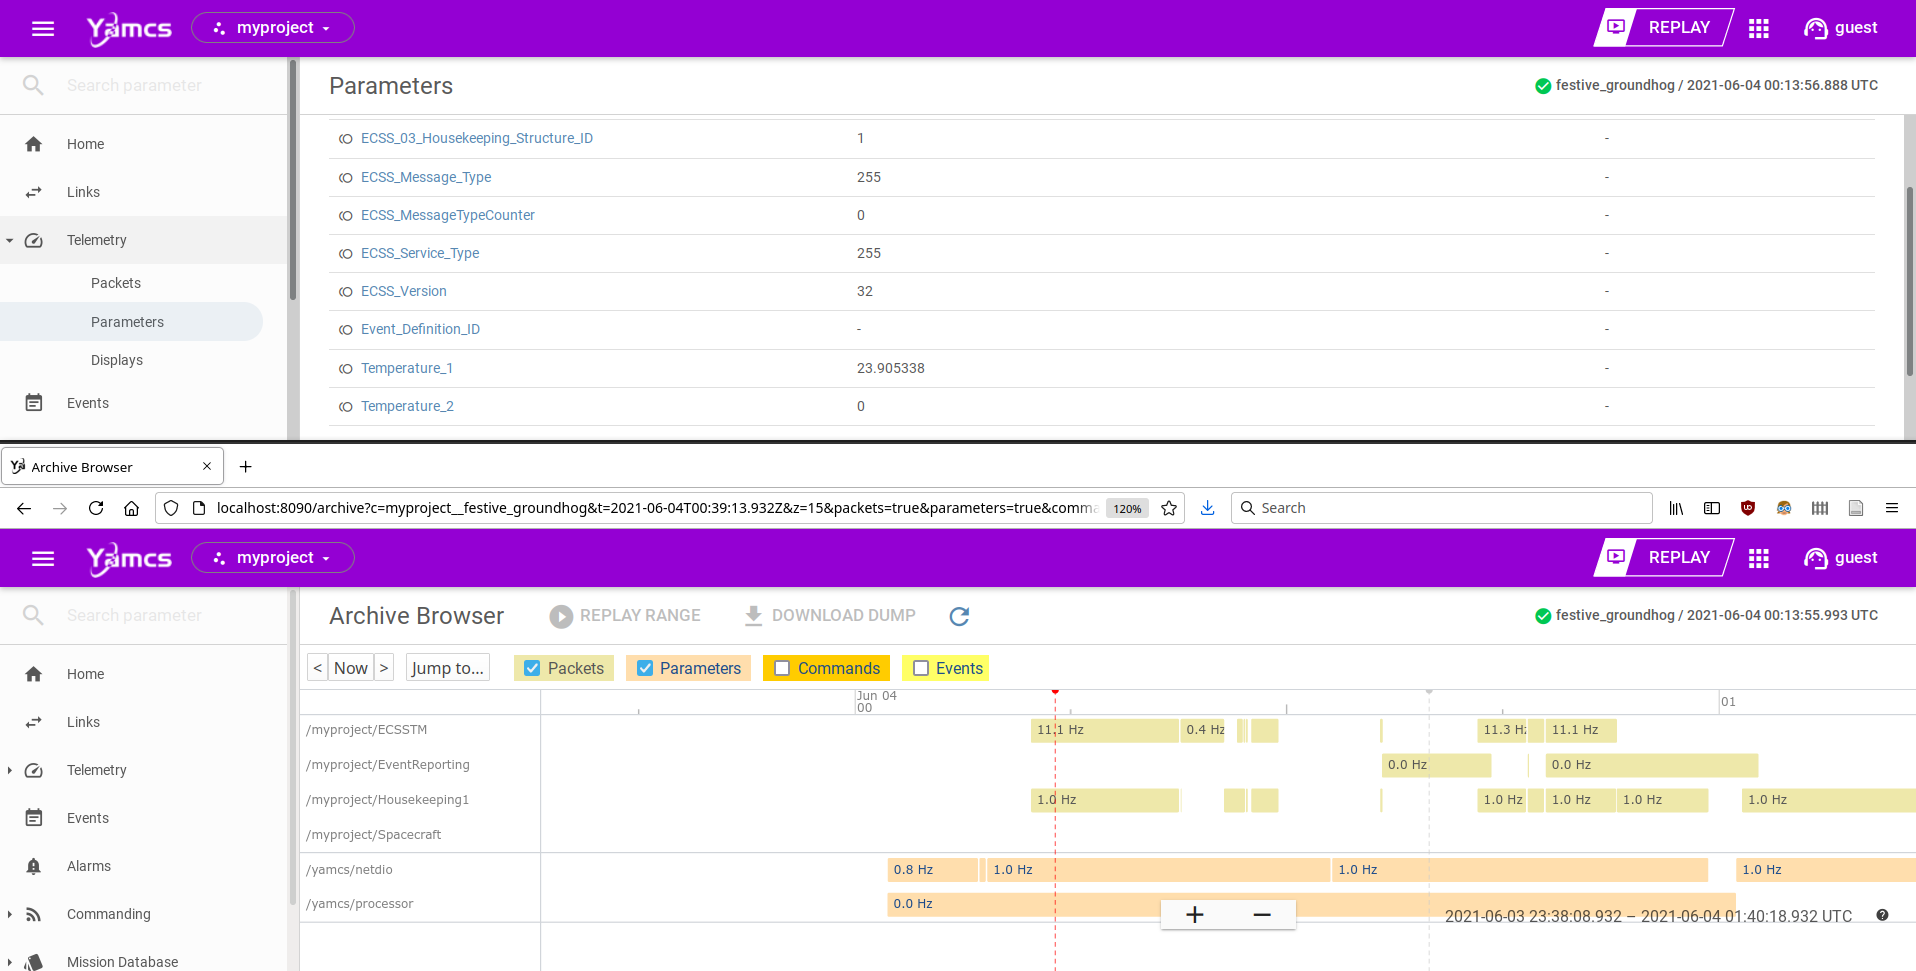
\includegraphics{screenshots/yamcs_replay}
	\caption{Προβολές παραμέτρων και αρχείου στο \acs{YAMCS}}
\end{figure}

\subsection{Βάση Δεδομένων \acs{PUS}}
\label{sec:pusinterface}

Η σουίτα \acs{YAMCS} δεν διαθέτει έτοιμη υποστήριξη και συγχρονισμό με τη βάση δεδομένων \acs{PUS} του δορυφόρου. Αυτό σημαίνει πως δεν υπάρχει έτομος εύκολος τρόπος για εποπτική προβολή των \emph{γεγονότων}, \emph{παραμέτρων}, ορισμών \emph{παρακολούθησης} και ορισμών \emph{γεγονότος-αντίδρασης}.

\begin{figure*}[h]
	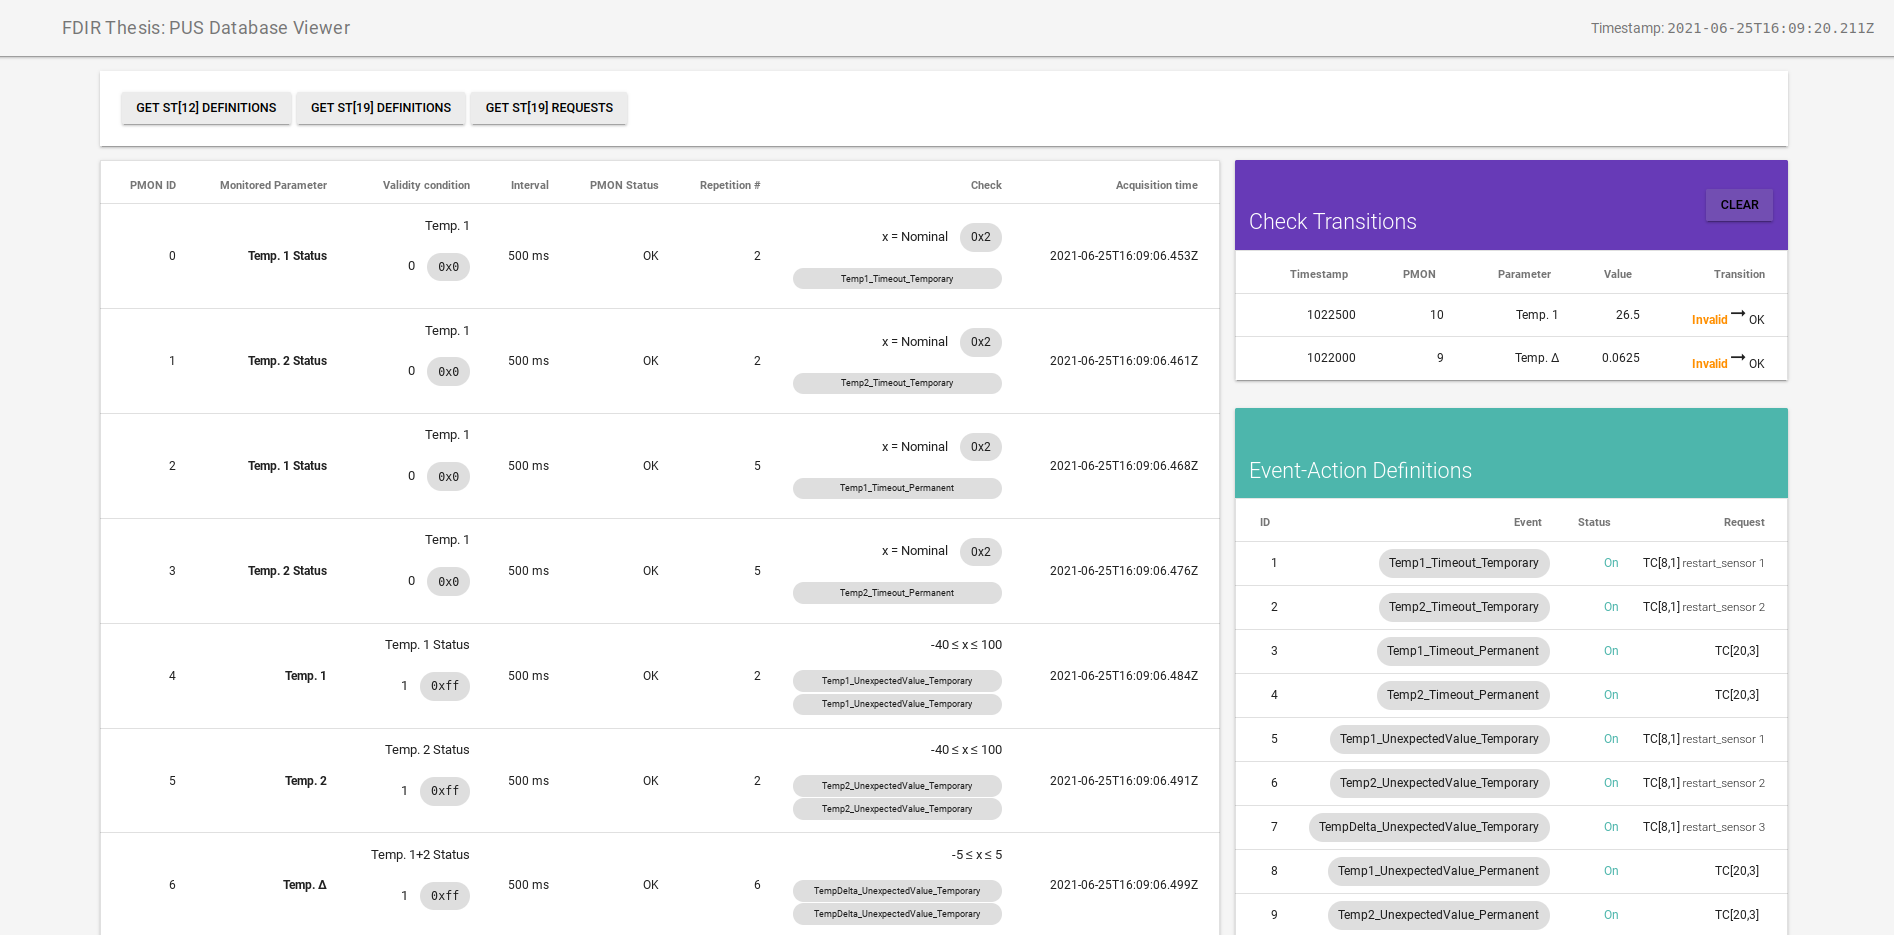
\includegraphics{screenshots/pus_viewer}
	\caption[Η διεπαφή "PUS database viewer"]{Η διεπαφή "\acs{PUS} database viewer". \g{Αριστερά βρίσκεται η λίστα ορισμών παρακολούθησης, πάνω δεξιά η λίστα μεταβάσεων, και κάτω δεξιά η λίστα ορισμών γεγονότος-αντίδρασης.}}
	\label{fig:pusviewer}
\end{figure*}

\g{Για να διευκολυνθεί η γρήγορη προβολή της διαδικασίας του} \acs{FDIR}, \g{υλοποιήσαμε μία} online \g{διεπαφή που δείχνει τα παραπάνω (\Cref{fig:pusviewer}). Η διεπαφή ενημερώνεται σε πραγματικό χρόνο μέσω του} \acs{YAMCS} \acs{HTTP} \acs{API} και προβάλλει τους ορισμούς αλλά και την κατάσταση του \acs{FDIR}.

Η εφαρμογή γράφτηκε σε HTML και Javascript, εκμεταλλευόμενη WebSockets, και το γραφικό περιβάλλον της βασίζεται στη βιβλιοθήκη Material Design Lite.\footnote[][3ex]{\url{https://getmdl.io/}} Βρίσκεται στο αποθετήριο \linebreak[4] \foothref{https://github.com/kongr45gpen/fdir-demo-yamcs/tree/master/ecss-interface}{\texttt{fdir-demo-yamcs}}, μαζί με τα υπόλοιπα κομμάτια του σταθμού βάσης της επίδειξης.


\section{Στήσιμο \acs{FDIR}}

\g{Ο σκοπός της πειραματικής διάταξης είναι να παρατηρηθεί η απόκριση του συστήματος σε τυχόν αποτυχία των δύο "ευπρόσβλητων" αισθητήρων θερμοκρασίας. Για το σκοπό αυτό, θα προσπαθήσουμε να προσομοιώσουμε κάθε τρόπο αποτυχίας κάθε αισθητήρα, και να σχεδιάσουμε μια υλοποίηση} \ac{FDIR} που να προβλέπει όλες αυτές τις αστοχίες.

\marginnote{\g{Οι διπλές αποτυχίες δεν διερευνώνται στο πεδίο εφαρμογής του παρόντος εγγράφου, καθώς εξετάζονται κυρίως μόνο για συστήματα εκτόξευσης και επανδρωμένες αποστολές} \autocite{SAVOIR-HB-003}.}
\g{Το πρώτο βήμα για το λεπτομερή σχεδιασμό του} \ac{FDIR} \g{είναι η προετοιμασία της} \textbf{\g{ανάλυσης} FMEA} \g{για το σύστημα}. \g{Όλες οι} \ac{FMEA} \g{που εκτελούνται ακολουθούν τις απαιτήσεις του προτύπου} ECSS-Q-ST-30-02C \autocite{ECSS-Q-ST-30-02C}. \g{Η ανάλυση βασίζεται στην} \ac{FMEA} \g{που πραγματοποιήθηκε για τον νανοδορυφόρο} AcubeSAT \autocite{retselis_acubesat_fmea_2020}, \g{και παρατίθεται στον \Cref{tab:fmea} για την πειραματική διάταξη. Διερευνώνται όλες οι αναμενόμενες αποτυχίες για τους δύο αισθητήρες, καθώς και μία αποτυχία για ολόκληρο το σύστημα που μπορεί να ανιχνευθεί από τους αισθητήρες που λειτουργούν σωστά. Κάθε ένας από αυτούς τους τρόπους αποτυχίας θα επαληθευτεί αργότερα με την εισαγωγή τροποποιήσεων λογισμικού ή υλικού.}

\begin{table*}[h]
	\centering
	\caption[][10pt]{\acs{FMEA} στο σύστημα επίδειξης}
	\label{tab:fmea}
	\begin{adjustbox}{width=1.05\textwidth,center}
	\begin{tabular}{@{}lL{4cm}L{2cm}L{1cm}L{4cm}L{2cm}L{4cm}L{1.5cm}L{3cm}@{}}
		\toprule
		\multicolumn{1}{l}{ID}                            & Τρόπος Αποτυχίας                     & Αίτιο Αποτυχίας     & Φάση αποστολής     & Συνέπειες αποτυχίας: Τοπικές                                    & Συνέπειες αποτυχίας: Τελικές & Εντοπισμός Αποτυχίας/Παρατηρήσιμα Συμπτώματα                                               & Επίπεδο σο\-βα\-ρό\-τη\-τας & Προβλέψεις αντιστάθμισης             \\ \midrule
		\multicolumn{9}{l}{Αισθητήρας θερμοκρασίας MCP9808 \#1}                                                                                                                                                                                                                                                                                                                                                               \\ \midrule
		\textbf{\texttt{F-010}}                                      & Προσωρινή απώλεια λειτουργικότητας       & Τυχαίο, Ακτινοβολία & Όλες & Δεν λαμβάνονται μετρήσεις από τον αισθητήρα               & Καμία                         & Καμία επικοινωνία μέσω \acs{I2C}                                                            & 4              & Πλεονασμός με 2 συνολικά αισθητήρες   \\
		\textbf{\texttt{F-020}}                                      & Μόνιμη απώλεια λειτουργικότητας       & Τυχαίο, Ακτινοβολία & Όλες & Δεν λαμβάνονται μετρήσεις από τον αισθητήρα               & Καμία                         & Καμία επικοινωνία μέσω \acs{I2C}                                                            & 4              & Πλεονασμός με 2 συνολικά αισθητήρες   \\
		\textbf{\texttt{F-030}}                                      & Βραχυκύκλωμα ακροδεκτών ισχύος & Τυχαίο, Ακτινοβολία & Όλες & Δεν λαμβάνονται μετρήσεις από τον αισθητήρα               & Καμία                         & Καμία επικοινωνία μέσω \acs{I2C}                                                            & 4              & Αντίσταση περιορισμού ρεύματος           \\
		\textbf{\texttt{F-040}}                                      & Προσωρινή αλλαγή τιμής            & Τυχαίο, Ακτινοβολία & Όλες & Λανθασμένες θερμοκρασιακές μετρήσεις & Καμία                         & Μεγάλη διαφορά θερμοκρασίας μεταξύ 2 αισθητήρων  & 4              & Πλεονασμός με 2 συνολικά αισθητήρες   \\
		\textbf{\texttt{F-050}}                                      & Μόνιμη αλλαγή τιμής            & Τυχαίο, Ακτινοβολία & Όλες & Λανθασμνες θερμοκρασιακς μετρσεις & Καμία                         & Μεγάλη διαφορά θερμοκρασίας μεταξύ 2 αισθητήρων  & 4              & Πλεονασμός με 2 συνολικά αισθητήρες   \\
		\textbf{\texttt{F-060}}                                      & Κολλημένος ακροδέκτης εξόδου \acs{I2C}         & Τυχαίο, Ακτινοβολία & Όλες & Αδυναμία επικοινωνίας και με τους 2 αισθητήρες & Καμία                         & Καμία επικοινωνία μέσω \acs{I2C} για όλους τους αισθητήρες & 4              & Αισθητήρες συνδεδεμένοι σε διαφορετικούς διαύλους \acs{I2C} \\
		\midrule
		\multicolumn{9}{l}{Αισθητήρας θερμοκρασίας MCP9808 \#2}                        \\ \midrule
			\textbf{\texttt{F-070}}                                      & Προσωρινή απώλεια λειτουργικότητας       & Τυχαίο, Ακτινοβολία & Όλες & Δεν λαμβάνονται μετρήσεις από τον αισθητήρα               & Καμία                         & Καμία επικοινωνία μέσω \acs{I2C}                                                            & 4              & Πλεονασμός με 2 συνολικά αισθητήρες   \\
	\textbf{\texttt{F-080}}                                      & Μόνιμη απώλεια λειτουργικότητας       & Τυχαίο, Ακτινοβολία & Όλες & Δεν λαμβάνονται μετρήσεις από τον αισθητήρα               & Καμία                         & Καμία επικοινωνία μέσω \acs{I2C}                                                            & 4              & Πλεονασμός με 2 συνολικά αισθητήρες   \\
	\textbf{\texttt{F-090}}                                      & Βραχυκύκλωμα ακροδεκτών ισχύος & Τυχαίο, Ακτινοβολία & Όλες & Δεν λαμβάνονται μετρήσεις από τον αισθητήρα               & Καμία                         & Καμία επικοινωνία μέσω \acs{I2C}                                                            & 4              & Αντίσταση περιορισμού ρεύματος           \\
	\textbf{\texttt{F-100}}                                      & Προσωρινή αλλαγή τιμής            & Τυχαίο, Ακτινοβολία & Όλες & Λανθασμένες θερμοκρασιακές μετρήσεις & Καμία                         & Μεγάλη διαφορά θερμοκρασίας μεταξύ 2 αισθητήρων  & 4              & Πλεονασμός με 2 συνολικά αισθητήρες   \\
	\textbf{\texttt{F-110}}                                      & Μόνιμη αλλαγή τιμής            & Τυχαίο, Ακτινοβολία & Όλες & Λανθασμνες θερμοκρασιακς μετρσεις & Καμία                         & Μεγάλη διαφορά θερμοκρασίας μεταξύ 2 αισθητήρων  & 4              & Πλεονασμός με 2 συνολικά αισθητήρες   \\
	\textbf{\texttt{F-120}}                                      & Κολλημένος ακροδέκτης εξόδου \acs{I2C}         & Τυχαίο, Ακτινοβολία & Όλες & Αδυναμία επικοινωνίας και με τους 2 αισθητήρες & Καμία                         & Καμία επικοινωνία μέσω \acs{I2C} για όλους τους αισθητήρες & 4              & Αισθητήρες συνδεδεμένοι σε διαφορετικούς διαύλους \acs{I2C} \\ \midrule
		\multicolumn{9}{l}{Υποσύστημα}                        \\ \midrule
		\textbf{\texttt{F-130}}                                      & Υπερθέρμανση       & Βραχυκύκλωμα, περιβάλλον & Όλες & Αποτυχία ευάλωτων εξαρτημάτων & Απώλεια λειτουργικότητας υποσυστήματος & Μετρημένη θερμοκρασία εκτός του αναμενόμενου εύρους  & 3              & Θερμική ανάλυση με περιθώριο ασφαλείας, προστασία υπερέντασης  \\
		\bottomrule
	\end{tabular}
	\end{adjustbox}
\end{table*}

\subsection{Λεπτομερής σχεδιασμός \acs{FDIR}}

\begin{figure*}[ht]
	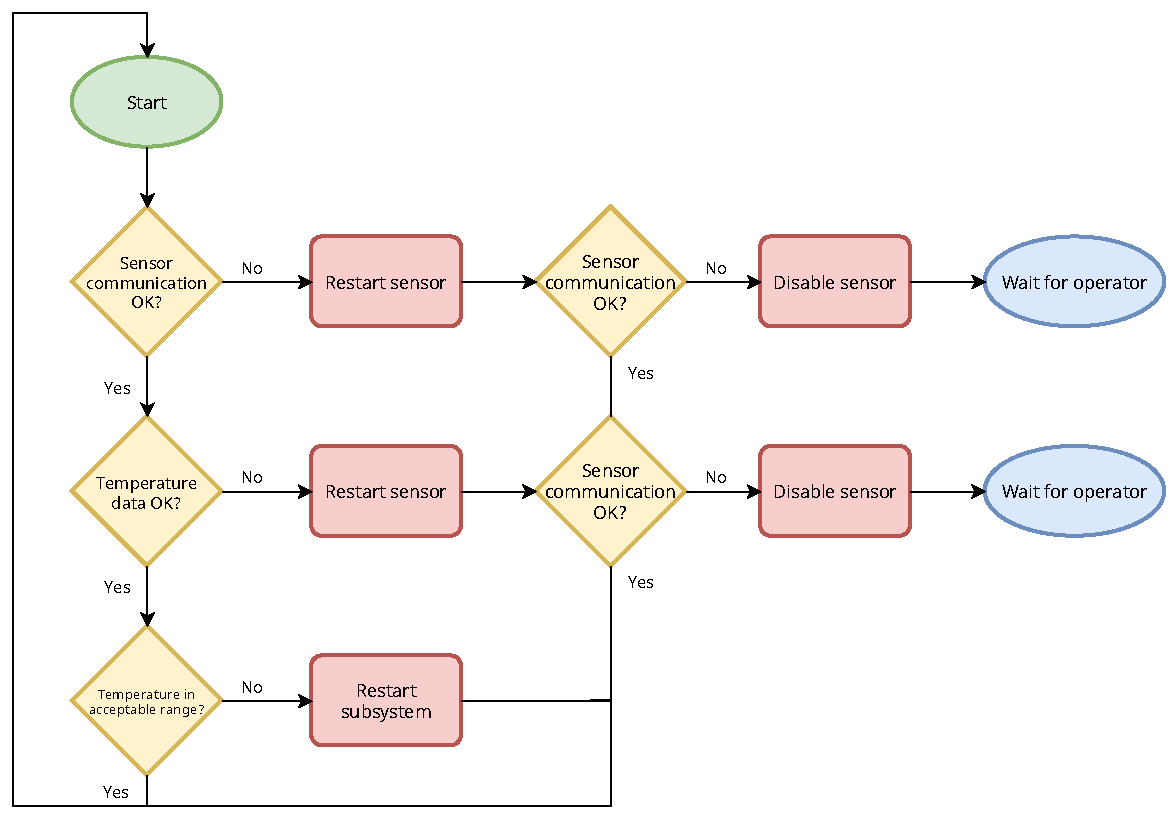
\includegraphics{TempSensorFDIR}
	\caption[Επισκόπηση της διαδικασίας FDIR του αισθητήρα θερμοκρασίας][-3cm]{Σύνοψη της διαδικασίας \ac{FDIR} του αισθητήρα θερμοκρασίας. Για κάθε διεργασία που εκτελείται και για κάθε σφάλμα που εντοπίζεται, παράγεται και η αντίστοιχη τηλεμετρία. \draft{TODO: Μετάφραση}}
	\label{fig:fdirtemp}
\end{figure*}

Το \ac{FDIR} των αισθητήρων ακουλουθεί την ιεραρχική διαδικασία που περιγράφεται στο \Cref{sec:fdir_operating_modes}, που εμφανίζεται στο \Cref{fig:fdirtemp} όπως έχει προσαρμοστεί για τους αισθητήρες.

Η προσέγγιση ακολουθά τα παρακάτω βήματα, τα οποία εκτελούνται διαρκώς στο υπόβαθρο:
\marginnote[2ex]{\g{Για αυτήν την επίδειξη, δεν θα ερευνήσουμε αποτυχίες των εσωτερικών στοιχείων του μικροελεγκτή. Δείτε στο \autocite{retselis_acubesat_fmea_2020} για το πλήρες} \acs{FMEA}\g{ και }\acs{HSIA}\g{ στους μικροελεγκτές.}}


\begin{compactenum}
	\item \g{Παρακολουθείται η κατάσταση υγείας του διαύλου} \ac{I2C} (\Cref{sec:howcani2cfail}). \g{Οποιαδήποτε αποτυχία ή έλλειψη επικοινωνίας υποδεικνύει βλάβη στα ηλεκτρονικά του αισθητήρα.}
	\item \g{Παρακολουθείται η έξοδος θερμοκρασίας των αισθητήρων. Τυχόν τιμές που βρίσκονται εκτός των ορίων των φυσικώς δυνατών θερμικών συνθηκών θεωρούνται ότι υποδηλώνουν βλάβες του αισθητήρα ή της επικοινωνίας. Τυχόν τιμές εκτός των ορίων λειτουργίας των ηλεκτρονικών του υποσυστήματος θεωρούνται ότι υποδηλώνουν υπερθέρμανση και οδηγούν σε επανεκκίνηση του υποσυστήματος.}
	\item \g{Για να διορθωθούν οι αποτυχίες, επιχειρείται πρώτα επανεκκίνηση} (power-cycle) \g{του αισθητήρα. Εάν οι τιμές εξακολουθούν να είναι εσφαλμένες, τότε θεωρείται πως ο αισθητήρας δεν μπορεί να ανακάμψει από την βλάβη, και απλώς απομονώνεται και απενεργοποιείται.}
\end{compactenum}

%\clearpage
\paragraph{\acl{HSIA}}

Αφού έχουμε καθορίσει τους πιθανούς τρόπους αποτυχίας και τη λογική λειτουργίας του συστήματος, είμαστε έτοιμοι να αναλύσουμε κάθε πιθανή αποτυχία για να ορίσουμε τις αναμενόμενες εισόδους λογισμικού για το \ac{FDIR}. Πιο συγκεκριμένα, για κάθε αποτυχία πρέπει να οριστούν τα εξής \autocite[84]{SAVOIR-HB-003}:
\begin{compactitem}
	\item \textbf{Παράμετροι προς παρακολούθηση} για εντοπισμό
	\item \g{\textbf{Εύρη τιμών} για να διαχωρίσουν τις καταστάσεις ύπαρξης ή μη κάποιας αποτυχίας}
	\item \g{Ενέργειες απομόνωσης και ανάκαμψης για την αποτροπή της διάδοσης της αποτυχίας και, εάν είναι δυνατόν, για την επαναφορά του συστήματος σε κανονική λειτουργία.}
\end{compactitem}

Οι παραπάνω πληροφορίες παρατίθενται στον λεγόμενο πίνακα \acf{HSIA}, ο οποίος συνδέει κάθε αποτυχία (που προσδιορίζεται στο \acl{FMEA}) με τις αντίστοιχες παραμέτρους λογισμικού χαμηλού επιπέδου (\cref{tab:hsia}).

Για τους σκοπούς αυτής της επίδειξης, θα θεωρήσουμε ότι όλα τα στοιχεία \ac{FMEA} μπορούν να οδηγήσουν σε \emph{επίφοβες αποτυχίες} (feared events), δηλαδή ότι το \ac{FDIR} θα καλύπτει όλες τις αναγνωρισμένες πιθανές αποτυχίες.

Πιο συγκεκριμένα, το \ac{HSIA} προσθέτει τις ακόλουθες σημαντικές πληροφορίες στο \ac{FMEA} \autocite{ECSS-Q-ST-30-02C}:
\begin{itemize}
	\item \textbf{Παρατηρούμενες παράμετροι} και \textbf{συνθήκες} που πυροδοτούν την ενέργεια ανάκτησης.
	
	\marginnote{\textbf{Προσωρινή αποτυχία}: Προκαλείται από γεγονότα όπως bit flips, θόρυβο ή μεταβατικά φαινόμενα και μπορεί να διορθωθεί χωρίς παρέμβαση ή με μια απλή επανεκκίνηση/κύκλο τροφοδοσίας.\par\textbf{Μόνιμη αποτυχία}: Μια αποτυχία (συνήθως στο υλικό, π.χ. λόγω \acsp{SEL} ή βραχυκυκλωμάτων) που δεν μπορεί να διορθωθεί αυτόνομα.}
	\g{Αυτές παρατίθενται εδώ σε όρους παραμέτρων} \ac{PUS} \g{που μπορούν εύκολα να διαβαστούν και να συγκριθούν από το λογισμικό. Αυτός ο κατάλογος συνδέεται στη συνέχεια με τους αντίστοιχους ορισμούς της υπηρεσίας} \emph{\texttt{ST[12]} on-board monitoring}, \g{που παρατίθενται στον \Cref{tab:demo_monitoring}.}
	
	Είναι σημαντικό να σημειωθεί ότι καμία μεμονωμένη εκτός ορίων τιμή δεν θα πρέπει να προκαλέσει ενέργεια ανάκτησης. Αυτό γίνεται ώστε πρόσκαιρα σφάλματα ή προσωρινά προβλήματα επικοινωνίας να μην μπορούν να οδηγήσουν σε κάποια άσκοπη ενεργοποίηση του \ac{FDIR}, που θα μπορούσε να απενεργοποιήσει ένα καλά λειτουργικό εξάρτημα.
	
	Η διάκριση μεταξύ \emph{προσωρινών} και \emph{μόνιμων} αποτυχιών γίνεται με \textbf{μετρώντας τον αριθμό των διαδοχικών αποτυχιών}. Προτού απενεργοποιηθεί μόνιμα ένας αισθητήρας, πρέπει ενδεικτικά να έχουν αποτύχει τουλάχιστον 5 προσπάθειες επικοινωνίας.
	
	\g{Η χρήση 2 αισθητήρων που λειτουργούν σε ενεργό πλεονασμό επιτρέπει επίσης τη διερεύνηση της διαφοράς μεταξύ των δύο θερμοκρασιών για την εξαγωγή συμπερασμάτων σχετικά με την υγεία των παραγόμενων δεδομένων. Εάν η απόλυτη διαφορά μεταξύ των 2 τιμών είναι πολύ υψηλή, υποθέτοντας ότι οι αισθητήρες βρίσκονται αρκετά κοντά μεταξύ τους, θεωρείται ότι υπάρχει κατάσταση σφάλματος. Ωστόσο, καθώς ο αριθμός των αισθητήρων είναι πολλαπλάσιο του 2, δεν είναι δυνατόν να συμπεράνουμε ποιος αισθητήρας έχει αποτύχει.}
	
	\item \textbf{Δράσεις αποκατάστασης και απομόνωσης βλάβης}.
	
	Αυτές απαριθμούνται σε όρους γεγονότων \ac{PUS} (\emph{\texttt{ST[05]} event reporting}) και ενεργειών (\emph{\texttt{ST[19]} eventaction}), καταγεγραμμένες στον \Cref{tab:demo_eventaction}.
	
	\g{Οι επιλεγμένες ενέργειες αποκατάστασης αντιστοιχούν στην προσέγγιση του \cref{fig:fdirtemp}. Επιπλέον, όταν δεν είναι γνωστό ποιος αισθητήρας έχει αποτύχει, χρησιμοποιείται μια ασφαλής προσέγγιση επανεκκίνησης ή απενεργοποίησης και των δύο αισθητήρων.}
\end{itemize}

\begin{table*}
	\centering
	\caption{Πίνακας HSIA}
	\label{tab:hsia}
	\begin{tabular}{@{}lL{4cm}L{4cm}L{1cm}L{1.1cm}L{3.5cm}@{}}
		\toprule
		ID & Τρόπος Αποτυχίας & Παρατηρούμενες Παράμετροι & ST[12] ID & ST[05] ID & Ενέργεια αποκατάστασης \\ \midrule
		\multicolumn{6}{l}{Αισθητήρας θερμοκρασίας MCP9808 \#1} \\ \midrule
		
		
		
		\textbf{\texttt{F-010}} & Προσωρινή απώλεια λειτουργικότητας & \(\texttt{T1\_Status} = \texttt{TIMEOUT}\) \newline 2 φορές & 0 & 0 & Επανεκκίνηση αισθητήρα 1 \\
		\textbf{\texttt{F-020}} & Μόνιμη απώλεια λειτουργικότητας & \(\texttt{T1\_Status} = \texttt{TIMEOUT}\) \newline 5 φορές & 2 & 2 & Αγνόηση αισθητήρα 1 \\
		\textbf{\texttt{F-030}} & Βραχυκύκλωμα ακροδεκτών ισχύος & \(\texttt{T1\_Status} = \texttt{TIMEOUT}\) \newline 5 φορές & 2 & 2 & Αγνόηση αισθητήρα 1 \\[5ex]
		\textbf{\texttt{F-040}} & Προσωρινή αλλαγή τιμής & 
		\(
		\begin{cases}
			\left|\Delta T\right| & > \SI{20}{\celsius} \text{ ή} \\
			T_1 &> \SI{100}{\celsius} \text{ ή} \\
			T_1 &< \SI{-40}{\celsius}
		\end{cases}
		\) \newline 2 φορές
		 & 4, 6 & 0, 4 & Επανεκκίνηση αισθητήρα 1 \\
		\textbf{\texttt{F-050}} & Μόνιμη αλλαγή τιμής & \(
		\begin{cases}
		\left|\Delta T\right| & > \SI{20}{\celsius} \text{ ή} \\
		T_1 &> \SI{100}{\celsius} \text{ ή} \\
		T_1 &< \SI{-40}{\celsius}
		\end{cases}
		\) \newline 5 φορές & 7, 9 & 2, 5 & Αγνόηση αισθητήρα 1 \\[9ex]
		\textbf{\texttt{F-060}} & Κολλημένος ακροδέκτης εξόδου \acs{I2C} & \(\texttt{T1\_Status} = \texttt{TIMEOUT}\) \newline 5 φορές & 2 & 2 & Αγνόηση αισθητήρα 1 \\ \midrule
		
		
		
		\multicolumn{6}{l}{Αισθητήρας θερμοκρασίας MCP9808 \#2} \\ \midrule
		
		
		
		\textbf{\texttt{F-070}} & Προσωρινή απώλεια λειτουργικότητας & \(\texttt{T2\_Status} = \texttt{TIMEOUT}\) \newline 2 φορές & 1 & 1 & Επανεκκίνησ αισθητήρα 2 \\
		\textbf{\texttt{F-080}} & Μόνιμη απώλεια λειτουργικότητας & \(\texttt{T2\_Status} = \texttt{TIMEOUT}\) \newline 5 φορές & 3 & 3 & Αγνόηση αισθητήρα 2 \\
		\textbf{\texttt{F-090}} & Βραχυκύκλωμα ακροδεκτών ισχύος & \(\texttt{T2\_Status} = \texttt{TIMEOUT}\) \newline 5 φορές & 3 & 3 & Αγνόηση αισθητήρα 2 \\[5ex]
		\textbf{\texttt{F-100}} & Προσωρινή αλλαγή τιμής & 
		\(
		\begin{cases}
		\left|\Delta T\right| & > \SI{20}{\celsius} \text{ ή} \\
		T_2 &> \SI{100}{\celsius} \text{ ή} \\
		T_2 &< \SI{-40}{\celsius}
		\end{cases}
		\) \newline 2 φορές
		& 5, 6 & 1, 4 & Επανεκκίνηση αισθητήρα 2 \\
		\textbf{\texttt{F-110}} & Μόνιμη αλλαγή τιμής & \(
		\begin{cases}
		\left|\Delta T\right| & > \SI{20}{\celsius} \text{ ή} \\
		T_2 &> \SI{100}{\celsius} \text{ ή} \\
		T_2 &< \SI{-40}{\celsius}
		\end{cases}
		\) \newline 5 φορές & 8, 9 & 3, 5 & Αγνόηση αισθητήρα 2 \\[9ex]
		\textbf{\texttt{F-120}} & Κολλημένος ακροδέκτης εξόδου \acs{I2C} & \(\texttt{T2\_Status} = \texttt{TIMEOUT}\) \newline 5 φορές & 3 & 3 & Αγνόηση αισθητήρα 2 \\ \midrule
		
		
		
		\multicolumn{6}{l}{Υποσύστημα} \\ \midrule
		
		
		
		\textbf{\texttt{F-130}} & Υπερθέρμανση & \(T_1 > \SI{40}{\celsius}\) or \(T_2 > \SI{40}{\celsius}\) & 10, 11 & 6 & Επανεκκίνηση υποσυστήματος \\ \bottomrule
	\end{tabular}
	\vspace{2pt}
\end{table*}

%\clearpage

\paragraph{Παράμετροι}

Μετά την ολοκλήρωση της \acl{HSIA}, είμαστε έτοιμοι να ορίσουμε τις αριθμητικές παραμέτρους της υπηρεσίας \emph{\texttt{ST[20]} on-board parameter management} \autocite{ECSS-E-ST-70-41C} (\cref{tab:demo_params}).

Πέρα από τις εξόδους των αισθητήρων, έχουμε συμπεριλάβει τη \textbf{διαφορά} (\(\Delta\)) μεταξύ των δύο θερμοκρασιών, καθώς το πρότυπο \acs{PUS} δεν παρέχει τρόπους για την εκτέλεση αριθμητικών υπολογισμών. Επιπλέον, περιλαμβάνεται η κατάσταση λειτουργίας του κάθε αισθητήρα, η οποία είναι μια απαριθμημένη (enumerated) τιμή.\footnote{Η τιμή μπορεί να είναι μία από τις \texttt{NOMINAL} (ο αισθητήρας λειτουργεί κανονικά), \texttt{TIMEOUT} (έχει εντοπιστεί κάποιο σφάλμα) ή \texttt{DISABLED} (ο αισθητήρας είναι ρητά απενεργοποιημένος)} 

Αυτές οι παράμετροι τηλεμετρώνται στον σταθμό βάσης και εμφανίζονται στο χρήστη περιοδικά, μέσω της υπηρεσίας \emph{\texttt{ST[03]} housekeeping} \ac{PUS} και των ραδιοφάρων που αυτή εκπέμπτη. Ωστόσο, όταν το CubeSat βρίσκεται στο διάστημα, ο σταθμός βάσης δεν θα έχει συνεχή πρόσβαση σε αυτά τα δεδομένα, καθώς ο δορυφόρος δεν θα είναι ορατός από τους επίγειους σταθμούς καθ' όλη τη διάρκεια της τροχιάς του.

\begin{table}[h]
	\centering
	\caption[Λίστα παραμέτρων \texttt{ST[20]}]{\g{Λίστα παραμέτρων} \texttt{ST[20]}\\R: Μόνο ανάγνωση\\RW: Ανάγνωση και εγγραφή}
	\label{tab:demo_params}
	\begin{tabularx}{\textwidth}{@{}rXlll@{}}
		\toprule
		ID & Παράμετρος              & Μονάδα & Τύπος & Εγγραφή \\ \midrule
		0            & Θερμοκρασία 1          & \si{\celsius}      & \texttt{float} & R     \\
		1            & Θερμοκρασία 2          & \si{\celsius}      & \texttt{float} & R    \\
		2            & \(\Delta\) Θερμοκρασίας & \si{\celsius}      & \texttt{float} & R    \\
		3            & Κατάσταση Θερμοκρασία 1         &       & Απαρίθμηση   & RW  \\
		4            & Κατάσταση Θερμοκρασία 2         &       & Απαρίθμηση   & RW  \\
		5			 & Κατάσταση Θερμοκρασία 1+2       &		& Απαρίθμηση   & R  \\ \bottomrule
	\end{tabularx}
\end{table}

\paragraph{Ορισμοί παρακολούθησης}

Μετά τον ορισμό των παραμέτρων, θα πρέπει να περιγραφούν οι ορισμοί παρακολούθησης που καθορίζουν τα αποδεκτά και μη εύρη τιμών για κάθε παράμετρο. Η διαχείριση αυτών γίνεται από την υπηρεσία \emph{\texttt{ST[12]} on-board monitoring} του \ac{PUS}.

\g{Οι \emph{συνθήκες εγκυρότητας ελέγχου} είναι σημαντικό να αναφερθούν σε αυτή την περίπτωση, καθώς χρησιμοποιούν τις τρεις παραμέτρους \emph{Κατάστασης} του \Cref{tab:demo_params} για να αποτρέψουν την εκτέλεση ελέγχων σε απενεργοποιημένα περιφερειακά.} \g{Ως εκ τούτου, οι αισθητήρες που δεν παρέχουν τιμές λόγω προβλημάτων υλικού, ενεργειών} \ac{FDIR} ή κάποιας ρητής τηλεεντολής από το Σταθμό Βάσης, δεν θα μπορούν να ενεργοποιήσουν ενέργειες \ac{FDIR}.

\begin{table*}[h]
	\centering
	\caption[Λίστα ορισμών παρακολούθησης της υπηρεσίας \texttt{ST[12]}][5pt]{Λίστα ορισμών παρακολούθησης της υπηρεσίας \texttt{ST[12]}. Τα σύμβολα \(t\) και \(\Delta\) αναπαριστούν τις εκάστοτε τιμές των παραμέτρων.}
	\label{tab:demo_monitoring}
	\begin{adjustbox}{width=\textwidth}
	\begin{tabular}{@{}L{1cm}L{3.2cm}L{3.6cm}L{1.5cm}L{1.5cm}L{1.2cm}ll@{}}
		\toprule
		&  & \multicolumn{2}{c}{Συνθήκες εγκυρότητας ελέγχου} &  &  & \multicolumn{2}{c}{Έλεγχος} \\ \cmidrule(lr){3-4} \cmidrule(l){7-8} 
		ID & Παρακολουθούμενη παράμετρος & Παράμετρος εγκυρότητας & Αναμενόμενη τιμή & Περίοδος & Αρ. μετρήσεων & Είδος & Κριτήριο \\ \midrule
		0 & Κατάσταση Θερμ. 1 &  &  & \SI{500}{\milli\second} & 2 & Ισότητα & \(\neq\) \texttt{TIMEOUT} \\
		1 & Κατάσταση Θερμ. 2 &  &  & \SI{500}{\milli\second} & 2 & Ισότητα & \(\neq\) \texttt{TIMEOUT} \\
		2 & Κατάσταση Θερμ. 1 &  &  & \SI{500}{\milli\second} & 5 & Ισότητα & \(\neq\) \texttt{TIMEOUT} \\
		3 & Κατάσταση Θερμ. 2 &  &  & \SI{500}{\milli\second} & 5 & Ισότητα & \(\neq\) \texttt{TIMEOUT} \\
		\midrule
		4 & Θερμοκρασία 1 & Κατάσταση Θερμ. 1 & \texttt{NOMINAL} & \SI{500}{\milli\second} & 2 & Εύρος & \( -\SI{40}{\celsius} < t < \SI{100}{\celsius} \) \\
		5 & Θερμοκρασία 2 & Κατάσταση Θερμ. 2 & \texttt{NOMINAL} & \SI{500}{\milli\second} & 2 & Εύρος & \( -\SI{40}{\celsius} < t < \SI{100}{\celsius} \) \\
		6 & \(\Delta\) Θερμοκρασία & Κατάσταση Θερμ. 1+2 & \texttt{NOMINAL} & \SI{500}{\milli\second} & 2 & Εύρος & \( -\SI{20}{\celsius} < \Delta < \SI{20}{\celsius} \) \\
		\midrule
		7 & Θερμοκρασία 1 & Κατάσταση Θερμ. 1 & \texttt{NOMINAL} & \SI{500}{\milli\second} & 5 & Εύρος & \( -\SI{40}{\celsius} < t < \SI{100}{\celsius} \) \\
		8 & Θερμοκρασία 2 & Κατάσταση Θερμ. 2 & \texttt{NOMINAL} & \SI{500}{\milli\second} & 5 & Εύρος & \( -\SI{40}{\celsius} < t < \SI{100}{\celsius} \) \\
		9 & \(\Delta\) Θερμοκρασία & Κατάσταση Θερμ. 1+2 & \texttt{NOMINAL} & \SI{500}{\milli\second} & 5 & Εύρος & \( -\SI{20}{\celsius} < \Delta < \SI{20}{\celsius} \) \\
		\midrule
		10 & Θερμοκρασία 1 & Κατάσταση Θερμ. 1 & \texttt{NOMINAL} & \SI{500}{\milli\second} & 5 & Εύρος & \( t < \SI{50}{\celsius} \) \\
		11 & Θερμοκρασία 2 & Κατάσταση Θερμ. 2 & \texttt{NOMINAL} & \SI{500}{\milli\second} & 5 & Εύρος & \( t < \SI{50}{\celsius} \) \\ \bottomrule
	\end{tabular}
	\end{adjustbox}
\end{table*}
\vspace{2ex}
\FloatBarrier

\paragraph{Event-action definitions}

Το τελευταίο κομμάτι του παζλ είναι οι ορισμοί των γεγονότων-αντιδράσεων (event-actions), που μπορούν να φανούν στον \Cref{tab:demo_eventaction} και συνδυάζουν:
\begin{itemize}
	\item \ac{PUS} γεγονότα (υπηρεσία \texttt{ST[05]}), τα οποία εκπέμπονται αυτόματα όταν ένας ορισμός παρακολούθησης ξεπερνά τα όριά του
	\item \ac{PUS} ορισμοί γεγονότων-αντιδράσεων (υπηρεσία \texttt{ST[19]}), \g{οι οποίοι συνδέουν κάθε εμφάνιση ενός γεγονότος με μία αποθηκευμένη τηλεεντολή που εκτελείται αμέσως και αναπαριστά τις διαδικασίες ανάκτησης του} \acs{FDIR}.
\end{itemize}

Όλοι αυτοί οι ορισμοί μπορούν εύκολα να τροποποιηθούν από τους χειριστές με τη χρήση μεμονωμένων τηλεεντολών, οι οποίες επιδρούν επάνω στην βάση δεδομένων του διαστημικού εξοπλισμού.

\begin{table}[h]
	\centering
	\caption{Λίστα ορισμών γεγονότων-αντιδράσεων της υπηρεσίας \texttt{ST[19]}}
	\label{tab:demo_eventaction}
	\begin{tabularx}{\textwidth}{@{}L{1.8cm}L{2cm}X@{}}
		\toprule
		ID γεγονότος & Ορισμός Παρακολούθησης & Αντίδραση \\ \midrule
		0 & 0, 4 & Επανεκκίνηση αισθητήρα 1 \\
		1 & 1, 5 & Επανεκκίνηση αισθητήρα 2 \\
		2 & 2, 7 & Κατάσταση αισθητήρα 1 \( = \) \texttt{DISABLED} \\
		3 & 3, 8 & Κατάσταση αισθητήρα 2 \( = \) \texttt{DISABLED} \\
		4 & 6 & Επανεκκίνηση αισθητήρων 1 + 2 \\
		5 & 9 & Κατάσταση αισθητήρων 1 + 2 \( = \) \texttt{DISABLED} \\
		6 & 10, 11 & Επανεκκίνηση συστήματος \\ \bottomrule
	\end{tabularx}
\end{table}

\clearpage
\section{Επικύρωση \acs{FDIR}}

\subsection{Κανονική λειτουργία}

Στην κανονική λειτουργία, δεν προσομοιώνεται καμία βλάβη. Το σύστημα είναι ενεργοποιημένο και παράγει τηλεμετρία που υπακούει στα πρότυπα \ac{ECSS} (\Cref{fig:yamcshousekeeping}), η οποία περιλαμβάνει τιμές παραμέτρων που αναλύονται από το \acs{YAMCS} (\Cref{fig:yamcsparameter}). Επιπλέον, διατηρείται ένα αρχείο καταγραφής για διαγνωστικούς σκοπούς (\Cref{fig:lognominal}). Το σύστημα συμμορφώνεται με τις ορισμένες απαιτήσεις (\Cref{sec:tsvcd}) και μπορεί να μεταδώσει τη θερμοκρασία στον Σταθμο Βάσης, όπως είναι αναμενόμενο.

\begin{figure}
	\centering
	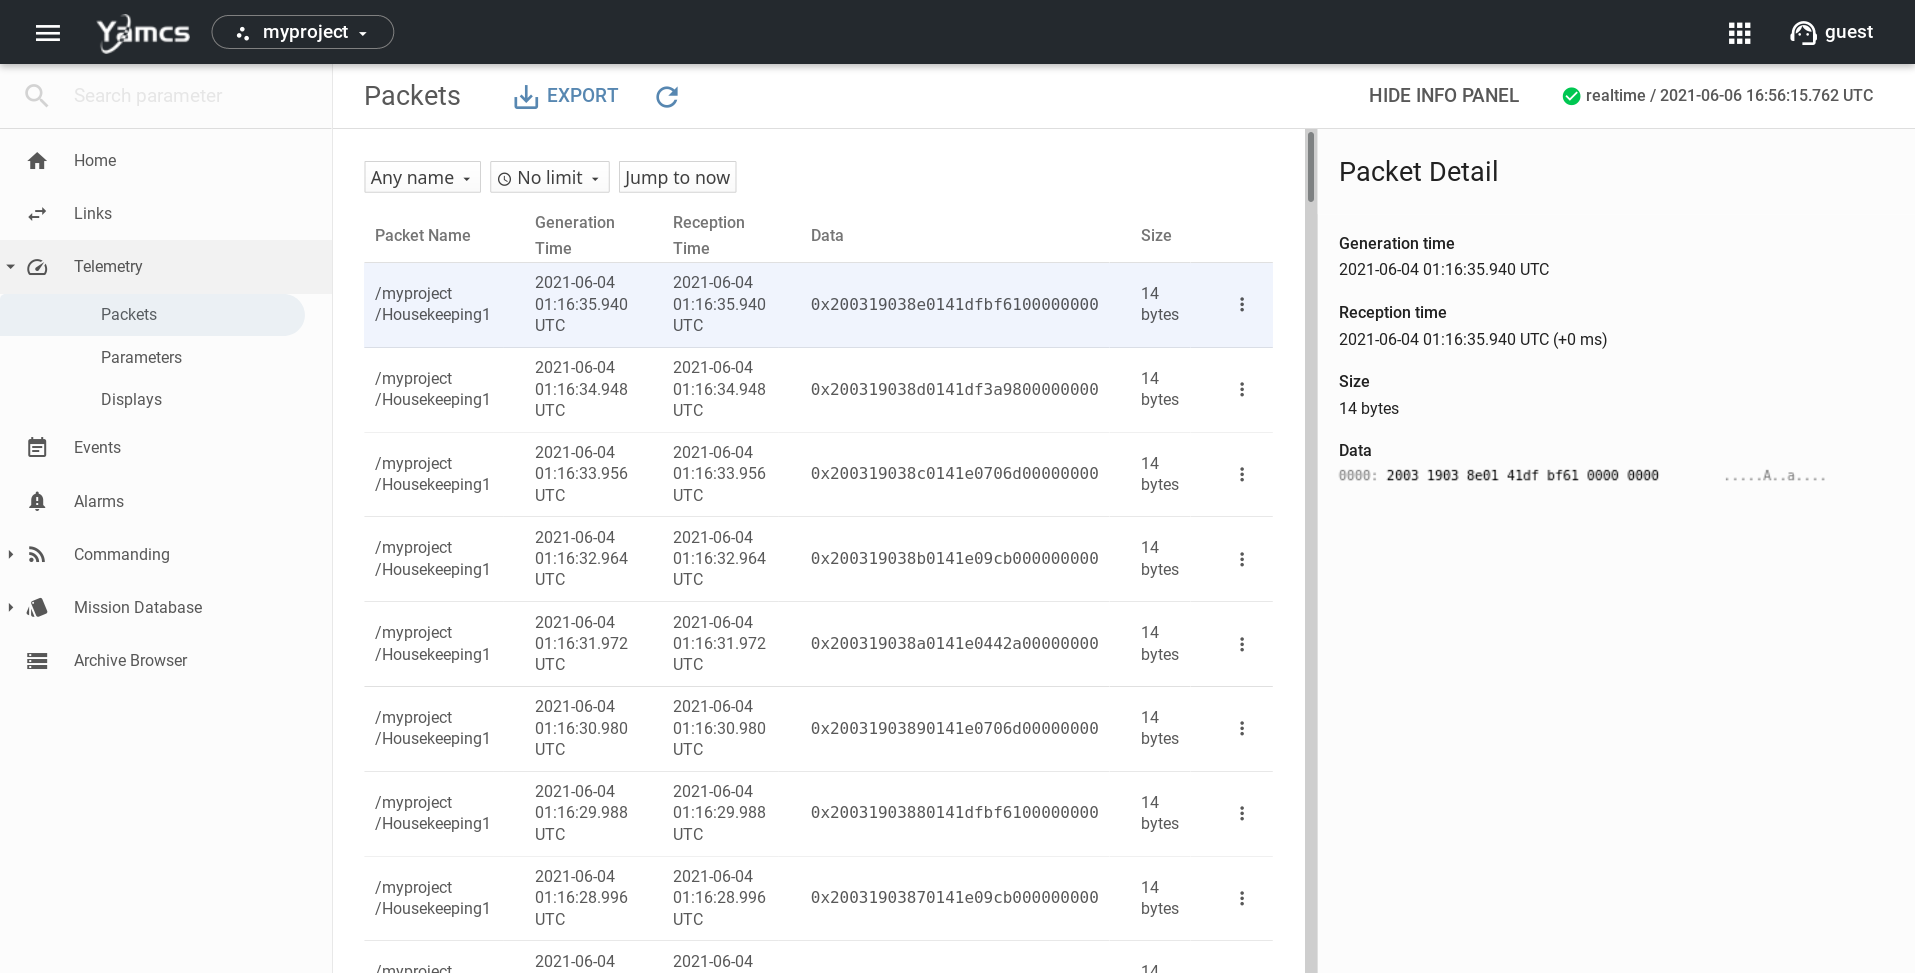
\includegraphics{media/screenshots/yamcs_housekeeping}
	\caption{Περιοδικοί ραδιοφάροι που παράγονται από τον μικροελεγκτή, όπως φαίνονται στο \acs{YAMCS}}
	\label{fig:yamcshousekeeping}
\end{figure}

\begin{figure}[h]
	\centering
	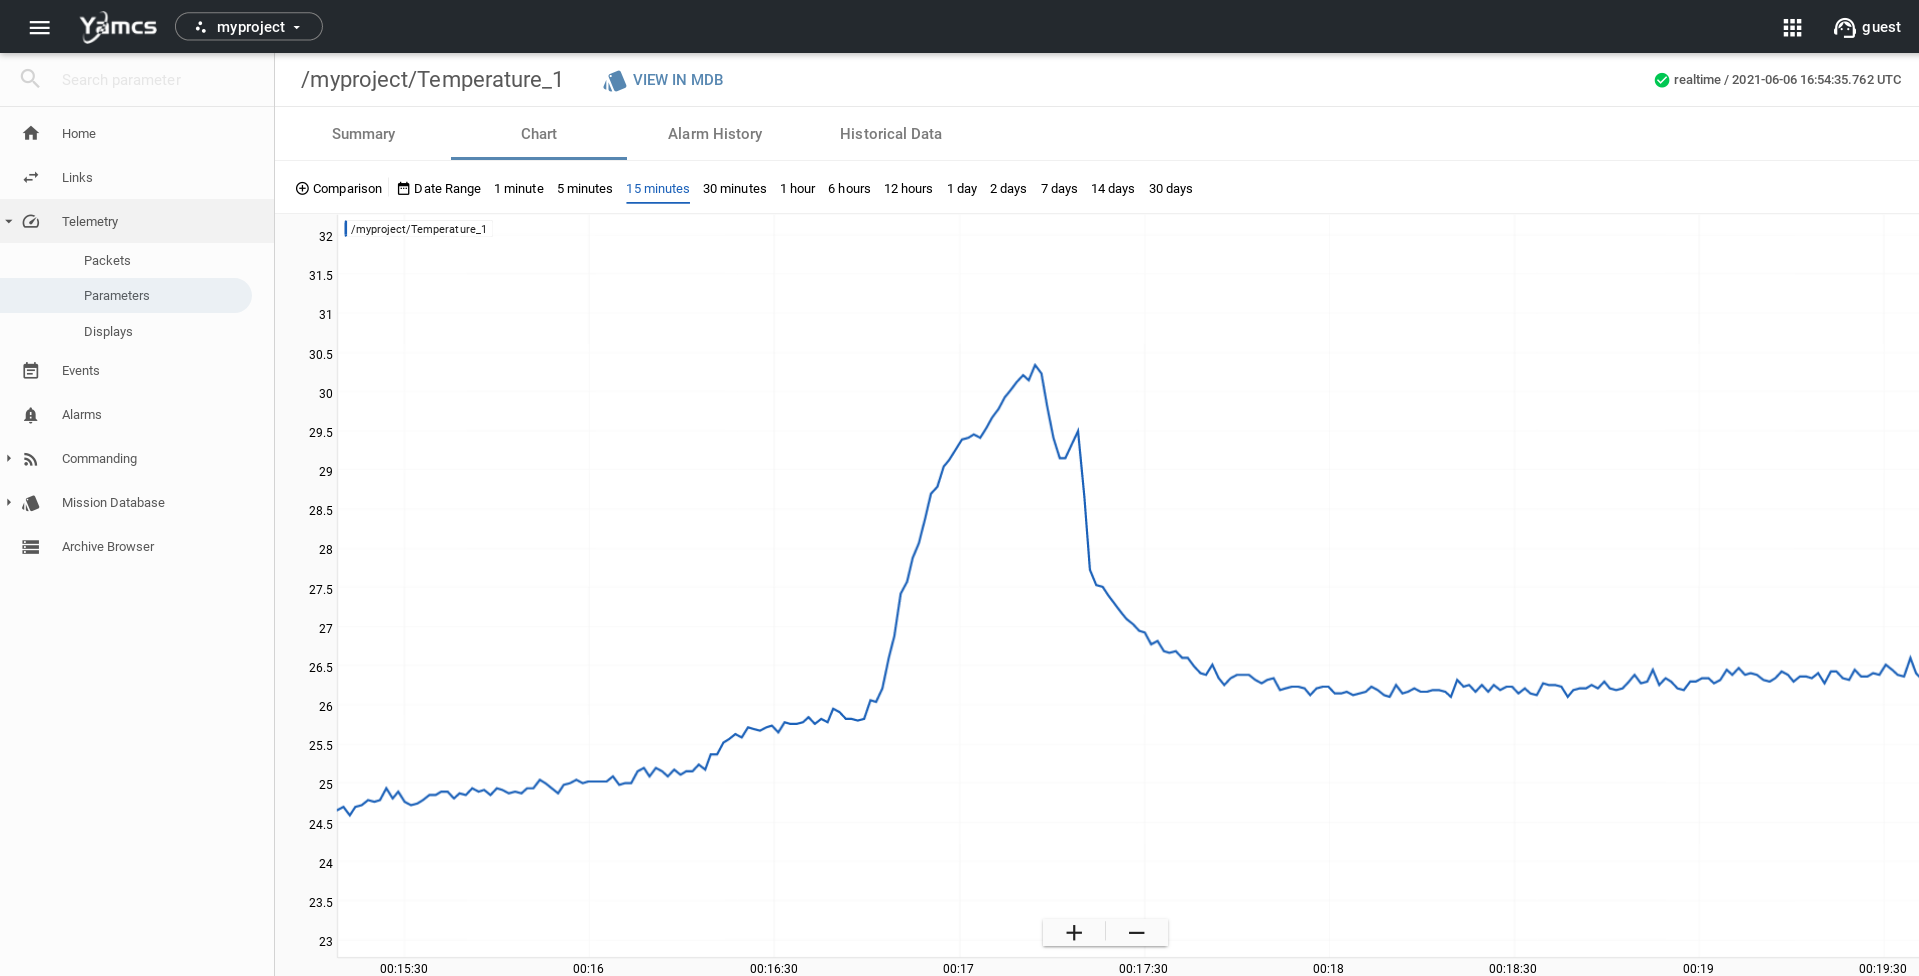
\includegraphics{media/screenshots/yamcs_parameter}
	\caption{Εξέλιξη μιας παραμέτρου θερμοκρασίας στο χρόνο, όπως φαίνεται στο \acs{YAMCS}}
	\label{fig:yamcsparameter}
\end{figure}

\begin{figure}
\begin{cminted}{text}
909601  [debug  ] T1 = 28.18
909701  [debug  ] T1 = 28.08
909801  [debug  ] T1 = 28.14
909901  [debug  ] T1 = 27.97
910000  [trace  ] New TM [3,25]
910001  [debug  ] T1 = 28.10
910101  [debug  ] T1 = 28.03
910201  [debug  ] T1 = 28.12
910301  [debug  ] T1 = 27.90
910401  [debug  ] T1 = 28.08
\end{cminted}
\caption[Έξοδος καταγραφής σε κανονική λειτουργία]{Έξοδος καταγραφής σε κανονική λειτουργία. Ο πρώτος αριθμός δηλώνει τους χτύπους ρολογιού του μικροελεγκτή, που μετρώνται σε χιλιοστά του δευτερολέπτου από την εκκίνηση.}
\label{fig:lognominal}
\end{figure}

\marginnote{Γενικά είδη κατάστασης \autocite{ECSS-E-ST-70-41C}:
	
	\texttt{Unchecked}: Ο έλεγχος είναι απενεργοποιημένος.
	
	\texttt{OK}: Η μεταβλητή βρίσκεται εντός ορίων.
	
	\texttt{Invalid}: Η συνθήκη εγκυρότητας του ελέγχου είναι ψευδής. Ο έλεγχος δεν πραγματοποιείται.
}

Ιδιαίτερο ενδιαφέρον έχει να παρατηρήσουμε την κατάσταση του συστήματος \acs{FDIR} κατά την εκκίνηση. Η πρώτη πληροφορία που λαμβάνουμε φαίνεται στην \Cref{fig:pus_boot}. Η εικόνα αυτή δείχνει τις \textbf{μεταβάσεις (transitions)} της υπηρεσίας \emph{\texttt{ST[12]} on-board monitoring}, όπως φαίνονται στην διεπαφή που αναπτύξαμε (\Cref{sec:pusinterface}). Πρακτικά, αυτή η προβολή δείχνει το \textbf{αποτέλεσμα} του κάθε ελέγχου, και αν η τιμή είναι εντός ορίων, εκτός ορίων, ή αν ο έλεγχος είναι απενεργοποιημένος.

\begin{figure}
	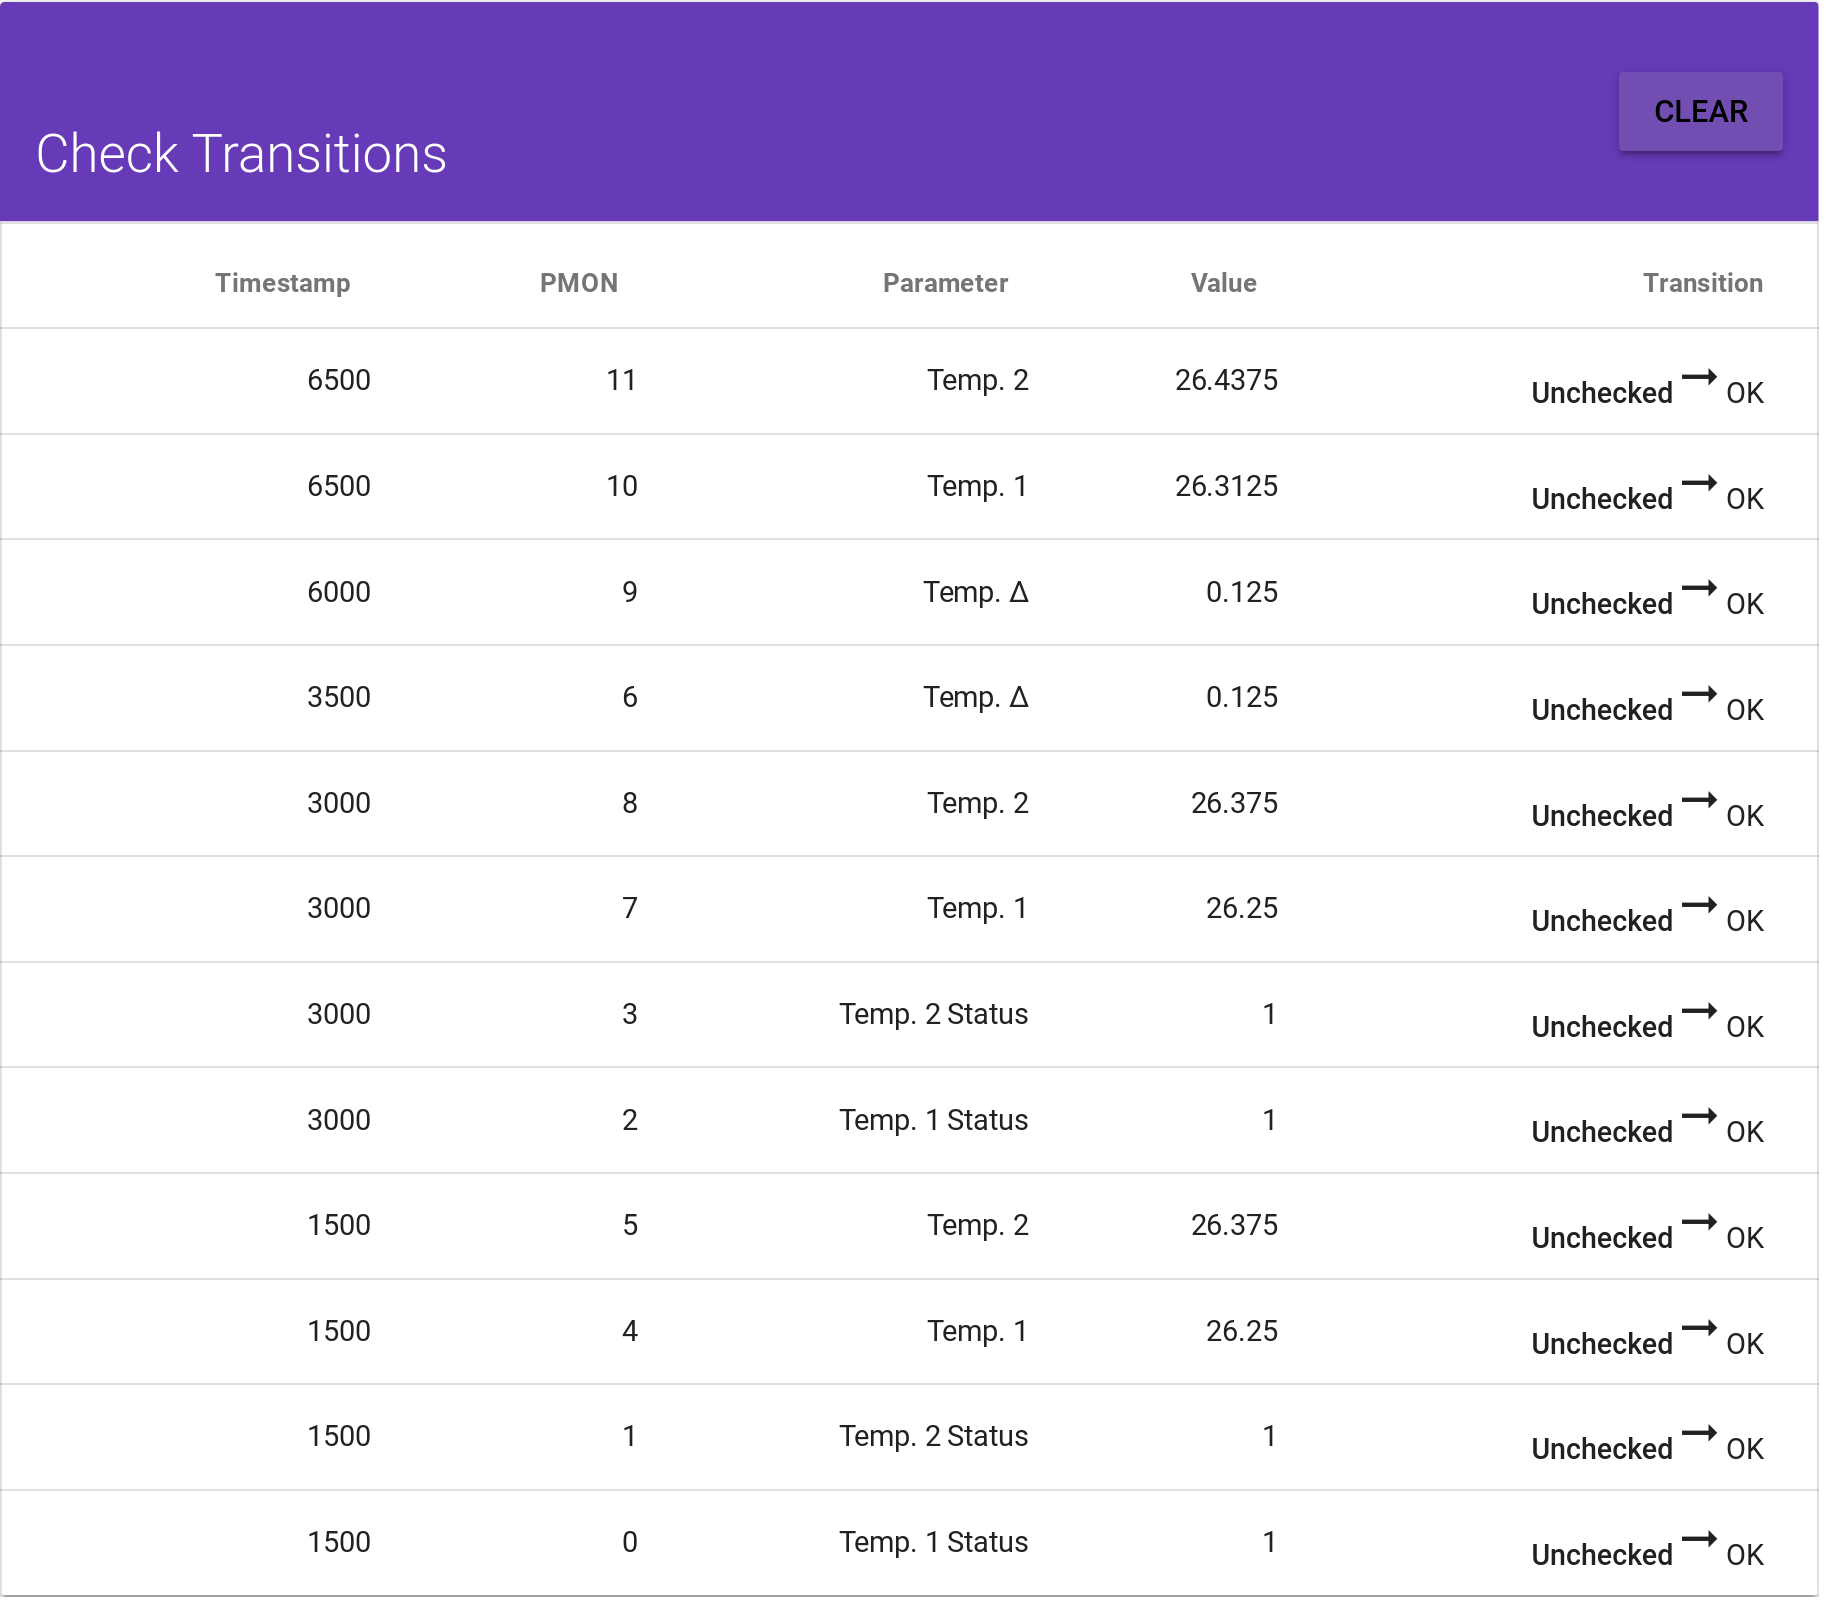
\includegraphics{screenshots/pus_boot}
	\caption{Μεταβάσεις που πραγματοποιούνται κατά την εκκίνηση}
	\label{fig:pus_boot}
\end{figure}

Στο συγκεκριμένο παράδειγμα, παρατηρούμε ότι και οι 12 \g{καταχωρημένοι} έλεγχοι μεταβαίνουν από την κατάσταση \texttt{Unchecked} στην κατάσταση \texttt{OK}. Αυτό συμβαίνει καθώς, με την εκκίνηση του συστήματος, όλοι οι ορισμοί παρακολούθησης βρίσκονται στην αρχική κατάσταση \texttt{Unchecked}, που δηλώνει πως δεν έχουν πραγματοποιηθεί ποτέ. Μετά από την πάροδο της περιόδου μετρήσεων \emph{επί} του αριθμού επαναλήψεων του κάθε ορισμού, η μεταβλητή θεωρείται πως έχει τιμή εντός ορίων, και ο ορισμός είναι \texttt{OK}.

Ο διαφορετικός χρόνος μετάβασης του κάθε ορισμού οφείλεται στον διαφορετικό \textbf{αριθμό επαναλήψεων}. Για να καταχωρηθεί η μετάβαση, πρέπει η μεταβλητή να έχει μετρηθεί όσες φορές δηλώνει αυτός ο αριθμός, που ορίζεται από τους χειριστές.

Εφ' όσον οι μεταβάσεις οδηγούν σε μια κατάσταση εντός ορίων, δεν παράγεται κάποια άλλη αναφορά, ούτε πυροδοτείται κάποιος άλλος μηχανισμός επιδιόρθωσης. Το σύστημα λειτουργεί σωστά.

\begin{figure}[h]
	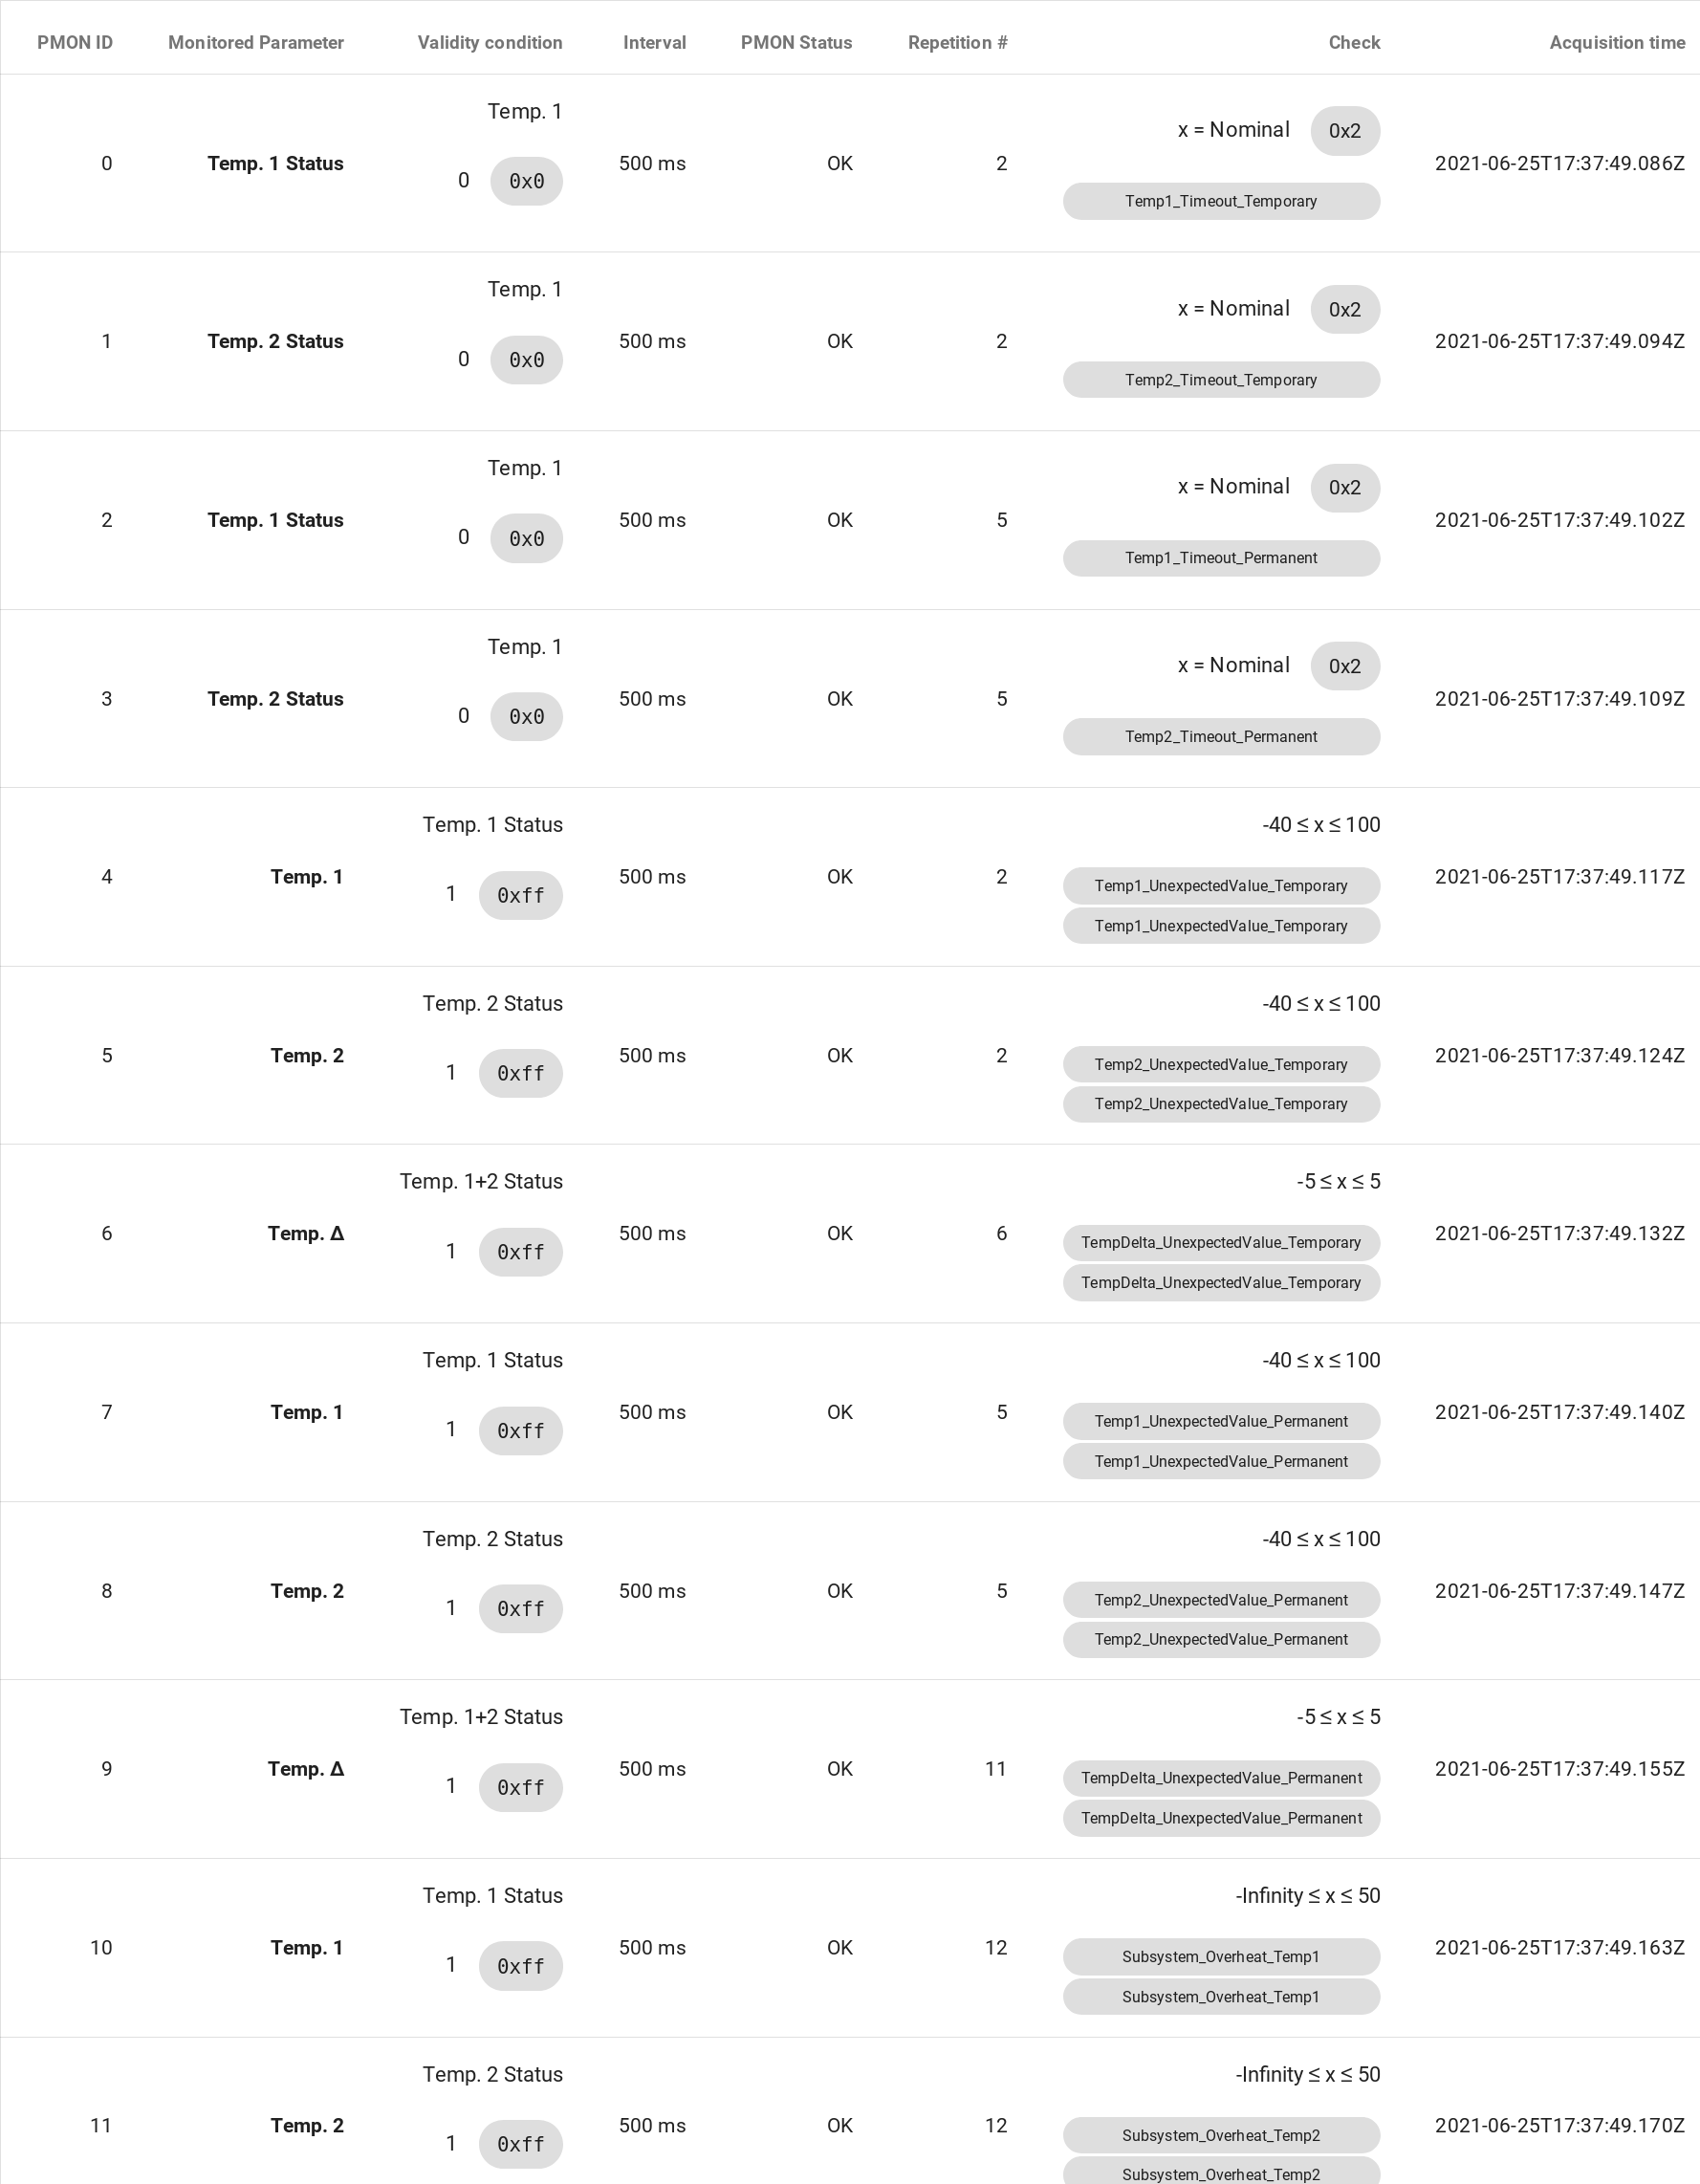
\includegraphics{screenshots/pus_obmd}
	\caption[Λίστα ορισμών παρακολούθησης στην εκκίνηση, χωρίς καμία αποτυχία]{Λίστα ορισμών παρακολούθησης στην εκκίνηση, χωρίς καμία αποτυχία. Τα δεδομένα αυτά λαμβάνονται ως τηλεμετρία από τον μικροελεγκτή και αντιστοιχούν ακριβώς στις τιμές του \Cref{tab:demo_monitoring}.}
	\label{fig:pus_obmd}
\end{figure}

\begin{figure}[h]
	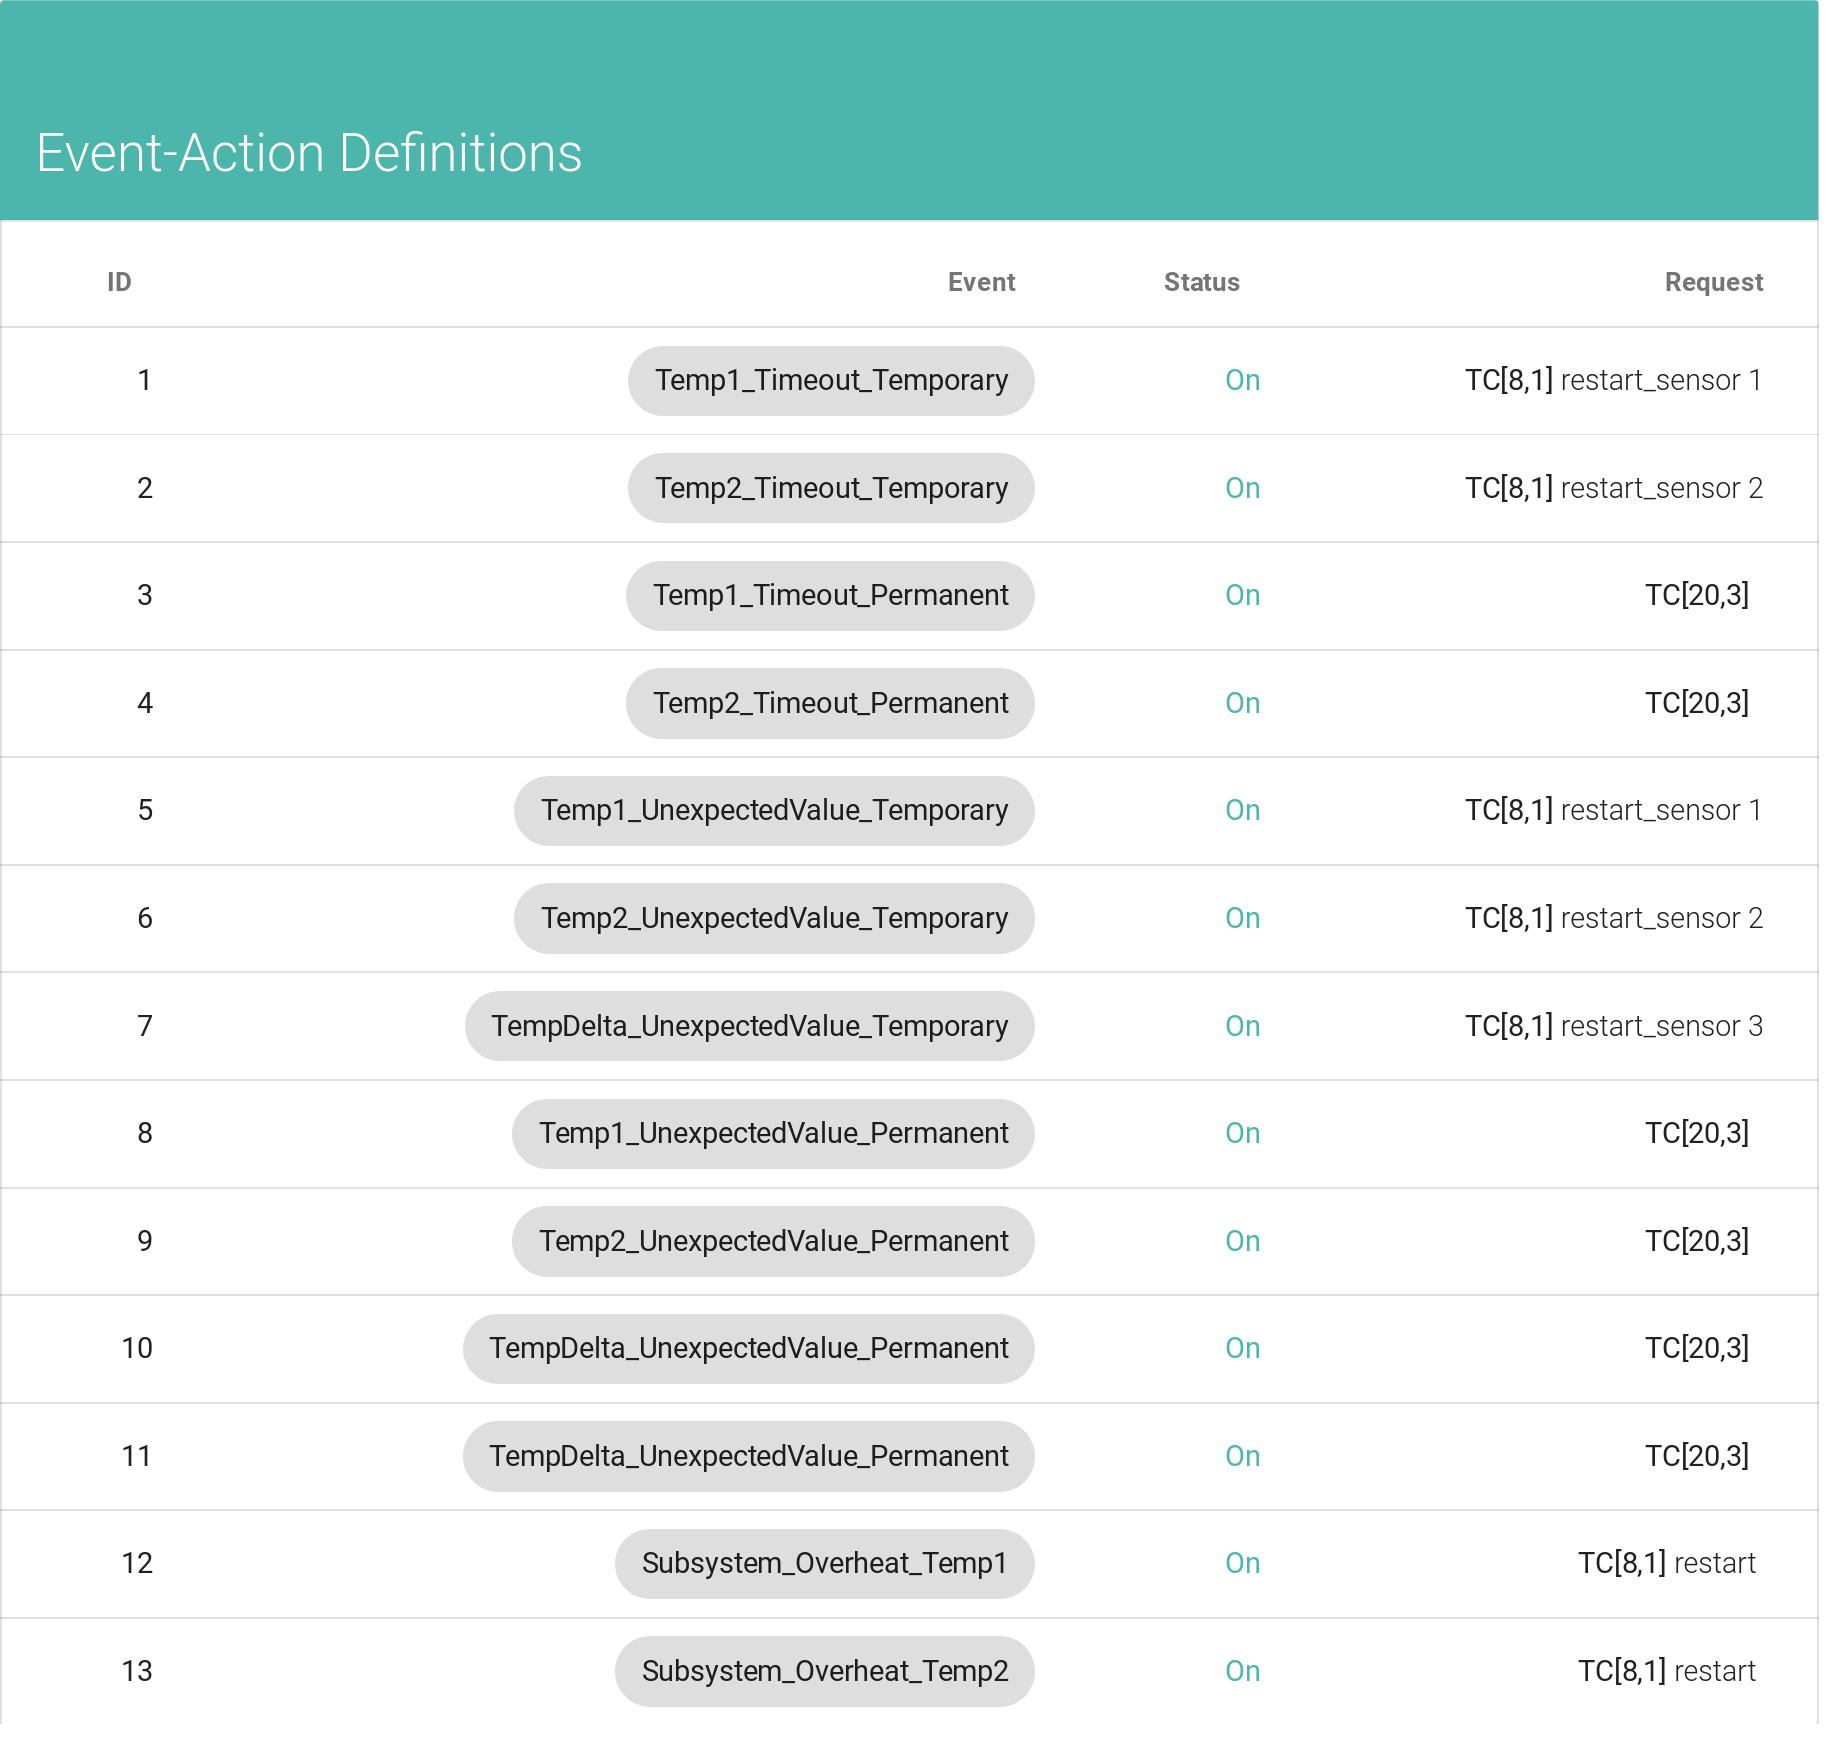
\includegraphics{screenshots/pus_eventaction}
	\caption[Λίστα ορισμών γεγονότος-αντίδρασης]{Λίστα ορισμών γεγονότος-αντίδρασης στην εκκίνηση, χωρίς καμία αποτυχία. Τα δεδομένα αυτά λαμβάνονται ως τηλεμετρία από τον μικροελεγκτή και αντιστοιχούν ακριβώς στις τιμές του \Cref{tab:demo_eventaction}.}
	\label{fig:pus_eventaction}
\end{figure}

\g{Ακόμα, κατά την εκκίνηση, δημιουργείται ένα \textbf{γεγονός} της υπηρεσίας} \emph{\texttt{ST[05]} event reporting} \g{που ανακοινώνει την εκκίνηση του μικροελεγκτή} (\Cref{fig:yamcsmcustart}).

\begin{figure}[h]
	\centering
	\caption{Το γεγονός έναρξης του μικροελεγκτή, μέσα από το \acs{YAMCS}}
	\label{fig:yamcsmcustart}
	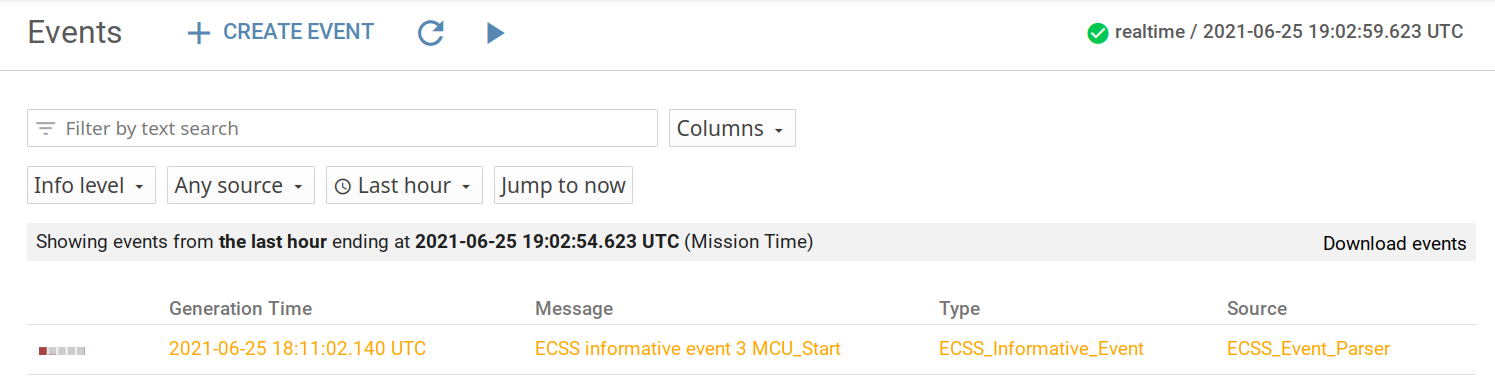
\includegraphics{screenshots/yamcs_mcustart}
\end{figure}

\FloatBarrier
\subsection{Προσομοίωση αστοχιών}
\label{sec:simul}

\selectlanguage{greek}
Για την προσομοίωση κάθε αποτυχίας χρησιμοποιήθηκαν οι ακόλουθες μέθοδοι:
\begin{itemize}
	\item Για τις αποτυχίες επικοινωνίας μεταξύ εξαρτημάτων, κάθε αισθητήρας απλά αποσυνδέθηκε φυσικά από το σύστημα.
	\item Για μικρές αλλαγές στη θερμοκρασία, ένα πιστόλι θερμού αέρα ή άλλη πηγή θερμότητας στρεφόταν προς κάθε αισθητήρα, με κατάλληλη φροντίδα ώστε να μη ξεπεραστούν τα λειτουργικά όρια των εξαρτημάτων.
	\item Για μεταβολές της θερμοκρασίας που δεν ήταν πρακτικά δυνατό να προσομοιωθούν, η βλάβη εισήχθη στο λογισμικό, τροποποιώντας χειροκίνητα τις αντίστοιχες μεταβλητές.
	
	Τα δύο κουμπιά που υπάρχουν στην αναπτυξιακή πλακέτα χρησιμοποιήθηκαν ένα απλό μέσο για την "εισαγωγή" ακραίων τιμών θερμοκρασίας.
\end{itemize}
\selectlanguage{english}

\begin{table*}
	\centering
	\caption{Σύνοψη μεθόδων δοκιμής αποτυχιών}
	\label{tab:testfailures}
	\renewcommand{\arraystretch}{1.5}
	\begin{tabularx}{\textwidth}{@{}lL{4cm}L{3.5cm}X@{}}
		\toprule
		ID & Τρόπος Αποτυχίας & Ενέργεια αποκατάστασης & Τρόπος προσομοίωσης \\ \midrule
		\multicolumn{4}{l}{Αισθητήρας θερμοκρασίας MCP9808 \#1} \\ \midrule
		\textbf{\texttt{F-010}} & Προσωρινή απώλεια λειτουργικότητας & Επανεκκίνηση αισθητήρα 1 & \textbf{Υλικό}: Προσωρινή αποσύνδεση καλωδίου \\
		\textbf{\texttt{F-020}} & Μόνιμη απώλεια λειτουργικότητας & Αγνόηση αισθητήρα 1 & \textbf{Υλικό}: Μόνιμη αποσύνδεση καλωδίου \\
		\textbf{\texttt{F-030}} & Βραχυκύκλωμα ακροδεκτών ισχύος & Αγνόηση αισθητήρα 1 & \emph{Ίδιο με \texttt{F-020}}  \\
		\textbf{\texttt{F-040}} & Προσωρινή αλλαγή τιμής & Επανεκκίνηση αισθητήρα 1 & \textbf{Λογισμικό}: Προσομοίωση μεγάλης τιμής (προσωρινά)\newline \textbf{Υλικό}: Αύξηση θερμοκρασιακής διαφοράς (προσωρινά)\\
		\textbf{\texttt{F-050}} & Μόνιμη αλλαγή τιμής & Αγνόηση αισθητήρα 1 & \textbf{Λογισμικό}: Προσομοίωση μεγάλης τιμής (μόνιμα)\newline\textbf{Υλικό}: Αύξηση θερμοκρασιακής διαφοράς (μόνιμα) \\
		\textbf{\texttt{F-060}} & Κολλημένος ακροδέκτης εξόδου \acs{I2C} & Αγνόηση αισθητήρα 1 & \textbf{Υλικό}: Σύνδεση ακροδέκτη στη γείωση
		\\ \midrule
		\multicolumn{4}{l}{Αισθητήρας θερμοκρασίας MCP9808 \#2} \\ \midrule
		
		\multicolumn{4}{@{}c@{}}{Ίδιο με τον αισθητήρα \#1\vspace{1ex}} \\ \midrule
		
		\multicolumn{4}{l}{Υποσύστημα} \\ \midrule
		
		
		\textbf{\texttt{F-130}} & Υπερθέρμανση  & Επανεκκίνηση υποσυστήματος & \textbf{Υλικό}: Αύξηση θερμοκρασίας αισθητήρα \\ \bottomrule
	\end{tabularx}
	\vspace{2pt}
\end{table*}

\FloatBarrier

\paragraph{\textbf{\texttt{F-010}: Προσωρινή απώλεια λειτουργικότητας}}~

Η πρώτη αποτυχία που θα προσομοιώσουμε θα είναι η απώλεια λειτουργίας του διαύλου \acs{I2C} ή του περιφερειακού. Η προσομοίωση γίνεται στο υλικό μέσω της \emph{προσωρινής αποσύνδεσης καλωδίου}.

\subparagraph{Διαδικασία} \draft{διόρθωση εσοχής}
\begin{compactenum}
	\item Αποσυνδέουμε το καλώδιο \acs{SDA} ή \acs{SCL} από το breadboard
	\item \g{Μετά από 2 δευτερόλεπτα, επανασυνδέουμε το καλώδιο, ώστε να αναπαραστήσουμε μία προσωρινή (και όχι μόνιμη) βλάβη}
\end{compactenum}

\subparagraph{Οπτική ένδειξη} Η 1\textsuperscript{η} ενδεικτική λυχνία αναβοσβήνει μία φορά, και παραμένει ανοιχτή.

\subparagraph{Αποτελέσματα}
Για αυτήν την αποτυχία, θα παρουσιαστούν με λεπτομέρεια όλες οι διαδικασίες που συμβαίνουν στο υπόβαθρο και πώς φαίνονται σε έναν χειριστή. Στις επόμενες αναλύσεις, τα αποτελέσματα αυτά θα παρουσιαστούν μόνο συνοπτικά, χρησιμοποιώντας το εργαλείο του πίνακα μεταβάσεων.

Προτού μελετήσουμε τα αποτελέσματα της αποτυχίας και του \acs{FDIR}, θα κοιτάξουμε τις παραμέτρους και τις τιμές αυτών.

\begin{figure}[h]
	\centering
	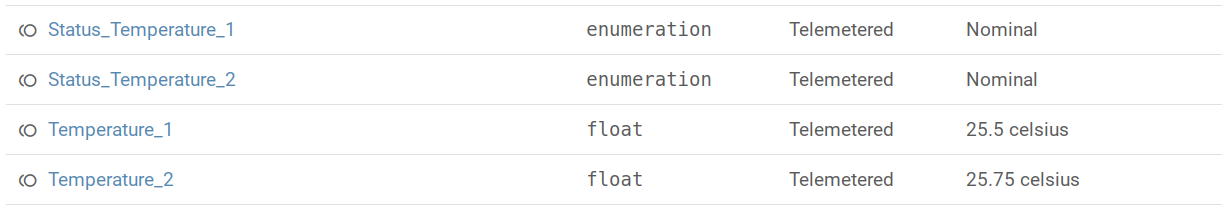
\includegraphics{screenshots/yamcs_parameters}
	\caption{Θερμοκρασιακές παράμετροι \acs{YAMCS} σε κανονική λειτουργία}
	\label{fig:yamcsparametersnominal}
\end{figure}

\begin{figure}[h]
	\centering
	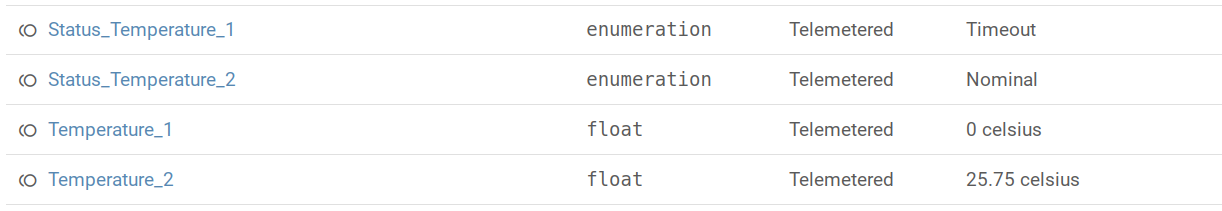
\includegraphics{screenshots/yamcs_f010_parameters}
	\caption{Θερμοκρασιακές παράμετροι \acs{YAMCS} υπό την αποτυχία \texttt{F-010}}
	\label{fig:yamcsparametersf010}
\end{figure}

Στο \Cref{fig:yamcsparametersnominal}, φαίνονται οι τιμές θερμοκρασίας και κατάστασης σε κανονική λειτουργία. Οι τιμές λαμβάνονται κανονικά και οι αισθητήρες αποστέλλουν δεδομένα. Τη στιγμή που αποσυνδέσουμε το καλώδιο, το σύστημα\footnote{\g{Η διαδικασία αυτή πραγματοποιείται από τον οδηγό του περιφερειακού, και όχι από την υλοποίηση των} \acs{ECSS} services.} θέτει την τιμή κατάστασης σε \texttt{TIMEOUT}, καθώς αναγνωρίζει την αποτυχία της ζεύξης (\Cref{fig:yamcsparametersf010}). \g{Ταυτόχρονα, η τιμή της θερμοκρασίας γίνεται \emph{0}, καθώς δεν υπάρχει κάποια ενεργή μέτρηση.\footnote{\g{Σε ένα πραγματικό σύστημα θα είχε νόημα και να διατηρείται η προηγούμενη τιμή της θερμοκρασίας. Σε εμάς η τιμή τέθηκε στο 0 για να επιβεβαιώσουμε πως ένα αποτυχημένο περιφερειακό που επιστρέφει λανθασμένες τιμές δεν μπορεί να επηρεάσει αρνητικά το υπόλοιπο σύστημα.}}}

\begin{figure}[h]
	\centering
	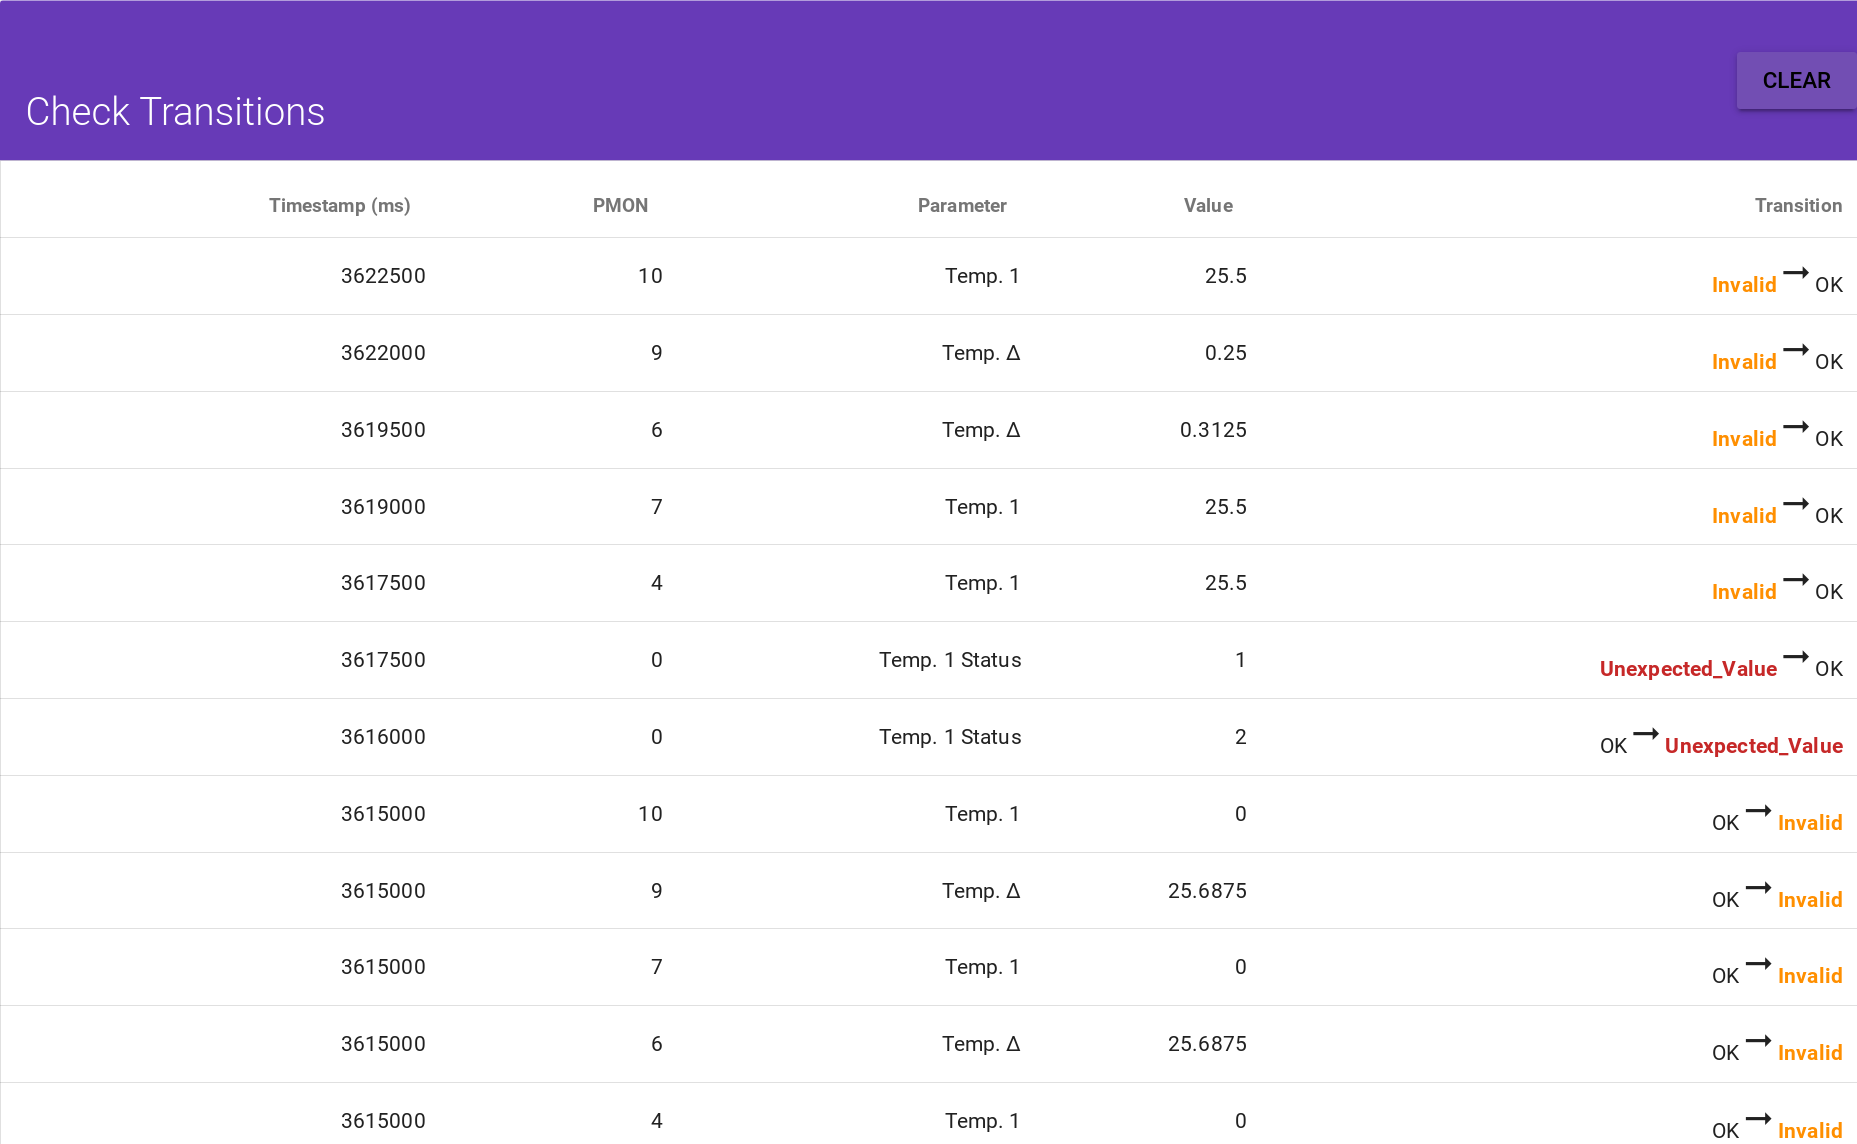
\includegraphics{screenshots/pus_f010_tran}
	\caption{Πίνακας μετάβασης ορισμών παρακολούθησης (αποτυχία \texttt{F-010} όπως φαίνεται στη διεπαφή \acs{PUS})}
	\label{fig:pusf010tran}
\end{figure}

\begin{table*}[h]
	\centering
	\caption[][10pt]{Πίνακας μετάβασης ορισμών παρακολούθησης (αποτυχία \texttt{F-010})}
	\label{tab:f010tran}
	\begin{tabularx}{\linewidth}{@{}S[table-format=4.0]c@{\hskip 3em}rcl@{\hskip 3em}X@{}}
		\toprule
		Χρόνος (ms) & \acs{PMON} & \multicolumn{3}{c}{Παράμετρος} & Μετάβαση \\ \midrule
		0 & 4 & Θερμ. 1 & = & 0 & \ok \ar \invalid \\
		0 & 6 & Θερμ. Δ & = & 25.6875 & \ok \ar \invalid \\
		0 & 7 & Θερμ. 1 & = & 0 & \ok \ar \invalid \\
		0 & 9 & Θερμ. Δ & = & 25.6875 & \ok \ar \invalid \\
		0 & 10 & Θερμ. 1 & = & 0 & \ok \ar \invalid \\
		1000 & 0 & Κατάστ. Θερμ. 1 & = & \texttt{TIMEOUT} & \ok \ar \unexpected \\[1ex]
		\multicolumn{6}{c}{\textcolor{MaterialGrey500}{Αποκατάσταση βλάβης}}\\[1ex]
		2500 & 0 & Κατάστ. Θερμ. 1 & = & \texttt{NOMINAL} & \unexpected \ar \ok \\
		2500 & 4 & Θερμ. 1 & = & 25.5 & \invalid \ar \ok \\
		4000 & 7 & Θερμ. 1 & = & 25.5 & \invalid \ar \ok  \\
		4500 & 6 & Θερμ. Δ & = & 0.3125 & \invalid \ar \ok  \\
		7000 & 9 & Θερμ. Δ & = & 0.25 & \invalid \ar \ok  \\
		7000 & 10 & Θερμ. 1 & = & 25.5 & \invalid \ar \ok  \\ \bottomrule
	\end{tabularx}
\end{table*}

Μετά από την αλλαγή των τιμών των παραμέτρων, σειρά έχει η υπηρεσία \emph{\texttt{ST[12]} on-board monitoring} \g{και οι ορισμοί παρακολούθησης (\Cref{fig:pusf010tran,tab:f010tran}). Εδώ με τη σειρά γίνονται τα εξής:}
\begin{enumerate}
	\item Με το που αποσυνδέεται ο αισθητήρας, οι ορισμοί 4, 6, 7, 9 και 10 (\cref{tab:demo_monitoring}) αποκτούν κατάσταση \invalid. Αυτό συμβαίνει καθώς για αυτούς τους ορισμούς υπάρχει \textbf{συνθήκη εγκυρότητας ελέγχου}. Αν ο αισθητήρας 1 είναι απενεργοποιημένος, \footnote{είτε λόγω προβλήματος, είτε λόγω εντολής} δεν έχει κανένα νόημα η λήψη των τιμών του για εύρεση λαθών.
	
	Επομένως, όλοι οι ορισμοί που συνδέονται με τον αισθητήρα 1 απενεργοποιούνται και δεν μπορούν να πυροδοτήσουν κάποια αντίδραση. Αυτό γίνεται άμεσα.
	\item Μετά από δύο μετρήσεις και χρόνο \( 2 \cdot 500 = \SI{1000}{\milli\second} \), ο ορισμός παρακολούθησης 0 επιβεβαιώνει πως η παράμετρος \emph{Κατάσταση Θερμοκρασία 1} έχει ανεπιθύμητη τιμή. Ως αποτέλεσμα, ο ορισμός παρακολούθησης μεταβαίνει σε κατάσταση \unexpected, και πυροδοτεί όλη τη διαδικασία αναφοράς και διόρθωσης της βλάβης. Η αποτυχία του αισθητήρα έχει πλέον εντοπιστεί, και το σύστημα \acs{FDIR} έχει αρχίσει να δρα.
	\item Οι ορισμοί παρακολούθησης δεν μεταβάλλονται μέχρι να διορθωθεί η βλάβη, οπότε και επιστρέφουν στην κατάσταση \ok όπου δεν υπάρχει κανένα πρόβλημα. Εδώ, όπως θα περιγραφεί αργότερα, το σύστημα αποκατέστησε τη βλάβη χωρίς την επέμβαση του χειριστή, και έχει επιστρέψει στην αρχική του κατάσταση.
\end{enumerate}

\begin{figure}
	\centering
	\caption[Πλήρης λίστα των ορισμών παρακολούθησης κατά την αποτυχία \texttt{F-010}]{Πλήρης λίστα των ορισμών παρακολούθησης κατά την αποτυχία \texttt{F-010}, όπως φαίνονται στην διεπαφή 
	\acs{PUS}. Ο ορισμός \texttt{0} που περιμένει την αποτυχία του αισθητήρα 1 έχει ενεργοποιηθεί, ενώ άλλοι ορισμοί που εξαρτώνται από τον αισθητήρα είναι απενεργοποιημένοι (\invalid).}
	\label{fig:pusf010moni}
	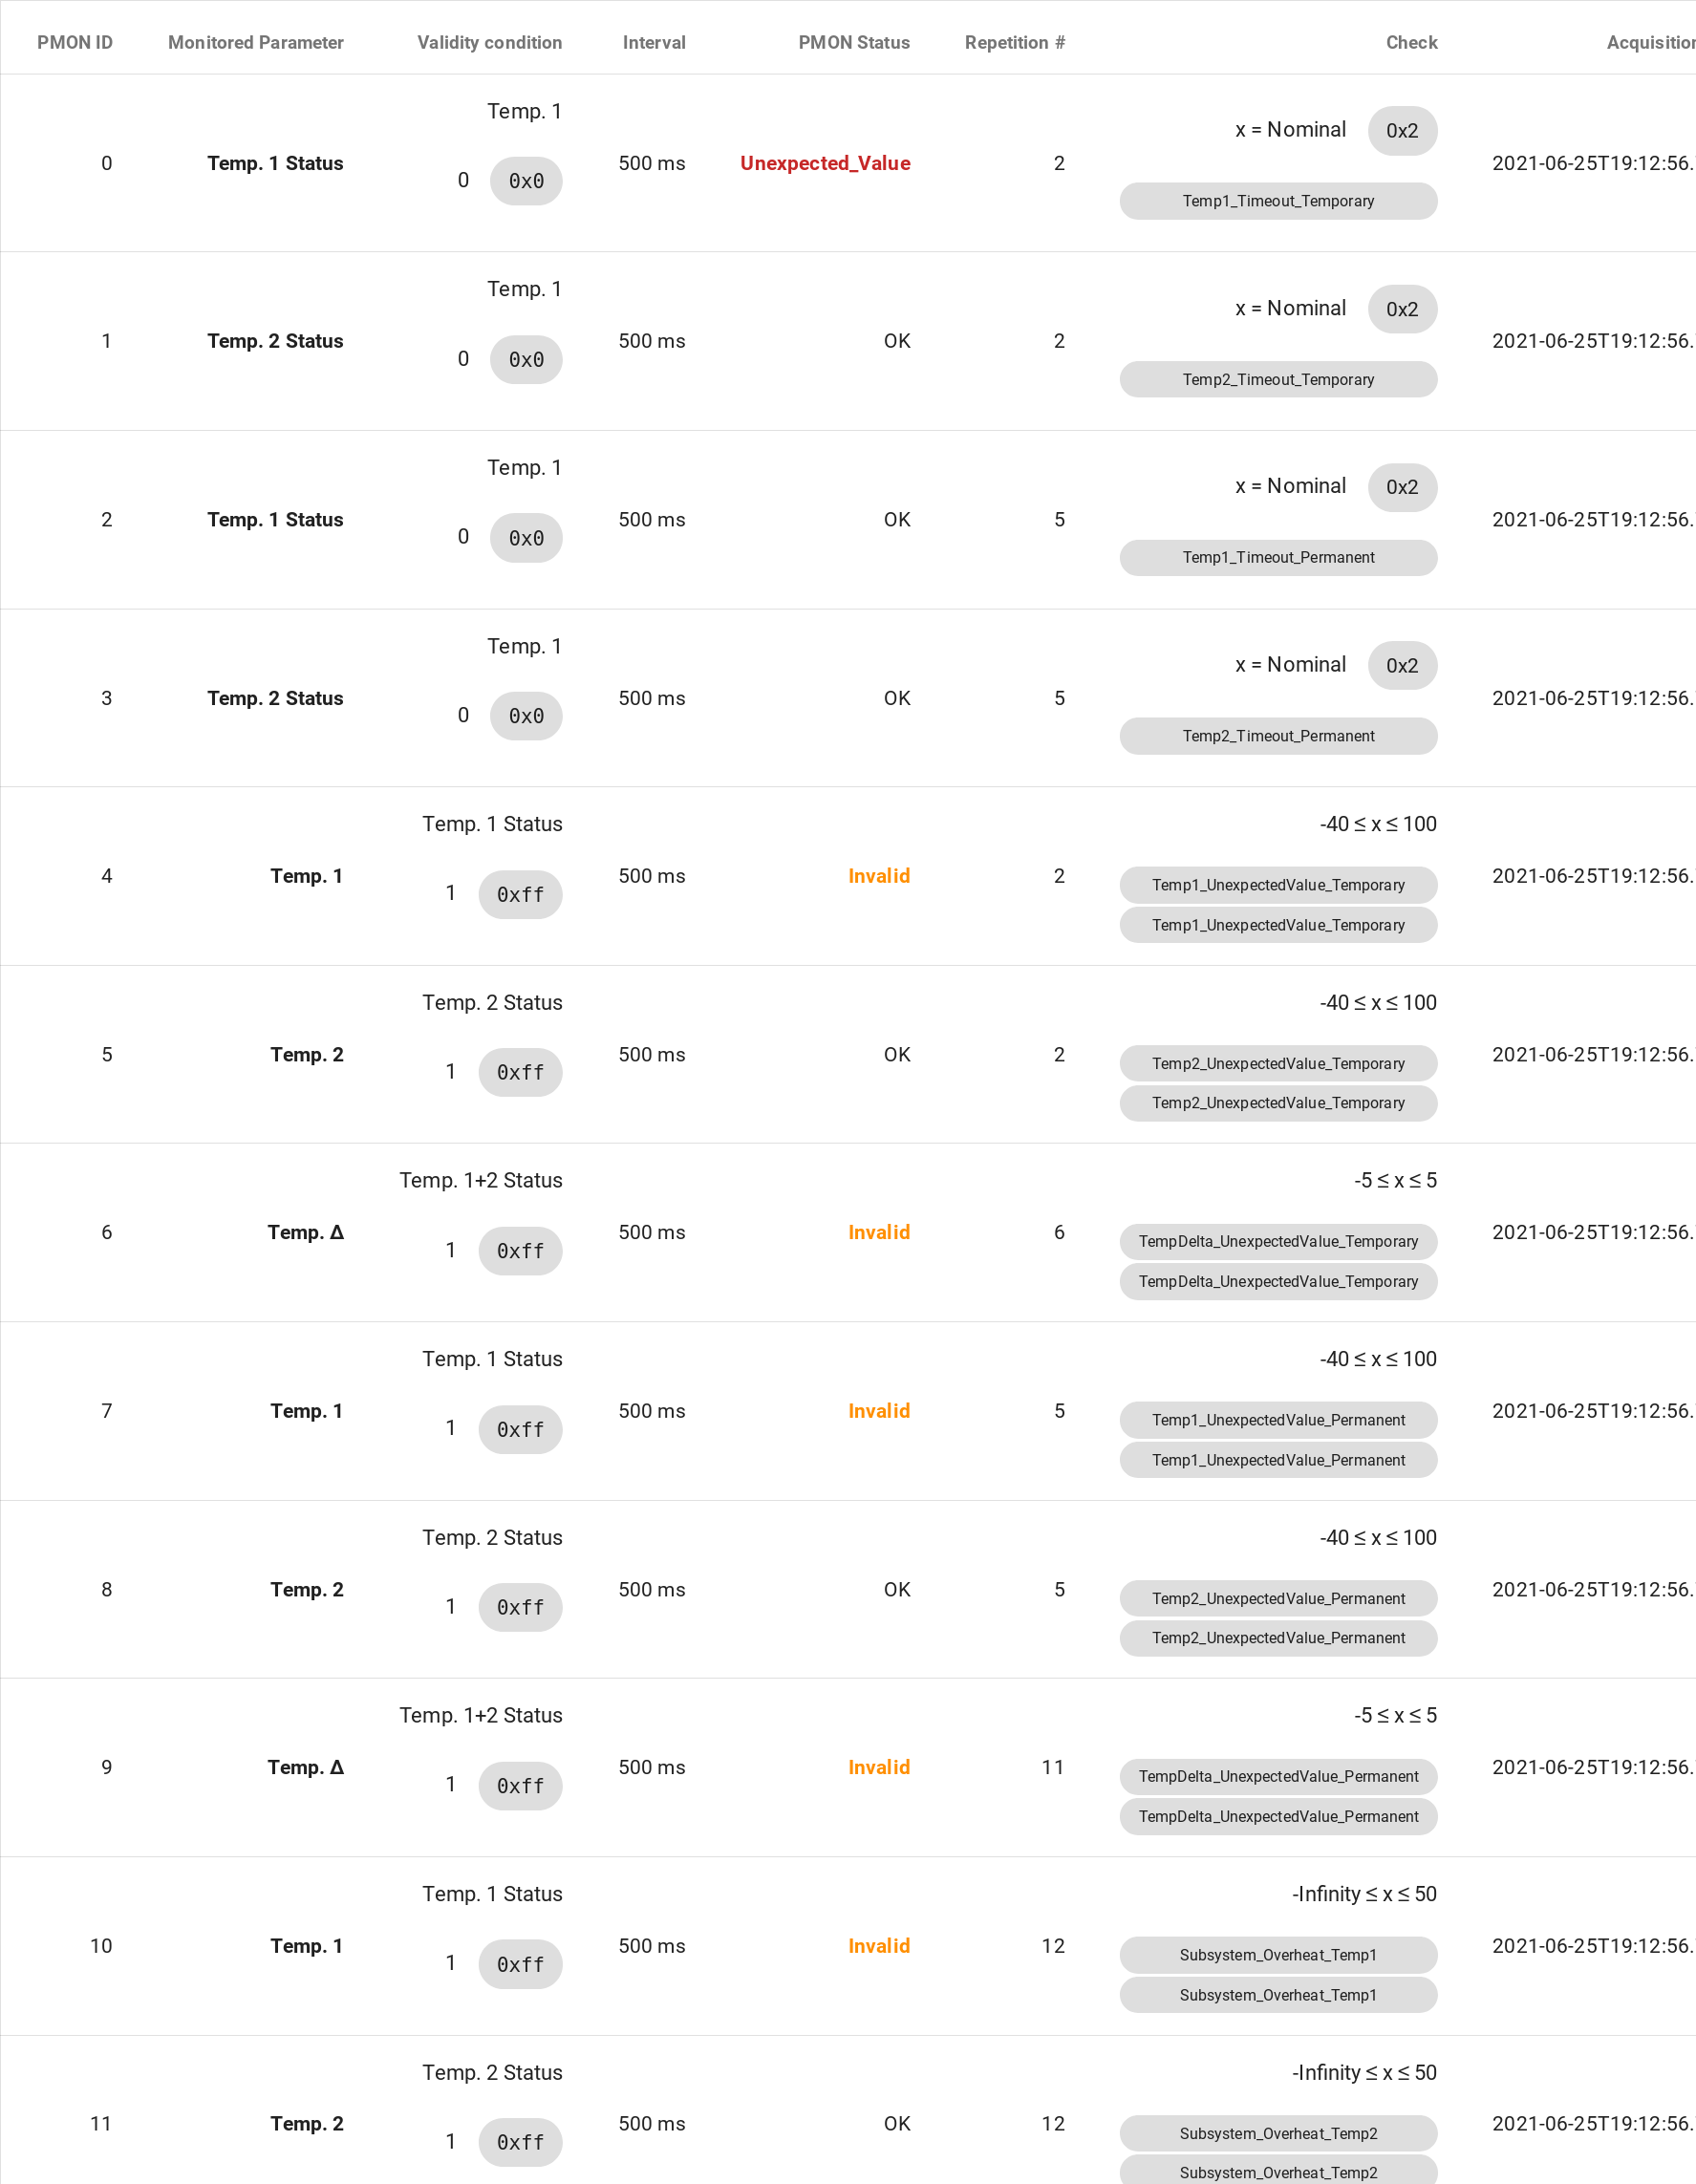
\includegraphics[width=.8\textwidth]{media/screenshots/pus_f010_moni}
\end{figure}

Μετά από τον εντοπισμό της αποτυχίας, δημιουργείται το αντίστοιχο \textbf{γεγονός} και αποστέλλεται στους χειριστές (\Cref{fig:yamcsf010event}).

\begin{figure*}
	\centering
	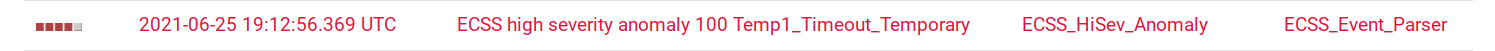
\includegraphics{media/screenshots/yamcs_f010_event}
	\caption[][-10pt]{Το γεγονός προσωρινής αποτυχίας του αισθητήρα όπως φαίνεται στο \acs{YAMCS}}
	\label{fig:yamcsf010event}
\end{figure*}

\g{Με την αποστολή του γεγονότος, πυροδοτείται ο μηχανισμός γεγονότος-αντίδρασης. Η αντίδραση που συνδέεται με την προσωρινή αποτυχία του αισθητήρα είναι η κλήση της συνάρτησης} \texttt{restart\_sensor}\footnote{Υπηρεσία \emph{\texttt{ST[08]} function management}} με όρισμα \texttt{1}, που σηματοδοτεί την επανεκκίνηση του 1\textsuperscript{ου} αισθητήρα. Στους ανθρώπινους παρατηρητές, η ενδεικτική λυχνία \textbf{αναβοσβήνει}, \g{καθώς το σύστημα επανεκκίνησε την τροφοδοσία του αισθητήρα. Αυτή ήταν η πρώτη προσπάθεια για επιδιόρθωση του προβλήματος.}

Σε αυτό το σημείο, στα πλαίσια του πειράματος, ο εκτελεστής του πειράματος επανασυνδέει τον απομακρυσμένο αισθητήρα, προσομοιώνοντας έτσι την "επιδιόρθωση" του προβλήματος. Οι προσπάθειες επικοινωνίας με τον αισθητήρα είναι πετυχημένες, και το σύστημα θεωρεί πως η βλάβη έχει αποκατασταθεί.

\begin{figure}[h]
	\centering
	\includegraphics{screenshots/yamcs_f010_trend}
	\caption[Προβολή της παραμέτρου θερμοκρασίας στη διάρκεια μιας αποτυχίας]{Προβολή της παραμέτρου θερμοκρασίας στη διάρκεια μιας αποτυχίας. Η τιμή είναι φυσιολογική, πέφτει στους \SI{0}{\celsius} για 1 δευτερόλεπτο, και επανέρχεται μετά την επιδιόρθωση.}
	\label{fig:yamcsf010trend}
\end{figure}

\begin{figure}
	\begin{cminted}{text}
3622076 [debug  ] T [T1]: 25.56
3622176 [debug  ] T [T2]: 25.56
3622206 [error  ] Error in TWI: 1
3622206 [debug  ] T [T1]: 0.00
3622307 [debug  ] T [T2]: 25.56
3622336 [error  ] Error in TWI: 1
3622336 [debug  ] T [T1]: 0.00
3622438 [debug  ] T [T2]: 25.63
3622467 [error  ] Error in TWI: 1
3622467 [debug  ] T [T1]: 0.00
3622500 [error  ] Monitoring status 4 changed from 0 to 2
3622500 [error  ] Monitoring status 6 changed from 0 to 2
3622501 [error  ] Monitoring status 7 changed from 0 to 2
3622502 [error  ] Monitoring status 9 changed from 0 to 2
3622502 [error  ] Monitoring status 10 changed from 0 to 2
3622503 [trace  ] New TM [3,25]
Received TM [25]
3622569 [debug  ] T [T2]: 25.63
3622597 [error  ] Error in TWI: 1
3622597 [debug  ] T [T1]: 0.00
3622655 [trace  ] New TM [12,12]
Received TM [82]
3622700 [debug  ] T [T2]: 25.56
3622728 [error  ] Error in TWI: 1
3622728 [debug  ] T [T1]: 0.00
3622831 [debug  ] T [T2]: 25.56
3622859 [error  ] Error in TWI: 1
3622859 [debug  ] T [T1]: 0.00
...
	\end{cminted}
	\caption[Διαγνωστική έξοδος του μικροελεγκτή κατά την αποτυχία \texttt{F-010}]{Διαγνωστική έξοδος του μικροελεγκτή κατά την αποτυχία \texttt{F-010}. Μόλις το καλώδιο αποσυνδεθεί, ο μικροελεγκτής εντοπίζει το σφάλμα στον δίαυλο \acs{I2C}, και η τιμή της αναγνώσιμης θερμοκρασίας γίνεται μηδενική. Η κατάσταση των ορισμών παρακούθησης αλλάζει στον αντίστοιχο χτύπο ρολογιού. Ταυτόχρονα, δημιουργούνται οι τηλεμετρίες ραδιοφάρου (\texttt{[3,25]}) και αναφοράς των μεταβάσεων (\texttt{ST[12,12]}). Τα διαγνωστικά αυτά δεδομένα παράγονται σε μορφή κειμένου από το μικροελεγκτή και δεν θα είναι διαθέσιμα σε τροχιά.}
\end{figure}

\clearpage
\paragraph{\textbf{\texttt{F-020}: Μόνιμη απώλεια λειτουργικότητας}}~

Αυτή η βλάβη είναι παρόμοια με την \texttt{F-010}, αλλά υποθέτει πως το εξάρτημα δεν δύναται να επιδιορθωθεί, ακόμα και μετά την επανεκκίνηση.

\subparagraph{Διαδικασία}
\begin{compactenum}
	\item Αποσυνδέουμε το καλώδιο \acs{SDA} ή \acs{SCL} από το breadboard
\end{compactenum}

\subparagraph{Οπτική ένδειξη} Η 1\textsuperscript{η} ενδεικτική λυχνία αναβοσβήνει μια φορά, παραμένει ανοιχτή, και μετά σβήνει μόνιμα.

\subparagraph{Αποτελέσματα}

\begin{table*}[h]
	\centering
	\caption{Πίνακας μετάβασης ορισμών παρακολούθησης (αποτυχία \texttt{F-020})}
	\label{tab:f020tr}
	\begin{tabularx}{\linewidth}{@{}S[table-format=1.1]c@{\hskip 3em}rcl@{\hskip 3em}X@{}}
		\toprule
		Χρόνος (s) & \acs{PMON} & \multicolumn{3}{c}{Παράμετρος} & Μετάβαση \\ \midrule
		0 & 4 & Θερμ. 1 & = & 0 & \ok \ar \invalid \\
		0 & 6 & Θερμ. Δ & = & 29.9375 & \ok \ar \invalid \\
		0 & 7 & Θερμ. 1 & = & 0 & \ok \ar \invalid \\
		0 & 9 & Θερμ. Δ & = & 29.9375 & \ok \ar \invalid \\
		0 & 10 & Θερμ. 1 & = & 0 & \ok \ar \invalid \\
		1 & 0 & Κατάστ. Θερμ. 1 & = & \texttt{TIMEOUT} & \ok \ar \unexpected \\%[1ex]
		2.5 & 2 & Κατάστ. Θερμ. 1 & = & \texttt{TIMEOUT} & \ok \ar \unexpected \\[1ex]
		\multicolumn{6}{c}{\textcolor{MaterialGrey500}{Απομόνωση βλάβης}}\\[1ex]
		4 & 0 & Κατάστ. Θερμ. 1 & = & \texttt{DISABLED} & \unexpected \ar \ok \\
		5.5 & 2 & Κατάστ. Θερμ. 1 & = & \texttt{DISABLED} & \unexpected \ar \ok \\
		\bottomrule
	\end{tabularx}
	\vspace{10pt}
\end{table*}

Στη δοκιμή αυτή το σύστημα αναγνωρίζει κανονικά την αποτυχία του αισθητήρα, και, όπως φαίνεται στον \Cref{tab:f020tr}, προσπαθεί να την διορθώσει δύο φορές:
\begin{enumerate}
	\item (\( t = \SI{1}{\second} \)) Όπως και στην αποτυχία \texttt{F-010}, \g{γίνεται μία επανεκκίνηση του αισθητήρα. Μετά την επανεκκίνηση, η παράμετρος} \emph{Κατάσταση Θερμοκρασία 1} συνεχίζει να έχει μη αναμενόμενη τιμή, οπότε η διαδικασία του \acs{FDIR} δεν διακόπτεται.
	\item (\( t = \SI{2.5}{\second} \)) Ο ορισμός παρακολούθησης \texttt{2} έχει μετρήση την κατάσταση του αισθητήρα 5 φορές (repetition number), \g{χωρίς καμία επιτυχία. Το σύστημα θεωρεί πως η βλάβη δεν μπορεί να διορθωθεί, και \textbf{απενεργοποιεί} πλήρως την τροφοδοσία του αισθητήρα.}
	
	Με αυτήν τη μέθοδο, η βλάβη απομονώνεται και δεν μπορεί να επηρεάσει το υπόλοιπο σύστημα. Όλοι οι ορισμοί του \acs{FDIR} που συνδέονται με τον αισθητήρα είναι απενεργοποιημένοι. Ο σταθμός βάσης γνωρίζει μέσω τηλεμετρίας την κατάσταση του αισθητήρα, και δεν λαμβάνει υπ' όψιν τις λανθασμένες θερμοκρασιακές μετρήσεις του.
\end{enumerate}

Σε αυτό το σημείο, ο ανενεργός αισθητήρας μπορεί να επαναφερθεί μόνο με κάποια τηλεεντολή, ή με επανεκκίνηση του συστήματος. Μέσα από τη διεπαφή του \acs{YAMCS}, ο χρήστης μπορεί να στείλει την εντολή \mintinline{cpp}{/fdirdemo/Set_Temp1_Status(Temperature_Status: "Nominal")} και ο αισθητήρας να ενεργοποιηθεί ξανά.\footnote{Εσωτερικά, αυτή η εντολή καλεί την υπηρεσία \emph{\texttt{ST[20]} parameter management}, και θέτει την παράμετρο \emph{Κατάσταση Θερμοκρασία 1} σε τιμή \texttt{NOMINAL}} Αν ο αισθητήρας συνεχίσει να είναι αποσυνδεδεμένος, παρατηρούμε πως η διαδικασία \acs{FDIR} επαναλαμβάνεται όπως αναμένεται, και απενεργοποιεί ξανά την τροφοδοσία.

Γενικότερα, παρατηρούμε πως η υπηρεσία του \acs{FDIR} δεν προκαλεί κάποιον υποβιβασμό του υπόλοιπου συστήματος, καθώς εκτελείται ως ξεχωριστή διεργασία του \acs{RTOS}.

\clearpage
\paragraph{\textbf{\texttt{F-040}: Προσωρινή αλλαγή τιμής}}~

Αυτή η βλάβη απαιτεί την αλλαγή της τιμής της θερμοκρασίας για ένα χρονικό διάστημα. Καθώς η θερμοκρασία πρέπει να πέσει κάτω των \SI{-40}{\celsius} ή να ανέβει άνω των \SI{100}{\celsius} για να πυροδοτηθεί ο μηχανισμός \acs{FDIR} (\cref{tab:hsia}), η μόνη πρακτική μέθοδος για προσομοίωση αυτής της αποτυχίας είναι η \textbf{εισαγωγή μιας ψεύτικης τιμής μέσω λογισμικού}.

Ο τρόπος με τον οποίο εισάγουμε αναληθείς τιμές είναι \textbf{ένα από τα δύο μπουτόν} της αναπτυξιακής πλακέτας.\footnote{Εναλλακτικά, μπορούν να χρησιμοποιηθούν δοκιμαστικές τηλεεντολές} Πιο συγκεκριμένα, πατώντας το \emph{button 0}, στην θερμοκρασία 1 προστίθεται η τιμή \SI{80}{\celsius}. Πατώντας το \emph{button 1} \g{γίνεται το αντίστοιχο για τη θερμοκρασία 2.}

\subparagraph{Διαδικασία}
\begin{compactenum}
	\item Κρατάμε πατημένο το \emph{button 0} για  μόνο 2 δευτερόλεπτα.
\end{compactenum}

\subparagraph{Οπτική ένδειξη} Η 1\textsuperscript{η} ενδεικτική λυχνία αναβοσβήνει μία φορά, και παραμένει ανοιχτή.

\subparagraph{Αποτελέσματα}

\begin{table*}[h]
	\centering
	\caption{Πίνακας μετάβασης ορισμών παρακολούθησης (αποτυχία \texttt{F-040})}
	\label{tab:f040tran}
	\begin{tabularx}{\linewidth}{@{}S[table-format=4.0]c@{\hskip 3em}rcl@{\hskip 3em}X@{}}
		\toprule
		Χρόνος (ms) & \acs{PMON} & \multicolumn{3}{c}{Παράμετρος} & Μετάβαση \\ \midrule
		0 & 4 & Θερμ. 1 & = & 109.4375 & \ok \ar \hilim \\[1ex]
		\multicolumn{6}{c}{\textcolor{MaterialGrey500}{Αποκατάσταση βλάβης}}\\[1ex]
		1.5 & 4 & Θερμ. 1 & = & 29.5625 & \hilim \ar \ok \\
		\bottomrule
	\end{tabularx}
	\vspace{10pt}
\end{table*}

Στο παρόν παράδειγμα, μόνο ένας ορισμός \g{παρακολούθησης} βγαίνει εκτός ορίων λόγω της λάθος τιμής. Με το που η έξοδος από τα όρια εντοπιστεί, πραγματοποιείται επανεκκίνηση του αισθητήρα, και η βλάβη αποκαθίσταται.

Η λογική που χρησιμοποιήσαμε στην αρχιτεκτονική του \acs{FDIR} \g{σημαίνει πως οι υπόλοιποι ορισμοί συνεχίζουν να παρακολουθούν την τιμή της θερμοκρασίας του αισθητήρα, χωρίς να λαμβάνουν τιμή} \invalid. Για να αποφευχθεί τυχόν σύγκρουση μεταξύ των ορισμών, θα πρέπει ο αριθμός επαναλήψεων των μετρήσεών τους να είναι μεγαλύτερος από αυτόν που πυροδοτήθηκε τώρα. Πράγματι, στο πείραμα αυτό, δεν μεταβλήθηκε κανένας άλλος ορισμός πριν και μετά τη διόρθωση του σφάλματος.\footnote{Εναλλακτικά, ο έλεγχος εγκυρότητας των υπόλοιπων ορισμών μπορεί να βεβαιώνεται πως η τιμή δεν παραβιάζει τα όρια κάποιου άλλου ορισμού.}

\begin{figure*}[h]
	\centering
	\includegraphics[width=\textwidth]{screenshots/yamcs_f040_trend}
	\caption[Προβολή της παραμέτρου θερμοκρασίας στη διάρκεια της αποτυχίας \texttt{F-040}]{Προβολή της παραμέτρου θερμοκρασίας στη διάρκεια της αποτυχίας \texttt{F-040}. Φαίνεται η υπερβολικά μεγάλη τιμή που εισήγαγε το λογισμικό.}
	\label{fig:yamcsf040trend}
\end{figure*}

\clearpage
\paragraph{\textbf{\texttt{F-050}: Μόνιμη αλλαγή τιμής}}~

Αυτή η βλάβη απαιτεί είναι αντίστοιχη της \texttt{F-040}, χωρίς δυνατότητα επιδιόρθωσης του αισθητήρα.

\subparagraph{Διαδικασία}
\begin{compactenum}
	\item Κρατάμε πατημένο το \emph{button 0} μέχρι να απενεργοποιηθεί η ενδεικτική λυχνία του 1\textsuperscript{ου} αισθητήρα.
\end{compactenum}

\subparagraph{Οπτική ένδειξη} Η 1\textsuperscript{η} ενδεικτική λυχνία αναβοσβήνει μια φορά, παραμένει ανοιχτή, και μετά σβήνει μόνιμα.

\subparagraph{Αποτελέσματα}

\begin{table*}[h]
	\centering
	\caption[]{Πίνακας μετάβασης ορισμών παρακολούθησης (αποτυχία \texttt{F-050})}
	\label{tab:f050tran}
	\begin{tabularx}{\linewidth}{@{}S[table-format=4.0]c@{\hskip 3em}rcl@{\hskip 3em}X@{}}
		\toprule
		Χρόνος (ms) & \acs{PMON} & \multicolumn{3}{c}{Παράμετρος} & Μετάβαση \\ \midrule
		0 & 4 & Θερμ. 1 & = & 109.4375 & \ok \ar \hilim \\
		1.5 & 7 & Θερμ. 1 & = & 109.4375 & \ok \ar \hilim \\[1ex]
		\multicolumn{6}{c}{\textcolor{MaterialGrey500}{Απομόνωση βλάβης}}\\[1ex]
		1.5 & 9 & Θερμ. Δ & = & -79.9375 & \ok \ar \invalid \\
		1.5 & 10 & Θερμ. 1 & = & 109.4375 & \ok \ar \invalid \\
		2 & 4 & Θερμ. 1 & = & 109.4375 & \hilim \ar \invalid \\
		2 & 6 & Θερμ. Δ & = & -79.9375 & \ok \ar \invalid \\
		2 & 7 & Θερμ. 1 & = & 109.4375 & \hilim \ar \invalid \\
		\bottomrule
	\end{tabularx}
	\vspace{10pt}
\end{table*}

Η διαδικασία \acs{FDIR} εδώ ακολουθεί ξανά δύο στάδια:
\begin{enumerate}
	\item Μετά τον πρώτο εντοπισμό (ορισμός \texttt{4}), γίνεται επανεκκίνηση του αισθητήρα, και η ενδεικτική λυχνία αναβοσβήνει. Παρ' όλα αυτά, το πρόβλημα δεν αποκαθίσταται.
	\item Μετά από \SI{1.5}{\second} επιπλέον δευτερόλεπτα, αναλαμβάνει δράση ο ορισμός \texttt{7}. Αφού ο αισθητήρας έχει ακόμα μία αφύσικη τιμή θερμοκρασίας, η αντίδραση είναι ο αισθητήρας να απενεργοποιηθεί. Έχει ξεκινήσει έτσι η απομόνωση της αποτυχίας.
	
	Μετά από την απομόνωση, όπου η κατάσταση του περιφερειακού τίθεται σε \texttt{DISABLED}, οι ορισμοί που εξαρτώνται από αυτό το περιφερειακό απενεργοποιούνται (\invalid). Όπως είναι αναμενόμενο, η απομόνωση έχει ολοκληρωθεί.
\end{enumerate}

Τα βήματα διόρθωσης και απομόνωσης είναι αντίστοιχα με αυτά της αποτυχίας \texttt{F-020}, και απαιτείται ξανά επέμβαση από τους χειριστές για οποιαδήποτε άλλη κίνηση.

\clearpage
\paragraph{\textbf{\texttt{F-040} και \texttt{F-050}: Διαφορική μέτρηση}}~

Οι αποτυχίες \texttt{F-040} και \texttt{F-050} έχουν έναν δεύτερο τρόπο εντοπισμού: Τη \emph{μεγάλη διαφορά μεταξύ μετρήσεων των 2 αισθητήρων}. Δεδομένου του μικρού κατωφλίου που ορίζεται στον \Cref{tab:hsia} (\(|Δ| \leq \SI{5}{\celsius} \)), η δοκιμή αυτή γίνεται στο υλικό, θερμαίνοντας έναν από τους 2 αισθητήρες.

\subparagraph{Διαδικασία}
\begin{compactenum}
	\item Θερμαίνουμε έναν αισθητήρα με κάποιο θερμαντικό σώμα. Φροντίζουμε ώστε να μην θερμανθεί πολύ (\(<\SI{50}{\celsius}\)), και η θερμότητα να είναι εστιασμένη μόνο σε αυτόν.
\end{compactenum}

\subparagraph{Οπτική ένδειξη (προσωρινή αποτυχία)} \g{Και οι δύο ενδεικτικές λυχνίες αναβοσβήνουν ταυτόχρονα μια φορά, και παραμένουν ανοιχτές.}

\subparagraph{Οπτική ένδειξη (μόνιμη αποτυχία)} Και οι δύο ενδεικτικές λυχνίες αναβοσβήνουν ταυτόχρονα μια φορά, παραμένουν ανοιχτές, και μετά σβήνουν μόνιμα.

\subparagraph{Αποτελέσματα}
\begin{table*}[h]
	\centering
	\caption{Πίνακας μετάβασης ορισμών παρακολούθησης (προσωρινή αποτυχία \texttt{F-040}, διαφορική)}
	\label{tab:f040dtran}
	\begin{tabularx}{\linewidth}{@{}S[table-format=4.0]c@{\hskip 3em}rcl@{\hskip 3em}X@{}}
		\toprule
		Χρόνος (ms) & \acs{PMON} & \multicolumn{3}{c}{Παράμετρος} & Μετάβαση \\ \midrule
		0 & 6 & Θερμ. Δ & = & -6.1875 & \ok \ar \lolim \\[1ex]
		\multicolumn{6}{c}{\textcolor{MaterialGrey500}{Αποκατάσταση βλάβης}}\\[1ex]
		7.5 & 6 & Θερμ. Δ & = & -4.8125 & \lolim \ar \ok \\
		\bottomrule
	\end{tabularx}
	\vspace{10pt}
\end{table*}

Οι ενέργειες διόρθωσης που σημειώνονται στην διαφορική περίπτωση είναι παρόμοιες με αυτές τις απλής περίπτωσης (\texttt{F-040}, \texttt{F-050}), με τη διαφορά πως δεν είναι γνωστό ποιός από τους 2 αισθητήρες έχει αποτύχει. Η προσέγγιση που ακολουθεί η αρχιτεκτονική εδώ είναι \emph{fail-safe}, και απενεργοποιεί και τους 2 αισθητήρες. Ως συνέπεια, οι 7 ορισμοί παρακολούθησης που εξαρτώνται από θερμοκρασιακές τιμές απενεργοποιούνται (\invalid).

\begin{table*}[h]
	\centering
	\caption{Πίνακας μετάβασης ορισμών παρακολούθησης (μόνιμη αποτυχία \texttt{F-050}, διαφορική) \draft{repeat measurements}}
	\label{tab:f050dtran}
	\begin{tabularx}{\linewidth}{@{}S[table-format=4.0]c@{\hskip 3em}rcl@{\hskip 3em}X@{}}
		\toprule
		Χρόνος (ms) & \acs{PMON} & \multicolumn{3}{c}{Παράμετρος} & Μετάβαση \\ \midrule
		0 & 6 & Θερμ. Δ & = & -5.8125 & \ok \ar \lolim \\
		?? & 6 & Θερμ. Δ & = & -6.6875 & \ok \ar \lolim \\[1ex]
		\multicolumn{6}{c}{\textcolor{MaterialGrey500}{Απομόνωση βλάβης}}\\[1ex]
		??? & ? & Θερμ. Δ & = & -4.8125 & \ok \ar \invalid \\
		??? & ? & Θερμ. Δ & = & -4.8125 & \ok \ar \invalid \\
		??? & ? & Θερμ. Δ & = & -4.8125 & \ok \ar \invalid \\
		??? & ? & Θερμ. Δ & = & -4.8125 & \ok \ar \invalid \\
		??? & ? & Θερμ. Δ & = & -4.8125 & \ok \ar \invalid \\
		??? & ? & Θερμ. Δ & = & -4.8125 & \ok \ar \invalid \\
		??? & ? & Θερμ. Δ & = & -4.8125 & \ok \ar \invalid \\
		\bottomrule
	\end{tabularx}
	\vspace{10pt}
\end{table*}

\FloatBarrier
\paragraph{\textbf{\texttt{F-060}: Κολλημένος ακροδέκτης εξόδου \acs{I2C}}}~
Αυτή η αποτυχία προσομοιώνεται με σύνδεση υλικού. Σε τέτοιες περιπτώσεις πρέπει να δίνεται προσοχή ώστε να μη γίνονται συνδέσεις (π.χ. βραχυκυκλώματα) που θα βλάψουν το δοκιμαστικό σύστημα, ειδικά αν δεν υπάρχουν κατάλληλα κυκλώματα προστασίας.

\subparagraph{Διαδικασία}
\begin{compactenum}
	\item Συνδέουμε έναν από τους ακροδέκτες \acs{SDA}, \acs{SCL} στη γείωση με ένα επιπλέον καλώδιο.\footnote{Καθώς το \acs{I2C} λειτουργεί με βάση τη λογική ανοιχτής εκροής (open drain), η σύνδεση στη γείωση δεν θα προκαλέσει πρόβλημα στα ηλεκτρονικά.}
\end{compactenum}

\subparagraph{Αποτελέσματα}
Παρατηρούμε πως τα αποτελέσματα είναι ακριβώς ίδια με αυτά τις αποτυχίας \texttt{F-020} (μόνιμη απώλεια λειτουργικότητας). Αυτό είναι φυσιολογικό, καθώς ουσιαστικά καταστρέφουμε τον δίαυλο \acs{I2C} του περιφερειακού.

\paragraph{\textbf{\texttt{F-070} μέχρι \texttt{F-120}: Αισθητήρας 2}}~

Τα αποτελέσματα των δοκιμών \acs{FDIR} για τον 2\textsuperscript{ο} αισθητήρα είναι ίδια με αυτά του 1\textsuperscript{ου} αισθητήρα που παρουσιάστηκαν παραπάνω, καθώς τα εξαρτήματα έχουν ίδια συμπεριφορά και σχεδιασμό \acs{FDIR}.

Σε αυτό το σημείο σημειώνεται πως ακόμα κι αν ο σχεδιασμός και το λογισμικό είναι πανομοιότυπα, σε περιπτώσεις σαν και αυτήν υπάρχει νόημα επανάληψης των δοκιμών για τα επιπλέον εξαρτήματα, καθώς συνεχίζει να υπάρχει η πιθανότητα προβλημάτων υλικού, λάθος συνδέσεων, ατυχών ρυθμίσεων και bugs.

\clearpage
\paragraph{\textbf{\texttt{F-130}: Υπερθέρμανση υποσυστήματος}}~
Στη δοκιμή αυτή δεν μελετάμε την αποτυχία ενός από τους αισθητήρες, αλλά την αποτυχία του ίδιου του υποσυστήματος, που υποθέτουμε πως έχει υπερθερμανθεί. Η χαμηλή θερμοκρασία-στόχος (\SI{50}{\celsius}, \cref{tab:hsia}) επιτρέπει την επιβεβαίωση σε υλικό.

\subparagraph{Διαδικασία}
\begin{compactenum}
	\item \g{Χρησιμοποιούμε ένα πιστόλι θερμού αέρα ή κάποια άλλη πηγή θερμότητας ώστε να θερμάνουμε και τους δύο αισθητήρες στους} \SI{50}{\celsius}. \g{Φροντίζουμε ώστε η αύξηση της θερμοκρασίας να είναι ομοιόμορφη, για να μην ενεργοποιηθεί ο έλεγχος διαφοράς.}
\end{compactenum}

\subparagraph{Οπτική ένδειξη} Το LED κατάστασης του μικροελεγκτή σταματά να αναβοσβήνει για λίγο, και έπειτα επανέρχεται.

\subparagraph{Αποτελέσματα}

\begin{table*}[h]
	\centering
	\caption{\draft{todo: repeat measurement}}
	\label{tab:f130tran}
	\begin{tabularx}{\linewidth}{@{}S[table-format=4.0]c@{\hskip 3em}rcl@{\hskip 3em}X@{}}
		\toprule
		Χρόνος (ms) & \acs{PMON} & \multicolumn{3}{c}{Παράμετρος} & Μετάβαση \\ \midrule
		0 & 6 & Θερμ. Δ & = & -5.8125 & \ok \ar \lolim \\
		?? & 6 & Θερμ. Δ & = & -6.6875 & \ok \ar \lolim \\
		\multicolumn{6}{l}{\cellcolor{MaterialYellow300}\textcolor{black}{\acs{MCU} reset}}\\
		\bottomrule
	\end{tabularx}
	\vspace{10pt}
\end{table*}

Εδώ ενεργοποιείται ο ορισμός παρακολούθησης που συνδέεται με τον αισθητήρα που έφτασε στους \SI{50}{\celsius}. Μόλις το σύστημα περάσει αρκετή ώρα σε αυτήν τη θερμοκρασία, γίνεται άμεσα μία επανεκκίνηση του μικροελεγκτή. Η επανεκκίνηση αυτή θα συνεχίσει να γίνεται, μέχρι η θερμοκρασία να επανέλθει.

Η αποτυχία αυτή ουσιαστικά ανήκει στο επίπεδο υποσυστήματος και όχι υλικού που μελετούσαμε προηγουμένως. Σημειώνουμε επίσης πως, λόγω του μεγάλου χρονικού διαστήματος μεταξύ των επανεκκινήσεων, οι χειριστές έχουν αρκετό χρόνο στη διάθεσή τους ώστε να απενεργοποιήσουν το \acs{FDIR} ή να λάβουν και να επεξεργαστούν την τηλεμετρία.

\clearpage
\subsection{Τροποποίηση του \acs{FDIR} σε πραγματικό χρόνο}

Η δύναμη της προσέγγισης \ac{FDIR} του \acs{SAVOIR} έγκειται στο ότι ολόκληρη η δομή \ac{FDIR} μπορεί να τροποποιηθεί με ασφάλεια μέσω τηλεεντολών, χωρίς να απαιτούνται τροποποιήσεις ή επαναφορτώσεις του κώδικα και του λογισμικού. Η εφαρµογή του μοντέλου υπηρεσιών \acs{ECSS} επιτρέπει την προσαρµογή όλων των υπηρεσιών και λειτουργιών \ac{FDIR}, χρησιµοποιώντας προκαθορισµένες δοµές τηλεεντολών. Σε αυτή την ενότητα, θα εκτελεστούν εντολές \acs{ECSS} για την επίδειξη αυτών των δυνατοτήτων και του ελέγχου τους από τον σταθμό βάσης.

\g{Γενικότερα, το επίπεδο της δυνατότητας αναδιαμόρφωσης που παρέχει το σύστημα καθορίζεται από τις απαιτήσεις που παρατίθενται στα \cite{ECSS-E-ST-70-11C,SAVOIR-HB-003}. Η προσαρμοσμένη έκδοση που χρησιμοποιήθηκε για τα πειράματά μας παρατίθεται στον \Cref{tab:fdir-recon-rq}.}

\begin{table*}[h]
	\centering
	\caption[]{Απαιτήσεις αναδιαμόρφωσης \acs{FDIR} στην πειραματική διάταξη}
	\label{tab:fdir-recon-rq}
	\begin{tabularx}{\textwidth}{@{}lXlL{4cm}@{}}
		\toprule
		\# & Προδιαγραφή & Υπηρεσία & Λεπτομέρειες \\ \midrule
		\texttt{RC-010} & Οι αναφορές FDIR πρέπει να περιέχουν όλες τις πληροφορίες για την ανάλυση αποτυχιών (π.χ. ώρα εμφάνισης, παράμετροι εκτός ορίων, πραγματοποιημένες μεταγωγές). & ST[12] on-board monitoring & Μέσω περιοδικών \emph{αναφορών μεταγωγής} \\
		\texttt{RC-020} & Πρέπει να παρέχεται η δυνατότητα ενεργοποίησης και απενεργοποίησης οποιασδήποτε λειτουργίας FDIR μέσω τηλεεντολών. & ST[12] on-board monitoring & Με εντολές \emph{enable}/\emph{disable} \emph{parameter monitoring definitions} \\
		\texttt{RC-030} & Πρέπει να παρέχεται η δυνατότητα προσθήκης και διαγραφής παραμέτρων από τον κατάλογο παρακολούθησης. & ST[12] on-board monitoring & Με εντολές \emph{add}/\emph{delete} \emph{parameter monitoring definitions} \\
		\texttt{RC-040} & Πρέπει να παρέχεται η δυνατότητα τροποποίησης των ενεργειών αποκατάστασης βλάβης που συνδέονται με κάθε ορισμό παρακολούθησης. & ST[19] event-action & Με εντολές \emph{add}, \emph{delete}, \emph{enable} και \emph{disable} \emph{event-action definitions} \\ \bottomrule
	\end{tabularx}
	\vspace{5pt}
\end{table*}

Η πλατφόρμα \ac{YAMCS} χρησιμοποιήθηκε ξανά για τη δημιουργία των επιθυμητών εντολών (\Cref{fig:yamcs_commands}). Παρακάτω, θα αναλυθεί ο τρόπος με τον οποίο μπορεί να επιτευχθεί η κάθε μία από τις παραπάνω απαιτήσεις

\begin{figure}[h]
	\includegraphics{screenshots/yamcs_commands.png}
	\caption[Λίστα τηλεεντολών στο περιβάλλον του \acs{YAMCS}]{Λίστα τηλεεντολών στο περιβάλλον του \acs{YAMCS}. Αυτές οι εντολές μπορούν να εκκινήσουν διαδικασίες στον δορυφόρο, να ενεργοποιήσουν/απενεργοποιήσουν αισθητήρες, ή να αλλάξουν τις ρυθμίσεις των εξαρτημάτων του δορυφόρου. Η λίστα αυτών των εντολών παρέχεται στο \acs{YAMCS} μέσω των αρχείων \ac{XTCE} (\Cref{app:xtce}).}
	\label{fig:yamcs_commands}
\end{figure}

\paragraph{\textbf{\texttt{RC-010} Παρατηρησιμότητα \acs{FDIR}}}~

Ο βαθμός παρατηρησιμότητας που απαιτείται, σε πραγματικό και μη χρόνο, εξασφαλίζεται μέσω της διεπαφής που παρουσιάστηκε στην \Cref{sec:pusinterface}. Οι έτοιμες δομές τηλεμετρίας που υλοποιούνται από το πρότυπο \acs{PUS} \autocite{ECSS-E-ST-70-41C} είναι:
\begin{compactitem}
	\item \texttt{TM[3,25]}: Περιοδική αναφορά τιμών παραμέτρων (ραδιοφάρος)
	\item \texttt{TM[5,1]} μέχρι \texttt{TM[5,4]}: Αναφορά γεγονότων όταν συμβαίνουν
	\item \texttt{TM[12,9]}: Λίστα των ορισμών παρακολούθησης
	\item \texttt{TM[12,12]}: Περιοδική αναφορά μεταβάσεων κατάστασης σε ορισμούς παρακολούθησης\footnote{Πιο απλά, ενημερωνόμαστε πότε μια παράμετρος βγαίνει εκτός ορίων, και πότε επανέρχεται σε κανονική κατάσταση}
	\item \texttt{TM[19,7]} και \texttt{TM[19,11]}: \g{Λίστα των ορισμών γεγονότος-αντίδρασης}
	\item \texttt{TM[20,2]}: Αναφορά της τιμής οποιασδήποτε παραμέτρου του συστήματος
\end{compactitem}

\g{Με το παραπάνω σύνολο τηλεμετρίας, που κατεβαίνει είτε αυτόνομα είτε μετά από εντολή, οι χειριστές έχουν τη δυνατότητα να μελετήσουν την κατάσταση του συστήματος και του} \acs{FDIR} με λεπτομέρεια. Όλα τα αποτελέσματα στην \Cref{sec:simul} εξάχθηκαν χρησιμοποιώντας τις παραπάνω δομές τηλεμετρίας.

\paragraph{\textbf{\texttt{RC-020} Ενεργοποίηση/απενεργοποίηση \acs{FDIR}}}~

Οι δυνατότες που υλοποιήθηκαν και δοκιμάστηκαν για τον έλεγχο του \acs{FDIR} είναι οι εξής:
\begin{itemize}
	\item \texttt{TC[12,16]}: \emph{disable the parameter monitoring function}
	
	Αυτή η τηλεεντολή ορίζεται στο πρότυπο \acs{PUS} και επιτρέπει την πλήρη απενεργοποίηση της παρακολούθησης παραμέτρων, άρα, κατ' επέκτασιν, την \textbf{πλήρη απενεργοποίηση του \acs{FDIR}}. Μετά την αποστολή της, οποιαδήποτε αποτυχία στο σύστημα δεν γίνεται αντιληπτή, και δεν εκτελείται καμία πράξη ανάκαμψης.
	
	Γίνεται αντιληπτό πως μια τέτοια εντολή είναι αρκετά επικίνδυνη για το σύστημα του δορυφόρου, καθώς μία λάθος εκτέλεσή της θα μειώσει κατά πολύ τη δυνατότητα ανάκαμψης από μία βλάβη.\footnote{Για αυτό προτείνεται σε κρίσιμες διαδικασίες να απαιτείται να στέλνονται δύο εντολές σε σειρά (λογική ARM-EXECUTE)} Παρ' όλα αυτά, είναι χρήσιμη σε περίπτωση που το \acs{FDIR} εμφανίζει προβλήματα.
	
	Εδώ σημειώνουμε πως αυτή η εντολή δεν αποτρέπει τα ερωτήματα κατάστασης και τις επιπλέον ρυθμίσεις στην υπηρεσία παρακολούθησης.
	
	\item \texttt{TC[12,15]}: \emph{enable the parameter monitoring function}
	
	\g{Η τηλεεντολή αυτή επιτρέπει την επαναλειτουργία της παρακολούθησης παραμέτρων, αν απενεργοποιήθηκε προηγουμένως.}
	
	\item \texttt{TC[12,1]}: \emph{enable parameter monitoring definitions}
	
	Πέρα από απενεργοποίηση ολόκληρης της λειτουργίας \acs{FDIR}, το πρότυπο δίνει τη δυνατότητα απενεργοποίησης (μαζικής ή μη) μόνο συγκεκριμένων κομματιών του.
	
	\begin{figure}[h]
		\includegraphics{screenshots/yamcs_send_disablepmon.png}
		\caption[Προβολή της οθόνης εκτέλεσης εντολής του \acs{YAMCS}]{Προβολή της οθόνης εκτέλεσης εντολής του \acs{YAMCS}. Ο χρήστης καλείται να εισάγει το ένα όρισμα της εντολής \texttt{TC[12,1]}, που είναι ο ορισμός παρακολούθησης που επιθυμεί να απενεργοποιήσει.}
		\label{fig:yamcssenddisablepmon}
	\end{figure}

	Αυτή η δυνατότητα είναι ιδιαίτερα χρήσιμη, ειδικότερα όταν φαίνεται ότι το \acs{FDIR} είναι υπερβολικά αυστηρό για κάποιο εξάρτημα

	\item \texttt{TC[12,2]}: \emph{disable parameter monitoring definitions}
	
	\item \texttt{TC[19,5]}: \emph{disable event-action definitions}
	
	Πέρα από την απενεργοποίηση ολόκληρου του \acs{FDIR} για ένα εξάρτημα, δίνεται η δυνατότητα απενεργοποίησης μόνο του "IR" κομματιού του. Αυτό σημαίνει πως ενώ γίνεται εντοπισμός των αποτυχιών, δεν γίνεται \textbf{καμία προσπάθεια για απομόνωση ή επιδιόρθωσή τους}. \g{Με αυτόν τον τρόπο μπορούμε να απενεργοποιήσουμε το \acs{FDIR}, αλλά να διατηρήσουμε την παρατηρησιμότητα των παραμέτρων και των ορίων.}
	
	Πιο τεχνικά, η εντολή αυτή απενεργοποιεί τους ορισμούς γεγονότος-αντίδρασης για συγκεκριμένα γεγονότα. Η συμπεριφορά μιας τυπικής αποτυχίας αφού έχει εκτελεστεί αυτή η εντολή φαίνεται στον \Cref{tab:eaofftr}.
	
	\begin{table*}[h]
		\centering
		\caption{Πίνακας μετάβασης με απενεργοποιημένη την υπηρεσία event-action}
		\label{tab:eaofftr}
		\begin{tabularx}{\linewidth}{@{}S[table-format=4.0]c@{\hskip 3em}rcl@{\hskip 3em}X@{}}
			\toprule
			Χρόνος (ms) & \acs{PMON} & \multicolumn{3}{c}{Παράμετρος} & Μετάβαση \\ \midrule
			0 & 4 & Θερμ. 1 & = & 110.625 & \ok \ar \hilim \\
			1.5 & 7 & Θερμ. 1 & = & 110.6875 & \ok \ar \hilim \\
			2 & 6 & Θερμ. Δ & = & -79.9375 & \ok \ar \lolim \\
			4.5 & 9 & Θερμ. Δ & = & -79.875 & \ok \ar \lolim \\
			5 & 10 & Θερμ. Δ & = & 110.625 & \ok \ar \hilim \\
			\bottomrule
		\end{tabularx}
		\vspace{10pt}
	\end{table*}
	
	\item \texttt{TC[19,4]}: \emph{enable event-action definitions}	
	
\end{itemize}

\paragraph{\textbf{\texttt{RC-030} Προσθήκη/διαγραφή ορισμών παρακολούθησης}}~

\draft{todo...}

\paragraph{\textbf{\texttt{RC-040} Προσθήκη/διαγραφή αντιδράσεων}}~

\draft{todo...}

\chapter{Συμπεράσματα και Μελλοντική Εργασία}

\draft{todo...}

\label{cap:conclusion}

% Suggestions for standard:
% hard to play with parameters
% two validity conditions: safe mode etc. how to manage?
% derived parameters (e.g. Δ between sensors)
% event-action definition ID

\section{Μελλοντική εργασία}

\draft{todo...}

%\backmatter
\appendix

\begin{fullwidth}
\bgroup
\printbibliography[heading=bibnumbered,title={Βιβλιογραφία}]
\egroup
\end{fullwidth}


%\printindex

\chapter{Πηγαίος κώδικας}
\label{sec:source_code}

\setminted{
	bgcolor={},
	fontsize=\fontsize{9pt}{9pt},
	linenos
}

%\begin{fullwidth}

\section*{\texttt{analysis.jl}}
\label{app:analysisjl}

\begin{fullwidth}
	\draft{1 γραμμή - επεξήγηση του κάθε αρχείου}
\end{fullwidth}

\inputminted{julia}{analysis/comparisons_el.jl}

\section*{\texttt{main.cpp}}

\inputminted{cpp}{code/main.cpp}

\newpage
\section*{\texttt{SystemParameters.hpp}}

\inputminted{cpp}{code/SystemParameters.hpp}

\newpage
\section*{\texttt{TemperatureTask.cpp}}

\inputminted{cpp}{code/TemperatureTask.cpp}

\section*{\texttt{xtce.xml}}
\label{app:xtce}

\inputminted{xml}{code/xtce-small.xml}

\newpage
\section*{\texttt{ecss-interface.js}}

\inputminted{javascript}{code/ecss-interface.js}

\newpage
\section*{\texttt{link.cpp}}

\inputminted{cpp}{code/link.cpp}

\draft{more files}

\end{document}

